\documentclass[journal]{IEEEtran}

\usepackage{amsmath, amsfonts, amssymb, amscd}
\usepackage[usenames,dvipsnames]{color} 

\usepackage[capitalize]{cleveref}
\usepackage{longtable}
\usepackage{multicol}
\usepackage{pdfpages}
\usepackage[utf8]{inputenc}

\usepackage{graphics}
\usepackage{subfigure}
\usepackage{tikz}

\usepackage{pgfplots}
\usetikzlibrary{pgfplots.fillbetween}
\pgfplotsset{scaled x ticks=false}
\pgfplotsset{compat=newest}
\pgfplotsset{every axis/.append style={axis on top}}
\setlength{\unitlength}{1in} 
\usepgfplotslibrary{groupplots}

\usepackage{nomencl}
\usepackage{enumerate}
\usepackage{cancel}

\usepackage[none]{hyphenat}

\usepackage[style=ieee, url=false, doi=false]{biblatex}
\renewcommand*{\bibfont}{\footnotesize}
\addbibresource{IEEEfull.bib}

%%%%%%%%%%%%%%%%%%%%%%%%%%%%%%
\newif\ifdraft

% For final version, replace next line by \draftfalse
% \drafttrue for draft version with comments
\drafttrue
% \draftfalse
%%%%%%%%%%%%%%%%%%%%%%%%%%%%%

% *** MISC UTILITY PACKAGES ***
%
%\usepackage{ifpdf}
% Heiko Oberdiek's ifpdf.sty is very useful if you need conditional
% compilation based on whether the output is pdf or dvi.
% usage:
% \ifpdf
%   % pdf code
% \else
%   % dvi code
% \fi
% The latest version of ifpdf.sty can be obtained from:
% http://www.ctan.org/pkg/ifpdf
% Also, note that IEEEtran.cls V1.7 and later provides a builtin
% \ifCLASSINFOpdf conditional that works the same way.
% When switching from latex to pdflatex and vice-versa, the compiler may
% have to be run twice to clear warning/error messages.


% *** GRAPHICS RELATED PACKAGES ***
%
\ifCLASSINFOpdf
  % \usepackage[pdftex]{graphicx}
  % declare the path(s) where your graphic files are
  % \graphicspath{{../pdf/}{../jpeg/}}
  % and their extensions so you won't have to specify these with
  % every instance of \includegraphics
  % \DeclareGraphicsExtensions{.pdf,.jpeg,.png}
\else
  % or other class option (dvipsone, dvipdf, if not using dvips). graphicx
  % will default to the driver specified in the system graphics.cfg if no
  % driver is specified.
  % \usepackage[dvips]{graphicx}
  % declare the path(s) where your graphic files are
  % \graphicspath{{../eps/}}
  % and their extensions so you won't have to specify these with
  % every instance of \includegraphics
  % \DeclareGraphicsExtensions{.eps}
\fi
% graphicx was written by David Carlisle and Sebastian Rahtz. It is
% required if you want graphics, photos, etc. graphicx.sty is already
% installed on most LaTeX systems. The latest version and documentation
% can be obtained at: 
% http://www.ctan.org/pkg/graphicx
% Another good source of documentation is "Using Imported Graphics in
% LaTeX2e" by Keith Reckdahl which can be found at:
% http://www.ctan.org/pkg/epslatex
%
% latex, and pdflatex in dvi mode, support graphics in encapsulated
% postscript (.eps) format. pdflatex in pdf mode supports graphics
% in .pdf, .jpeg, .png and .mps (metapost) formats. Users should ensure
% that all non-photo figures use a vector format (.eps, .pdf, .mps) and
% not a bitmapped formats (.jpeg, .png). The IEEE frowns on bitmapped formats
% which can result in "jaggedy"/blurry rendering of lines and letters as
% well as large increases in file sizes.
%
% You can find documentation about the pdfTeX application at:
% http://www.tug.org/applications/pdftex




% *** SPECIALIZED LIST PACKAGES ***
%
%\usepackage{algorithmic}
% algorithmic.sty was written by Peter Williams and Rogerio Brito.
% This package provides an algorithmic environment fo describing algorithms.
% You can use the algorithmic environment in-text or within a figure
% environment to provide for a floating algorithm. Do NOT use the algorithm
% floating environment provided by algorithm.sty (by the same authors) or
% algorithm2e.sty (by Christophe Fiorio) as the IEEE does not use dedicated
% algorithm float types and packages that provide these will not provide
% correct IEEE style captions. The latest version and documentation of
% algorithmic.sty can be obtained at:
% http://www.ctan.org/pkg/algorithms
% Also of interest may be the (relatively newer and more customizable)
% algorithmicx.sty package by Szasz Janos:
% http://www.ctan.org/pkg/algorithmicx



% *** ALIGNMENT PACKAGES ***
%
%\usepackage{array}
% Frank Mittelbach's and David Carlisle's array.sty patches and improves
% the standard LaTeX2e array and tabular environments to provide better
% appearance and additional user controls. As the default LaTeX2e table
% generation code is lacking to the point of almost being broken with
% respect to the quality of the end results, all users are strongly
% advised to use an enhanced (at the very least that provided by array.sty)
% set of table tools. array.sty is already installed on most systems. The
% latest version and documentation can be obtained at:
% http://www.ctan.org/pkg/array


% IEEEtran contains the IEEEeqnarray family of commands that can be used to
% generate multiline equations as well as matrices, tables, etc., of high
% quality.



% *** FLOAT PACKAGES ***
%
%\usepackage{fixltx2e}
% fixltx2e, the successor to the earlier fix2col.sty, was written by
% Frank Mittelbach and David Carlisle. This package corrects a few problems
% in the LaTeX2e kernel, the most notable of which is that in current
% LaTeX2e releases, the ordering of single and double column floats is not
% guaranteed to be preserved. Thus, an unpatched LaTeX2e can allow a
% single column figure to be placed prior to an earlier double column
% figure.
% Be aware that LaTeX2e kernels dated 2015 and later have fixltx2e.sty's
% corrections already built into the system in which case a warning will
% be issued if an attempt is made to load fixltx2e.sty as it is no longer
% needed.
% The latest version and documentation can be found at:
% http://www.ctan.org/pkg/fixltx2e


%\usepackage{stfloats}
% stfloats.sty was written by Sigitas Tolusis. This package gives LaTeX2e
% the ability to do double column floats at the bottom of the page as well
% as the top. (e.g., "\begin{figure*}[!b]" is not normally possible in
% LaTeX2e). It also provides a command:
%\fnbelowfloat
% to enable the placement of footnotes below bottom floats (the standard
% LaTeX2e kernel puts them above bottom floats). This is an invasive package
% which rewrites many portions of the LaTeX2e float routines. It may not work
% with other packages that modify the LaTeX2e float routines. The latest
% version and documentation can be obtained at:
% http://www.ctan.org/pkg/stfloats
% Do not use the stfloats baselinefloat ability as the IEEE does not allow
% \baselineskip to stretch. Authors submitting work to the IEEE should note
% that the IEEE rarely uses double column equations and that authors should try
% to avoid such use. Do not be tempted to use the cuted.sty or midfloat.sty
% packages (also by Sigitas Tolusis) as the IEEE does not format its papers in
% such ways.
% Do not attempt to use stfloats with fixltx2e as they are incompatible.
% Instead, use Morten Hogholm'a dblfloatfix which combines the features
% of both fixltx2e and stfloats:
%
% \usepackage{dblfloatfix}
% The latest version can be found at:
% http://www.ctan.org/pkg/dblfloatfix



%\ifCLASSOPTIONcaptionsoff
%  \usepackage[nomarkers]{endfloat}
% \let\MYoriglatexcaption\caption
% \renewcommand{\caption}[2][\relax]{\MYoriglatexcaption[#2]{#2}}
%\fi
% endfloat.sty was written by James Darrell McCauley, Jeff Goldberg and 
% Axel Sommerfeldt. This package may be useful when used in conjunction with 
% IEEEtran.cls'  captionsoff option. Some IEEE journals/societies require that
% submissions have lists of figures/tables at the end of the paper and that
% figures/tables without any captions are placed on a page by themselves at
% the end of the document. If needed, the draftcls IEEEtran class option or
% \CLASSINPUTbaselinestretch interface can be used to increase the line
% spacing as well. Be sure and use the nomarkers option of endfloat to
% prevent endfloat from "marking" where the figures would have been placed
% in the text. The two hack lines of code above are a slight modification of
% that suggested by in the endfloat docs (section 8.4.1) to ensure that
% the full captions always appear in the list of figures/tables - even if
% the user used the short optional argument of \caption[]{}.
% IEEE papers do not typically make use of \caption[]'s optional argument,
% so this should not be an issue. A similar trick can be used to disable
% captions of packages such as subfig.sty that lack options to turn off
% the subcaptions:
% For subfig.sty:
% \let\MYorigsubfloat\subfloat
% \renewcommand{\subfloat}[2][\relax]{\MYorigsubfloat[]{#2}}
% However, the above trick will not work if both optional arguments of
% the \subfloat command are used. Furthermore, there needs to be a
% description of each subfigure *somewhere* and endfloat does not add
% subfigure captions to its list of figures. Thus, the best approach is to
% avoid the use of subfigure captions (many IEEE journals avoid them anyway)
% and instead reference/explain all the subfigures within the main caption.
% The latest version of endfloat.sty and its documentation can obtained at:
% http://www.ctan.org/pkg/endfloat
%
% The IEEEtran \ifCLASSOPTIONcaptionsoff conditional can also be used
% later in the document, say, to conditionally put the References on a 
% page by themselves.




% *** PDF, URL AND HYPERLINK PACKAGES ***
%
%\usepackage{url}
% url.sty was written by Donald Arseneau. It provides better support for
% handling and breaking URLs. url.sty is already installed on most LaTeX
% systems. The latest version and documentation can be obtained at:
% http://www.ctan.org/pkg/url
% Basically, \url{my_url_here}.



% *** Do not adjust lengths that control margins, column widths, etc. ***
% *** Do not use packages that alter fonts (such as pslatex).         ***
% There should be no need to do such things with IEEEtran.cls V1.6 and later.
% (Unless specifically asked to do so by the journal or conference you plan
% to submit to, of course. )


\begin{document}

\title{Inferring Traffic Models in Terminal Airspace \\ from Flight Tracks and Procedures}

\author{Soyeon~Jung~and~Mykel~J.~Kochenderfer
\thanks{Manuscript received TODO.}
\thanks{
This material is based upon work supported by the Department of the Air Force under Air Force Contract FA8702-15-D-0001.
Opinions, findings, conclusions and recommendations are those of the authors and do not necessarily reflect the views of the Department of the Air Force.
}
\thanks{The authors are with the Stanford Intelligent Systems Laboratory in the Department of Aeronautics and Astronautics, Stanford University, Stanford, CA 94305 USA
(e-mail: soyeonjung429@gmail.com, mykel@stanford.edu).}}


% The paper headers
\markboth{IEEE Transactions on Intelligent Transportation Systems} %,~Vol.~14, No.~8, August~2015}%
{Jung and Kochenderfer: }
% The only time the second header will appear is for the odd numbered pages
% after the title page when using the twoside option.
% 
% *** Note that you probably will NOT want to include the author's ***
% *** name in the headers of peer review papers.                   ***
% You can use \ifCLASSOPTIONpeerreview for conditional compilation here if
% you desire.


% If you want to put a publisher's ID mark on the page you can do it like
% this:
%\IEEEpubid{0000--0000/00\$00.00~\copyright~2015 IEEE}
% Remember, if you use this you must call \IEEEpubidadjcol in the second
% column for its text to clear the IEEEpubid mark.

% use for special paper notices
%\IEEEspecialpapernotice{(Invited Paper)}

\maketitle

\begin{abstract}
Realistic aircraft trajectory models are useful in the design and validation of air traffic management (ATM) systems. 
Models of aircraft operated under instrument flight rules (IFR) require capturing the variability inherent in how aircraft follow standard flight procedures.
The variability in aircraft behavior varies among flight stages.
In this paper, we propose a probabilistic model that can learn the variability from the procedural data and flight tracks collected from radar surveillance data.
For each segment, a Gaussian mixture model is used to learn the deviations of aircraft trajectories from their procedures.
Given new procedures, we can generate synthetic trajectories by sampling a series of deviations from the trained Gaussian distributions and reconstructing the aircraft trajectory using the deviations and the procedures.
We extend this method to capture pairwise correlations between aircraft and show how a pairwise model can be used to generate traffic involving an arbitrary number of aircraft.
We demonstrate the proposed models on the arrival tracks and procedures of the John F. Kennedy International Airport.
The distributional similarity between the original and the synthetic trajectory dataset was evaluated using the Jensen--Shannon divergence between the empirical distributions of different variables.
We also provide qualitative analyses of the synthetic trajectories generated from the models.
\end{abstract}

% Note that keywords are not normally used for peerreview papers.
\begin{IEEEkeywords}
Air traffic control, trajectory modeling, Gaussian mixture model, conditional distribution, generative model, probabilistic model, machine learning, unsupervised learning.
\end{IEEEkeywords}

% For peer review papers, you can put extra information on the cover
% page as needed:
% \ifCLASSOPTIONpeerreview
% \begin{center} \bfseries EDICS Category: 3-BBND \end{center}
% \fi
%
% For peerreview papers, this IEEEtran command inserts a page break and
% creates the second title. It will be ignored for other modes.
% \IEEEpeerreviewmaketitle

\newlength\figureheight
\newlength\figurewidth


%%%%%%%%%%%%%%%%%%%%%%%%%%%%%%%%%%%%%%%%%%%%%%%%%%%%%%%%%%%%%%%
%%%%%%%%%%%%%%%%%%%%%%%%%%%%%%%%%%%%%%%%%%%%%%%%%%%%%%%%%%%%%%%
\section{Introduction}
\IEEEPARstart{T}{he} Federal Aviation Administration's (FAA) Next Generation Air Transportation System (NextGen) \cite{FAAnextgen} and EUROCONTROL's Single European Sky ATM Research Program (SESAR) \cite{Sesar} have led the modernization of global air traffic management (ATM) systems.
A cornerstone of these systems is a trajectory-based operations (TBO) concept, which manages air traffic based on four-dimensional trajectory (4DT) information, consisting of a series of three-dimensional coordinates (latitude, longitude, and altitude) with an added time variable.
Constructing robust aircraft trajectory models is important for the successful implementation of modern ATM systems. 
These trajectory models can be useful for developing new concepts of operation, flight planning, aircraft scheduling, and conflict detection. 

The trajectory models should be able to represent aircraft behavior following real operations.
Aircraft operated under instrument flight rules (IFR) are instructed to follow standard flight procedures, defined as a series of virtual waypoints.
However, the actual paths flown by each aircraft vary due to various factors such as pilot behavior, weather, and preferences of air traffic controllers. 
Aircraft trajectory models should capture this variability as well as the general tendency of aircraft to follow the procedures.

Furthermore, the variability of aircraft behavior differs between flight stages.
For example, during the initial approach, aircraft tend to have high variability in following procedures because they are converging from various directions to the landing runway, and they can be radar vectored to the final approach course.
In contrast, aircraft on final approach have low variability because they need to stay aligned with the runway to land safely.


Various approaches have been proposed for modeling aircraft trajectories.
Traditional methods explicitly model aircraft behavior based on kinematic equations of motion.
Several studies predicted the nominal trajectory by propagating the state estimates into the future \cite{chatterji1996route, chatterji1999short} or to the next flight segments \cite{slattery1997trajectory}.
Aircraft performance models, such as Base of Aircraft Data (BADA) \cite{nuic2010user}, were also developed based on aircraft dynamics models for trajectory simulation and prediction.
These physics-based approaches do not account for the uncertainties that lie in aircraft trajectory prediction \cite{yepes2007new}.

Recent efforts have developed probabilistic methods for modeling aircraft behavior.
Some studies involved learning aircraft dynamics or navigational intent based on dynamic Bayesian networks to account for the uncertainty in the future states of aircraft \cite{liu2011probabilistic,kochenderfer2008uncorrelated,weinert2013uncorrelated,  lowe2015learning, mahboubi2017learning}.
Researchers also applied supervised learning algorithms such as regression models \cite{kun20084, hamed2013statistical}, neural networks \cite{le1999using}, and generalized linear models (GLM) \cite{de2013machine} to predict future trajectories or the estimated times of arrival.

Taking advantage of the large amount of historical data available, a few recent studies presented recurrent neural networks (RNNs) to learn spatiotemporal patterns of aircraft trajectories \cite{liu2018predicting, pang2019aircraft}.
Another recent study applied generative adversarial imitation learning (GAIL) to learn the optimal policy given historical trajectories from expert demonstrations \cite{bastas2020data}.
Other researchers proposed unsupervised clustering algorithms such as $k$-means clustering \cite{gariel2011trajectory}, hierarchical clustering \cite{hong2015trajectory}, and Gaussian mixture models (GMMs) \cite{mahboubi2017learning, Barratt2019}.
Some of them clustered turning points extracted from trajectories represented as a sequence of these clusters \cite{gariel2011trajectory} or transitions from one another \cite{mahboubi2017learning}.
Others clustered the entire trajectories directly using position measurements \cite{hong2015trajectory, conde2016trajectory, Barratt2019}.

Much of the prior work on trajectory models have not focused on the relation between aircraft trajectories and flight procedures.
The procedures, however, are the basis of air traffic control that facilitates control over many aircraft.
In our recent work \cite{Jung2019}, we proposed a probabilistic model that learns aircraft behavior in relation to procedures directly from recorded radar flight tracks and standard procedural data. 
We fit a GMM to learn a sequence of deviations between aircraft trajectory points and corresponding points on the flight procedure.
To accommodate the varying relationship between aircraft trajectories and procedures over multiple flight stages, we segmented aircraft trajectories for each flight stage and fit a separate model for each segment.

This paper extends the trajectory model from our prior work to incorporate multiple aircraft into full traffic scenes. 
We fit GMMs for pairs of trajectories and generate multiple trajectories by combining the mean vectors and covariance matrices of the pairwise GMMs.
This approach allows us to efficiently generate an arbitrary number of trajectories using a single model.
In addition, we further develop the trajectory model by performing a low-rank approximation for the covariance matrices in GMMs.
This technique helps avoid feature redundancy and improve robustness of the model.

The remainder of this paper is structured as follows. Section \ref{sec:dataset} describes the trajectory and procedure data.
Section \ref{sec:single trajectory model} outlines the single trajectory model with discussions on the approximation method and synthetic trajectory generation method.
Section \ref{sec:multiple trajectory model} then extends the single trajectory model to incorporate multiple aircraft.
Section \ref{sec:experiments} presents experimental results, and section \ref{sec:conclusions} closes with a summary and future works.


%%%%%%%%%%%%%%%%%%%%%%%%%%%%%%%%%%%%%%%%%%%%%%%%%%%%%%%%%%%%%%%
%%%%%%%%%%%%%%%%%%%%%%%%%%%%%%%%%%%%%%%%%%%%%%%%%%%%%%%%%%%%%%%
\section{Trajectory and Procedure Data}
\label{sec:dataset}
\subsection{Trajectory Data}
In this paper, we use a trajectory dataset that is generated from the Federal Aviation Administration (FAA) multisensor fusion tracker \cite{jagodnik2008fusion}.
The tracker collects radar detections from multiple sensors (primary radar, mode A/C and S transponders, wide area multilateration systems, and ADS-B receivers) and fuses them into a set of flight tracks.
Each track contains timestamped entries of the target address (used to group entries into flights), aircraft ID (if available), latitude and longitude (in WGS84), pressure altitude, geometric altitude (if available), and horizontal and vertical velocities.
The data were collected for six months starting March 2012 from three locations: Central Florida, New York City, and Southern California.
We focus on the vicinity of John F. Kennedy International Airport (KJFK), located within the New York Class B airspace that includes Newark Liberty International Airport (KEWR) and LaGuardia Airport (KLGA).

We process the track data as follows. First, the latitude-longitude-altitude coordinates of each position measurement are transformed to the local east-north-up (ENU) coordinates centered at the airport.
Next, we extract trajectories that enter into the airspace defined as 25 NM from the airport center.
The trajectories are then sorted into arrivals, departures, and overflights, based on the change in distance to the airport and altitude over time.
Finally, we separate the trajectories based on the runways: 04L/22R, 04R/22L, 13L/31R, and 13R/31L.
Fig. \ref{fig:jfk_arrivals_hist} shows the lateral view of a log-histogram of all arrival flight tracks to KJFK.
The origin indicates the center of the airport and the blue lines indicate the runways in use.
\begin{figure}[bt]
\centering
\setlength\figureheight{7cm}
\setlength\figurewidth{7cm}
% This file was created by matplotlib2tikz v0.6.18.
\begin{tikzpicture}

\begin{axis}[
colorbar,
colorbar style={width=7,
ytick={0,1,2,3,4},
yticklabel={\normalsize $10^{\pgfmathprintnumber{\tick}}$}},
colormap = {whiteblack}{color(0cm)=(white); color(1cm)=(black)},
height=\figureheight,
point meta max=4.5,
point meta min=0,
tick align=outside,
tick pos=left,
width=\figurewidth,
x grid style={black},
xlabel={East (NM)},
xmin=-20, xmax=25,
y grid style={black},
ylabel={North (NM)},
ymin=-25, ymax=20,
tick label style={font=\tiny},
label style={font=\scriptsize}
]

\addplot graphics [includegraphics cmd=\pgfimage,xmin=-30, xmax=30, ymin=-30, ymax=30] {figures/jfk_all_original_hist_fig.png};

\addplot [draw=none, draw=black, fill=black, colormap/viridis]
table [row sep=\\]{%
x                      y\\ 
+0.000000000000000e+00 -2.500000000000000e-01\\ 
+6.630077500000001e-02 -2.500000000000000e-01\\ 
+1.298949676962134e-01 -2.236584228970604e-01\\ 
+1.767766952966369e-01 -1.767766952966369e-01\\ 
+2.236584228970604e-01 -1.298949676962134e-01\\ 
+2.500000000000000e-01 -6.630077500000001e-02\\ 
+2.500000000000000e-01 +0.000000000000000e+00\\ 
+2.500000000000000e-01 +6.630077500000001e-02\\ 
+2.236584228970604e-01 +1.298949676962134e-01\\ 
+1.767766952966369e-01 +1.767766952966369e-01\\ 
+1.298949676962134e-01 +2.236584228970604e-01\\ 
+6.630077500000001e-02 +2.500000000000000e-01\\ 
+0.000000000000000e+00 +2.500000000000000e-01\\ 
-6.630077500000001e-02 +2.500000000000000e-01\\ 
-1.298949676962134e-01 +2.236584228970604e-01\\ 
-1.767766952966369e-01 +1.767766952966369e-01\\ 
-2.236584228970604e-01 +1.298949676962134e-01\\ 
-2.500000000000000e-01 +6.630077500000001e-02\\ 
-2.500000000000000e-01 +0.000000000000000e+00\\ 
-2.500000000000000e-01 -6.630077500000001e-02\\ 
-2.236584228970604e-01 -1.298949676962134e-01\\ 
-1.767766952966369e-01 -1.767766952966369e-01\\ 
-1.298949676962134e-01 -2.236584228970604e-01\\ 
-6.630077500000001e-02 -2.500000000000000e-01\\ 
+0.000000000000000e+00 -2.500000000000000e-01\\ 
+0.000000000000000e+00 -2.500000000000000e-01\\
};

\addplot [blue, line width=0.75pt, forget plot]
table [row sep=\\]{%
-0.314790350956774	-1.07388212440464 \\
0.701926179643114	0.634446106243 \\
};
\addplot [blue, line width=0.75pt, forget plot]
table [row sep=\\]{%
0.381018579296101	-0.869410987002108 \\
1.0883680175494	0.318538875436125 \\
};
\addplot [blue, line width=0.75pt, forget plot]
table [row sep=\\]{%
-0.527871725321972	1.06913560548559 \\
0.886517107609026	0.227348929251132 \\
};
\addplot [blue, line width=0.75pt, forget plot]
table [row sep=\\]{%
-1.73637529142706	0.505844290966593 \\
0.315676001958449	-0.715917614289667 \\
};
\end{axis}

\end{tikzpicture}
\caption{Log-histogram of all actual arrival tracks of KJFK.}
\label{fig:jfk_arrivals_hist}
\end{figure}

\subsection{Flight Procedure Data}
Another dataset used in this paper is the standard flight procedures published by the air navigation service providers (e.g., the FAA). 
The procedures are defined as a set of waypoints, fixed points in 2D space (latitude and longitude). Each aircraft is instructed to fly from one waypoint to the next along the procedure.
With the arrival traffic, two types of standard flight procedures are involved: standard terminal arrival routes (STARs) and instrument approach procedures (IAPs).
A STAR connects the end of an airway from the en-route airspace to the vicinity of the airport.
An IAP, used for the final approach, allows the pilots to align the aircraft with the runway, make final descend, and land safely in low visibility conditions. 
For the integration of multiple traffic approaching and the smooth transition of each aircraft from a STAR to an IAP, air traffic controllers (ATC) often provide radar vectoring (i.e., guide aircraft by assigning headings, altitudes, and speeds).

For KJFK, only the final approach and radar vectoring stages fall in the range of 25 NM from the airport.
Since there are no standard procedures published for radar vectoring, we take the nominal paths extracted from the actual trajectory set as the radar vector procedures.
To extract the nominal paths, we cluster the trajectory set using $k$-means and then manually select the ones representative of the flight patterns.
Fig. \ref{fig:jfk_04R_orginal_paths} shows the arrival traffic to runway 04R of KJFK and the associated procedures overlaid on them.
The radar vector procedures are indicated with blue dotted lines, while the IAP is indicated with a white dashed line with orange edges.
\begin{figure}[bt]
\centering
\setlength\figureheight{7cm}
\setlength\figurewidth{7cm}
% This file was created by matplotlib2tikz v0.6.18.
\begin{tikzpicture}
\definecolor{color0}{rgb}{0.392156862745098,0.584313725490196,0.929411764705882}
\definecolor{color1}{RGB}{255,165,0}

\begin{axis}[
colorbar,
colorbar style={width=7,
ytick={0,1,2,3,4},
yticklabel={$10^{\pgfmathprintnumber{\tick}}$}},
colormap = {whiteblack}{color(0cm)=(white); color(1cm)=(black)},
height=\figureheight,
point meta max=4.25,
point meta min=0,
tick align=outside,
tick pos=left,
width=\figurewidth,
x grid style={black},
xlabel={East (NM)},
xmin=-20, xmax=25,
y grid style={black},
ylabel={North (NM)},
ymin=-25, ymax=20,
tick label style={font=\tiny},
label style={font=\scriptsize}
]

\addplot graphics [includegraphics cmd=\pgfimage,xmin=-30, xmax=30, ymin=-30, ymax=30] {figures/jfk_04R_original_hist.png};

\addplot [draw=none, draw=black, fill=black, colormap/viridis]
table [row sep=\\]{%
x                      y\\ 
+0.000000000000000e+00 -2.500000000000000e-01\\ 
+6.630077500000001e-02 -2.500000000000000e-01\\ 
+1.298949676962134e-01 -2.236584228970604e-01\\ 
+1.767766952966369e-01 -1.767766952966369e-01\\ 
+2.236584228970604e-01 -1.298949676962134e-01\\ 
+2.500000000000000e-01 -6.630077500000001e-02\\ 
+2.500000000000000e-01 +0.000000000000000e+00\\ 
+2.500000000000000e-01 +6.630077500000001e-02\\ 
+2.236584228970604e-01 +1.298949676962134e-01\\ 
+1.767766952966369e-01 +1.767766952966369e-01\\ 
+1.298949676962134e-01 +2.236584228970604e-01\\ 
+6.630077500000001e-02 +2.500000000000000e-01\\ 
+0.000000000000000e+00 +2.500000000000000e-01\\ 
-6.630077500000001e-02 +2.500000000000000e-01\\ 
-1.298949676962134e-01 +2.236584228970604e-01\\ 
-1.767766952966369e-01 +1.767766952966369e-01\\ 
-2.236584228970604e-01 +1.298949676962134e-01\\ 
-2.500000000000000e-01 +6.630077500000001e-02\\ 
-2.500000000000000e-01 +0.000000000000000e+00\\ 
-2.500000000000000e-01 -6.630077500000001e-02\\ 
-2.236584228970604e-01 -1.298949676962134e-01\\ 
-1.767766952966369e-01 -1.767766952966369e-01\\ 
-1.298949676962134e-01 -2.236584228970604e-01\\ 
-6.630077500000001e-02 -2.500000000000000e-01\\ 
+0.000000000000000e+00 -2.500000000000000e-01\\ 
+0.000000000000000e+00 -2.500000000000000e-01\\
};

\addplot [black, line width=0.75pt, forget plot]
table [row sep=\\]{%
-0.314790350956774	-1.07388212440464 \\
0.701926179643114	0.634446106243 \\
};
\addplot [black, line width=0.75pt, forget plot]
table [row sep=\\]{%
0.381018579296101	-0.869410987002108 \\
1.0883680175494	0.318538875436125 \\
};
\addplot [black, line width=0.75pt, forget plot]
table [row sep=\\]{%
-0.527871725321972	1.06913560548559 \\
0.886517107609026	0.227348929251132 \\
};
\addplot [black, line width=0.75pt, forget plot]
table [row sep=\\]{%
-1.73637529142706	0.505844290966593 \\
0.315676001958449	-0.715917614289667 \\
};

\node[text=black, text width=10cm, anchor=west, right,  font=\fontsize{8pt}{9}\selectfont] at (-18,-3) {\textbf{instrument} \\ \textbf{approach} \\ \textbf{procedure}};

\node[text=black, font=\fontsize{8pt}{9}\selectfont, text width=10cm, anchor=west] at (6,-20) {\textbf{radar vector} \\ \textbf{procedures}};

\addplot [line width=1.2pt, blue, dotted, forget plot]
table [row sep=\\]{%
-0.69592398683708	-28.7389082836494 \\
-0.696280793942828	-28.6746878257532 \\
-0.697331127675969	-28.6106074159044 \\
-0.699044856660347	-28.5466675608247 \\
-0.701391849519806	-28.4828687672361 \\
-0.704341974878191	-28.4192115418603 \\
-0.707865101359345	-28.3556963914193 \\
-0.711931097587113	-28.2923238226348 \\
-0.71650983218534	-28.2290943422287 \\
-0.721571173777869	-28.1660084569229 \\
-0.727084990988545	-28.1030666734393 \\
-0.733021152441212	-28.0402694984996 \\
-0.739349526759715	-27.9776174388258 \\
-0.746039982567897	-27.9151110011396 \\
-0.753062388489604	-27.852750692163 \\
-0.760386613148679	-27.7905370186177 \\
-0.767982525168966	-27.7284704872257 \\
-0.77581999317431	-27.6665516047088 \\
-0.783868885788556	-27.6047808777888 \\
-0.792099071635546	-27.5431588131876 \\
-0.800480419339127	-27.481685917627 \\
-0.808982797523142	-27.420362697829 \\
-0.817576074811434	-27.3591896605152 \\
-0.82623011982785	-27.2981673124077 \\
-0.835200556863182	-27.2372815786656 \\
-0.845369876465388	-27.1764886306106 \\
-0.856745288108885	-27.1157918054922 \\
-0.86926191899161	-27.0551982081376 \\
-0.882854896311503	-26.9947149433742 \\
-0.897459347266505	-26.9343491160292 \\
-0.913010399054552	-26.8741078309299 \\
-0.929443178873586	-26.8139981929035 \\
-0.946692813921546	-26.7540273067773 \\
-0.96469443139637	-26.6942022773785 \\
-0.983383158495997	-26.6345302095346 \\
-1.00269412241837	-26.5750182080726 \\
-1.02256245036142	-26.51567337782 \\
-1.0429232695231	-26.4565028236039 \\
-1.06371170710133	-26.3975136502517 \\
-1.08486289029407	-26.3387129625905 \\
-1.10631194629924	-26.2801078654478 \\
-1.1279940023148	-26.2217054636506 \\
-1.14984418553867	-26.1635128620264 \\
-1.1717976231688	-26.1055371654024 \\
-1.19378944240312	-26.0477854786058 \\
-1.21575477043958	-25.990264906464 \\
-1.23762873447612	-25.9329825538042 \\
-1.25940109423679	-25.8759446655842 \\
-1.28172395558797	-25.8191429391627 \\
-1.30477208779715	-25.7625678237443 \\
-1.32850341898455	-25.7062121507194 \\
-1.35287587727037	-25.6500687514784 \\
-1.37784739077484	-25.5941304574117 \\
-1.40337588761816	-25.5383900999099 \\
-1.42941929592054	-25.4828405103634 \\
-1.4559355438022	-25.4274745201626 \\
-1.48288255938336	-25.372284960698 \\
-1.51021827078422	-25.31726466336 \\
-1.53790060612499	-25.2624064595391 \\
-1.56588749352589	-25.2077031806258 \\
-1.59413686110714	-25.1531476580104 \\
-1.62260663698893	-25.0987327230835 \\
-1.65125474929149	-25.0444512072354 \\
-1.68003912613503	-24.9902959418567 \\
-1.70891769563976	-24.9362597583378 \\
-1.73784838592589	-24.8823354880691 \\
-1.76678912511364	-24.8285159624411 \\
-1.79569784132321	-24.7747940128443 \\
-1.82453246267483	-24.7211624706691 \\
-1.85325091728869	-24.6676141673059 \\
-1.88181113328503	-24.6141419341452 \\
-1.91041323841592	-24.5607995912495 \\
-1.93927390859137	-24.5076394451815 \\
-1.96837589416848	-24.4546520570818 \\
-1.99770194550431	-24.4018279880914 \\
-2.02723481295596	-24.3491577993508 \\
-2.05695724688051	-24.2966320520009 \\
-2.08685199763505	-24.2442413071823 \\
-2.11690181557665	-24.1919761260358 \\
-2.14708945106241	-24.1398270697022 \\
-2.1773976544494	-24.0877846993223 \\
-2.2078091760947	-24.0358395760366 \\
-2.23830676635542	-23.983982260986 \\
-2.26887317558861	-23.9322033153113 \\
-2.29949115415138	-23.8804933001531 \\
-2.33014345240081	-23.8288427766522 \\
-2.36081282069397	-23.7772423059494 \\
-2.39148200938795	-23.7256824491854 \\
-2.42213376883985	-23.6741537675009 \\
-2.45275084940673	-23.6226468220366 \\
-2.48331600144568	-23.5711521739334 \\
-2.51381197531379	-23.5196603843319 \\
-2.54422152136814	-23.468162014373 \\
-2.57452738996582	-23.4166476251972 \\
-2.60475788940071	-23.3651289791374 \\
-2.63504771571502	-23.313668637429 \\
-2.66539923941799	-23.2622690254981 \\
-2.69580359683025	-23.2109273923218 \\
-2.72625192427247	-23.1596409868774 \\
-2.75673535806527	-23.1084070581419 \\
-2.78724503452932	-23.0572228550924 \\
-2.81777208998525	-23.0060856267061 \\
-2.84830766075371	-22.9549926219601 \\
-2.87884288315536	-22.9039410898313 \\
-2.90936889351083	-22.8529282792971 \\
-2.93987682814077	-22.8019514393345 \\
-2.97035782336584	-22.7510078189206 \\
-3.00080301550667	-22.7000946670326 \\
-3.03120354088392	-22.6492092326475 \\
-3.06155053581822	-22.5983487647424 \\
-3.09183513663024	-22.5475105122945 \\
-3.1220484796406	-22.4966917242809 \\
-3.15218170116997	-22.4458896496787 \\
-3.18222593753899	-22.395101537465 \\
-3.2121723250683	-22.3443246366169 \\
-3.24201200007855	-22.2935561961116 \\
-3.27173609889039	-22.2427934649262 \\
-3.30134242578957	-22.1920372837392 \\
-3.33090960039232	-22.1413307400173 \\
-3.36045793009597	-22.0906827819469 \\
-3.38998125037473	-22.0400877775004 \\
-3.41947339670281	-21.9895400946502 \\
-3.44892820455442	-21.9390341013688 \\
-3.47833950940377	-21.8885641656287 \\
-3.50770114672507	-21.8381246554024 \\
-3.53700695199253	-21.7877099386621 \\
-3.56625076068035	-21.7373143833805 \\
-3.59542640826275	-21.6869323575299 \\
-3.62452773021394	-21.6365582290829 \\
-3.65354856200812	-21.5861863660117 \\
-3.68248273911951	-21.535811136289 \\
-3.71132409702231	-21.4854269078871 \\
-3.74006647119073	-21.4350280487785 \\
-3.76870369709899	-21.3846089269357 \\
-3.79722961022129	-21.334163910331 \\
-3.82563804603184	-21.283687366937 \\
-3.85392284000485	-21.2331736647261 \\
-3.88207782761453	-21.1826171716706 \\
-3.91009684433509	-21.1320122557432 \\
-3.93797372564073	-21.0813532849162 \\
-3.96570230700568	-21.0306346271621 \\
-3.99335619450802	-20.9798835903417 \\
-4.02100408101605	-20.9291294089968 \\
-4.04863243218925	-20.8783693411214 \\
-4.07622771368713	-20.8276006447096 \\
-4.10377639116916	-20.7768205777554 \\
-4.13126493029484	-20.7260263982526 \\
-4.15867979672366	-20.6752153641953 \\
-4.18600745611511	-20.6243847335774 \\
-4.21323437412869	-20.5735317643931 \\
-4.24034701642389	-20.5226537146362 \\
-4.2673318486602	-20.4717478423007 \\
-4.2941753364971	-20.4208114053807 \\
-4.3208639455941	-20.3698416618701 \\
-4.34738414161068	-20.3188358697629 \\
-4.37372239020633	-20.2677912870531 \\
-4.39986515704055	-20.2167051717347 \\
-4.42579890777282	-20.1655747818016 \\
-4.45151010806265	-20.1143973752479 \\
-4.47698522356951	-20.0631702100676 \\
-4.50221071995291	-20.0118905442545 \\
-4.52717306287233	-19.9605556358028 \\
-4.55185871798727	-19.9091627427065 \\
-4.57625415095721	-19.8577091229594 \\
-4.60040873322445	-19.8062034385281 \\
-4.62451096935941	-19.7546794269247 \\
-4.64855795311505	-19.7031359603433 \\
-4.6725309556033	-19.6515690366496 \\
-4.69641124793609	-19.599974653709 \\
-4.72018010122535	-19.5483488093869 \\
-4.74381878658301	-19.4966875015488 \\
-4.767308575121	-19.4449867280603 \\
-4.79063073795126	-19.3932424867867 \\
-4.8137665461857	-19.3414507755936 \\
-4.83669727093627	-19.2896075923464 \\
-4.85940418331489	-19.2377089349106 \\
-4.88186855443349	-19.1857508011517 \\
-4.904071655404	-19.1337291889352 \\
-4.92599475733836	-19.0816400961264 \\
-4.94761913134849	-19.029479520591 \\
-4.96892604854631	-18.9772434601944 \\
-4.98989678004378	-18.924927912802 \\
-5.0105125969528	-18.8725288762793 \\
-5.03075477038532	-18.8200423484919 \\
-5.05060457145327	-18.7674643273051 \\
-5.07004327126856	-18.7147908105845 \\
-5.08905214094314	-18.6620177961955 \\
-5.10763396736542	-18.609140395263 \\
-5.12604948930278	-18.5561460016066 \\
-5.14436529897691	-18.5030362023219 \\
-5.16256186614387	-18.4498168623625 \\
-5.18061966055973	-18.3964938466818 \\
-5.19851915198056	-18.3430730202335 \\
-5.21624081016243	-18.2895602479709 \\
-5.2337651048614	-18.2359613948476 \\
-5.25107250583355	-18.1822823258171 \\
-5.26814348283493	-18.1285289058329 \\
-5.28495850562163	-18.0747069998484 \\
-5.3014980439497	-18.0208224728173 \\
-5.31774256757522	-17.966881189693 \\
-5.33367254625424	-17.9128890154289 \\
-5.34926844974285	-17.8588518149787 \\
-5.3645107477971	-17.8047754532958 \\
-5.37937991017307	-17.7506657953338 \\
-5.39385640662683	-17.696528706046 \\
-5.40792070691443	-17.6423700503861 \\
-5.42155328079195	-17.5881956933075 \\
-5.43473459801546	-17.5340114997637 \\
-5.44744512834103	-17.4798233347083 \\
-5.45966534152471	-17.4256370630947 \\
-5.47137570732259	-17.3714585498764 \\
-5.48280546107768	-17.3172537605184 \\
-5.49418118756087	-17.2629875965459 \\
-5.50547938067008	-17.2086643270034 \\
-5.51667653430318	-17.154288220935 \\
-5.52774914235809	-17.0998635473852 \\
-5.53867369873267	-17.0453945753981 \\
-5.54942669732485	-16.9908855740182 \\
-5.5599846320325	-16.9363408122897 \\
-5.57032399675353	-16.8817645592569 \\
-5.58042128538582	-16.8271610839641 \\
-5.59025299182728	-16.7725346554557 \\
-5.59979560997579	-16.7178895427759 \\
-5.60902563372925	-16.663230014969 \\
-5.61791955698555	-16.6085603410794 \\
-5.6264538736426	-16.5538847901514 \\
-5.63460507759827	-16.4992076312292 \\
-5.64234966275048	-16.4445331333571 \\
-5.6496641229971	-16.3898655655796 \\
-5.65652495223605	-16.3352091969407 \\
-5.6629086443652	-16.280568296485 \\
-5.66879169328246	-16.2259471332566 \\
-5.67415059288571	-16.1713499763 \\
-5.67896183707286	-16.1167810946593 \\
-5.68332926408424	-16.0622202607763 \\
-5.68764705067319	-16.0075948152217 \\
-5.69193161195732	-15.952908596116 \\
-5.69616767951836	-15.8981716731499 \\
-5.70033998493804	-15.8433941160142 \\
-5.70443325979806	-15.7885859943996 \\
-5.70843223568015	-15.7337573779968 \\
-5.71232164416602	-15.6789183364965 \\
-5.7160862168374	-15.6240789395893 \\
-5.71971068527601	-15.569249256966 \\
-5.72317978106356	-15.5144393583174 \\
-5.72647823578177	-15.459659313334 \\
-5.72959078101236	-15.4049191917066 \\
-5.73250214833706	-15.3502290631259 \\
-5.73519706933757	-15.2955989972827 \\
-5.73766027559562	-15.2410390638675 \\
-5.73987649869293	-15.1865593325712 \\
-5.74183047021122	-15.1321698730844 \\
-5.7435069217322	-15.0778807550978 \\
-5.7448905848376	-15.0237020483021 \\
-5.74596619110913	-14.9696438223881 \\
-5.74671847212851	-14.9157161470464 \\
-5.74713215947746	-14.8619290919677 \\
-5.74719786506154	-14.8082867698523 \\
-5.74698454657787	-14.7547197981032 \\
-5.74652477535839	-14.7012081327886 \\
-5.74582954691612	-14.6477550550856 \\
-5.74490985676405	-14.5943638461716 \\
-5.7437767004152	-14.5410377872237 \\
-5.74244107338257	-14.4877801594191 \\
-5.74091397117916	-14.4345942439352 \\
-5.73920638931798	-14.381483321949 \\
-5.73732932331204	-14.3284506746379 \\
-5.73529376867434	-14.2754995831791 \\
-5.73311072091789	-14.2226333287498 \\
-5.73079117555569	-14.1698551925272 \\
-5.72834612810074	-14.1171684556885 \\
-5.72578657406606	-14.0645763994111 \\
-5.72312350896465	-14.012082304872 \\
-5.72036792830952	-13.9596894532486 \\
-5.71753082761367	-13.9074011257181 \\
-5.7146232023901	-13.8552206034576 \\
-5.71165604815182	-13.8031511676445 \\
-5.70864036041184	-13.751196099456 \\
-5.70558713468317	-13.6993586800692 \\
-5.7025073664788	-13.6476421906614 \\
-5.69941205131175	-13.5960499124099 \\
-5.6961113867024	-13.5445618481182 \\
-5.69241922597108	-13.4931571960069 \\
-5.68835204833065	-13.4418380303781 \\
-5.68392633299401	-13.3906064255343 \\
-5.67915855917402	-13.3394644557776 \\
-5.67406520608357	-13.2884141954103 \\
-5.66866275293554	-13.2374577187348 \\
-5.66296767894281	-13.1865971000533 \\
-5.65699646331826	-13.1358344136682 \\
-5.65076558527476	-13.0851717338816 \\
-5.6442915240252	-13.034611134996 \\
-5.63759075878246	-12.9841546913136 \\
-5.63067976875941	-12.9338044771366 \\
-5.62357503316894	-12.8835625667674 \\
-5.61629303122392	-12.8334310345083 \\
-5.60885024213724	-12.7834119546615 \\
-5.60126314512177	-12.7335074015294 \\
-5.5935482193904	-12.6837194494142 \\
-5.585721944156	-12.6340501726182 \\
-5.57780079863146	-12.5845016454438 \\
-5.56980126202965	-12.5350759421931 \\
-5.56173981356345	-12.4857751371685 \\
-5.55363293244574	-12.4366013046723 \\
-5.54541608711783	-12.3875527873962 \\
-5.53684194756207	-12.3386182269141 \\
-5.52790562894592	-12.2897959980371 \\
-5.5186224781608	-12.2410853562797 \\
-5.50900784209815	-12.1924855571559 \\
-5.49907706764939	-12.1439958561801 \\
-5.48884550170596	-12.0956155088664 \\
-5.47832849115928	-12.0473437707291 \\
-5.4675413829008	-11.9991798972824 \\
-5.45649952382192	-11.9511231440406 \\
-5.4452182608141	-11.9031727665177 \\
-5.43371294076874	-11.8553280202282 \\
-5.4219989105773	-11.8075881606861 \\
-5.41009151713119	-11.7599524434058 \\
-5.39800610732185	-11.7124201239014 \\
-5.38575802804071	-11.6649904576872 \\
-5.37336262617919	-11.6176627002774 \\
-5.36083524862873	-11.5704361071863 \\
-5.34819124228076	-11.5233099339279 \\
-5.33544595402671	-11.4762834360167 \\
-5.322614730758	-11.4293558689667 \\
-5.30971291936607	-11.3825264882923 \\
-5.29675586674236	-11.3357945495077 \\
-5.28374768163567	-11.2891592235824 \\
-5.27055410411349	-11.2426189818937 \\
-5.25713455671543	-11.1961737259714 \\
-5.24349253680899	-11.1498237742591 \\
-5.22963154176169	-11.1035694452003 \\
-5.21555506894106	-11.0574110572386 \\
-5.20126661571461	-11.0113489288176 \\
-5.18676967944984	-10.9653833783809 \\
-5.17206775751429	-10.9195147243721 \\
-5.15716434727546	-10.8737432852347 \\
-5.14206294610087	-10.8280693794122 \\
-5.12676705135803	-10.7824933253484 \\
-5.11128016041448	-10.7370154414866 \\
-5.09560577063771	-10.6916360462706 \\
-5.07974737939525	-10.6463554581439 \\
-5.06370848405461	-10.6011739955501 \\
-5.04749258198331	-10.5560919769327 \\
-5.03110317054886	-10.5111097207353 \\
-5.01454374711878	-10.4662275454016 \\
-4.99781780906059	-10.421445769375 \\
-4.98092885374181	-10.3767647110991 \\
-4.96388037852994	-10.3321846890175 \\
-4.94667588079251	-10.2877060215739 \\
};
\addplot [line width=1.2pt, blue, dotted, forget plot]
table [row sep=\\]{%
29.7355471766366	0.36622258092544 \\
29.6263105105992	0.28280652898206 \\
29.5171544848586	0.199328232815621 \\
29.4080791916673	0.115787759933134 \\
29.2990847232776	0.0321851778416096 \\
29.1901711719421	-0.0514794459519428 \\
29.0813386299131	-0.135206043940513 \\
28.9725871894432	-0.21899454861709 \\
28.8639169427847	-0.302844892474664 \\
28.7553279821901	-0.386757008006224 \\
28.6468203999119	-0.470730827704762 \\
28.5383942882025	-0.554766284063266 \\
28.4300497393143	-0.638863309574725 \\
28.3217868454998	-0.723021836732131 \\
28.2136056990115	-0.807241798028472 \\
28.1055063921018	-0.891523125956739 \\
27.997489017023	-0.975865753009921 \\
27.8895536660278	-1.06026961168101 \\
27.7817004313685	-1.14473463446299 \\
27.6739294052976	-1.22926075384885 \\
27.5662406800675	-1.3138479023316 \\
27.4586343479306	-1.3984960124042 \\
27.3511105011395	-1.48320501655966 \\
27.2436692319465	-1.56797484729096 \\
27.1363246771416	-1.65283690206765 \\
27.0291185252872	-1.73788482724177 \\
26.9220457970832	-1.82310830124324 \\
26.8150978401577	-1.90848879436522 \\
26.7082660021387	-1.99400777690089 \\
26.6015416306545	-2.07964671914342 \\
26.4949160733331	-2.16538709138598 \\
26.3883806778025	-2.25121036392176 \\
26.281926791691	-2.33709800704391 \\
26.1755457626265	-2.42303149104563 \\
26.0692289382373	-2.50899228622007 \\
25.9629676661513	-2.59496186286042 \\
25.8567532939968	-2.68092169125984 \\
25.7505771694017	-2.76685324171152 \\
25.6444306399942	-2.85273798450862 \\
25.5383050534025	-2.93855738994431 \\
25.4321917572545	-3.02429292831179 \\
25.3260820991784	-3.1099260699042 \\
25.2199674268024	-3.19543828501474 \\
25.1138390877544	-3.28081104393657 \\
25.0076884296626	-3.36602581696287 \\
24.9015068001551	-3.45106407438681 \\
24.7952855468601	-3.53590728650157 \\
24.6890234727331	-3.6205495806277 \\
24.5828088585015	-3.70513937300084 \\
24.4766629163541	-3.78971627635623 \\
24.3705770406291	-3.87426987646614 \\
24.2645426256647	-3.95878975910283 \\
24.1585510657991	-4.0432655100386 \\
24.0525937553706	-4.12768671504572 \\
23.9466620887174	-4.21204295989645 \\
23.8407474601778	-4.29632383036309 \\
23.73484126409	-4.38051891221789 \\
23.6289348947922	-4.46461779123314 \\
23.5230197466227	-4.54861005318112 \\
23.4170872139197	-4.6324852838341 \\
23.3111286910214	-4.71623306896435 \\
23.2051355722661	-4.79984299434416 \\
23.099099251992	-4.88330464574579 \\
22.9930111245374	-4.96660760894153 \\
22.8868625842405	-5.04974146970364 \\
22.7806450254395	-5.13269581380441 \\
22.6743498424727	-5.21546022701611 \\
22.5679684296782	-5.29802429511102 \\
22.4614921813944	-5.38037760386141 \\
22.3549124919595	-5.46250973903955 \\
22.2482207557117	-5.54441028641773 \\
22.1414663843218	-5.62616258331302 \\
22.0347003291252	-5.70784831632968 \\
21.9279162939569	-5.78945459517072 \\
21.8211079826517	-5.87096852953917 \\
21.7142690990445	-5.95237722913807 \\
21.6073933469705	-6.03366780367043 \\
21.5004744302644	-6.11482736283929 \\
21.3935060527612	-6.19584301634766 \\
21.286481918296	-6.27670187389859 \\
21.1793957307035	-6.35739104519509 \\
21.0722411938188	-6.43789763994019 \\
20.9650120114768	-6.51820876783693 \\
20.8577018875124	-6.59831153858831 \\
20.7503045257606	-6.67819306189738 \\
20.6428136300564	-6.75784044746715 \\
20.5352229042346	-6.83724080500066 \\
20.4275260521303	-6.91638124420093 \\
20.3197167775783	-6.99524887477099 \\
20.2117887844136	-7.07383080641386 \\
20.1037357764711	-7.15211414883258 \\
19.9955514575858	-7.23008601173016 \\
19.8872295315927	-7.30773350480964 \\
19.7787637023266	-7.38504373777404 \\
19.6701614618485	-7.46205043466849 \\
19.5614633813086	-7.53889274874438 \\
19.4526709694308	-7.61557060279575 \\
19.3437823701056	-7.69207228790856 \\
19.2347957272235	-7.7683860951688 \\
19.125709184675	-7.84450031566242 \\
19.0165208863507	-7.92040324047539 \\
18.9072289761412	-7.9960831606937 \\
18.797831597937	-8.0715283674033 \\
18.6883268956285	-8.14672715169017 \\
18.5787130131064	-8.22166780464027 \\
18.4689880942612	-8.29633861733958 \\
18.3591502829833	-8.37072788087407 \\
18.2491977231634	-8.4448238863297 \\
18.1391285586921	-8.51861492479245 \\
18.0289409334597	-8.59208928734829 \\
17.9186329913569	-8.66523526508318 \\
17.8082028762741	-8.7380411490831 \\
17.6976487321021	-8.81049523043401 \\
17.5869687027311	-8.88258580022189 \\
17.4761609320519	-8.95430114953271 \\
17.3652235639549	-9.02562956945243 \\
17.2541547423307	-9.09655935106703 \\
17.1429544495156	-9.1670958431067 \\
17.0316444461442	-9.23744549457432 \\
16.9202293453573	-9.30765360382657 \\
16.8087063357499	-9.37769634077874 \\
16.6970726059169	-9.44754987534611 \\
16.5853253444535	-9.51719037744399 \\
16.4734617399545	-9.58659401698765 \\
16.3614789810151	-9.65573696389238 \\
16.2493742562302	-9.72459538807347 \\
16.1371447541949	-9.79314545944621 \\
16.0247876635041	-9.86136334792589 \\
15.9123001727529	-9.92922522342779 \\
15.7996794705363	-9.99670725586722 \\
15.6869227454494	-10.0637856151594 \\
15.5740271860871	-10.1304364712198 \\
15.4609899810444	-10.1966359939634 \\
15.3478083189164	-10.2623603533058 \\
15.2344793882981	-10.3275857191621 \\
15.1210003777845	-10.3922882614477 \\
15.0073684759706	-10.4564441500778 \\
14.8935808714515	-10.5200295549677 \\
14.7796347528221	-10.5830206460327 \\
14.6655273086774	-10.6453935931882 \\
14.5512557276126	-10.7071245663493 \\
14.4368084502364	-10.7683820736761 \\
14.3221790039988	-10.829340013653 \\
14.2073722077559	-10.8899826416816 \\
14.092392880364	-10.9502942131636 \\
13.9772458406795	-11.0102589835009 \\
13.8619359075585	-11.069861208095 \\
13.7464678998573	-11.1290851423478 \\
13.6308466364322	-11.1879150416608 \\
13.5150769361395	-11.2463351614359 \\
13.3991636178353	-11.3043297570748 \\
13.2831115003761	-11.3618830839791 \\
13.166925402618	-11.4189793975506 \\
13.0506101434174	-11.475602953191 \\
12.9341705416304	-11.531738006302 \\
12.8176114161134	-11.5873688122854 \\
12.7009375857226	-11.6424796265428 \\
12.5841538693143	-11.6970547044759 \\
12.4672650857447	-11.7510783014866 \\
12.3502760538701	-11.8045346729764 \\
12.2331915925468	-11.8574080743472 \\
12.1160165206311	-11.9096827610005 \\
11.9987556569792	-11.9613429883382 \\
11.8814138204473	-12.012373011762 \\
11.7639806830463	-12.062859130122 \\
11.6464112634542	-12.1131104717605 \\
11.5287053792044	-12.1631224542152 \\
11.410866611624	-12.212864713431 \\
11.2928985420404	-12.2623068853527 \\
11.1748047517809	-12.3114186059254 \\
11.0565888221729	-12.3601695110938 \\
10.9382543345436	-12.4085292368028 \\
10.8198048702204	-12.4564674189975 \\
10.7012440105305	-12.5039536936226 \\
10.5825753368014	-12.550957696623 \\
10.4638024303604	-12.5974490639437 \\
10.3449288725346	-12.6433974315295 \\
10.2259582446516	-12.6887724353254 \\
10.1068941280385	-12.7335437112762 \\
9.98774010402275	-12.7776808953269 \\
9.86849975393162	-12.8211536234223 \\
9.74917665909244	-12.8639315315073 \\
9.62977440083252	-12.9059842555268 \\
9.51029656047919	-12.9472814314258 \\
9.39074671935976	-12.9877926951491 \\
9.27112845880156	-13.0274876826416 \\
9.1514453601319	-13.0663360298482 \\
9.03169139352804	-13.1043493934037 \\
8.91174967075016	-13.1420401018575 \\
8.79159931409908	-13.1795346977724 \\
8.67125900932179	-13.2167907468599 \\
8.55074744216525	-13.2537658148319 \\
8.43008329837646	-13.2904174674 \\
8.30928526370237	-13.3267032702757 \\
8.18837202388997	-13.3625807891708 \\
8.06736226468623	-13.3980075897968 \\
7.94627467183812	-13.4329412378655 \\
7.82512793109263	-13.4673392990885 \\
7.70394072819673	-13.5011593391774 \\
7.58273174889739	-13.5343589238439 \\
7.46151967894158	-13.5668956187996 \\
7.34032320407629	-13.5987269897562 \\
7.21916101004849	-13.6298106024254 \\
7.09805178260515	-13.6601040225187 \\
6.97701420749325	-13.6895648157478 \\
6.85606697045977	-13.7181505478245 \\
6.73522875725167	-13.7458187844603 \\
6.61451825361594	-13.7725270913668 \\
6.49395414529955	-13.7982330342558 \\
6.37355511804948	-13.8228941788388 \\
6.2533398576127	-13.8464680908276 \\
6.13318395151659	-13.8697848648092 \\
6.01296253079132	-13.8936094935684 \\
5.89269359643802	-13.9178018901134 \\
5.77239514945783	-13.9422219674523 \\
5.6520851908519	-13.9667296385935 \\
5.53178172162136	-13.991184816545 \\
5.41150274276735	-14.0154474143151 \\
5.29126625529102	-14.0393773449119 \\
5.1710902601935	-14.0628345213436 \\
5.05099275847593	-14.0856788566185 \\
4.93099175113945	-14.1077702637447 \\
4.8111052391852	-14.1289686557303 \\
4.69135122361433	-14.1491339455837 \\
4.57174770542797	-14.1681260463129 \\
4.45231268562725	-14.1858048709262 \\
4.33306416521333	-14.2020303324317 \\
4.21402014518734	-14.2166623438376 \\
4.09519862655042	-14.2295608181522 \\
3.97661761030371	-14.2405856683836 \\
3.85829509744834	-14.2495968075401 \\
3.74024908898547	-14.2564541486297 \\
3.62249758591622	-14.2610176046606 \\
3.50505858924175	-14.2631470886412 \\
3.38785819638976	-14.2632772455778 \\
3.27062345155939	-14.2632009436546 \\
3.15336576705907	-14.2630597403846 \\
3.03611984028305	-14.2628541133284 \\
2.91892036862556	-14.2625845400468 \\
2.80180204948085	-14.2622514981003 \\
2.68479958024317	-14.2618554650496 \\
2.56794765830677	-14.2613969184554 \\
2.45128098106588	-14.2608763358784 \\
2.33483424591475	-14.2602941948792 \\
2.21864215024763	-14.2596509730185 \\
2.10273939145876	-14.2589471478569 \\
1.98716066694239	-14.2581831969551 \\
1.87194067409276	-14.2573595978737 \\
1.75711411030412	-14.2564768281734 \\
1.6427156729707	-14.255535365415 \\
1.52878005948677	-14.2545356871589 \\
1.41534196724655	-14.2534782709659 \\
1.3024360936443	-14.2523635943967 \\
1.19009713607426	-14.2511921350119 \\
1.07835979193068	-14.2499643703722 \\
0.967258758607797	-14.2486807780382 \\
0.85682873349986	-14.2473418355706 \\
0.747040207150973	-14.2457848131972 \\
0.637115415259288	-14.2419310880136 \\
0.526901688305167	-14.2352614171934 \\
0.416508741008466	-14.2259200359571 \\
0.306046288089045	-14.2140511795253 \\
0.19562404426676	-14.1997990831186 \\
0.0853517242614687	-14.1833079819576 \\
-0.0246609572069701	-14.1647221112627 \\
-0.1343042854187	-14.1441857062545 \\
-0.243468545653862	-14.1218430021537 \\
-0.352044023192599	-14.0978382341808 \\
-0.459921003315053	-14.0723156375562 \\
-0.566989771301367	-14.0454194475007 \\
-0.673140612431682	-14.0172938992348 \\
-0.778263811986141	-13.9880832279789 \\
-0.882249655244887	-13.9579316689537 \\
-0.984988427488062	-13.9269834573798 \\
-1.08637041399581	-13.8953828284777 \\
-1.18628590004827	-13.863274017468 \\
-1.28462517092558	-13.8308012595711 \\
-1.38127851190789	-13.7981087900078 \\
-1.47613620827534	-13.7653408439985 \\
-1.56908854530808	-13.7326416567638 \\
-1.66002580828624	-13.7001554635243 \\
-1.75035773256955	-13.6665840084294 \\
-1.84140300272164	-13.6306021679677 \\
-1.93291532782849	-13.5923138758691 \\
-2.02464841697609	-13.5518230658631 \\
-2.11635597925042	-13.5092336716793 \\
-2.20779172373746	-13.4646496270475 \\
-2.29870935952321	-13.4181748656972 \\
-2.38886259569365	-13.3699133213581 \\
-2.47800514133476	-13.3199689277598 \\
-2.56589070553253	-13.268445618632 \\
-2.65227299737293	-13.2154473277044 \\
-2.73690572594197	-13.1610779887065 \\
-2.81954260032562	-13.105441535368 \\
-2.89993732960987	-13.0486419014186 \\
-2.97784362288069	-12.9907830205878 \\
-3.05301518922409	-12.9319688266054 \\
-3.12520573772604	-12.872303253201 \\
-3.19416897747253	-12.8118902341043 \\
-3.25965861754954	-12.7508337030448 \\
-3.32142836704305	-12.6892375937522 \\
-3.37923193503907	-12.6272058399561 \\
-3.43282303062355	-12.5648423753863 \\
-3.48195536288251	-12.5022511337723 \\
-3.52753880064663	-12.4390170504017 \\
-3.57310556811929	-12.3735737740439 \\
-3.61874292573046	-12.3059303839683 \\
-3.66424993381178	-12.2362263674538 \\
-3.70942565269489	-12.1646012117795 \\
-3.75406914271146	-12.0911944042242 \\
-3.79797946419314	-12.0161454320671 \\
-3.84095567747156	-11.939593782587 \\
-3.88279684287839	-11.8616789430629 \\
-3.92330202074528	-11.7825404007738 \\
-3.96227027140387	-11.7023176429987 \\
-3.99950065518583	-11.6211501570166 \\
-4.03479223242279	-11.5391774301064 \\
-4.06794406344641	-11.4565389495472 \\
-4.09875520858835	-11.3733742026178 \\
-4.12702472818025	-11.2898226765973 \\
-4.15255168255376	-11.2060238587646 \\
-4.17513513204054	-11.1221172363988 \\
-4.19457413697224	-11.0382422967788 \\
-4.2106677576805	-10.9545385271835 \\
-4.22321505449698	-10.871145414892 \\
-4.23201508775334	-10.7882024471832 \\
-4.23686691778121	-10.7058491113361 \\
-4.23779476144033	-10.6241619880155 \\
-4.23755276673549	-10.5424218562171 \\
-4.23692828513628	-10.4603886945788 \\
-4.23581505520207	-10.3780638776207 \\
-4.23410681549219	-10.2954487798628 \\
-4.23169730456602	-10.2125447758253 \\
-4.22848026098289	-10.1293532400282 \\
-4.22434942330217	-10.0458755469915 \\
-4.21919853008321	-9.96211307123519 \\
-4.21292131988537	-9.87806718727946 \\
-4.20541153126799	-9.7937392696443 \\
-4.19656290279044	-9.70913069284976 \\
-4.18626917301207	-9.6242428314159 \\
-4.17442408049223	-9.53907705986277 \\
-4.16092136379027	-9.45363475271041 \\
-4.14565476146556	-9.36791728447889 \\
-4.12851801207744	-9.28192602968824 \\
-4.10940485418527	-9.19566236285853 \\
-4.08820902634841	-9.1091276585098 \\
-4.0648242671262	-9.02232329116211 \\
-4.03914431507801	-8.9352506353355 \\
-4.01106290876319	-8.84791106555003 \\
-3.98047378674109	-8.76030595632575 \\
};
\addplot [line width=1.2pt, blue, dotted, forget plot]
table [row sep=\\]{%
29.2119725329878	4.27649516409521 \\
29.0828969607111	4.23820368941495 \\
28.9537541360625	4.19984930677697 \\
28.8245441104512	4.16143216105627 \\
28.6952669352867	4.12295239712784 \\
28.565922661978	4.0844101598667 \\
28.4365113419345	4.04580559414784 \\
28.3070330265654	4.00713884484625 \\
28.1774877672799	3.96841005683695 \\
28.0478756154874	3.92961937499492 \\
27.9181966225971	3.89076694419516 \\
27.7884508400182	3.85185290931269 \\
27.65863831916	3.81287741522249 \\
27.5287591114318	3.77384060679956 \\
27.3988132682427	3.73474262891892 \\
27.2688008410021	3.69558362645554 \\
27.1387218811192	3.65636374428444 \\
27.0085764400033	3.61708312728062 \\
26.8783645690636	3.57774192031907 \\
26.7480863197094	3.53834026827479 \\
26.6177417433499	3.49887831602279 \\
26.4873308913944	3.45935620843806 \\
26.3568538152521	3.4197740903956 \\
26.2263105663324	3.38013210677041 \\
26.0956567754196	3.3405214004216 \\
25.9647602772242	3.30121249213876 \\
25.8336357767022	3.26217449712138 \\
25.7023095699793	3.22335276637158 \\
25.5708079531812	3.18469265089148 \\
25.4391572224333	3.14613950168319 \\
25.3073836738614	3.10763866974883 \\
25.175513603591	3.0691355060905 \\
25.0435733077478	3.03057536171034 \\
24.9115890824573	2.99190358761044 \\
24.7795872238452	2.95306553479293 \\
24.6475940280371	2.91400655425993 \\
24.5156357911585	2.87467199701354 \\
24.3837388093352	2.83500721405589 \\
24.2519293786927	2.79495755638909 \\
24.1202337953565	2.75446837501526 \\
23.9886783554524	2.7134850209365 \\
23.857289355106	2.67195284515494 \\
23.7260930904428	2.62981719867269 \\
23.5951158575884	2.58702343249188 \\
23.4643839526686	2.5435168976146 \\
23.3339236718088	2.49924294504298 \\
23.2037613111347	2.45414692577913 \\
23.073892783589	2.4082022400776 \\
22.9439546036333	2.36172603513836 \\
22.8138677837673	2.31479822121201 \\
22.6836761691506	2.26738830051857 \\
22.5534236049427	2.21946577527808 \\
22.4231539363033	2.17100014771056 \\
22.2929110083921	2.12196092003602 \\
22.1627386663686	2.07231759447451 \\
22.0326807553925	2.02203967324603 \\
21.9027811206233	1.97109665857061 \\
21.7730836072208	1.91945805266829 \\
21.6436320603445	1.86709335775908 \\
21.5144703251541	1.81397207606301 \\
21.3856422468092	1.76006370980011 \\
21.2571916704693	1.70533776119039 \\
21.1291624412942	1.64976373245388 \\
21.0015984044434	1.59331112581062 \\
20.8745434050766	1.53594944348061 \\
20.7480412883534	1.47764818768389 \\
20.6221358994334	1.41837686064049 \\
20.4968710834762	1.35810496457042 \\
20.3722906856415	1.29680200169371 \\
20.2484385510889	1.23443747423039 \\
20.125358524978	1.17098088440047 \\
20.0025938379107	1.10619023996849 \\
19.8797127813139	1.03986613345261 \\
19.7567967915844	0.972041944203367 \\
19.633927305119	0.902751051571294 \\
19.5111857583147	0.832026834906916 \\
19.3886535875681	0.759902673560764 \\
19.2664122292762	0.686411946883366 \\
19.1445431198358	0.611588034225251 \\
19.0231276956438	0.535464314936948 \\
18.9022473930969	0.458074168368987 \\
18.7819836485921	0.379450973871895 \\
18.6624178985262	0.299628110796203 \\
18.5436315792959	0.218638958492439 \\
18.4257061272983	0.136516896311133 \\
18.30872297893	0.0532953036028122 \\
18.1927635705879	-0.0309924402819928 \\
18.077909338669	-0.116312955992754 \\
17.9642417195699	-0.202632864178941 \\
17.8518421496876	-0.289918785490027 \\
17.7407920654189	-0.37813734057548 \\
17.6311729031607	-0.467255150084774 \\
17.5230660993098	-0.557238834667378 \\
17.4165530902629	-0.648055014972764 \\
17.3115344024323	-0.739986668848195 \\
17.2074632151961	-0.833996567827521 \\
17.1042903023709	-0.930062560641761 \\
17.0020100532867	-1.02808212632215 \\
16.9006168572734	-1.12795274389991 \\
16.8001051036612	-1.22957189240627 \\
16.7004691817799	-1.33283705087248 \\
16.6017034809596	-1.43764569832975 \\
16.5038023905303	-1.54389531380933 \\
16.406760299822	-1.65148337634244 \\
16.3105715981646	-1.76030736496031 \\
16.2152306748882	-1.87026475869418 \\
16.1207319193229	-1.98125303657527 \\
16.0270697207985	-2.09316967763482 \\
15.934238468645	-2.20591216090406 \\
15.8422325521926	-2.31937796541422 \\
15.7510463607711	-2.43346457019652 \\
15.6606742837107	-2.54806945428221 \\
15.5711107103412	-2.66309009670252 \\
15.4823500299927	-2.77842397648867 \\
15.3943866319951	-2.89396857267189 \\
15.3072149056786	-3.00962136428343 \\
15.220829240373	-3.1252798303545 \\
15.1352504975436	-3.24092956410858 \\
15.0507963610619	-3.35761744176717 \\
14.9675019737506	-3.47560562629008 \\
14.8852913790878	-3.59480480204092 \\
14.8040886205519	-3.71512565338329 \\
14.723817741621	-3.83647886468079 \\
14.6444027857734	-3.95877512029704 \\
14.5657677964873	-4.08192510459563 \\
14.4878368172409	-4.20583950194018 \\
14.4105338915125	-4.33042899669428 \\
14.3337830627802	-4.45560427322155 \\
14.2575083745224	-4.58127601588559 \\
14.1816338702172	-4.70735490905 \\
14.1060835933428	-4.83375163707839 \\
14.0307815873775	-4.96037688433436 \\
13.9556518957995	-5.08714133518153 \\
13.880618562087	-5.21395567398349 \\
13.8056056297183	-5.34073058510385 \\
13.7305371421715	-5.46737675290621 \\
13.655337142925	-5.59380486175419 \\
13.5799296754569	-5.71992559601138 \\
13.5042387832454	-5.8456496400414 \\
13.4281885097688	-5.97088767820784 \\
13.3517028985054	-6.09555039487431 \\
13.275245749562	-6.22020462565548 \\
13.1992898323294	-6.34542412158131 \\
13.1237726442113	-6.47112994013832 \\
13.0486316826115	-6.59724313881305 \\
12.9738044449338	-6.72368477509205 \\
12.8992284285818	-6.85037590646186 \\
12.8248411309594	-6.977237590409 \\
12.7505800494703	-7.10419088442001 \\
12.6763826815182	-7.23115684598145 \\
12.602186524507	-7.35805653257983 \\
12.5279290758403	-7.48481100170171 \\
12.4535478329219	-7.61134131083361 \\
12.3789802931556	-7.73756851746208 \\
12.3041639539452	-7.86341367907365 \\
12.2290363126943	-7.98879785315486 \\
12.1535348668067	-8.11364209719226 \\
12.0775971136863	-8.23786746867236 \\
12.0011605507366	-8.36139502508173 \\
11.9241626753616	-8.48414582390688 \\
11.8465409849649	-8.60604092263437 \\
11.7682329769504	-8.72700137875072 \\
11.6891761487217	-8.84694824974247 \\
11.6093079976826	-8.96580259309617 \\
11.5287479712487	-9.08385152436885 \\
11.4480309511365	-9.2021838046143 \\
11.3671527414149	-9.32076539729361 \\
11.2860639005205	-9.43946987194373 \\
11.2047149868899	-9.55817079810165 \\
11.12305655896	-9.67674174530434 \\
11.0410391751673	-9.79505628308877 \\
10.9586133939487	-9.9129879809919 \\
10.8757297737407	-10.0304104085507 \\
10.7923388729802	-10.1471971353022 \\
10.7083912501037	-10.2632217307833 \\
10.6238374635481	-10.378357764531 \\
10.53862807175	-10.4924788060823 \\
10.4527136331462	-10.6054584249741 \\
10.3660447061732	-10.7171701907434 \\
10.2785718492679	-10.8274876729272 \\
10.190245620867	-10.9362844410625 \\
10.101016579407	-11.0434340646862 \\
10.0108352833249	-11.1488101133353 \\
9.91965229105711	-11.2522861565467 \\
9.82741816104052	-11.3537357638576 \\
9.73408345171179	-11.4530325048047 \\
9.63959872150761	-11.5500499489251 \\
9.54390207839135	-11.6447975544366 \\
9.44681209070583	-11.7389127446558 \\
9.34832284643104	-11.8328042092459 \\
9.24848570195534	-11.9263364083794 \\
9.14735201366706	-12.0193738022285 \\
9.04497313795455	-12.1117808509657 \\
8.94140043120616	-12.2034220147632 \\
8.83668524981022	-12.2941617537935 \\
8.73087895015508	-12.3838645282287 \\
8.62403288862909	-12.4723947982414 \\
8.51619842162059	-12.5596170240037 \\
8.40742690551792	-12.6453956656882 \\
8.29776969670944	-12.729595183467 \\
8.18727815158347	-12.8120800375126 \\
8.07600362652838	-12.8927146879973 \\
7.96399747793249	-12.9713635950934 \\
7.85131106218417	-13.0478912189733 \\
7.73799573567173	-13.1221620198093 \\
7.62410285478355	-13.1940404577738 \\
7.50968377590795	-13.263390993039 \\
7.39478985543329	-13.3300780857774 \\
7.2794724497479	-13.3939661961613 \\
7.16378291524014	-13.454919784363 \\
7.04777260829834	-13.5128033105548 \\
6.93090766686579	-13.5691043636034 \\
6.81267820578743	-13.6252994449727 \\
6.69317154680402	-13.681236383731 \\
6.57247501165636	-13.7367630089468 \\
6.45067592208523	-13.7917271496884 \\
6.3278615998314	-13.8459766350244 \\
6.20411936663566	-13.899359294023 \\
6.0795365442388	-13.9517229557526 \\
5.9542004543816	-14.0029154492818 \\
5.82819841880483	-14.0527846036788 \\
5.70161775924929	-14.1011782480121 \\
5.57454579745575	-14.14794421135 \\
5.447069855165	-14.1929303227611 \\
5.31927725411782	-14.2359844113136 \\
5.19125531605499	-14.2769543060759 \\
5.06309136271731	-14.3156878361166 \\
4.93487271584554	-14.3520328305039 \\
4.80668669718047	-14.3858371183063 \\
4.67862062846289	-14.4169485285922 \\
4.55076183143357	-14.4452148904299 \\
4.42319762783331	-14.4704840328879 \\
4.29601533940288	-14.4926037850346 \\
4.16930228788306	-14.5114219759384 \\
4.04285903873939	-14.5275225330816 \\
3.91583669239364	-14.543197525667 \\
3.78824184305793	-14.5585888783798 \\
3.66015260347623	-14.573656568113 \\
3.5316470863925	-14.5883605717596 \\
3.40280340455071	-14.6026608662129 \\
3.27369967069483	-14.6165174283658 \\
3.14441399756882	-14.6298902351116 \\
3.01502449791664	-14.6427392633433 \\
2.88560928448227	-14.6550244899539 \\
2.75624647000966	-14.6667058918367 \\
2.62701416724279	-14.6777434458847 \\
2.49799048892561	-14.6880971289909 \\
2.3692535478021	-14.6977269180486 \\
2.24088145661621	-14.7065927899508 \\
2.11295232811192	-14.7146547215905 \\
1.98554427503319	-14.721872689861 \\
1.85873541012399	-14.7282066716553 \\
1.73260384612827	-14.7336166438665 \\
1.60722769579001	-14.7380625833877 \\
1.48268507185317	-14.741504467112 \\
1.35905408706172	-14.7439022719325 \\
1.23641285415962	-14.7452159747423 \\
1.11473768703184	-14.7452751435296 \\
0.992805394445639	-14.7424063663393 \\
0.870355897428538	-14.7362415060519 \\
0.747541832741595	-14.7269495428962 \\
0.624515837145872	-14.7146994571007 \\
0.50143054740243	-14.6996602288942 \\
0.378438600272332	-14.6820008385053 \\
0.25569263251664	-14.6618902661625 \\
0.133345280896415	-14.6394974920945 \\
0.0115491821727194	-14.61499149653 \\
-0.109543026893385	-14.5885412596976 \\
-0.229778709540836	-14.5603157618259 \\
-0.349005229008572	-14.5304839831436 \\
-0.467069948535531	-14.4992149038793 \\
-0.583820231360651	-14.4666775042616 \\
-0.699103440722871	-14.4330407645191 \\
-0.812766939861128	-14.3984736648806 \\
-0.92465809201436	-14.3631451855745 \\
-1.03462426042151	-14.3272243068297 \\
-1.1425128083215	-14.2908800088746 \\
-1.24817109895329	-14.2542812719379 \\
-1.35144649555581	-14.2175970762484 \\
-1.45218636136799	-14.1809964020345 \\
-1.55023805962877	-14.1446482295249 \\
-1.6471969944682	-14.1068602292912 \\
-1.74460036572892	-14.0659294199324 \\
-1.84220823021883	-14.0220088037186 \\
-1.9397806447458	-13.9752513829198 \\
-2.03707766611771	-13.9258101598059 \\
-2.13385935114243	-13.8738381366471 \\
-2.22988575662785	-13.8194883157134 \\
-2.32491693938185	-13.7629136992747 \\
-2.4187129562123	-13.7042672896011 \\
-2.51103386392708	-13.6437020889626 \\
-2.60163971933408	-13.5813710996293 \\
-2.69029057924116	-13.5174273238711 \\
-2.77674650045622	-13.4520237639582 \\
-2.86076753978712	-13.3853134221604 \\
-2.94211375404175	-13.3174493007479 \\
-3.02054520002799	-13.2485844019906 \\
-3.09582193455371	-13.1788717281586 \\
-3.16770401442679	-13.108464281522 \\
-3.23595149645512	-13.0375150643506 \\
-3.30032443744656	-12.9661770789146 \\
-3.36058289420901	-12.894603327484 \\
-3.41648692355033	-12.8229468123288 \\
-3.46779658227841	-12.751360535719 \\
-3.51545493670337	-12.6793977369243 \\
-3.56308149342534	-12.6052577714509 \\
-3.6107631597169	-12.5289343367509 \\
-3.65829167723148	-12.4505708943463 \\
-3.70545878762248	-12.3703109057588 \\
-3.75205623254334	-12.2882978325104 \\
-3.79787575364747	-12.2046751361229 \\
-3.84270909258828	-12.1195862781182 \\
-3.88634799101921	-12.0331747200181 \\
-3.92858419059366	-11.9455839233445 \\
-3.96920943296506	-11.8569573496192 \\
-4.00801545978683	-11.767438460364 \\
-4.04479401271239	-11.6771707171009 \\
-4.07933683339516	-11.5862975813517 \\
-4.11143566348855	-11.4949625146383 \\
-4.14088224464598	-11.4033089784824 \\
-4.16746831852089	-11.311480434406 \\
-4.19098562676668	-11.2196203439309 \\
-4.21122591103677	-11.127872168579 \\
-4.22798091298459	-11.0363793698721 \\
-4.24104237426355	-10.945285409332 \\
-4.25020203652707	-10.8547337484807 \\
-4.25525164142858	-10.76486784884 \\
-4.25620003014996	-10.6757674611588 \\
-4.25569404659818	-10.5867054917149 \\
-4.25449635673863	-10.4974383239531 \\
-4.25250943051865	-10.407966605611 \\
-4.24963573788558	-10.3182909844263 \\
-4.24577774878677	-10.2284121081365 \\
-4.24083793316955	-10.1383306244794 \\
-4.23471876098127	-10.0480471811925 \\
-4.22732270216926	-9.95756242601365 \\
-4.21855222668088	-9.86687700668034 \\
-4.20830980446347	-9.77599157093029 \\
-4.19649790546436	-9.68490676650113 \\
-4.1830189996309	-9.59362324113051 \\
-4.16777555691043	-9.5021416425561 \\
-4.15067004725029	-9.41046261851553 \\
-4.13160494059783	-9.31858681674646 \\
-4.11048270690038	-9.22651488498655 \\
-4.08720581610529	-9.13424747097344 \\
-4.0616767381599	-9.04178522244478 \\
-4.03379794301156	-8.94912878713823 \\
-4.00347190060759	-8.85627881279143 \\
-3.97060108089536	-8.76323594714204 \\
-3.93508795382219	-8.67000083792771 \\
};
\addplot [line width=1.2pt, blue, dotted, forget plot]
table [row sep=\\]{%
14.1815398562066	-0.355135946184831 \\
14.1812403290875	-0.45859000060182 \\
14.1803537235026	-0.562090634459289 \\
14.1788980031105	-0.665637816896845 \\
14.1768911315696	-0.769231517054097 \\
14.1743510725387	-0.872871704070653 \\
14.1712957896763	-0.976558347086123 \\
14.167743246641	-1.08029141524011 \\
14.1637114070913	-1.18407087767224 \\
14.1592182346858	-1.28789670352209 \\
14.1542816930832	-1.3917688619293 \\
14.1489197459419	-1.49568732203346 \\
14.1431503569206	-1.59965205297419 \\
14.1369914896779	-1.70366302389109 \\
14.1304611078722	-1.80772020392377 \\
14.1235771751623	-1.91182356221184 \\
14.1163576552067	-2.0159730678949 \\
14.1088205116639	-2.12016869011258 \\
14.1009837081925	-2.22441039800446 \\
14.0928652084512	-2.32869816071017 \\
14.0844829760984	-2.43303194736932 \\
14.0758549747929	-2.5374117271215 \\
14.0669991681931	-2.64183746910633 \\
14.0579335199576	-2.74630914246342 \\
14.048001691297	-2.85083447556228 \\
14.0351059771269	-2.9554365743759 \\
14.0192564916243	-3.06011293684406 \\
14.0006349571472	-3.16485903787253 \\
13.9794230960533	-3.26967035236708 \\
13.9558026307004	-3.37454235523345 \\
13.9299552834462	-3.47947052137742 \\
13.9020627766485	-3.58445032570475 \\
13.8723068326652	-3.6894772431212 \\
13.8408691738539	-3.79454674853253 \\
13.8079315225724	-3.8996543168445 \\
13.7736756011787	-4.00479542296288 \\
13.7382831320303	-4.10996554179343 \\
13.7019358374851	-4.2151601482419 \\
13.6648154399009	-4.32037471721407 \\
13.6271036616354	-4.42560472361569 \\
13.5889822250464	-4.53084564235253 \\
13.5506328524917	-4.63609294833034 \\
13.5122372663291	-4.74134211645489 \\
13.4739771889164	-4.84658862163195 \\
13.4360343426113	-4.95182793876727 \\
13.3985904497716	-5.05705554276662 \\
13.361827232755	-5.16226690853575 \\
13.3258169577169	-5.26746199252783 \\
13.2892788328383	-5.37269413368664 \\
13.2518330570945	-5.47797549536362 \\
13.2135277583849	-5.58330021570107 \\
13.1744110646092	-5.68866243284135 \\
13.1345311036669	-5.79405628492677 \\
13.0939360034575	-5.89947591009968 \\
13.0526738918806	-6.0049154465024 \\
13.0107928968359	-6.11036903227727 \\
12.9683411462228	-6.21583080556661 \\
12.9253667679409	-6.32129490451277 \\
12.8819178898899	-6.42675546725806 \\
12.8380426399691	-6.53220663194483 \\
12.7937891460784	-6.63764253671541 \\
12.7492055361171	-6.74305731971213 \\
12.7043399379848	-6.84844511907731 \\
12.6592404795812	-6.9538000729533 \\
12.6139552888058	-7.05911631948243 \\
12.5685324935581	-7.16438799680702 \\
12.5230202217378	-7.2696092430694 \\
12.4774666012443	-7.37477419641192 \\
12.4319197599773	-7.4798769949769 \\
12.3864278258363	-7.58491177690668 \\
12.3410389267209	-7.68987268034358 \\
12.295593151949	-7.79487039268225 \\
12.2498982134097	-7.90000291564432 \\
12.2039536728594	-8.00524535886262 \\
12.1577590920542	-8.11057283197001 \\
12.1113140327506	-8.2159604445993 \\
12.0646180567047	-8.32138330638336 \\
12.0176707256729	-8.426816526955 \\
11.9704716014115	-8.53223521594706 \\
11.9230202456768	-8.6376144829924 \\
11.875316220225	-8.74292943772385 \\
11.8273590868125	-8.84815518977423 \\
11.7791484071956	-8.95326684877639 \\
11.7306837431306	-9.05823952436317 \\
11.6819646563736	-9.16304832616741 \\
11.6329907086812	-9.26766836382194 \\
11.5837614618095	-9.3720747469596 \\
11.5342764775148	-9.47624258521323 \\
11.4845353175534	-9.58014698821567 \\
11.4345375436817	-9.68376306559975 \\
11.3842827176559	-9.78706592699832 \\
11.3337704012324	-9.8900306820442 \\
11.2830001561673	-9.99263244037025 \\
11.2319715442171	-10.0948463116093 \\
11.1807155348331	-10.1967775870383 \\
11.1293234604141	-10.2988129857362 \\
11.0777808893819	-10.4009358232439 \\
11.0260651260596	-10.5030964104553 \\
10.9741534747706	-10.6052450582644 \\
10.9220232398381	-10.7073320775652 \\
10.8696517255855	-10.8093077792517 \\
10.8170162363361	-10.9111224742179 \\
10.764094076413	-11.0127264733578 \\
10.7108625501397	-11.1140700875653 \\
10.6572989618393	-11.2151036277344 \\
10.6033806158352	-11.3157774047592 \\
10.5490848164507	-11.4160417295336 \\
10.4943888680089	-11.5158469129515 \\
10.4392700748334	-11.615143265907 \\
10.3837057412472	-11.7138810992941 \\
10.3276731715737	-11.8120107240067 \\
10.2711496701361	-11.9094824509388 \\
10.2141125412579	-12.0062465909845 \\
10.1565390892621	-12.1022534550376 \\
10.0984066184722	-12.1974533539922 \\
10.0396924332114	-12.2917965987423 \\
9.98037383780303	-12.3852335001817 \\
9.92043804688644	-12.4777779089267 \\
9.85999397243531	-12.5701949018901 \\
9.79906722735214	-12.6626537914569 \\
9.73764447666001	-12.755066918532 \\
9.67571238538206	-12.8473466240204 \\
9.61325761854139	-12.9394052488271 \\
9.55026684116112	-13.0311551338571 \\
9.48672671826437	-13.1225086200153 \\
9.42262391487425	-13.2133780482068 \\
9.35794509601388	-13.3036757593365 \\
9.29267692670637	-13.3933140943094 \\
9.22680607197484	-13.4822053940305 \\
9.1603191968424	-13.5702619994048 \\
9.09320296633217	-13.6573962513372 \\
9.02544404546726	-13.7435204907328 \\
8.95702909927078	-13.8285470584965 \\
8.88794479276586	-13.9123882955334 \\
8.81817779097561	-13.9949565427484 \\
8.74771475892313	-14.0761641410464 \\
8.67654236163156	-14.1559234313326 \\
8.604647264124	-14.2341467545118 \\
8.53201613142357	-14.310746451489 \\
8.45863562855338	-14.3856348631693 \\
8.38449242053655	-14.4587243304576 \\
8.30936096993993	-14.5307024435877 \\
8.23305626992209	-14.6022703030346 \\
8.1556257813937	-14.6733605150644 \\
8.0771169652654	-14.7439056859434 \\
7.99757728244788	-14.8138384219379 \\
7.91705419385179	-14.8830913293142 \\
7.8355951603878	-14.9515970143385 \\
7.75324764296658	-15.0192880832772 \\
7.67005910249878	-15.0860971423965 \\
7.58607699989509	-15.1519567979627 \\
7.50134879606615	-15.2167996562421 \\
7.41592195192264	-15.2805583235009 \\
7.32984392837522	-15.3431654060054 \\
7.24316218633456	-15.404553510022 \\
7.15592418671132	-15.4646552418168 \\
7.06817739041616	-15.5234032076563 \\
6.97996925835975	-15.5807300138066 \\
6.89134725145277	-15.636568266534 \\
6.80235883060586	-15.6908505721048 \\
6.7130514567297	-15.7435095367853 \\
6.62347259073495	-15.7944777668418 \\
6.53366969353228	-15.8436878685405 \\
6.44369022603234	-15.8910724481478 \\
6.35339365556363	-15.9369885365998 \\
6.26221884169668	-15.9827306801601 \\
6.1701712878869	-16.0283006180808 \\
6.07730359109728	-16.0735932858393 \\
5.98366834829086	-16.1185036189132 \\
5.88931815643065	-16.1629265527798 \\
5.79430561247965	-16.2067570229167 \\
5.6986833134009	-16.2498899648013 \\
5.6025038561574	-16.2922203139109 \\
5.50581983771218	-16.3336430057232 \\
5.40868385502824	-16.3740529757155 \\
5.31114850506861	-16.4133451593654 \\
5.2132663847963	-16.4514144921501 \\
5.11509009117432	-16.4881559095473 \\
5.0166722211657	-16.5234643470343 \\
4.91806537173345	-16.5572347400886 \\
4.81932213984058	-16.5893620241877 \\
4.72049512245012	-16.619741134809 \\
4.62163691652508	-16.64826700743 \\
4.52280011902847	-16.6748345775281 \\
4.42403732692331	-16.6993387805808 \\
4.32540113717262	-16.7216745520655 \\
4.22694414673941	-16.7417368274597 \\
4.1286781435216	-16.7595542524226 \\
4.03012178297374	-16.7767735060637 \\
3.93115372685449	-16.7938665873041 \\
3.83181501726741	-16.8107740321549 \\
3.73214669631608	-16.8274363766273 \\
3.63218980610405	-16.8437941567326 \\
3.53198538873491	-16.8597879084819 \\
3.43157448631222	-16.8753581678864 \\
3.33099814093954	-16.8904454709574 \\
3.23029739472045	-16.904990353706 \\
3.12951328975851	-16.9189333521435 \\
3.02868686815728	-16.9322150022811 \\
2.92785917202035	-16.9447758401299 \\
2.82707124345127	-16.9565564017012 \\
2.72636412455362	-16.9674972230062 \\
2.62577885743096	-16.977538840056 \\
2.52535648418685	-16.986621788862 \\
2.42513804692488	-16.9946866054352 \\
2.3251645877486	-17.001673825787 \\
2.22547714876159	-17.0075239859284 \\
2.12611677206741	-17.0121776218708 \\
2.02712449976963	-17.0155752696253 \\
1.92854137397182	-17.0176574652031 \\
1.83040843677754	-17.0183647446154 \\
1.7324850745484	-17.0177636325143 \\
1.63452333966952	-17.015994827463 \\
1.53655327327972	-17.0131101263393 \\
1.43860491651783	-17.009161326021 \\
1.34070831052268	-17.0042002233861 \\
1.24289349643311	-16.9982786153123 \\
1.14519051538794	-16.9914482986775 \\
1.04762940852601	-16.9837610703597 \\
0.950240216986149	-16.9752687272366 \\
0.853052981907183	-16.9660230661861 \\
0.756097744427945	-16.956075884086 \\
0.659404545687265	-16.9454789778142 \\
0.563003426823975	-16.9342841442487 \\
0.466924428976905	-16.9225431802671 \\
0.371197593284886	-16.9103078827474 \\
0.275852960886749	-16.8976300485675 \\
0.180920572921323	-16.8845614746051 \\
0.0864304705274413	-16.8711539577382 \\
-0.00758730515606719	-16.8574592948446 \\
-0.101102712990371	-16.8435292828022 \\
-0.19408571183664	-16.8294157184887 \\
-0.286506260556043	-16.8151703987822 \\
-0.378334318009749	-16.8008451205604 \\
-0.469703822396294	-16.786078587269 \\
-0.561103345430582	-16.7695924985397 \\
-0.65251348242359	-16.7513617854777 \\
-0.743873261052247	-16.7314651508027 \\
-0.835121708993481	-16.7099812972343 \\
-0.92619785392422	-16.686988927492 \\
-1.01704072352139	-16.6625667442956 \\
-1.10758934546193	-16.6367934503645 \\
-1.19778274742275	-16.6097477484185 \\
-1.2875599570808	-16.5815083411772 \\
-1.37686000211299	-16.5521539313602 \\
-1.46562191019625	-16.521763221687 \\
-1.55378470900752	-16.4904149148774 \\
-1.64128742622372	-16.4581877136509 \\
-1.72806908952178	-16.4251603207272 \\
-1.81406872657863	-16.3914114388258 \\
-1.8992253650712	-16.3570197706664 \\
-1.98347803267641	-16.3220640189687 \\
-2.06676575707119	-16.2866228864521 \\
-2.14902756593248	-16.2507750758364 \\
-2.23020248693719	-16.2145992898412 \\
-2.31022954776226	-16.178174231186 \\
-2.38904777608462	-16.1415786025906 \\
-2.46669676380418	-16.1048100557249 \\
-2.54439608240174	-16.0668848907238 \\
-2.62240329427432	-16.0275302969175 \\
-2.70056700715325	-15.9867954830988 \\
-2.77873582876987	-15.9447296580607 \\
-2.85675836685549	-15.9013820305959 \\
-2.93448322914145	-15.8568018094975 \\
-3.01175902335907	-15.8110382035583 \\
-3.08843435723969	-15.7641404215712 \\
-3.16435783851462	-15.7161576723291 \\
-3.23937807491519	-15.6671391646249 \\
-3.31334367417275	-15.6171341072515 \\
-3.3861032440186	-15.5661917090017 \\
-3.45750539218408	-15.5143611786685 \\
-3.52739872640051	-15.4616917250447 \\
-3.59563185439923	-15.4082325569233 \\
-3.66205338391156	-15.3540328830972 \\
-3.72651192266883	-15.2991419123591 \\
-3.78885607840236	-15.2436088535021 \\
-3.84893445884349	-15.1874829153191 \\
-3.90659567172354	-15.1308133066028 \\
-3.96168832477383	-15.0736492361462 \\
-4.01406102572571	-15.0160399127422 \\
-4.06356238231048	-14.9580345451838 \\
-4.11178054437989	-14.8989970097219 \\
-4.16028111992662	-14.8383183599093 \\
-4.20887890389341	-14.7760885704908 \\
-4.25738869122301	-14.7123976162113 \\
-4.30562527685818	-14.6473354718156 \\
-4.35340345574165	-14.5809921120487 \\
-4.40053802281618	-14.5134575116555 \\
-4.44684377302451	-14.4448216453809 \\
-4.4921355013094	-14.3751744879697 \\
-4.53622800261359	-14.3046060141668 \\
-4.57893607187983	-14.2332061987172 \\
-4.62007450405087	-14.1610650163657 \\
-4.65945809406946	-14.0882724418572 \\
-4.69690163687834	-14.0149184499366 \\
-4.73221992742027	-13.9410930153489 \\
-4.76522776063799	-13.8668861128389 \\
-4.79573993147424	-13.7923877171514 \\
-4.82357123487179	-13.7176878030314 \\
-4.84853646577337	-13.6428763452239 \\
-4.87045041912174	-13.5680433184735 \\
-4.88912788985965	-13.4932786975254 \\
-4.90438367292983	-13.4186724571243 \\
-4.91603256327505	-13.3443145720152 \\
-4.92470517572796	-13.2700221076442 \\
-4.93294776360096	-13.19498520632 \\
-4.94094876951141	-13.1191983157665 \\
-4.94869588285328	-13.0427235959437 \\
-4.95617679302053	-12.9656232068115 \\
-4.96337918940715	-12.8879593083297 \\
-4.97029076140709	-12.8097940604584 \\
-4.97689919841433	-12.7311896231574 \\
-4.98319218982284	-12.6522081563867 \\
-4.9891574250266	-12.5729118201062 \\
-4.99478259341956	-12.4933627742759 \\
-5.00005538439572	-12.4136231788557 \\
-5.00496348734902	-12.3337551938054 \\
-5.00949459167345	-12.2538209790851 \\
-5.01363638676298	-12.1738826946547 \\
-5.01737656201158	-12.094002500474 \\
-5.02070280681321	-12.0142425565031 \\
-5.02360281056185	-11.9346650227018 \\
-5.02606426265147	-11.8553320590301 \\
-5.02807485247605	-11.776305825448 \\
-5.02962226942954	-11.6976484819152 \\
-5.03069420290593	-11.6194221883919 \\
-5.03127834229918	-11.5416891048378 \\
-5.03126597198688	-11.4644838364404 \\
-5.02941854373446	-11.3874919849647 \\
-5.02542258807158	-11.3106081595611 \\
-5.01935701248955	-11.2338326019331 \\
-5.01130072447967	-11.157165553784 \\
-5.00133263153324	-11.0806072568174 \\
-4.98953164114156	-11.0041579527365 \\
-4.97597666079593	-10.9278178832449 \\
-4.96074659798765	-10.8515872900459 \\
-4.94392036020802	-10.7754664148431 \\
-4.92557685494834	-10.6994554993398 \\
-4.90579498969991	-10.6235547852394 \\
-4.88465367195403	-10.5477645142454 \\
-4.862231809202	-10.4720849280612 \\
-4.83860830893513	-10.3965162683903 \\
-4.8138620786447	-10.321058776936 \\
-4.78807202582203	-10.2457126954018 \\
-4.7613170579584	-10.1704782654911 \\
-4.73367608254513	-10.0953557289074 \\
-4.70522800707351	-10.0203453273541 \\
-4.67605173903484	-9.94544730253452 \\
-4.64622618592042	-9.8706618961522 \\
-4.61583025522156	-9.79598934991053 \\
};
\addplot [line width=1.2pt, blue, dotted, forget plot]
table [row sep=\\]{%
4.23658623601368	-0.876356480612449 \\
4.26465892432579	-0.961374002758918 \\
4.29246800835488	-1.04637978334453 \\
4.32000659770427	-1.13137381992228 \\
4.34726780197728	-1.21635611004517 \\
4.37424473077721	-1.3013266512662 \\
4.4009304937074	-1.38628544113837 \\
4.42731820037114	-1.47123247721466 \\
4.45340096037176	-1.5561677570481 \\
4.47917188331258	-1.64109127819167 \\
4.50462407879689	-1.72600303819836 \\
4.52975065642803	-1.81090303462119 \\
4.55454472580931	-1.89579126501315 \\
4.57899939654403	-1.98066772692723 \\
4.60310777823553	-2.06553241791644 \\
4.6268629804871	-2.15038533553378 \\
4.65025811290207	-2.23522647733224 \\
4.67328628508375	-2.32005584086482 \\
4.69594060663546	-2.40487342368452 \\
4.71821418716051	-2.48967922334434 \\
4.74010013626222	-2.57447323739728 \\
4.7615915635439	-2.65925546339634 \\
4.78268157860887	-2.74402589889452 \\
4.80336329106044	-2.8287845414448 \\
4.82374042552355	-2.91354577453557 \\
4.84414822524408	-2.9983523879644 \\
4.86457063940398	-3.08319957623197 \\
4.88496326882267	-3.16807877887332 \\
4.90528171431959	-3.25298143542347 \\
4.92548157671418	-3.33789898541745 \\
4.94551845682585	-3.42282286839029 \\
4.96534795547405	-3.50774452387703 \\
4.9849256734782	-3.59265539141267 \\
5.00420721165774	-3.67754691053227 \\
5.0231481708321	-3.76241052077084 \\
5.04170415182071	-3.84723766166341 \\
5.05983075544301	-3.93201977274502 \\
5.07748358251842	-4.01674829355069 \\
5.09461823386637	-4.10141466361544 \\
5.1111903103063	-4.18601032247432 \\
5.12715541265765	-4.27052670966234 \\
5.14246914173983	-4.35495526471454 \\
5.15708709837229	-4.43928742716594 \\
5.17096488337445	-4.52351463655157 \\
5.18405809756574	-4.60762833240647 \\
5.19632234176561	-4.69161995426566 \\
5.20771321679348	-4.77548094166417 \\
5.21824557384012	-4.85920914828742 \\
5.22864415740716	-4.94288014667305 \\
5.23909809747037	-5.02651337373115 \\
5.24955924473384	-5.11010279703207 \\
5.25997944990163	-5.19364238414619 \\
5.27031056367783	-5.27712610264387 \\
5.2805044367665	-5.3605479200955 \\
5.29051291987173	-5.44390180407145 \\
5.30028786369758	-5.52718172214208 \\
5.30978111894815	-5.61038164187776 \\
5.3189445363275	-5.69349553084888 \\
5.3277299665397	-5.77651735662579 \\
5.33608926028884	-5.85944108677888 \\
5.34397426827899	-5.94226068887851 \\
5.35133684121422	-6.02497013049506 \\
5.35812882979862	-6.10756337919889 \\
5.36430208473625	-6.19003440256038 \\
5.3698084567312	-6.2723771681499 \\
5.37459979648753	-6.35458564353782 \\
5.37862795470934	-6.43665379629452 \\
5.38184478210068	-6.51857559399036 \\
5.38420212936564	-6.60034500419572 \\
5.38565184720829	-6.68195599448096 \\
5.38614578633272	-6.76340253241646 \\
5.3857284911172	-6.84474041933641 \\
5.38450069116811	-6.92602316396285 \\
5.38249851503168	-7.00724129494794 \\
5.3797580912541	-7.08838534094385 \\
5.3763155483816	-7.16944583060274 \\
5.37220701496039	-7.25041329257679 \\
5.36746861953667	-7.33127825551815 \\
5.36213649065666	-7.41203124807899 \\
5.35624675686658	-7.49266279891148 \\
5.34983554671264	-7.57316343666778 \\
5.34293898874104	-7.65352369000006 \\
5.335593211498	-7.73373408756048 \\
5.32783434352974	-7.81378515800122 \\
5.31969851338247	-7.89366742997442 \\
5.31122184960239	-7.97337143213227 \\
5.30244048073573	-8.05288769312692 \\
5.29339053532869	-8.13220674161053 \\
5.28410814192749	-8.21131910623529 \\
5.27462942907834	-8.29021531565335 \\
5.26499052532745	-8.36888589851687 \\
5.25522755922103	-8.44732138347803 \\
5.24537665930531	-8.52551229918898 \\
5.23547395412648	-8.6034491743019 \\
5.22526794788357	-8.68117498939491 \\
5.21386952926453	-8.75884595446939 \\
5.20126314398145	-8.83645556184945 \\
5.187505525404	-8.91398399938132 \\
5.17265340690188	-8.9914114549112 \\
5.15676352184477	-9.06871811628532 \\
5.13989260360235	-9.14588417134988 \\
5.12209738554432	-9.22288980795111 \\
5.10343460104035	-9.29971521393522 \\
5.08396098346013	-9.37634057714842 \\
5.06373326617335	-9.45274608543694 \\
5.0428081825497	-9.52891192664699 \\
5.02124246595885	-9.60481828862478 \\
4.99909284977049	-9.68044535921653 \\
4.97641606735432	-9.75577332626845 \\
4.95326885208001	-9.83078237762677 \\
4.92970793731725	-9.90545270113769 \\
4.90579005643572	-9.97976448464744 \\
4.88157194280512	-10.0536979160022 \\
4.85711032979512	-10.1272331830483 \\
4.83246195077542	-10.2003504736318 \\
4.80768353911569	-10.273029975599 \\
4.78283182818563	-10.3452518767961 \\
4.75791261845123	-10.4170243542493 \\
4.73231128283623	-10.4886851794378 \\
4.70585197091422	-10.5603068853464 \\
4.67856025569898	-10.6318484793133 \\
4.65046171020433	-10.7032689686771 \\
4.62158190744406	-10.7745273607759 \\
4.59194642043198	-10.8455826629483 \\
4.56158082218189	-10.9163938825326 \\
4.5305106857076	-10.9869200268671 \\
4.4987615840229	-11.0571201032902 \\
4.4663590901416	-11.1269531191404 \\
4.4333287770775	-11.196378081756 \\
4.3996962178444	-11.2653539984753 \\
4.36548698545611	-11.3338398766367 \\
4.33072665292643	-11.4017947235786 \\
4.29544079326916	-11.4691775466394 \\
4.25965497949811	-11.5359473531575 \\
4.22339478462707	-11.6020631504712 \\
4.18668578166985	-11.6674839459189 \\
4.14955354364025	-11.732168746839 \\
4.11202364355208	-11.7960765605698 \\
4.07412165441914	-11.8591663944497 \\
4.03587314925522	-11.9213972558172 \\
3.99730370107414	-11.9827281520105 \\
3.95812138181359	-12.0435836519992 \\
3.91803672929992	-12.1043727731502 \\
3.87707901537988	-12.165031195398 \\
3.8352775119002	-12.2254945986773 \\
3.79266149070764	-12.2856986629223 \\
3.74926022364894	-12.3455790680678 \\
3.70510298257085	-12.4050714940482 \\
3.66021903932011	-12.464111620798 \\
3.61463766574348	-12.5226351282517 \\
3.56838813368769	-12.5805776963439 \\
3.52149971499951	-12.637875005009 \\
3.47400168152566	-12.6944627341816 \\
3.4259233051129	-12.7502765637962 \\
3.37729385760798	-12.8052521737874 \\
3.32814261085764	-12.8593252440895 \\
3.27849883670862	-12.9124314546372 \\
3.22839180700769	-12.964506485365 \\
3.17785079360157	-13.0154860162073 \\
3.12690506833702	-13.0653057270988 \\
3.07558390306079	-13.1139012979738 \\
3.02391656961962	-13.161208408767 \\
2.97193233986026	-13.2071627394128 \\
2.91966048562945	-13.2516999698457 \\
2.86697148248325	-13.2950658981968 \\
2.81338656162047	-13.338201430738 \\
2.75891235608444	-13.3811141424141 \\
2.70359551988303	-13.4237339723089 \\
2.64748270702413	-13.4659908595063 \\
2.59062057151561	-13.5078147430899 \\
2.53305576736536	-13.5491355621435 \\
2.47483494858124	-13.5898832557509 \\
2.41600476917114	-13.6299877629959 \\
2.35661188314294	-13.6693790229622 \\
2.29670294450451	-13.7079869747336 \\
2.23632460726373	-13.7457415573938 \\
2.17552352542848	-13.7825727100267 \\
2.11434635300664	-13.818410371716 \\
2.05283974400609	-13.8531844815454 \\
1.9910503524347	-13.8868249785988 \\
1.92902483230035	-13.9192618019598 \\
1.86680983761092	-13.9504248907123 \\
1.80445202237429	-13.9802441839401 \\
1.74199804059834	-14.0086496207268 \\
1.67949454629094	-14.0355711401563 \\
1.61698819345997	-14.0609386813123 \\
1.55452563611332	-14.0846821832786 \\
1.49211582318799	-14.1068443788514 \\
1.42931249914508	-14.1288111456606 \\
1.36600292387891	-14.1509311610275 \\
1.30222449166081	-14.1730993324942 \\
1.23801459676212	-14.1952105676031 \\
1.17341063345417	-14.2171597738965 \\
1.1084499960083	-14.2388418589167 \\
1.04317007869585	-14.2601517302059 \\
0.97760827578815	-14.2809842953065 \\
0.911801981556537	-14.3012344617608 \\
0.84578859027235	-14.320797137111 \\
0.779605496206921	-14.3395672288995 \\
0.713290093631591	-14.3574396446685 \\
0.646879776817693	-14.3743092919604 \\
0.580411940036563	-14.3900710783173 \\
0.513923977559538	-14.4046199112817 \\
0.447453283657955	-14.4178506983958 \\
0.381037252603148	-14.4296583472019 \\
0.314713278666455	-14.4399377652424 \\
0.248518756119211	-14.4485838600594 \\
0.182491079232753	-14.4554915391953 \\
0.116667642278416	-14.4605557101924 \\
0.0510858395275365	-14.463671280593 \\
-0.0142169347485489	-14.4647331579393 \\
-0.0794879362249597	-14.4644369965285 \\
-0.144975550812267	-14.4635617309642 \\
-0.21064407959231	-14.4621271892491 \\
-0.276457823646931	-14.4601531993857 \\
-0.342381084057969	-14.4576595893764 \\
-0.408378161907267	-14.4546661872238 \\
-0.474413358276664	-14.4511928209304 \\
-0.540450974248001	-14.4472593184986 \\
-0.606455310903118	-14.442885507931 \\
-0.672390669323858	-14.4380912172302 \\
-0.73822135059206	-14.4328962743985 \\
-0.803911655789564	-14.4273205074386 \\
-0.869425885998213	-14.4213837443529 \\
-0.934728342299845	-14.4151058131439 \\
-0.999783325776303	-14.4085065418142 \\
-1.06455513750943	-14.4016057583662 \\
-1.12900807858106	-14.3944232908025 \\
-1.19310645007303	-14.3869789671256 \\
-1.2568145530672	-14.3792926153379 \\
-1.32009668864539	-14.371384063442 \\
-1.38291715788946	-14.3632731394405 \\
-1.44524026188123	-14.3549796713357 \\
-1.50703030170256	-14.3465234871303 \\
-1.56842949227229	-14.3374611984408 \\
-1.62996724364613	-14.3263489468415 \\
-1.69162454005266	-14.3131793019089 \\
-1.75333736282138	-14.298062307989 \\
-1.81504169328176	-14.2811080094279 \\
-1.87667351276329	-14.2624264505716 \\
-1.93816880259546	-14.2421276757661 \\
-1.99946354410774	-14.2203217293575 \\
-2.06049371862962	-14.1971186556918 \\
-2.12119530749059	-14.1726284991151 \\
-2.18150429202012	-14.1469613039733 \\
-2.24135665354771	-14.1202271146126 \\
-2.30068837340283	-14.092535975379 \\
-2.35943543291496	-14.0639979306184 \\
-2.4175338134136	-14.034723024677 \\
-2.47491949622823	-14.0048213019007 \\
-2.53152846268832	-13.9744028066356 \\
-2.58729669412337	-13.9435775832278 \\
-2.64216017186286	-13.9124556760233 \\
-2.69605487723626	-13.8811471293681 \\
-2.74891679157307	-13.8497619876082 \\
-2.80068189620277	-13.8184102950898 \\
-2.85128617245484	-13.7872020961587 \\
-2.90074064594965	-13.7561551978576 \\
-2.94995111232011	-13.7241649737168 \\
-2.99913572544033	-13.6909238130253 \\
-3.04821102165138	-13.6564891578188 \\
-3.09709353729432	-13.620918450133 \\
-3.14569980871019	-13.5842691320036 \\
-3.19394637224008	-13.5465986454663 \\
-3.24174976422503	-13.5079644325568 \\
-3.2890265210061	-13.4684239353107 \\
-3.33569317892437	-13.4280345957639 \\
-3.38166627432088	-13.3868538559518 \\
-3.4268623435367	-13.3449391579104 \\
-3.4711979229129	-13.3023479436752 \\
-3.51458954879052	-13.2591376552819 \\
-3.55695375751064	-13.2153657347663 \\
-3.59820708541431	-13.171089624164 \\
-3.63826606884259	-13.1263667655108 \\
-3.67704724413655	-13.0812546008422 \\
-3.71446714763724	-13.0358105721941 \\
-3.75044231568572	-12.9900921216021 \\
-3.78488928462307	-12.9441566911019 \\
-3.81772459079033	-12.8980617227293 \\
-3.84886477052857	-12.8518646585198 \\
-3.87822636017884	-12.8056229405092 \\
-3.90674344373362	-12.7589002789039 \\
-3.93533829673124	-12.7112578987182 \\
-3.96390974283159	-12.6627495141999 \\
-3.99235660569456	-12.6134288395965 \\
-4.02057770898003	-12.5633495891557 \\
-4.04847187634789	-12.5125654771251 \\
-4.07593793145803	-12.4611302177524 \\
-4.10287469797034	-12.4090975252853 \\
-4.1291809995447	-12.3565211139714 \\
-4.15475565984099	-12.3034546980583 \\
-4.17949750251912	-12.2499519917937 \\
-4.20330535123895	-12.1960667094252 \\
-4.22607802966039	-12.1418525652006 \\
-4.24771436144332	-12.0873632733673 \\
-4.26811317024761	-12.0326525481731 \\
-4.28717327973317	-11.9777741038657 \\
-4.30479351355988	-11.9227816546927 \\
-4.32087269538763	-11.8677289149016 \\
-4.33530964887629	-11.8126695987403 \\
-4.34800319768576	-11.7576574204562 \\
-4.35885216547593	-11.7027460942972 \\
-4.36775537590669	-11.6479893345107 \\
-4.37461165263791	-11.5934408553445 \\
-4.37978051538528	-11.5390082146135 \\
-4.38470139504916	-11.4842586887286 \\
-4.38948018082878	-11.4291852224373 \\
-4.39410932171179	-11.3738168424183 \\
-4.39858126668585	-11.3181825753502 \\
-4.40288846473861	-11.2623114479114 \\
-4.40702336485772	-11.2062324867806 \\
-4.41097841603083	-11.1499747186363 \\
-4.4147460672456	-11.093567170157 \\
-4.41831876748968	-11.0370388680215 \\
-4.42168896575072	-10.9804188389081 \\
-4.42484911101638	-10.9237361094956 \\
-4.4277916522743	-10.8670197064624 \\
-4.43050903851215	-10.8102986564871 \\
-4.43299371871756	-10.7536019862483 \\
-4.43523814187821	-10.6969587224246 \\
-4.43723475698173	-10.6403978916945 \\
-4.43897601301578	-10.5839485207365 \\
-4.44045435896802	-10.5276396362293 \\
-4.44166224382609	-10.4715002648515 \\
-4.44259211657765	-10.4155594332815 \\
-4.44323642621035	-10.359846168198 \\
-4.44358762171185	-10.3043894962795 \\
-4.44357919634798	-10.2492055095209 \\
-4.44245371218211	-10.1941465321616 \\
-4.44001947487512	-10.1391631285443 \\
-4.43632474733997	-10.0842554638585 \\
-4.43141779248964	-10.0294237032935 \\
-4.42534687323709	-9.97466801203859 \\
-4.4181602524953	-9.91998855528305 \\
-4.40990619317724	-9.86538549821624 \\
-4.40063295819588	-9.81085900602745 \\
-4.39038881046419	-9.75640924390602 \\
-4.37922201289516	-9.70203637704126 \\
-4.36718082840173	-9.64774057062248 \\
-4.3543135198969	-9.59352198983901 \\
-4.34066835029363	-9.53938079988016 \\
-4.32629358250489	-9.48531716593525 \\
-4.31123747944365	-9.43133125319359 \\
-4.2955483040229	-9.37742322684451 \\
-4.27927431915558	-9.32359325207731 \\
-4.26246378775469	-9.26984149408133 \\
-4.24516497273319	-9.21616811804587 \\
-4.22742613700406	-9.16257328916025 \\
-4.20929554348025	-9.10905717261379 \\
-4.19082145507476	-9.05561993359581 \\
};

\addplot [color1, line width=2.0pt, dashed, forget plot]
table [row sep=\\]{%
-4.80556194313644	-9.58679303186979 \\
-4.77158329167161	-9.5297037824758 \\
-4.73760489207213	-9.47261438318655 \\
-4.70362674536103	-9.41552483339157 \\
-4.66964884598998	-9.3584351363947 \\
-4.63567119296355	-9.30134529278699 \\
-4.60169378122457	-9.24425530557997 \\
-4.56771660985194	-9.18716517532046 \\
-4.53373967411042	-9.13007490482812 \\
-4.49976297236071	-9.07298449507776 \\
-4.4657865009821	-9.01589394822489 \\
-4.43181025695521	-8.95880326606665 \\
-4.39783423817414	-8.901712449856 \\
-4.36385844022851	-8.84462150221885 \\
-4.32988286202107	-8.78753042380721 \\
-4.29590749852212	-8.73043921761594 \\
-4.26193234885741	-8.67334788416425 \\
-4.2279574081706	-8.61625642634367 \\
-4.19398267501769	-8.55916484501286 \\
-4.16000814550847	-8.50207314248778 \\
-4.12603381691384	-8.44498132039264 \\
-4.09205968687026	-8.387889380134 \\
-4.05808575117149	-8.33079732421595 \\
-4.02411200859051	-8.27370515336807 \\
-3.99013845415304	-8.21661287055192 \\
-3.95616508700373	-8.15952047627573 \\
-3.92219190219303	-8.10242797348629 \\
-3.88821889844444	-8.0453353629427 \\
-3.854246071626	-7.9882426471048 \\
-3.82027341928509	-7.93114982743215 \\
-3.78630093878646	-7.87405690549318 \\
-3.75232862615598	-7.81696388365363 \\
-3.71835648000894	-7.75987076273717 \\
-3.68438449545437	-7.70277754565553 \\
-3.65041267162795	-7.64568423292251 \\
-3.61644100351479	-7.5885908275236 \\
-3.582469489978	-7.53149733013493 \\
-3.54849812667175	-7.47440374334356 \\
-3.514526911406	-7.41731006845278 \\
-3.48055584125978	-7.36021630720117 \\
-3.44658491251905	-7.30312246179949 \\
-3.4126141236134	-7.24602853318214 \\
-3.37864346976318	-7.18893452419439 \\
-3.34467295006712	-7.13184043537222 \\
-3.31070255947292	-7.07474626972321 \\
-3.27673229695543	-7.01765202785714 \\
-3.24276215798278	-6.9605577124717 \\
-3.20879214061364	-6.90346332472216 \\
-3.17482224162729	-6.84636886652558 \\
-3.14085245759774	-6.78927433992116 \\
-3.10688278674096	-6.73217974597059 \\
-3.07291322441652	-6.67508508743611 \\
-3.03894376965829	-6.61799036489247 \\
-3.00497441740448	-6.56089558135275 \\
-2.97100516671379	-6.50380073737695 \\
-2.93703601289616	-6.44670583575681 \\
-2.90306695424196	-6.38961087750976 \\
-2.86909798722605	-6.33251586473403 \\
-2.83512910872912	-6.27542079928626 \\
-2.80116031672867	-6.21832568237015 \\
-2.76719160675145	-6.16123051664832 \\
-2.73322297773852	-6.10413530275089 \\
-2.69925442464655	-6.04704004367983 \\
-2.66528594659011	-5.98994473996199 \\
-2.63131753874893	-5.93284939446653 \\
-2.59734919961794	-5.87575400808918 \\
-2.56338092539311	-5.81865858309415 \\
-2.52941271325024	-5.7615631211624 \\
-2.49544456091359	-5.70446762364843 \\
-2.46147646410502	-5.64737209309863 \\
-2.42750842164488	-5.59027653021509 \\
-2.39354042853616	-5.53318093797208 \\
-2.35957248392147	-5.47608531687987 \\
-2.32560458287816	-5.41898966986848 \\
-2.29163672407787	-5.3618939977285 \\
-2.25766890346553	-5.30479830287355 \\
-2.22370111849816	-5.24770258681721 \\
-2.18973336663278	-5.19060685107304 \\
-2.1557656438143	-5.13351109805467 \\
-2.1217979487144	-5.07641532855269 \\
-2.08783027641039	-5.01931954549711 \\
-2.05386262604491	-4.96222374939821 \\
-2.01989499262091	-4.90512794323026 \\
-1.98592737495879	-4.84803212769534 \\
-1.95195976878037	-4.79093630533985 \\
-1.91799217180993	-4.7338404775183 \\
-1.88402458122329	-4.67674464591163 \\
-1.85005699321635	-4.61964881278405 \\
-1.81608940628416	-4.56255297903131 \\
-1.78212181560628	-4.50545714752254 \\
-1.74815422029748	-4.44836131878463 \\
-1.71418661531423	-4.39126549581951 \\
-1.68021899959777	-4.33416967925733 \\
-1.6462513686747	-4.27707387176068 \\
-1.61228372052261	-4.21997807453329 \\
-1.57831605202219	-4.16288228943179 \\
-1.54434835964821	-4.10578651855439 \\
-1.51038064169121	-4.04869076291857 \\
-1.4764128934609	-3.991595025316 \\
-1.44244511401626	-3.93449930630675 \\
-1.40847729829518	-3.87740360890383 \\
-1.37450944533184	-3.82030793368207 \\
-1.34054155048556	-3.76321228340364 \\
-1.30657361197247	-3.70611665913026 \\
-1.27260562636653	-3.64902106290115 \\
-1.23863759044695	-3.59192549663331 \\
-1.2046695022726	-3.53482996148208 \\
-1.1707013573113	-3.47773446014509 \\
-1.13673315453828	-3.42063899323219 \\
-1.10276488890082	-3.36354356375086 \\
-1.06879655949808	-3.30644817223719 \\
-1.03482816155001	-3.24935282153636 \\
-1.00085969348651	-3.19225751258283 \\
-0.966891151593368	-3.13516224758732 \\
-0.932922532949607	-3.07806702828844 \\
-0.898953835365402	-3.02097185598948 \\
-0.864985054494545	-2.96387673327744 \\
-0.831016189200622	-2.90678166082856 \\
-0.797047234468214	-2.84968664162821 \\
-0.763078189433538	-2.79259167619031 \\
-0.729109049205119	-2.73549676742646 \\
-0.695139812398663	-2.67840191616045 \\
-0.661170475039766	-2.62130712475794 \\
-0.627201034493251	-2.56421239478737 \\
-0.593231488306666	-2.50711772770837 \\
-0.559261832347682	-2.45002312598068 \\
-0.525292065340327	-2.39292859036349 \\
-0.491322182334409	-2.33583412380349 \\
-0.457352182475266	-2.27873972680904 \\
-0.423382060787941	-2.22164540234156 \\
-0.389411816045999	-2.16455115113074 \\
-0.355441444042785	-2.10745697568061 \\
-0.32147094241493	-2.05036287739775 \\
-0.287500308433452	-1.99326885790638 \\
-0.25352953820777	-1.93617491952241 \\
-0.219558630294459	-1.8790810631046 \\
-0.185587579836467	-1.82198729154434 \\
-0.151616385960324	-1.764893605361 \\
-0.117645043635533	-1.70780000754928 \\
-0.08367355176557	-1.65070649876133 \\
-0.0497019059394786	-1.59361308162296 \\
-0.0157301040516963	-1.53651975738718 \\
0.0182418569171809	-1.47942652785112 \\
0.0522139805881392	-1.42233339517025 \\
0.0861862685999254	-1.36524036031949 \\
0.120158725688557	-1.30814742611835 \\
0.154131352774229	-1.25105459311382 \\
0.188104155579844	-1.193961864713 \\
0.222077133847292	-1.1368692407614 \\
0.2560502872635	-1.07977672107354 \\
};

\addplot [white, line width=1.0pt, dashed, forget plot]
table [row sep=\\]{%
-4.80556194313644	-9.58679303186979 \\
-4.77158329167161	-9.5297037824758 \\
-4.73760489207213	-9.47261438318655 \\
-4.70362674536103	-9.41552483339157 \\
-4.66964884598998	-9.3584351363947 \\
-4.63567119296355	-9.30134529278699 \\
-4.60169378122457	-9.24425530557997 \\
-4.56771660985194	-9.18716517532046 \\
-4.53373967411042	-9.13007490482812 \\
-4.49976297236071	-9.07298449507776 \\
-4.4657865009821	-9.01589394822489 \\
-4.43181025695521	-8.95880326606665 \\
-4.39783423817414	-8.901712449856 \\
-4.36385844022851	-8.84462150221885 \\
-4.32988286202107	-8.78753042380721 \\
-4.29590749852212	-8.73043921761594 \\
-4.26193234885741	-8.67334788416425 \\
-4.2279574081706	-8.61625642634367 \\
-4.19398267501769	-8.55916484501286 \\
-4.16000814550847	-8.50207314248778 \\
-4.12603381691384	-8.44498132039264 \\
-4.09205968687026	-8.387889380134 \\
-4.05808575117149	-8.33079732421595 \\
-4.02411200859051	-8.27370515336807 \\
-3.99013845415304	-8.21661287055192 \\
-3.95616508700373	-8.15952047627573 \\
-3.92219190219303	-8.10242797348629 \\
-3.88821889844444	-8.0453353629427 \\
-3.854246071626	-7.9882426471048 \\
-3.82027341928509	-7.93114982743215 \\
-3.78630093878646	-7.87405690549318 \\
-3.75232862615598	-7.81696388365363 \\
-3.71835648000894	-7.75987076273717 \\
-3.68438449545437	-7.70277754565553 \\
-3.65041267162795	-7.64568423292251 \\
-3.61644100351479	-7.5885908275236 \\
-3.582469489978	-7.53149733013493 \\
-3.54849812667175	-7.47440374334356 \\
-3.514526911406	-7.41731006845278 \\
-3.48055584125978	-7.36021630720117 \\
-3.44658491251905	-7.30312246179949 \\
-3.4126141236134	-7.24602853318214 \\
-3.37864346976318	-7.18893452419439 \\
-3.34467295006712	-7.13184043537222 \\
-3.31070255947292	-7.07474626972321 \\
-3.27673229695543	-7.01765202785714 \\
-3.24276215798278	-6.9605577124717 \\
-3.20879214061364	-6.90346332472216 \\
-3.17482224162729	-6.84636886652558 \\
-3.14085245759774	-6.78927433992116 \\
-3.10688278674096	-6.73217974597059 \\
-3.07291322441652	-6.67508508743611 \\
-3.03894376965829	-6.61799036489247 \\
-3.00497441740448	-6.56089558135275 \\
-2.97100516671379	-6.50380073737695 \\
-2.93703601289616	-6.44670583575681 \\
-2.90306695424196	-6.38961087750976 \\
-2.86909798722605	-6.33251586473403 \\
-2.83512910872912	-6.27542079928626 \\
-2.80116031672867	-6.21832568237015 \\
-2.76719160675145	-6.16123051664832 \\
-2.73322297773852	-6.10413530275089 \\
-2.69925442464655	-6.04704004367983 \\
-2.66528594659011	-5.98994473996199 \\
-2.63131753874893	-5.93284939446653 \\
-2.59734919961794	-5.87575400808918 \\
-2.56338092539311	-5.81865858309415 \\
-2.52941271325024	-5.7615631211624 \\
-2.49544456091359	-5.70446762364843 \\
-2.46147646410502	-5.64737209309863 \\
-2.42750842164488	-5.59027653021509 \\
-2.39354042853616	-5.53318093797208 \\
-2.35957248392147	-5.47608531687987 \\
-2.32560458287816	-5.41898966986848 \\
-2.29163672407787	-5.3618939977285 \\
-2.25766890346553	-5.30479830287355 \\
-2.22370111849816	-5.24770258681721 \\
-2.18973336663278	-5.19060685107304 \\
-2.1557656438143	-5.13351109805467 \\
-2.1217979487144	-5.07641532855269 \\
-2.08783027641039	-5.01931954549711 \\
-2.05386262604491	-4.96222374939821 \\
-2.01989499262091	-4.90512794323026 \\
-1.98592737495879	-4.84803212769534 \\
-1.95195976878037	-4.79093630533985 \\
-1.91799217180993	-4.7338404775183 \\
-1.88402458122329	-4.67674464591163 \\
-1.85005699321635	-4.61964881278405 \\
-1.81608940628416	-4.56255297903131 \\
-1.78212181560628	-4.50545714752254 \\
-1.74815422029748	-4.44836131878463 \\
-1.71418661531423	-4.39126549581951 \\
-1.68021899959777	-4.33416967925733 \\
-1.6462513686747	-4.27707387176068 \\
-1.61228372052261	-4.21997807453329 \\
-1.57831605202219	-4.16288228943179 \\
-1.54434835964821	-4.10578651855439 \\
-1.51038064169121	-4.04869076291857 \\
-1.4764128934609	-3.991595025316 \\
-1.44244511401626	-3.93449930630675 \\
-1.40847729829518	-3.87740360890383 \\
-1.37450944533184	-3.82030793368207 \\
-1.34054155048556	-3.76321228340364 \\
-1.30657361197247	-3.70611665913026 \\
-1.27260562636653	-3.64902106290115 \\
-1.23863759044695	-3.59192549663331 \\
-1.2046695022726	-3.53482996148208 \\
-1.1707013573113	-3.47773446014509 \\
-1.13673315453828	-3.42063899323219 \\
-1.10276488890082	-3.36354356375086 \\
-1.06879655949808	-3.30644817223719 \\
-1.03482816155001	-3.24935282153636 \\
-1.00085969348651	-3.19225751258283 \\
-0.966891151593368	-3.13516224758732 \\
-0.932922532949607	-3.07806702828844 \\
-0.898953835365402	-3.02097185598948 \\
-0.864985054494545	-2.96387673327744 \\
-0.831016189200622	-2.90678166082856 \\
-0.797047234468214	-2.84968664162821 \\
-0.763078189433538	-2.79259167619031 \\
-0.729109049205119	-2.73549676742646 \\
-0.695139812398663	-2.67840191616045 \\
-0.661170475039766	-2.62130712475794 \\
-0.627201034493251	-2.56421239478737 \\
-0.593231488306666	-2.50711772770837 \\
-0.559261832347682	-2.45002312598068 \\
-0.525292065340327	-2.39292859036349 \\
-0.491322182334409	-2.33583412380349 \\
-0.457352182475266	-2.27873972680904 \\
-0.423382060787941	-2.22164540234156 \\
-0.389411816045999	-2.16455115113074 \\
-0.355441444042785	-2.10745697568061 \\
-0.32147094241493	-2.05036287739775 \\
-0.287500308433452	-1.99326885790638 \\
-0.25352953820777	-1.93617491952241 \\
-0.219558630294459	-1.8790810631046 \\
-0.185587579836467	-1.82198729154434 \\
-0.151616385960324	-1.764893605361 \\
-0.117645043635533	-1.70780000754928 \\
-0.08367355176557	-1.65070649876133 \\
-0.0497019059394786	-1.59361308162296 \\
-0.0157301040516963	-1.53651975738718 \\
0.0182418569171809	-1.47942652785112 \\
0.0522139805881392	-1.42233339517025 \\
0.0861862685999254	-1.36524036031949 \\
0.120158725688557	-1.30814742611835 \\
0.154131352774229	-1.25105459311382 \\
0.188104155579844	-1.193961864713 \\
0.222077133847292	-1.1368692407614 \\
0.2560502872635	-1.07977672107354 \\
};
\end{axis}

\end{tikzpicture}
\caption{Log-histogram of actual arrival tracks to KJFK 04R and associated flight procedures.}
\label{fig:jfk_04R_orginal_paths}
\end{figure}


%%%%%%%%%%%%%%%%%%%%%%%%%%%%%%%%%%%%%%%%%%%%%%%%%%%%%%%%%%%%%%%
%%%%%%%%%%%%%%%%%%%%%%%%%%%%%%%%%%%%%%%%%%%%%%%%%%%%%%%%%%%%%%%
\section{Single Trajectory Model}
\label{sec:single trajectory model}
This section outlines our method to learn the distribution of aircraft trajectories relative to their flight procedures and to generate synthetic traffic scenarios. 
The interactions between multiple aircraft are not considered in this section.

\subsection{Construction of Input Vector}
\label{subsec:input vector construction}
Prior to training a separate Gaussian mixture model for each flight stage, we need to construct the input vector sets in proper format. 
First, each aircraft trajectory is divided into radar vector and final approach segments based on the distance to its IAP.
Then the radar vector trajectory is assigned to one of the radar vector procedures using dynamic time warping (DTW) \cite{Muller2007}.

DTW is an algorithm for measuring similarity between two temporal sequences, which may vary in length
It finds the shortest distance between them using a dynamic programming approach.
Given a pair of vectors ${x_1=[x_1^{(1)},\ldots, x_1^{(m)}] \in \mathbb{R}^m}$ and ${x_2=[x_2^{(1)}, \ldots, x_2^{(n)}] \in \mathbb{R}^n}$, the DTW distance between them is computed as
\begin{equation}
    DTW(x_1, x_2) = D(m, n)
\end{equation}
where for all ${i \in \{1,\ldots,m\},\ j \in \{1,\ldots,n\}}$,
\begin{equation}
    D(i, j) = \lVert x_1^{(i)} - x_2^{(j)} \rVert_2 + \min \begin{cases}
        D(i, j-1) \\ D(i-1, j) \\ D(i-1, j-1).
    \end{cases}
\end{equation}
After measuring the DTW distances between the radar vector trajectory and each of the radar vector procedures, we label the trajectory as the procedure with the shortest DTW distance from it.

Now with the two sets of aircraft trajectory-procedure pairs, one for each flight stage, we would like to train a GMM that takes as input the sequence of deviations between aircraft positions and the procedure points.
One challenge for training a GMM is that all the input vectors are required to be of the same length.
To deal with the issue of varying lengths of trajectories, we separately interpolate each dimension in an aircraft trajectory as a polynomial function of time, and then re-sample a fixed number of points.
We also generate the procedural trajectories by interpolating the waypoints of the procedures and re-sampling the same number of points.
To integrate time into the spatial procedural trajectories of IAPs, we extract aircraft trajectories that pass really close to all the waypoints and take their mean. The radar vector procedures already involve temporal factors because the procedures are defined as the nominal paths extracted from aircraft trajectories.
For the interpolation, we use the piecewise cubic Hermite interpolation method. This method fits a cubic polynomial for each piece of the given function and imposes the continuity of the first derivative.
It preserves monotonicity and avoids oscillation on the intervals where the data is monotonic.
This property makes the piecewise cubic Hermite interpolation method appropriate for interpolating trajectory data, especially the procedural trajectories, which should not oscillate between the sample points.

Finally, we have two sets of training input vectors. An individual input ${\tau \in \mathbb{R}^{3T+2}}$ is defined as
\begin{align}
\begin{split}
\tau = &[t, d, (x_1-x_1^p), (y_1-y_1^p), (z_1-z_1^p),\\
&\ldots,(x_T-x_T^p), (y_T-y_T^p), (z_T-z_T^p)]
\end{split}
\label{eq:single_model_training_data}
\end{align}
where $t$ and $d$ are the transit time and the total distance of the trajectory,
$[x_{1:T}, y_{1:T}, z_{1:T}]$ are the ENU coordinates of the aircraft trajectory at each timestep from 1 to $T$, and $[x_{1:T}^p, y_{1:T}^p, z_{1:T}^p]$ are the ENU coordinates of the corresponding procedural trajectory. 
We keep the transit time and total distance information of each trajectory so that we can later generate synthetic trajectories with reasonable airspeed.

%%%%%%%%%%%%%%%%%%%%%%%%%%%%%%%%%%%%%%%%%%%%%%%%%%%%%%%%%%%%%%%%%%
\subsection{Gaussian Mixture Model}
\label{subsec:GMM}

The Gaussian mixture model (GMM) is a probabilistic generative model which assumes the data points are generated from a mixture of Gaussian distributions.
This model is capable of representing the multimodality and the uncertainty of complex data distributions.
Also, it can generate samples that capture representative characteristics of the training data.
These advantages align with our objectives of modeling the aircraft behavior and generating realistic trajectories. 

For each flight stage, we construct a GMM with a set of training input vectors defined as (\ref{eq:single_model_training_data}).
If a single vector $\tau$ is sampled from $K$ mixture components, the marginal probability distribution of $\tau$ is 
\begin{align}
    \label{eq:gmm}
    p(\tau) = \sum_{j=1}^K \pi_j \mathcal{N}(\tau \mid \mu_j, \Sigma_j)
\end{align}
where ${\pi_j}$ are mixing coefficients that must satisfy ${ {\textstyle\sum}_{j=1}^{K} \pi_j=1}$ and ${\pi_j \geq 0}$ for all ${j \in \{1,\ldots,K\}}$.
Each Gaussian density ${\mathcal{N}(\tau  \mid \mu_j, \Sigma_j)}$ is called a component of the mixture.
The maximum likelihood estimates of the parameters ${\{\pi_j, \mu_j, \Sigma_j\}}$ for all $j$ given a dataset of the observations are obtained using the expectation-maximization (EM) algorithm \cite{dempster1977maximum}.

Our model learns the sequence of deviations (i.e., relative positions) of an aircraft from the corresponding points of the procedure. Fig. \ref{fig:gmm_deviations} shows an example sequence of deviations. 
The aircraft positions and the procedure points are indicated by black and blue crosses respectively, and the deviations are indicated by red dotted lines.
\begin{figure}[tb!]
\centering
\setlength\figureheight{4.8cm}
\setlength\figurewidth{6.3cm}
% This file was created by matplotlib2tikz v0.6.18.
\begin{tikzpicture}
\node[inner sep=0pt] (plot) at (0,0)
    {\includegraphics[height=4.8cm,width=6.3cm]{figures/gmm_dev.png}};

\node[text=blue, font=\fontsize{7pt}{9}\selectfont] at (-3.65,0.14) {\begin{math} ( x^p_6, y^p_6 ) \end{math}};
\node[text=blue, font=\fontsize{7pt}{9}\selectfont] at (-3.45,-0.7) {\begin{math} ( x^p_5, y^p_5 ) \end{math}};
\node[text=blue, font=\fontsize{7pt}{9}\selectfont] at (-1.55,-0.68) {\begin{math} ( x^p_4, y^p_4 ) \end{math}};
\node[text=blue, font=\fontsize{7pt}{9}\selectfont] at (-0.45,-0.68) {\begin{math} ( x^p_3, y^p_3 ) \end{math}};
\node[text=blue, font=\fontsize{7pt}{9}\selectfont] at (0.8,-0.6) {\begin{math} ( x^p_2, y^p_2 ) \end{math}};
\node[text=blue, font=\fontsize{7pt}{9}\selectfont] at (2.1,-0.28) {\begin{math} ( x^p_1, y^p_1 ) \end{math}};

\node[text=black, font=\fontsize{7pt}{9}\selectfont] at (-2.1,0.15) {\begin{math} ( x_6, y_6 ) \end{math}};
\node[text=black, font=\fontsize{7pt}{9}\selectfont] at (-1.96,-0.3) {\begin{math} ( x_5, y_5 ) \end{math}};
\node[text=black, font=\fontsize{7pt}{9}\selectfont] at (-2.46,-1.35) {\begin{math} ( x_4, y_4 ) \end{math}};
\node[text=black, font=\fontsize{7pt}{9}\selectfont] at (-1.6,-2.1) {\begin{math} ( x_3, y_3 ) \end{math}};
\node[text=black, font=\fontsize{8pt}{9}\selectfont] at (-0.19,-2.4) {\begin{math} ( x_2, y_2 ) \end{math}};
\node[text=black, font=\fontsize{8pt}{9}\selectfont] at (1.3,-2.5) {\begin{math} ( x_1, y_1 ) \end{math}};

\end{tikzpicture}
\caption{Example sequence of deviations between aircraft and procedural trajectory.}
\label{fig:gmm_deviations}
\end{figure}


%%%%%%%%%%%%%%%%%%%%%%%%%%%%%%%%%%%%%%%%%%%%%%%%%%%%%%%%%%%%%%%%%%%%
\subsection{Low-rank Approximation of Covariance Matrices}
\label{subsec:low-rank approximation}
Derived from the aircraft and procedural trajectories as in (\ref{eq:single_model_training_data}), the input data matrix of our model is likely to be high-dimensional and contain redundant features.
Also, the model can overfit to the noise in the training set. %sparsity
To eliminate redundant features and reduce overfitting, we perform a low-rank approximation for each covariance matrix of our GMM in Section \ref{subsec:GMM} using eigenvalue decomposition. 

Consider the covariance of the $j$th Gaussian component ${\Sigma_j \in \mathbb{R}^{n \times n}}$.
The eigenvalue decomposition of ${\Sigma_j}$ is
\begin{align}
    \begin{split}
    \Sigma_j = Q\Lambda Q^{-1} &= Q\Lambda Q^T
    = \sum_{i=1}^n \lambda_i q_i q_i^T
    \end{split}
\end{align}
where ${\Lambda = \text{diag}(\lambda_1, \ldots, \lambda_n) \in \mathbb{R}^{n \times n}}$ is a diagonal matrix with eigenvalues in decreasing order, and ${Q \in \mathbb{R}^{n \times n}}$ is a matrix of the associated eigenvectors.

The best rank-${k}$ (${k \leq n}$) approximation of ${\Sigma_j}$ is obtained by 
\begin{align}
    \widehat{\Sigma}_j = Q_k \Lambda_k Q_k^{-1}
\end{align}
where ${\Lambda_k \in \mathbb{R}^{k \times k}}$ is a diagonal matrix with the largest $k$ eigenvalues, and the columns of ${Q_k \in \mathbb{R}^{n \times k}}$ are the first $k$ eigenvectors.
This is closely related to principal component analysis (PCA) where the $k$ principal axes, a set of orthonormal axes onto which the projection of the original data maximizes variance, are given by the first $k$ eigenvectors.
We can obtain equivalent results from performing a singular value decomposition of $\tau_j$, a set of data vectors assigned to the $j$th Gaussian component.

While the eigenvalue decomposition or PCA provide an analytical solution, both require the rank $k$ to be specified. 
To determine the optimal rank $k^*$ from the observed data rather than setting a specific value for $k$, we adopt the probabilistic principal component analysis (PPCA), a probabilistic formulation of PCA based on a latent variable model \cite{tipping1999mixtures}.

Consider a dataset ${x = \{x_i\}_{i=1}^m \in \mathbb{R}^{m \times n}}$ of $m$ observations.
PPCA assumes that each observation ${x_i \in \mathbb{R}^n}$ is generated from a low-dimensional latent variable ${z_i \in \mathbb{R}^k}$ (${k<n}$) via the following model. For ${i \in \{1,...,m\}}$, 
\begin{align}
    \label{eq:ppca}
    x_i &= W z_i+\mu+\varepsilon_i
\end{align}
where ${z_i \sim \mathcal{N}(0,I)}$ is a Gaussian latent variable with unit variance, 
${W \in \mathbb{R}^{n \times k}}$ is the weight matrix explaining the dependencies between latent and observed variables,
${\mu \in \mathbb{R}^n}$ is the location parameter that shifts the data,
and ${\varepsilon_i \sim \mathcal{N}(0, \sigma^2 I)}$ is an isotropic Gaussian noise unique to each observed variable.
From (\ref{eq:ppca}), we can compute the following conditional and marginal distributions:
\begin{align}
    \begin{split}
    x_i \mid z_i &\sim \mathcal{N}(W z_i+\mu, \sigma^2 I)\\
    x_i &\sim \mathcal{N}(\mu, WW^T + \sigma^2 I).
    \end{split}
\end{align}

The maximum likelihood estimate (MLE) of the parameters ${\{W, \sigma^2 \}}$ can be solved in closed form \cite{tipping1999mixtures} or using the EM algorithm \cite{roweis1998algorithms}.
The columns of the estimated $W$ define the principal subspace of standard PCA.

The optimal rank $k^*$ can be determined by choosing the latent dimension ${\mathbb{R}^{k}}$ that maximizes the marginal likelihood of the model.


%%%%%%%%%%%%%%%%%%%%%%%%%%%%%%%%%%%%%%%%%%%%%%%%%%%%%%%%%%%
\subsection{Trajectory Generation}
\label{subsec:trajs_generation}
Once we have the GMM parameters for each segment, we can generate synthetic trajectories of aircraft positions based on the trained models and test procedures.
To test the model on a set of procedures not used for the training, we need the procedural trajectories with the relative frequencies of procedures in each segment.

We start generating an aircraft trajectory with its radar vector segment.
First, we randomly select one of the test radar vector procedures with probability proportional to their relative frequencies.
Then, we sample a sequence of deviations ${\tau^v}$ from the radar vector GMM. Next, we construct a trajectory of aircraft positions using the sampled deviations and the test procedural trajectory.
While the total distance an aircraft travels varies with the procedure it follows, the reconstructed trajectory always has the same number of points. 
To generate a trajectory with reasonable airspeed, we first compute the adjusted total transit time as ${t'^v = (\tau^v_1 / \tau^v_2) \times d'^v}$
where ${\tau^v_1, \tau^v_2}$ are the transit time and total distance of the sample, and ${d'^v}$ is the total distance of the given test procedure.
Then we align the trajectory with a vector of evenly spaced numbers over the interval ${[0, t'^v]}$.

For a smooth transition between two separately modeled segments of our generated trajectory,
we take the final $n$ positions of the reconstructed radar vector trajectory to compute the first $n$ deviations from the test final approach procedure.
Then, we form a conditional distribution of the final approach GMM to sample the remainder of final approach segment given the first $n$ measurements.

Suppose the input vector and the Gaussian components in (\ref{eq:gmm}) are partitioned as
\begin{align}
    p\left(
    \begin{bmatrix} 
        \tau_a \\ \tau_b 
    \end{bmatrix}\right) 
    &= \sum_{j=1}^K \pi_j \mathcal{N}\left(
    \begin{bmatrix} 
        \tau_a \\ \tau_b 
    \end{bmatrix} \;\middle|\;
    \begin{bmatrix}
        \mu_{j,a} \\ \mu_{j,b} 
    \end{bmatrix}, 
    \begin{bmatrix}
        \Sigma_{j,aa} \ \Sigma_{j,ab} \\
        \Sigma_{j,ba} \ \Sigma_{j,bb} 
    \end{bmatrix}\right).
\end{align}

Then, the posterior distribution of ${\tau_b}$ given ${\tau_a}$ is
\begin{align}
    \begin{split}  
    p(\tau_b \mid \tau_a) &=
    \sum_{j=1}^K \pi_{j,b \mid a}
    \mathcal{N}\left(\tau_b \mid \mu_{j, b \mid a}, \Sigma_{j, b \mid a}
    \right)\\
    \text{where } \ \pi_{j,b \mid a} &= \frac{\pi_j \mathcal{N}\left( \tau_a \mid \mu_{j,a}, \Sigma_{j,aa} \right)}{\sum_{k=1}^K \pi_k \mathcal{N}\left( \tau_a \mid \mu_{k,a}, \Sigma_{k,aa} \right)} \\
    \mu_{j, b \mid a} &= \mu_{j,b} + \Sigma_{j,ba}\Sigma_{j,aa}^{-1}(\tau_a - \mu_{j,a}) \\
    \Sigma_{j,b \mid a} &= \Sigma_{j,bb} - \Sigma_{j,ba} \Sigma_{j,aa}^{-1} \Sigma_{j,ba}^T.
    \end{split}
    \label{eq:conditional_density_GMM}
\end{align}

We form this conditional distribution for the final approach GMM by partitioning each vector $\tau^f$ as illustrated in Fig. \ref{fig:traj_generate_conditional}.
In our case, $\tau_a$ is defined as the first $n$ 3D coordinates of deviations and $\tau_b$ corresponds the remainder of the vector.
In the figure, the blue crosses indicate the procedural points along the IAP. 
The set of dotted lines are the sequence of deviations $\tau^f$ partitioned into $\tau_a$ and $\tau_b$, and
the dots are the reconstructed trajectory of aircraft positions. 
Those marked red correspond to the conditioned part.

\begin{figure}[tb!]
\centering
% This file was created by matplotlib2tikz v0.6.18.
\begin{tikzpicture}

\node[inner sep=0pt] (plot) at (0,0)
    {\includegraphics[width=5.5cm, height=5.2cm]{figures/traj_generate_background.pdf}};
    
\node[mark size=3pt,color=gray] at (-1.1,-1.43) {\pgfuseplotmark{*}};
\node[mark size=3pt,color=gray] at (-0.72,-1.85) {\pgfuseplotmark{*}};

\node[mark size=3pt,color=red] at (-1.33,-0.96) {\pgfuseplotmark{*}};
\node[mark size=3pt,color=red] at (-1.42,-0.48) {\pgfuseplotmark{*}};

\node[mark size=3pt,color=black] at (-1.45,-0.02) {\pgfuseplotmark{*}};
\node[mark size=3pt,color=black] at (-1.35,0.4) {\pgfuseplotmark{*}};
\node[mark size=3pt,color=black] at (-1.2,0.75) {\pgfuseplotmark{*}};

\node[text=black, font=\fontsize{14pt}{9}\selectfont] at (-0.4,0.12) {\begin{math} \tau_b = \end{math}};

\node[text=red, font=\fontsize{14pt}{9}\selectfont] at (-0.4,-0.62) {\begin{math} \tau_a = \end{math}};

\node[text=black, font=\fontsize{12pt}{9}\selectfont] at (0.9,0.22) {\begin{math} \tau^f_{1:2,3n+3:} \end{math}};

\node[text=red, font=\fontsize{12pt}{9}\selectfont] at (0.75,-0.52) {\begin{math}  \tau^f_{3:3n+2} \end{math}};

\node[text=black, font=\fontsize{14pt}{9}\selectfont] at (2.6,-0.15) {\begin{math} \tau^f \end{math}};

\node[text=black, font=\fontsize{12pt}{9}\selectfont] at (-2.7,0.1) {\begin{math} n \end{math}};

\node[text=gray, align=right, font=\fontsize{9pt}{9}\selectfont, ] at (-2.35,-1.7) {\textbf{radar vector} \\ \textbf{segment}};

\node[text=blue, font=\fontsize{9pt}{9}\selectfont, ] at (-1.6,1.6) {\textbf{IAP}};

\end{tikzpicture}
\caption{Partition of the sequence of deviations for the final approach segment to form a conditional distribution.}
\label{fig:traj_generate_conditional}
\end{figure}

After we sample the remaining final approach segment of deviations from the conditional, we reconstruct an aircraft position trajectory as we need for the radar vector segment.
We also repeat the process for integrating time into the trajectory using $\tau^f_1$ and $\tau^f_2$.
Finally, the whole synthetic trajectory is obtained by combining the aircraft trajectories of both segments.


%%%%%%%%%%%%%%%%%%%%%%%%%%%%%%%%%%%%%%%%%%%%%%%%%%%%%%%%%%%%%%%
%%%%%%%%%%%%%%%%%%%%%%%%%%%%%%%%%%%%%%%%%%%%%%%%%%%%%%%%%%%%%%%
\section{Multiple Trajectory Model}
\label{sec:multiple trajectory model}
When multiple aircraft are within close proximity, their behavior will likely influence each other.
To capture correlations in behavior, we extend the single trajectory GMM described in Section \ref{sec:single trajectory model} to a pairwise trajectory GMM.
Then, we introduce a method to generate multiple trajectories based on the pairwise GMM.
This pairwise approach can scale to large sizes of trajectory set and efficiently generate an arbitrary number of trajectories from a single model, whereas fitting a GMM for the whole set of trajectories may lead to failure in EM due to singularities and quadratic increase in the covariance parameters.
To illustrate, we provide the steps to generate a set of three arrival trajectories.
To define the range of influence, we use the inter-arrival time between each pair of successive arrivals. 

\subsection{Pairwise Trajectory GMM}
For each combination of two procedures, a pairwise trajectory GMM is trained using the trajectory data of two aircraft following their corresponding procedures.
Each training input has the form
\begin{align}
\tau^{pair} = [\tau^{(1)}, \delta^{12}, \tau^{(2)}]
\end{align}
where $\delta^{12}$ is the inter-arrival time between the pair of aircraft, and
\begin{align*}
\tau^{(1)} = \ &[t^1, d^1, (x_1^1-x_1^{1p}), (y_1^1-y_1^{1p}), (z_1^1-z_1^{1p}),\\
& \ \ldots,(x_T^1-x_T^{1p}), (y_T^1-y_T^{1p}), (z_T^1-z_T^{1p})] \in \mathbb{R}^{3T + 2},\\
\tau^{(2)} = \ &[t^2, d^2, (x_1^2-x_1^{2p}), (y_1^2-y_1^{2p}), (z_1^2-z_1^{2p}),\\
& \ \ldots,(x_T^2-x_T^{2p}), (y_T^2-y_T^{2p}), (z_T^2-z_T^{2p})] \in \mathbb{R}^{3T + 2}
\end{align*}
are the sequences of deviations for the first and the second aircraft,
each of which are in the form of
(\ref{eq:single_model_training_data}).


\subsection{Multiple Trajectory Generation}
\label{subsec:construction_of_cov_matrix}

\begin{figure}[tb!]
    \centering
    \includegraphics[width=3.6in]{figures/cov_matrix_3trajs.pdf}
    \caption{
        Sub-blocks of the covariance matrix $\Sigma_{set}$.
        }
    \label{fig:cov_set_subblocks}
\end{figure}

\begin{figure*}[tb!]
    \centering
    \subfigure[Step 1. Construct $\Sigma_{1\&2}$ by sampling a Gaussian component from the trained pairwise trajectory model.]{
        \label{fig:cov_set_step1}
        \includegraphics[width=2in]{figures/cov_set_step1.pdf}}
    \hspace*{2em}%
    \subfigure[Step 2. Construct $\Sigma_{2\&3}$ by selecting the Gaussian component from the pairwise model that has the closest $\Sigma_{22}$ sub-block from the sampled one in step 1.]{
        \label{fig:cov_set_step2}
        \includegraphics[width=2in]{figures/cov_set_step2.pdf}}
    \hspace*{2em}%
    \subfigure[Step 3. Construct $\Sigma_{1\&3}$ by selecting the Gaussian component from the pairwise model that has the closest $\Sigma_{11}$ and $\Sigma_{33}$ sub-blocks from the sampled ones in the previous steps.]{
        \label{fig:cov_set_step3}
        \includegraphics[width=2in]{figures/cov_set_step3.pdf}}
    \caption{The process of constructing $\Sigma^{set}$, the covariance matrix of $\tau^{set}$.}
    \label{fig:cov_set_construction}
\end{figure*}

Using the mean vectors and the covariance matrices of the trained pairwise trajectory GMM, we can generate a set of three arrival trajectories that are within the range of influence.
The output vector is
\begin{align}
    \label{eq:input_multiple}
    \tau^{set} = [\tau^{(1)}, \delta^{12}, \tau^{(2)}, \delta^{23}, \tau^{(3)}]
\end{align}
where $\tau^{(1)}$, $\tau^{(2)}$, and $\tau^{(3)}$ are the sequences of deviations for the three aircraft indexed by the order of arrival time, 
and $\delta^{12}$ and $\delta^{23}$ are the inter-arrival times between the aircraft.

We sample $\tau^{set}$ from a Gaussian distribution parameterized by a mean vector $\mu^{set}$ and covariance matrix $\Sigma^{set}$.
To construct $\Sigma^{set}$, we partition the matrix and use its sub-blocks, $\Sigma_{11}, \Sigma_{22}, \Sigma_{33}, \Sigma_{1\&2}, \Sigma_{2\&3}, \text{ and } \Sigma_{1\&3}$. 
These are indicated in Fig. \ref{fig:cov_set_subblocks}.
Then, $\mu^{set}$ and $\Sigma^{set}$ are constructed as follows:
    \begin{enumerate}[1)]
    \setlength{\itemindent}{1em}
    \item Construct $\mu^{1\&2}$ and $\Sigma_{1\&2}$ by sampling a Gaussian component from the trained pairwise trajectory model.
    \item Construct $\mu^{2\&3}$ and $\Sigma_{2\&3}$ by selecting the Gaussian component from the pairwise model that has the closest $\Sigma_{22}$ sub-block from the sampled one in step 1.
    \item Construct $\Sigma_{1\&3}$ by selecting the Gaussian component from the pairwise model that has the closest $\Sigma_{11}$ and $\Sigma_{33}$ sub-blocks from the sampled ones in the previous steps.
    \end{enumerate}
The corresponding process of constructing $\Sigma^{set}$ is also illustrated in Fig. \ref{fig:cov_set_construction}.

We can scale up to larger number of trajectories by extending this process.
To construct a diagonal pairwise sub-block $\Sigma_{k\&k+1}$, we repeat step 2) to select the Gaussian component that has the closest $\Sigma_{k-1\&k}$ sub-block that is already chosen.
For the other pairwise sub-blocks $\Sigma_{j\&k}$, we repeat step 3) to select the Gaussian component that has the closest $\Sigma_{jj}$ and $\Sigma_{kk}$ sub-blocks that are already constructed in the previous steps.


%%%%%%%%%%%%%%%%%%%%%%%%%%%%%%%%%%%%%%%%%%%%%%%%%%%%%%%%%%%%%%%
%%%%%%%%%%%%%%%%%%%%%%%%%%%%%%%%%%%%%%%%%%%%%%%%%%%%%%%%%%%%%%%
\section{Experiments}
\label{sec:experiments}
We evaluate the proposed models on the arrival trajectories to KJFK.
We trained the models on the flight tracks and procedures for all the runways except for 13L.
Then, the performance of the models are validated using 13L data.
This makes an approximately 90-10 training-test split of our data. 
To construct the input vectors as described in Section \ref{subsec:input vector construction}, we set the input length to be 150 for the final approach segment and 350 for the radar vector segment.

\subsection{Model Selection}
\label{subsec:model_selection}

The number of clusters is an important hyper-parameter for clustering algorithms including the GMM.
To determine the number of clusters, i.e. Gaussian components in GMMs, we evaluate the cluster performance of our models with different numbers of Gaussian components using the silhouette method.
The silhouette method selects the number of clusters by finding the number that maximizes the silhouette score, i.e. the average of silhouette coefficients over all data points in the entire dataset.
A silhouette coefficient measures how well a data point is matched to its own cluster (cohesion) versus to the other clusters (separation) \cite{rousseeuw1987silhouettes}.
The silhouette coefficient for the $i$th data point is
\begin{align}
s(i) = \frac{b(i)-a(i)}{\max \{ a(i), b(i) \} }
\end{align}
where $a(i)$ is the mean intra-cluster distance (i.e., mean Euclidean distance to the other points in the same cluster) and $b(i)$ is the mean nearest-cluster distance (i.e., mean Euclidean distance to the points in the closest cluster).
The value of $s(i)$ ranges from $-1$ to $+1$, where a higher value indicates that $i$ is well matched to its cluster while poorly to its neighboring cluster. 
If most points have high values, the data points are appropriately clustered.

The silhouette method has several advantages for optimizing the number of clusters. 
It provides an exact solution whereas other methods including the elbow method have to rely on heuristics. 
The silhouette method also provides a better quantification of the clustering performance, as it evaluates both intra-cluster and inter-cluster distances. A good clustering can be characterized by high inter-cluster distance and low intra-cluster distance.

We select the number of Gaussian components that maximizes the silhouette score.
Fig. \ref{fig:silhouette_iap_vector} shows the silhouette scores with different numbers of Gaussian components for the final approach model and radar vector model.
The final approach model has the highest score of 0.5432 with two Gaussian components, and the radar vector model has the highest score of 0.4937 with six Gaussian components.
\begin{figure}[bt!]
\centering
\setlength\figureheight{5.5cm}
\setlength\figurewidth{9cm}
% This file was created by matplotlib2tikz v0.6.18.
\begin{tikzpicture}

\definecolor{color0}{rgb}{0.392156862745098,0.584313725490196,0.929411764705882}

\begin{axis}[
height=\figureheight,
legend cell align={left},
legend entries={{final approach},{radar vectoring}},
legend style={at={(0.97,0.03)}, anchor=south east, draw=black},
tick align=outside,
tick pos=left,
width=\figurewidth,
x grid style={white!69.01960784313725!black},
xlabel={Number of Gaussian components},
xmin=1.15, xmax=19.85,
y grid style={black},
ylabel={Silhouette scores},
ymin=0.26, ymax=0.57,
ytick={0.30, 0.35, 0.40, 0.45, 0.50, 0.55},
tick label style={font=\tiny},
label style={font=\scriptsize},
legend style={font=\scriptsize}
]
\addlegendimage{mark=square*, line width=1pt, color0}
\addlegendimage{mark=square*, line width=1pt, blue, dashed}
\addplot [line width=1pt, color0, mark=square*, mark size=1, mark options={solid}]
table [row sep=\\]{%
2	0.543160999467294 \\
3	0.447885381746271 \\
4	0.44150655956062 \\
5	0.314570032084669 \\
6	0.332451939072078 \\
7	0.441186079661681 \\
8	0.476373440832541 \\
9	0.490450337400935 \\
10	0.530992943464481 \\
11	0.529126425038986 \\
12	0.53115630163428 \\
13	0.529013952826381 \\
14	0.526929042322887 \\
15	0.523626300441002 \\
16	0.518805112545959 \\
17	0.521322903581658 \\
18	0.515069268838517 \\
19	0.518925910263206 \\
};
\addplot [line width=1pt, blue, dashed, mark=square*, mark size=1, mark options={solid}]
table [row sep=\\]{%
2	0.285397566028243 \\
3	0.323408402354702 \\
4	0.475909060085525 \\
5	0.493234614872401 \\
6	0.493661614016874 \\
7	0.484684414694431 \\
8	0.473991067650981 \\
9	0.465647769098023 \\
10	0.464150055667017 \\
11	0.452642576444028 \\
12	0.442960394770543 \\
13	0.438190935025079 \\
14	0.432229102142355 \\
15	0.422802327630602 \\
16	0.423581095476773 \\
17	0.412475495558834 \\
18	0.399606936627248 \\
19	0.392875310312757 \\
};
\end{axis}

\end{tikzpicture}
\caption{Number of Gaussian components vs. silhouette scores.}
\label{fig:silhouette_iap_vector}
\end{figure}


Once we determine the numbers of Gaussian components, we optimize the ranks for the low-rank approximations of the covariance matrices 
as described in Section \ref{subsec:low-rank approximation}.
Fig. \ref{fig:low_rank_approximation_iap_vector} shows the log-likelihood with different numbers of principal components (PCs) for the final approach model and the radar vector model.
As a result, the 452-dimensional input data of final approach model can be best represented with 82 PCs, and the 1052-dimensional input data of radar vector model can be best represented with 241 PCs.
\begin{figure}[bt!]
    \centering
    \subfigure[Final approach model]{
    \setlength\figureheight{5cm}
    \setlength\figurewidth{8cm}
    % This file was created by tikzplotlib v0.9.2.
\begin{tikzpicture}

\definecolor{color0}{rgb}{0.392156862745098,0.584313725490196,0.929411764705882}

\begin{axis}[
legend cell align={left},
legend style={fill opacity=0.8, draw opacity=1, text opacity=1, at={(0.03,0.03)}, anchor=south west, draw=white!80!black}, font=\scriptsize,
tick align=outside,
tick pos=left,
x grid style={white!69.0196078431373!black},
xlabel={Number of principal components},
xmajorgrids,
xmin=-4.85, xmax=123.85,
xtick style={color=black},
y grid style={white!69.0196078431373!black},
ylabel={Log-likelihood},
ymajorgrids,
ymin=-3673.16171610547, ymax=-1540.86963896701,
ytick style={color=black},
height=\figureheight,
width=\figurewidth,
tick label style={font=\tiny},
label style={font=\scriptsize}
]
\addplot [line width=1pt, color0, forget plot]
table {%
1 -3576.23934896281
4 -3166.46342875311
7 -2676.37524161896
10 -2532.93526479994
13 -2401.83329424859
16 -2312.24628242538
19 -2237.40096413937
22 -2161.20964576721
25 -2098.32510007955
28 -2061.22182697219
31 -2014.65900535917
34 -1973.7597839886
37 -1935.44639568868
40 -1902.37030692099
43 -1869.55544064166
46 -1844.09827742081
49 -1812.5556854179
52 -1787.23316980128
55 -1762.68212411381
58 -1743.63158220817
61 -1724.7368759245
64 -1703.38068384118
67 -1687.07140172762
70 -1674.45362868706
73 -1660.10416529263
76 -1652.32328136812
79 -1646.26829681805
82 -1637.79200610967
85 -1644.88461469593
88 -1663.75225907883
91 -1693.11227943591
94 -1738.31469100778
97 -1788.36248019015
100 -1866.17047215528
103 -1959.40653891655
106 -2082.63064946482
109 -2233.56695964214
112 -2423.42309932243
115 -2640.96195551629
118 -2921.71241034859
};
\addplot [line width=1pt, color0, dashed]
table {%
82 -3673.16171610547
82 -1540.86963896701
};
\addlegendentry{argmax(ll) = 82}
\end{axis}

\end{tikzpicture}
}
    \subfigure[Radar vector model]{
    \setlength\figureheight{5cm}
    \setlength\figurewidth{8cm}
    % This file was created by tikzplotlib v0.9.2.
\begin{tikzpicture}

\begin{axis}[
legend cell align={left},
legend style={fill opacity=0.8, draw opacity=1, text opacity=1, at={(0.97,0.03)}, anchor=south east, draw=white!80!black, font=\scriptsize},
tick align=outside,
tick pos=left,
x grid style={white!69.0196078431373!black},
xlabel={Number of principal components},
xmajorgrids,
xmin=-24, xmax=526,
xtick style={color=black},
y grid style={white!69.0196078431373!black},
ylabel={Log-likelihood},
ymajorgrids,
ymin=-11051.7608679236, ymax=-3727.05901271434,
ytick style={color=black},
height=\figureheight,
width=\figurewidth,
tick label style={font=\tiny},
label style={font=\scriptsize}
]
\addplot [line width=1pt, blue, forget plot]
table {%
1 -10351.091372581
6 -9390.29359640526
11 -8527.74752744774
16 -7903.40206105794
21 -7490.5928993267
26 -7120.96882745967
31 -6831.28167651557
36 -6571.9952268888
41 -6359.88297586737
46 -6170.96145818454
51 -6014.11290402957
56 -5872.2950960039
61 -5739.01784809046
66 -5615.47991276329
71 -5511.89210434147
76 -5407.96787815711
81 -5316.5264021807
86 -5229.85766572322
91 -5151.52607292256
96 -5078.44127039378
101 -5011.42107834493
106 -4950.74432311115
111 -4889.44458859846
116 -4831.94946353567
121 -4778.78372448935
126 -4726.38447108067
131 -4678.45004290727
136 -4628.80688123572
141 -4585.33708008752
146 -4541.31427657975
151 -4498.77372454233
156 -4459.26989206967
161 -4417.11993132059
166 -4376.1896841801
171 -4337.37939533848
176 -4302.4885183807
181 -4266.23227598754
186 -4233.9499301315
191 -4204.62757723826
196 -4178.05280795301
201 -4152.24345407912
206 -4129.76973772367
211 -4109.34721272493
216 -4093.00207578259
221 -4080.01033512945
226 -4068.53320608522
231 -4063.447341123
236 -4061.19573093753
241 -4060.00000613294
246 -4065.05278745489
251 -4075.08725256417
256 -4090.41227087023
261 -4109.35525721331
266 -4136.15960424546
271 -4170.77513539739
276 -4203.78637926737
281 -4251.85993686046
286 -4299.111034555
291 -4355.41587096141
296 -4418.19416609366
301 -4484.392697973
306 -4561.92931089684
311 -4643.84898202899
316 -4738.03267096697
321 -4843.10810509342
326 -4957.71811848518
331 -5085.18928061224
336 -5224.23827479698
341 -5365.80307883986
346 -5510.2139115369
351 -5671.6354297764
356 -5838.8209801691
361 -6008.67048258964
366 -6184.53722794659
371 -6375.57497777825
376 -6557.8284285908
381 -6758.27707151676
386 -6953.46289810854
391 -7147.98109913903
396 -7358.01794421731
401 -7543.44595770761
406 -7743.54925260866
411 -7926.39769325349
416 -8100.14000500198
421 -8257.18107727013
426 -8445.39302748818
431 -8627.46085570133
436 -8801.36137819993
441 -8964.28339598023
446 -9130.44110746846
451 -9272.72648759467
456 -9440.08745745432
461 -9542.04406503531
466 -9728.61914326514
471 -9840.02121999606
476 -9993.8857247293
481 -10145.146107708
486 -10273.3291432573
491 -10426.6355094752
496 -10553.6656116963
501 -10718.819874505
};
\addplot [line width=1pt, blue, dashed]
table {%
241 -11051.7608679236
241 -3727.05901271433
};
\addlegendentry{argmax(ll) = 241}
\end{axis}

\end{tikzpicture}
}
    \caption{Number of principal components (PC) vs. log-likelihood.}
    \label{fig:low_rank_approximation_iap_vector}
\end{figure}


\subsection{Model Validation and Generalization}
\label{subsec:experiment_single_trajectory_model}
With the optimal parameters, we train the single trajectory model and generate synthetic trajectories from the trained model
as described in Section \ref{sec:single trajectory model}.

Fig. \ref{fig:jfk_13L_hist_org} and Fig. \ref{fig:jfk_13L_hist_syn} show 2D log-histograms of 1,200 actual trajectories and 1,000 synthetic trajectories arriving at KJFK 13L.
As in Fig. \ref{fig:jfk_04R_orginal_paths}, the radar vector procedures and the IAP are indicated in blue dotted lines and in a white dashed line with orange edges, respectively.
From the generated trajectories, we observe that the model can learn the general behavior of aircraft with respect to the procedure, but not the distinctive patterns of each individual procedure.
This is because after our model obtains the deviation trajectories with different procedures, it merges all of them into a single dataset for each segment.
\begin{figure}[bt!]
    \centering
    \subfigure[Actual trajectories]{
    \setlength\figureheight{7cm}
    \setlength\figurewidth{7cm}
    % This file was created by matplotlib2tikz v0.6.18.
\begin{tikzpicture}
\definecolor{color0}{rgb}{0.392156862745098,0.584313725490196,0.929411764705882}
\definecolor{color1}{RGB}{255,165,0}

\begin{axis}[
colorbar,
colorbar style={width=7,
ytick={0,1,2,3},
yticklabel={$10^{\pgfmathprintnumber{\tick}}$}},
colormap = {whiteblack}{color(0cm)=(white); color(1cm)=(black)},
height=\figureheight,
point meta max=3.2,
point meta min=0,
tick align=outside,
tick pos=left,
width=\figurewidth,
x grid style={black},
xlabel={East (NM)},
xmin=-20, xmax=25,
y grid style={black},
ylabel={North (NM)},
ymin=-25, ymax=20,
tick label style={font=\tiny},
label style={font=\scriptsize}]

\addplot [draw=none, draw=black, fill=black, colormap/viridis]
table [row sep=\\]{%
x                      y\\ 
+0.000000000000000e+00 -2.500000000000000e-01\\ 
+6.630077500000001e-02 -2.500000000000000e-01\\ 
+1.298949676962134e-01 -2.236584228970604e-01\\ 
+1.767766952966369e-01 -1.767766952966369e-01\\ 
+2.236584228970604e-01 -1.298949676962134e-01\\ 
+2.500000000000000e-01 -6.630077500000001e-02\\ 
+2.500000000000000e-01 +0.000000000000000e+00\\ 
+2.500000000000000e-01 +6.630077500000001e-02\\ 
+2.236584228970604e-01 +1.298949676962134e-01\\ 
+1.767766952966369e-01 +1.767766952966369e-01\\ 
+1.298949676962134e-01 +2.236584228970604e-01\\ 
+6.630077500000001e-02 +2.500000000000000e-01\\ 
+0.000000000000000e+00 +2.500000000000000e-01\\ 
-6.630077500000001e-02 +2.500000000000000e-01\\ 
-1.298949676962134e-01 +2.236584228970604e-01\\ 
-1.767766952966369e-01 +1.767766952966369e-01\\ 
-2.236584228970604e-01 +1.298949676962134e-01\\ 
-2.500000000000000e-01 +6.630077500000001e-02\\ 
-2.500000000000000e-01 +0.000000000000000e+00\\ 
-2.500000000000000e-01 -6.630077500000001e-02\\ 
-2.236584228970604e-01 -1.298949676962134e-01\\ 
-1.767766952966369e-01 -1.767766952966369e-01\\ 
-1.298949676962134e-01 -2.236584228970604e-01\\ 
-6.630077500000001e-02 -2.500000000000000e-01\\ 
+0.000000000000000e+00 -2.500000000000000e-01\\ 
+0.000000000000000e+00 -2.500000000000000e-01\\
};

\addplot graphics [includegraphics cmd=\pgfimage,xmin=-20, xmax=25, ymin=-25, ymax=20] {figures/jfk_13L_original_hist_1200.png};

\addplot[black, line width=0.75pt, forget plot] 
table[row sep=\\] {%
-0.314790350956774	-1.07388212440464 \\
0.701926179643114	0.634446106243 \\
};
\addplot [black, line width=0.75pt, forget plot]
table [row sep=\\]{%
0.381018579296101	-0.869410987002108 \\
1.0883680175494	0.318538875436125 \\
};
\addplot [black, line width=0.75pt, forget plot]
table [row sep=\\]{%
-0.527871725321972	1.06913560548559 \\
0.886517107609026	0.227348929251132 \\
};
\addplot [black, line width=0.75pt, forget plot]
table [row sep=\\]{%
-1.73637529142706	0.505844290966593 \\
0.315676001958449	-0.715917614289667 \\
};


\addplot [line width=1.2pt, blue, dotted, forget plot]
table [row sep=\\]{%
1.3121685420855	-28.3393554046402 \\
1.34665246291117	-28.2566449884263 \\
1.37899398638968	-28.1742007639849 \\
1.40925102931435	-28.0920242308766 \\
1.43748150847849	-28.0101168886619 \\
1.46374334067543	-27.9284802369017 \\
1.48809444269847	-27.8471157751563 \\
1.51059273134093	-27.7660250029866 \\
1.53129612339614	-27.685209419953 \\
1.55026253565741	-27.6046705256163 \\
1.56754988491805	-27.524409819537 \\
1.58321608797139	-27.4444288012759 \\
1.59731906161074	-27.3647289703934 \\
1.60991672262942	-27.2853118264503 \\
1.62106698782075	-27.2061788690071 \\
1.63082777397803	-27.1273315976246 \\
1.6392569978946	-27.0487715118632 \\
1.64641257636376	-26.9705001112837 \\
1.65235242617884	-26.8925188954466 \\
1.65713446413315	-26.8148293639127 \\
1.66081660702001	-26.7374330162424 \\
1.66345677163274	-26.6603313519965 \\
1.66511287476465	-26.5835258707356 \\
1.66584283320906	-26.5070180720203 \\
1.66509838912	-26.4306869630722 \\
1.66102412762519	-26.3541668601724 \\
1.65364670199167	-26.2774941834582 \\
1.64314657858279	-26.2007372128249 \\
1.62970422376189	-26.1239642281677 \\
1.61350010389232	-26.0472435093818 \\
1.59471468533742	-25.9706433363623 \\
1.57352843446056	-25.8942319890044 \\
1.55012181762506	-25.8180777472034 \\
1.52467530119428	-25.7422488908543 \\
1.49736935153157	-25.6668136998525 \\
1.46838443500028	-25.5918404540929 \\
1.43790101796374	-25.5173974334709 \\
1.40609956678532	-25.4435529178817 \\
1.37316054782835	-25.3703751872203 \\
1.33926442745618	-25.297932521382 \\
1.30459167203216	-25.2262932002619 \\
1.26932274791965	-25.1555255037554 \\
1.23363812148197	-25.0856977117574 \\
1.19771825908249	-25.0168781041632 \\
1.16174362708455	-24.9491349608681 \\
1.12589469185149	-24.8825365617671 \\
1.09035191974667	-24.8171511867555 \\
1.05508677207476	-24.7530173549948 \\
1.01756459924012	-24.6897891859991 \\
0.977135940507521	-24.6273306953381 \\
0.93398784282729	-24.5656181238047 \\
0.888307353149743	-24.5046277121915 \\
0.840281518425196	-24.4443357012915 \\
0.790097385603965	-24.3847183318973 \\
0.737942001636368	-24.3257518448017 \\
0.684002413472721	-24.2674124807975 \\
0.62846566806334	-24.2096764806775 \\
0.571518812358544	-24.1525200852344 \\
0.513348893308648	-24.095919535261 \\
0.454142957863969	-24.03985107155 \\
0.394088052974825	-23.9842909348943 \\
0.33337122559153	-23.9292153660866 \\
0.272179522664404	-23.8746006059197 \\
0.210699991143761	-23.8204228951863 \\
0.14911967797992	-23.7666584746792 \\
0.0876256301231961	-23.7132835851912 \\
0.0264048945239065	-23.660274467515 \\
-0.0343554818676316	-23.6076073624435 \\
-0.0944684521011018	-23.5552585107693 \\
-0.153746969226187	-23.5032041532853 \\
-0.212003986292571	-23.4514205307842 \\
-0.269985081068615	-23.400091357425 \\
-0.328531796845562	-23.3493899749813 \\
-0.387601034957418	-23.2992770656681 \\
-0.447149696738189	-23.2497133117002 \\
-0.507134683521882	-23.2006593952925 \\
-0.567512896642503	-23.1520759986601 \\
-0.628241237434058	-23.1039238040176 \\
-0.689276607230553	-23.0561634935802 \\
-0.750575907365995	-23.0087557495626 \\
-0.81209603917439	-22.9616612541798 \\
-0.873793903989743	-22.9148406896467 \\
-0.935626403146062	-22.8682547381782 \\
-0.997550437977353	-22.8218640819892 \\
-1.05952290981762	-22.7756294032945 \\
-1.12150072000087	-22.7295113843092 \\
-1.18344076986112	-22.6834707072481 \\
-1.24529996073236	-22.6374680543261 \\
-1.3070351939486	-22.5914641077581 \\
-1.36860337084385	-22.5454195497591 \\
-1.42996139275212	-22.4992950625438 \\
-1.49106616100741	-22.4530513283273 \\
-1.55187457694372	-22.4066490293245 \\
-1.61234354189507	-22.3600488477502 \\
-1.67249794115532	-22.3132997999578 \\
-1.73253804661121	-22.2666626817992 \\
-1.79248529167504	-22.2201478777196 \\
-1.85234501067647	-22.1737442097373 \\
-1.91212253794516	-22.1274404998703 \\
-1.97182320781078	-22.0812255701368 \\
-2.03145235460299	-22.0350882425551 \\
-2.09101531265145	-21.9890173391432 \\
-2.15051741628583	-21.9430016819194 \\
-2.2099639998358	-21.8970300929018 \\
-2.269360397631	-21.8510913941086 \\
-2.32871194400112	-21.805174407558 \\
-2.38802397327581	-21.7592679552681 \\
-2.44730181978473	-21.713360859257 \\
-2.50655081785755	-21.667441941543 \\
-2.56577630182393	-21.6215000241443 \\
-2.62498360601354	-21.5755239290789 \\
-2.68417806475603	-21.5295024783651 \\
-2.74336501238108	-21.483424494021 \\
-2.80254978321834	-21.4372787980648 \\
-2.86173771159748	-21.3910542125146 \\
-2.92093413184816	-21.3447395593887 \\
-2.98014437830004	-21.2983236607052 \\
-3.03937863704518	-21.2518130112638 \\
-3.09869873861381	-21.2054205837542 \\
-3.15810887216512	-21.1591884054218 \\
-3.21759217563114	-21.1130864135139 \\
-3.27713178694392	-21.0670845452777 \\
-3.33671084403551	-21.0211527379605 \\
-3.39631248483794	-20.9752609288097 \\
-3.45591984728327	-20.9293790550726 \\
-3.51551606930352	-20.8834770539964 \\
-3.57508428883075	-20.8375248628285 \\
-3.63460764379701	-20.7914924188162 \\
-3.69406927213432	-20.7453496592069 \\
-3.75345231177474	-20.6990665212477 \\
-3.81273990065031	-20.6526129421861 \\
-3.87191517669308	-20.6059588592692 \\
-3.93096127783507	-20.5590742097445 \\
-3.98986134200835	-20.5119289308593 \\
-4.04859850714495	-20.4644929598608 \\
-4.10715591117692	-20.4167362339964 \\
-4.1655166920363	-20.3686286905133 \\
-4.22366398765512	-20.320140266659 \\
-4.28158093596545	-20.2712408996806 \\
-4.33925067489931	-20.2219005268255 \\
-4.39665634238876	-20.172089085341 \\
-4.45396571993826	-20.1218240622015 \\
-4.51133777952682	-20.0711528991493 \\
-4.56874244479825	-20.0200904655832 \\
-4.62614963939638	-19.9686516309021 \\
-4.68352928696504	-19.9168512645049 \\
-4.74085131114804	-19.8647042357906 \\
-4.7980856355892	-19.812225414158 \\
-4.85520218393236	-19.7594296690061 \\
-4.91217087982133	-19.7063318697338 \\
-4.96896164689993	-19.6529468857399 \\
-5.025544408812	-19.5992895864235 \\
-5.08188908920134	-19.5453748411833 \\
-5.13796561171179	-19.4912175194184 \\
-5.19374389998716	-19.4368324905276 \\
-5.24919387767129	-19.3822346239099 \\
-5.30428546840798	-19.3274387889641 \\
-5.35898859584107	-19.2724598550891 \\
-5.41327318361438	-19.2173126916839 \\
-5.46710915537173	-19.1620121681474 \\
-5.52046643475694	-19.1065731538785 \\
-5.57331494541383	-19.0510105182761 \\
-5.62562461098624	-18.9953391307391 \\
-5.67736535511797	-18.9395738606664 \\
-5.72856842975324	-18.8836849338758 \\
-5.77941818551084	-18.8275392640926 \\
-5.82993191130702	-18.7711344880655 \\
-5.8801121683829	-18.7144792888773 \\
-5.92996151797959	-18.6575823496105 \\
-5.97948252133821	-18.6004523533479 \\
-6.02867773969986	-18.5430979831722 \\
-6.07754973430567	-18.4855279221661 \\
-6.12610106639674	-18.4277508534122 \\
-6.17433429721419	-18.3697754599932 \\
-6.22225198799912	-18.3116104249919 \\
-6.26985669999265	-18.2532644314908 \\
-6.3171509944359	-18.1947461625727 \\
-6.36413743256998	-18.1360643013202 \\
-6.410818575636	-18.0772275308161 \\
-6.45719698487506	-18.0182445341431 \\
-6.5032752215283	-17.9591239943837 \\
-6.54905584683681	-17.8998745946207 \\
-6.59454142204172	-17.8405050179368 \\
-6.63973450838413	-17.7810239474146 \\
-6.68463766710515	-17.7214400661369 \\
-6.72925345944591	-17.6617620571863 \\
-6.7735844466475	-17.6019986036455 \\
-6.81765646924161	-17.5421565227272 \\
-6.86175858101172	-17.4822160135552 \\
-6.9059360283774	-17.422165084331 \\
-6.95013690603731	-17.3619981498237 \\
-6.99430930869011	-17.3017096248028 \\
-7.03840133103448	-17.2412939240375 \\
-7.08236106776906	-17.180745462297 \\
-7.12613661359253	-17.1200586543507 \\
-7.16967606320354	-17.059227914968 \\
-7.21292751130075	-16.998247658918 \\
-7.25583905258283	-16.9371123009701 \\
-7.29835878174844	-16.8758162558936 \\
-7.34043479349624	-16.8143539384577 \\
-7.38201518252489	-16.7527197634319 \\
-7.42304804353306	-16.6909081455853 \\
-7.4634814712194	-16.6289134996873 \\
-7.50326356028258	-16.5667302405072 \\
-7.54234240542126	-16.5043527828143 \\
-7.5806661013341	-16.4417755413779 \\
-7.61818274271976	-16.3789929309672 \\
-7.65484042427691	-16.3159993663516 \\
-7.69058724070421	-16.2527892623004 \\
-7.72537128670032	-16.1893570335829 \\
-7.7591406569639	-16.1256970949683 \\
-7.79223691781884	-16.0617575116361 \\
-7.8250223175974	-15.9975011614777 \\
-7.85747597401081	-15.9329446783307 \\
-7.88957700477028	-15.8681046960323 \\
-7.92130452758704	-15.8029978484202 \\
-7.95263766017229	-15.7376407693318 \\
-7.98355552023726	-15.6720500926044 \\
-8.01403722549317	-15.6062424520756 \\
-8.04406189365123	-15.5402344815828 \\
-8.07360864242267	-15.4740428149635 \\
-8.1026565895187	-15.407684086055 \\
-8.13118485265055	-15.341174928695 \\
-8.15917254952942	-15.2745319767207 \\
-8.18659879786654	-15.2077718639697 \\
-8.21344271537313	-15.1409112242795 \\
-8.23968341976041	-15.0739666914874 \\
-8.2653000287396	-15.0069548994309 \\
-8.2902716600219	-14.9398924819475 \\
-8.31457743131855	-14.8727960728746 \\
-8.33819646034077	-14.8056823060497 \\
-8.36110786479976	-14.7385678153102 \\
-8.38329076240675	-14.6714692344936 \\
-8.40472427087296	-14.6044031974373 \\
-8.42551359864758	-14.5373347747467 \\
-8.44604817451377	-14.4701112608182 \\
-8.46633973315513	-14.4027326697359 \\
-8.48636850721769	-14.3352118360343 \\
-8.5061147293475	-14.267561594248 \\
-8.52555863219058	-14.1997947789114 \\
-8.54468044839299	-14.1319242245591 \\
-8.56346041060076	-14.0639627657258 \\
-8.58187875145993	-13.9959232369459 \\
-8.59991570361653	-13.9278184727539 \\
-8.61755149971661	-13.8596613076845 \\
-8.6347663724062	-13.7914645762722 \\
-8.65154055433135	-13.7232411130515 \\
-8.66785427813809	-13.655003752557 \\
-8.68368777647246	-13.5867653293232 \\
-8.6990212819805	-13.5185386778847 \\
-8.71383502730825	-13.450336632776 \\
-8.72810924510174	-13.3821720285317 \\
-8.74182416800702	-13.3140576996863 \\
-8.75496002867013	-13.2460064807744 \\
-8.7674970597371	-13.1780312063305 \\
-8.77941549385398	-13.1101447108891 \\
-8.79069556366679	-13.0423598289849 \\
-8.80136449783292	-12.9746837512008 \\
-8.81200336234838	-12.9070521439463 \\
-8.8227487651629	-12.8394434010893 \\
-8.83354680148152	-12.7718575431147 \\
-8.84434356650931	-12.7042945905077 \\
-8.85508515545132	-12.6367545637531 \\
-8.86571766351259	-12.5692374833361 \\
-8.8761871858982	-12.5017433697416 \\
-8.88643981781319	-12.4342722434548 \\
-8.89642165446262	-12.3668241249606 \\
-8.90607879105154	-12.299399034744 \\
-8.91535732278501	-12.2319969932901 \\
-8.92420334486809	-12.1646180210839 \\
-8.93256295250583	-12.0972621386105 \\
-8.94038224090328	-12.0299293663548 \\
-8.9476073052655	-11.9626197248018 \\
-8.95418424079755	-11.8953332344367 \\
-8.96005914270448	-11.8280699157445 \\
-8.96517810619135	-11.7608297892101 \\
-8.9694872264632	-11.6936128753185 \\
-8.97293259872511	-11.6264191945549 \\
-8.97546031818211	-11.5592487674043 \\
-8.97701648003928	-11.4921016143516 \\
-8.97754717950165	-11.4249777558819 \\
-8.97753100109496	-11.357806133597 \\
-8.97748268103005	-11.2905283745476 \\
-8.97740254203969	-11.223163527392 \\
-8.97729090685665	-11.1557306407886 \\
-8.97714809821369	-11.0882487633957 \\
-8.97697443884358	-11.0207369438718 \\
-8.97677025147907	-10.9532142308751 \\
-8.97653585885295	-10.8856996730641 \\
-8.97627158369797	-10.8182123190972 \\
-8.97597774874689	-10.7507712176325 \\
-8.97565467673248	-10.6833954173287 \\
-8.97530269038751	-10.6161039668439 \\
-8.97492211244474	-10.5489159148366 \\
-8.97451326563694	-10.4818503099651 \\
-8.97407647269688	-10.4149262008878 \\
-8.9736120563573	-10.348162636263 \\
-8.97312033935099	-10.2815786647492 \\
-8.97260164441071	-10.2151933350047 \\
-8.97205629426921	-10.1490256956877 \\
-8.97148461165928	-10.0830947954568 \\
-8.97088691931366	-10.0174196829703 \\
-8.97026353996513	-9.95201940688646 \\
-8.96961479634646	-9.88691301586374 \\
-8.96872984300487	-9.82208881393346 \\
-8.96694385364532	-9.75745564249083 \\
-8.96424919181348	-9.69300305511979 \\
-8.96069185900442	-9.62872788007195 \\
-8.95631785671321	-9.56462694559898 \\
-8.9511731864349	-9.50069707995252 \\
-8.94530384966457	-9.43693511138421 \\
-8.93875584789729	-9.3733378681457 \\
-8.93157518262811	-9.30990217848863 \\
-8.92380785535211	-9.24662487066466 \\
-8.91549986756436	-9.18350277292542 \\
-8.90669722075991	-9.12053271352256 \\
-8.89744591643383	-9.05771152070773 \\
-8.88779195608119	-8.99503602273257 \\
-8.87778134119706	-8.93250304784873 \\
-8.86746007327651	-8.87010942430785 \\
-8.85687415381459	-8.80785198036159 \\
-8.84606958430637	-8.74572754426158 \\
-8.83509236624693	-8.68373294425947 \\
-8.82398850113132	-8.6218650086069 \\
-8.81280399045462	-8.56012056555553 \\
-8.80158483571189	-8.498496443357 \\
-8.79037703839819	-8.43698947026295 \\
-8.77917736548895	-8.37559730584816 \\
-8.76738481678902	-8.31432865367086 \\
-8.75482672779342	-8.25318700510613 \\
-8.741525633842	-8.192172793263 \\
-8.72750407027465	-8.13128645125048 \\
-8.71278457243123	-8.0705284121776 \\
-8.69738967565161	-8.00989910915338 \\
-8.68134191527564	-7.94939897528685 \\
-8.66466382664321	-7.88902844368703 \\
-8.64737794509418	-7.82878794746294 \\
-8.62950680596841	-7.76867791972362 \\
-8.61107294460578	-7.70869879357808 \\
-8.59209889634614	-7.64885100213534 \\
-8.57260719652937	-7.58913497850443 \\
-8.55262038049534	-7.52955115579438 \\
-8.53216098358391	-7.47009996711421 \\
-8.51125154113495	-7.41078184557294 \\
-8.48991458848833	-7.3515972242796 \\
-8.46817266098391	-7.29254653634321 \\
-8.44604829396156	-7.23363021487279 \\
-8.42356402276115	-7.17484869297736 \\
-8.40074238272255	-7.11620240376597 \\
-8.37760590918563	-7.05769178034761 \\
};
\addplot [line width=1.2pt, blue, dotted, forget plot]
table [row sep=\\]{%
29.1627359289825	0.0678998390251722 \\
29.0372550293976	-0.0182133345106331 \\
28.9119040171828	-0.104432436909519 \\
28.7866831035281	-0.190757282483846 \\
28.6615924996238	-0.277187685545976 \\
28.5366324166601	-0.36372346040827 \\
28.4118030658272	-0.450364421383089 \\
28.2871046583153	-0.537110382782795 \\
28.1625374053146	-0.623961158919749 \\
28.0381015180153	-0.710916564106313 \\
27.9137972076077	-0.797976412654846 \\
27.7896246852819	-0.885140518877712 \\
27.6655841622282	-0.97240869708727 \\
27.5416758496367	-1.05978076159588 \\
27.4178999586977	-1.14725652671591 \\
27.2942567006014	-1.23483580675972 \\
27.170746286538	-1.32251841603966 \\
27.0473689276977	-1.4103041688681 \\
26.9241248352706	-1.49819287955741 \\
26.8010142204472	-1.58618436241993 \\
26.6780372944174	-1.67427843176804 \\
26.5551942683716	-1.7624749019141 \\
26.4324853534999	-1.85077358717046 \\
26.3099107609926	-1.93917430184948 \\
26.1874839124543	-2.02771863731816 \\
26.0652439077491	-2.11653101788763 \\
25.9431856849037	-2.20559803142499 \\
25.8213007175339	-2.29489537491651 \\
25.6995804792558	-2.38439874534847 \\
25.5780164436855	-2.47408383970717 \\
25.4566000844389	-2.56392635497888 \\
25.335322875132	-2.65390198814988 \\
25.2141762893809	-2.74398643620646 \\
25.0931518008015	-2.8341553961349 \\
24.9722408830099	-2.92438456492148 \\
24.8514350096221	-3.01464963955248 \\
24.7307256542541	-3.10492631701419 \\
24.6101042905219	-3.19519029429289 \\
24.4895623920415	-3.28541726837485 \\
24.369091432429	-3.37558293624637 \\
24.2486828853003	-3.46566299489373 \\
24.1283282242714	-3.5556331413032 \\
24.0080189229584	-3.64546907246107 \\
23.8877464549773	-3.73514648535363 \\
23.7675022939441	-3.82464107696714 \\
23.6472779134748	-3.91392854428791 \\
23.5270647871854	-4.0029845843022 \\
23.4068640568114	-4.09180451258722 \\
23.2867912520231	-4.18062009895263 \\
23.1668714267321	-4.26948873706547 \\
23.0470905549977	-4.35838960401449 \\
22.9274346108791	-4.44730187688841 \\
22.8078895684355	-4.536204732776 \\
22.6884414017262	-4.62507734876599 \\
22.5690760848103	-4.71389890194712 \\
22.4497795917472	-4.80264856940814 \\
22.330537896596	-4.89130552823779 \\
22.211336973416	-4.97984895552481 \\
22.0921627962663	-5.06825802835795 \\
21.9730013392063	-5.15651192382594 \\
21.8538385762952	-5.24458981901754 \\
21.7346604815921	-5.33247089102149 \\
21.6154530291564	-5.42013431692652 \\
21.4962021930472	-5.50755927382138 \\
21.3768939473238	-5.59472493879481 \\
21.2575142660455	-5.68161048893556 \\
21.1380491232713	-5.76819510133237 \\
21.0184844930607	-5.85445795307398 \\
20.8988063494727	-5.94037822124914 \\
20.7790006665667	-6.02593508294658 \\
20.6590534184019	-6.11110771525506 \\
20.5390307929379	-6.19605538823187 \\
20.4190041121013	-6.28093548578476 \\
20.2989670509017	-6.36572435577811 \\
20.1789132843488	-6.4503983460763 \\
20.0588364874521	-6.53493380454373 \\
19.9387303352212	-6.61930707904479 \\
19.8185885026659	-6.70349451744384 \\
19.6984046647956	-6.78747246760529 \\
19.57817249662	-6.87121727739353 \\
19.4578856731487	-6.95470529467293 \\
19.3375378693914	-7.03791286730788 \\
19.2171227603576	-7.12081634316278 \\
19.0966340210569	-7.203392070102 \\
18.976065326499	-7.28561639598994 \\
18.8554103516935	-7.36746566869097 \\
18.73466277165	-7.4489162360695 \\
18.6138162613781	-7.5299444459899 \\
18.4928644958874	-7.61052664631656 \\
18.3718011501876	-7.69063918491387 \\
18.2506198992882	-7.77025840964622 \\
18.1293144181989	-7.84936066837798 \\
18.0078783819292	-7.92792230897356 \\
17.8863054654889	-8.00591967929733 \\
17.764603227678	-8.08335225745426 \\
17.6428125557116	-8.16029051462297 \\
17.5209350261056	-8.23675675529655 \\
17.3989688280236	-8.31276825940925 \\
17.2769121506293	-8.3883423068953 \\
17.1547631830863	-8.46349617768894 \\
17.0325201145583	-8.5382471517244 \\
16.910181134209	-8.61261250893595 \\
16.7877444312021	-8.68660952925781 \\
16.6652081947011	-8.76025549262421 \\
16.5425706138697	-8.83356767896941 \\
16.4198298778717	-8.90656336822765 \\
16.2969841758706	-8.97925984033316 \\
16.1740316970302	-9.05167437522018 \\
16.050970630514	-9.12382425282295 \\
15.9277991654857	-9.19572675307572 \\
15.8045154911091	-9.26739915591272 \\
15.6811177965477	-9.3388587412682 \\
15.5576042709653	-9.41012278907639 \\
15.4339731035254	-9.48120857927153 \\
15.3102224833918	-9.55213339178787 \\
15.1863505997281	-9.62291450655965 \\
15.0623556416979	-9.6935692035211 \\
14.9382368054141	-9.76411776645616 \\
14.8140056654396	-9.83460468657133 \\
14.6896653607963	-9.90502226303158 \\
14.5652150764746	-9.97534781990961 \\
14.4406539974648	-10.0455586812781 \\
14.3159813087572	-10.1156321712099 \\
14.1911961953421	-10.1855456137776 \\
14.0662978422099	-10.255276333054 \\
13.9412854343507	-10.3248016531117 \\
13.816158156755	-10.3940988980236 \\
13.690915194413	-10.4631453918622 \\
13.5655557323151	-10.5319184587004 \\
13.4400789554515	-10.6003954226109 \\
13.3144840488125	-10.6685536076663 \\
13.1887701973885	-10.7363703379394 \\
13.0629365861697	-10.803822937503 \\
12.9369824001465	-10.8708887304297 \\
12.8109068243092	-10.9375450407922 \\
12.684709043648	-11.0037691926633 \\
12.5583882431533	-11.0695385101157 \\
12.4319436078154	-11.1348303172221 \\
12.3053743226246	-11.1996219380553 \\
12.1786795725712	-11.2638906966878 \\
12.0518585426454	-11.3276139171926 \\
11.9249150623875	-11.3911372603397 \\
11.7978530192223	-11.4547764245914 \\
11.670671684968	-11.5184637905582 \\
11.5433703314425	-11.5821317388508 \\
11.4159482304636	-11.6457126500799 \\
11.2884046538492	-11.7091389048561 \\
11.1607388734174	-11.7723428837901 \\
11.032950160986	-11.8352569674925 \\
10.905037788373	-11.8978135365739 \\
10.7770010273962	-11.959944971645 \\
10.6488391498736	-12.0215836533164 \\
10.5205514276232	-12.0826619621988 \\
10.3921371324628	-12.1431122789029 \\
10.2635955362103	-12.2028669840392 \\
10.1349259106838	-12.2618584582184 \\
10.0061275277011	-12.3200190820512 \\
9.87719965908013	-12.3772812361482 \\
9.74814157663882	-12.4335773011201 \\
9.61895255219512	-12.4888396575774 \\
9.48963185756692	-12.5430006861309 \\
9.36017876457217	-12.5959927673912 \\
9.23059254502878	-12.6477482819689 \\
9.10087247075467	-12.6981996104747 \\
8.97100494512446	-12.7474845434842 \\
8.84095147179198	-12.7962263538505 \\
8.71071670053099	-12.8444581915718 \\
8.58030866039716	-12.8921627865491 \\
8.44973538044614	-12.9393228686836 \\
8.3190048897336	-12.9859211678764 \\
8.18812521731519	-13.0319404140285 \\
8.05710439224658	-13.0773633370411 \\
7.92595044358342	-13.1221726668153 \\
7.79467140038137	-13.1663511332522 \\
7.6632752916961	-13.2098814662528 \\
7.53177014658326	-13.2527463957184 \\
7.40016399409852	-13.2949286515499 \\
7.26846486329753	-13.3364109636485 \\
7.13668078323596	-13.3771760619152 \\
7.00481978296946	-13.4172066762513 \\
6.8728898915537	-13.4564855365578 \\
6.74089913804433	-13.4949953727358 \\
6.60885555149702	-13.5327189146864 \\
6.47676716096742	-13.5696388923106 \\
6.3446419955112	-13.6057380355097 \\
6.21248808418401	-13.6409990741847 \\
6.08031345604151	-13.6754047382367 \\
5.94811694447869	-13.7089932000695 \\
5.81578857139419	-13.7424497204137 \\
5.68330438455059	-13.7759218563541 \\
5.55067759846118	-13.8093308395385 \\
5.41792142763925	-13.8425979016151 \\
5.2850490865981	-13.8756442742319 \\
5.15207378985101	-13.9083911890367 \\
5.01900875191127	-13.9407598776777 \\
4.88586718729217	-13.9726715718028 \\
4.752662310507	-14.00404750306 \\
4.61940733606905	-14.0348089030972 \\
4.48611547849161	-14.0648770035626 \\
4.35279995228798	-14.0941730361041 \\
4.21947397197143	-14.1226182323697 \\
4.08615075205526	-14.1501338240074 \\
3.95284350705276	-14.1766410426651 \\
3.81956545147722	-14.202061119991 \\
3.68632979984193	-14.2263152876329 \\
3.55314976666018	-14.2493247772389 \\
3.42003856644526	-14.2710108204569 \\
3.28700941371045	-14.291294648935 \\
3.15407552296906	-14.3100974943212 \\
3.02125010873436	-14.3273405882635 \\
2.88854638551965	-14.3429451624098 \\
2.75586141806927	-14.3577235549759 \\
2.62309464962629	-14.3725011340632 \\
2.49026286245212	-14.3872186761482 \\
2.35738283880815	-14.4018169577075 \\
2.22447136095579	-14.4162367552175 \\
2.09154521115643	-14.4304188451547 \\
1.95862117167148	-14.4443040039956 \\
1.82571602476233	-14.4578330082168 \\
1.69284655269039	-14.4709466342947 \\
1.56002953771705	-14.4835856587058 \\
1.42728176210371	-14.4956908579267 \\
1.29462000811178	-14.5072030084338 \\
1.16206105800265	-14.5180628867037 \\
1.02962169403772	-14.5282112692128 \\
0.897318698478393	-14.5375889324376 \\
0.765168853586068	-14.5461366528547 \\
0.633188941622146	-14.5537952069406 \\
0.501395744848025	-14.5605053711717 \\
0.369806045525106	-14.5662079220246 \\
0.238436625914788	-14.5708436359757 \\
0.10730426827847	-14.5743532895016 \\
-0.0235742451224469	-14.5766776590788 \\
-0.154182132026564	-14.5777575211837 \\
-0.284634580420856	-14.5775331522587 \\
-0.415323599978307	-14.5759934525672 \\
-0.5462227648892	-14.5731845412411 \\
-0.677271852326812	-14.5691546523769 \\
-0.808410639464418	-14.5639520200712 \\
-0.939578903475293	-14.5576248784205 \\
-1.07071642153272	-14.5502214615211 \\
-1.20176297080996	-14.5417900034696 \\
-1.3326583284803	-14.5323787383625 \\
-1.46334227171702	-14.5220359002963 \\
-1.59375457769338	-14.5108097233675 \\
-1.72383502358267	-14.4987484416725 \\
-1.85352338655816	-14.4859002893079 \\
-1.98275944379313	-14.4723135003701 \\
-2.11148297246085	-14.4580363089556 \\
-2.2396337497346	-14.4431169491609 \\
-2.36715155278766	-14.4276036550825 \\
-2.49397615879329	-14.4115446608168 \\
-2.62004734492479	-14.3949882004605 \\
-2.74530488835541	-14.3779825081099 \\
-2.86968856625845	-14.3605758178615 \\
-2.99313815580717	-14.3428163638119 \\
-3.11559343417485	-14.3247523800574 \\
-3.23708580885719	-14.3062198900188 \\
-3.35872131710877	-14.2845530185266 \\
-3.4807283382982	-14.2590906242261 \\
-3.60296249697681	-14.2300315658461 \\
-3.72527941769596	-14.1975747021157 \\
-3.84753472500701	-14.1619188917638 \\
-3.96958404346131	-14.1232629935193 \\
-4.09128299761019	-14.0818058661114 \\
-4.21248721200503	-14.0377463682688 \\
-4.33305231119716	-13.9912833587207 \\
-4.45283391973795	-13.9426156961959 \\
-4.57168766217873	-13.8919422394234 \\
-4.68946916307086	-13.8394618471322 \\
-4.8060340469657	-13.7853733780512 \\
-4.92123793841459	-13.7298756909094 \\
-5.03493646196889	-13.6731676444359 \\
-5.14698524217994	-13.6154480973594 \\
-5.2572399035991	-13.5569159084091 \\
-5.36555607077772	-13.4977699363139 \\
-5.47178936826715	-13.4382090398027 \\
-5.57579542061874	-13.3784320776045 \\
-5.67742985238384	-13.3186379084483 \\
-5.77654828811381	-13.2590253910631 \\
-5.87300635235999	-13.1997933841777 \\
-5.96862158140325	-13.1396717346192 \\
-6.06510524586727	-13.0773226724802 \\
-6.16215357181764	-13.0128436313883 \\
-6.25946278531993	-12.946332044971 \\
-6.35672911243976	-12.877885346856 \\
-6.45364877924269	-12.8076009706709 \\
-6.54991801179433	-12.7355763500432 \\
-6.64523303616024	-12.6619089186004 \\
-6.73929007840603	-12.5866961099703 \\
-6.83178536459729	-12.5100353577803 \\
-6.92241512079959	-12.4320240956581 \\
-7.01087557307853	-12.3527597572311 \\
-7.09686294749969	-12.2723397761271 \\
-7.18007347012866	-12.1908615859736 \\
-7.26020336703103	-12.1084226203981 \\
-7.33694886427239	-12.0251203130283 \\
-7.41000618791832	-11.9410520974918 \\
-7.47907156403441	-11.856315407416 \\
-7.54384121868626	-11.7710076764287 \\
-7.60401137793944	-11.6852263381573 \\
-7.65927826785954	-11.5990688262294 \\
-7.70933811451216	-11.5126325742728 \\
-7.75388714396288	-11.4260150159148 \\
-7.79393361774861	-11.3388851257531 \\
-7.83351282430557	-11.2499593118333 \\
-7.87280788639547	-11.1592522015092 \\
-7.91167691579575	-11.0668859955428 \\
-7.94997802428384	-10.972982894696 \\
-7.98756932363718	-10.8776650997308 \\
-8.0243089256332	-10.781054811409 \\
-8.06005494204934	-10.6832742304927 \\
-8.09466548466303	-10.5844455577438 \\
-8.12799866525171	-10.4846909939242 \\
-8.15991259559281	-10.3841327397959 \\
-8.19026538746377	-10.2828929961207 \\
-8.21891515264202	-10.1810939636608 \\
-8.245720002905	-10.0788578431779 \\
-8.27053805003015	-9.976306835434 \\
-8.29322740579489	-9.8735631411911 \\
-8.31364618197666	-9.77074896121112 \\
-8.3316524903529	-9.66798649625599 \\
-8.34710444270105	-9.56539794708766 \\
-8.35986015079853	-9.46310551446807 \\
-8.36977772642278	-9.36123139915915 \\
-8.37671528135125	-9.25989780192286 \\
-8.38053092736135	-9.15922692352114 \\
-8.38125238635882	-9.0592872677433 \\
-8.38096007107669	-8.95946679919252 \\
-8.38024481283058	-8.85955988225643 \\
-8.37902334474498	-8.75956662533435 \\
-8.37721239994441	-8.65948713682567 \\
-8.37472871155337	-8.55932152512972 \\
-8.37148901269635	-8.45906989864587 \\
-8.36741003649788	-8.35873236577347 \\
-8.36240851608244	-8.25830903491187 \\
-8.35640118457453	-8.15780001446043 \\
-8.34930477509868	-8.0572054128185 \\
-8.34103602077937	-7.95652533838544 \\
-8.33151165474112	-7.85575989956059 \\
-8.32064841010842	-7.75490920474333 \\
-8.30836302000578	-7.653973362333 \\
-8.2945722175577	-7.55295248072894 \\
-8.27919273588869	-7.45184666833053 \\
-8.26214130812325	-7.35065603353712 \\
-8.24333466738589	-7.24938068474805 \\
-8.2226895468011	-7.14802073036268 \\
-8.20012267949339	-7.04657627878037 \\
-8.17555079858727	-6.94504743840048 \\
-8.14889063720723	-6.84343431762234 \\
};
\addplot [line width=1.2pt, blue, dotted, forget plot]
table [row sep=\\]{%
9.55281788482596	-4.72836718000976 \\
9.5462922431973	-4.82925976119607 \\
9.53915194110472	-4.92996877146037 \\
9.53141683256985	-5.03049366637246 \\
9.52310677161429	-5.13083390150216 \\
9.51424161225967	-5.23098893241926 \\
9.5048412085276	-5.33095821469356 \\
9.49492541443968	-5.43074120389487 \\
9.48451408401755	-5.530337355593 \\
9.4736270712828	-5.62974612535774 \\
9.46228423025704	-5.72896696875889 \\
9.45050541496191	-5.82799934136627 \\
9.438310479419	-5.92684269874967 \\
9.42571927764994	-6.0254964964789 \\
9.41275166367634	-6.12396019012376 \\
9.3994274915198	-6.22223323525405 \\
9.38576661520195	-6.32031508743957 \\
9.3717888887444	-6.41820520225014 \\
9.35751416616876	-6.51590303525554 \\
9.34296230149665	-6.61340804202559 \\
9.32815314874967	-6.71071967813009 \\
9.31310656194945	-6.80783739913883 \\
9.2978423951176	-6.90476066062163 \\
9.28238050227572	-7.00148891814829 \\
9.2665647244015	-7.09803139416169 \\
9.24985355805173	-7.19441763135466 \\
9.23224550603446	-7.29064601796055 \\
9.21378350181582	-7.38671243428586 \\
9.19451047886196	-7.48261276063709 \\
9.17446937063902	-7.57834287732074 \\
9.15370311061314	-7.67389866464331 \\
9.13225463225047	-7.76927600291129 \\
9.11016686901716	-7.86447077243118 \\
9.08748275437933	-7.95947885350949 \\
9.06424522180314	-8.0542961264527 \\
9.04049720475474	-8.14891847156732 \\
9.01628163670025	-8.24334176915986 \\
8.99164145110583	-8.3375618995368 \\
8.96661958143762	-8.43157474300464 \\
8.94125896116176	-8.52537617986989 \\
8.91560252374439	-8.61896209043904 \\
8.88969320265166	-8.71232835501859 \\
8.86357393134972	-8.80547085391504 \\
8.83728764330469	-8.89838546743489 \\
8.81087727198274	-8.99106807588464 \\
8.78438575084999	-9.08351455957078 \\
8.75785601337259	-9.17572079879981 \\
8.73131065584512	-9.26770506740452 \\
8.70451238872539	-9.35974169038839 \\
8.67737329748747	-9.4518765248365 \\
8.64988285634724	-9.54406268594266 \\
8.62203053952056	-9.6362532889007 \\
8.59380582122334	-9.72840144890448 \\
8.56519817567143	-9.82046028114782 \\
8.53619707708074	-9.91238290082456 \\
8.50679199966713	-10.0041224231285 \\
8.4769724176465	-10.0956319632536 \\
8.44672780523472	-10.1868646363935 \\
8.41604763664767	-10.2777735577422 \\
8.38492138610123	-10.3683118424935 \\
8.35333852781129	-10.4584326058411 \\
8.32128853599373	-10.5480889629791 \\
8.28876088486443	-10.6372340291011 \\
8.25574504863926	-10.725820919401 \\
8.22223050153411	-10.8138027490727 \\
8.18820671776487	-10.9011326333099 \\
8.15366317154741	-10.9877636873066 \\
8.11858933709761	-11.0736490262566 \\
8.08297468863136	-11.1587417653536 \\
8.04680870036453	-11.2429950197916 \\
8.01008084651301	-11.3263619047643 \\
7.97264938413752	-11.4091685989897 \\
7.93439106944188	-11.491746800181 \\
7.8953231253567	-11.5740579020251 \\
7.85546277481256	-11.656063298209 \\
7.81482724074006	-11.7377243824196 \\
7.77343374606978	-11.8190025483439 \\
7.73129951373232	-11.8998591896687 \\
7.68844176665825	-11.9802557000809 \\
7.64487772777819	-12.0601534732676 \\
7.6006246200227	-12.1395139029156 \\
7.55569966632238	-12.2182983827119 \\
7.51012008960783	-12.2964683063435 \\
7.46390311280962	-12.3739850674971 \\
7.41706595885836	-12.4508100598598 \\
7.36962585068463	-12.5269046771185 \\
7.32160001121902	-12.6022303129601 \\
7.27300566339211	-12.6767483610715 \\
7.22386003013451	-12.7504202151398 \\
7.17418033437679	-12.8232072688517 \\
7.12398379904956	-12.8950709158943 \\
7.07328764708339	-12.9659725499544 \\
7.02210910140888	-13.035873564719 \\
6.97046538495661	-13.1047353538751 \\
6.91829183396697	-13.1727488191346 \\
6.865333398662	-13.2406051071886 \\
6.81157381145319	-13.3082887548062 \\
6.75701703078596	-13.3757262758275 \\
6.70166701510576	-13.4428441840921 \\
6.64552772285801	-13.5095689934399 \\
6.58860311248814	-13.5758272177108 \\
6.53089714244158	-13.6415453707445 \\
6.47241377116376	-13.706649966381 \\
6.41315695710011	-13.7710675184601 \\
6.35313065869606	-13.8347245408216 \\
6.29233883439705	-13.8975475473053 \\
6.23078544264851	-13.9594630517511 \\
6.16847444189585	-14.0203975679989 \\
6.10540979058452	-14.0802776098884 \\
6.04159544715995	-14.1390296912595 \\
5.97703537006756	-14.1965803259521 \\
5.91173351775278	-14.252856027806 \\
5.84569384866105	-14.307783310661 \\
5.7789203212378	-14.3612886883569 \\
5.71141689392845	-14.4132986747336 \\
5.64318752517844	-14.463739783631 \\
5.57423617343319	-14.5125385288889 \\
5.5045182319819	-14.5597059589447 \\
5.43342813120073	-14.6062701133677 \\
5.36084375316652	-14.6525036942612 \\
5.28684269532164	-14.6983419093277 \\
5.21150255510845	-14.7437199662699 \\
5.13490092996931	-14.7885730727901 \\
5.05711541734658	-14.8328364365909 \\
4.97822361468261	-14.8764452653749 \\
4.89830311941978	-14.9193347668445 \\
4.81743152900044	-14.9614401487023 \\
4.73568644086695	-15.0026966186508 \\
4.65314545246168	-15.0430393843925 \\
4.56988616122699	-15.0824036536299 \\
4.48598616460523	-15.1207246340656 \\
4.40152306003877	-15.1579375334021 \\
4.31657444496997	-15.1939775593419 \\
4.23121791684119	-15.2287799195874 \\
4.14553107309479	-15.2622798218413 \\
4.05959151117314	-15.2944124738061 \\
3.97347682851858	-15.3251130831843 \\
3.8872646225735	-15.3543168576783 \\
3.80103249078024	-15.3819590049907 \\
3.71485803058116	-15.4079747328241 \\
3.62881883941864	-15.432299248881 \\
3.54248133018063	-15.4559062853192 \\
3.45539122437712	-15.4797360185261 \\
3.36759508238351	-15.5036733225479 \\
3.27913946457518	-15.5276030714313 \\
3.19007093132753	-15.5514101392224 \\
3.10043604301595	-15.5749793999679 \\
3.01028136001583	-15.598195727714 \\
2.91965344270256	-15.6209439965072 \\
2.82859885145154	-15.643109080394 \\
2.73716414663815	-15.6645758534206 \\
2.64539588863778	-15.6852291896336 \\
2.55334063782583	-15.7049539630793 \\
2.46104495457769	-15.7236350478042 \\
2.36855539926874	-15.7411573178547 \\
2.27591853227439	-15.7574056472772 \\
2.18318091397002	-15.7722649101181 \\
2.09038910473103	-15.7856199804238 \\
1.9975896649328	-15.7973557322407 \\
1.90482915495072	-15.8073570396152 \\
1.8121541351602	-15.8155087765939 \\
1.71961116593661	-15.821695817223 \\
1.62724680765535	-15.825803035549 \\
1.53510762069182	-15.8277153056182 \\
1.44312008508233	-15.8276668589769 \\
1.3509291421302	-15.8267464515174 \\
1.25852725322945	-15.8250714530014 \\
1.16593644554006	-15.8226746326145 \\
1.07317874622199	-15.8195887595425 \\
0.980276182435225	-15.815846602971 \\
0.887250781339743	-15.8114809320857 \\
0.79412457009552	-15.8065245160723 \\
0.70091957586253	-15.8010101241164 \\
0.60765782580075	-15.7949705254038 \\
0.514361347070156	-15.7884384891202 \\
0.421052166830724	-15.7814467844511 \\
0.327752312242431	-15.7740281805823 \\
0.234483810465253	-15.7662154466995 \\
0.141268688659165	-15.7580413519883 \\
0.048128973984145	-15.7495386656345 \\
-0.0449133063998324	-15.7407401568236 \\
-0.13783612533279	-15.7316785947414 \\
-0.230617455654752	-15.7223867485736 \\
-0.323235270205743	-15.7128973875058 \\
-0.415667541825785	-15.7032432807237 \\
-0.507892243354904	-15.6934571974131 \\
-0.599887347633122	-15.6835719067594 \\
-0.691653402094792	-15.6735301226016 \\
-0.78345947418067	-15.6622096449056 \\
-0.875366412840808	-15.6493322411294 \\
-0.967344174866564	-15.6349838376918 \\
-1.05936271704929	-15.6192503610115 \\
-1.15139199618035	-15.6022177375073 \\
-1.2434019690511	-15.583971893598 \\
-1.3353625924529	-15.5645987557024 \\
-1.42724382317709	-15.5441842502391 \\
-1.51901561801505	-15.522814303627 \\
-1.61064793375811	-15.5005748422849 \\
-1.70211072719766	-15.4775517926315 \\
-1.79337395512503	-15.4538310810855 \\
-1.88440757433159	-15.4294986340658 \\
-1.97518154160869	-15.4046403779911 \\
-2.06566581374769	-15.3793422392802 \\
-2.15583034753995	-15.3536901443518 \\
-2.24564509977682	-15.3277700196247 \\
-2.33508002724966	-15.3016677915177 \\
-2.42410508674983	-15.2754693864495 \\
-2.51269023506869	-15.2492607308389 \\
-2.60080542899759	-15.2231277511047 \\
-2.68842062532789	-15.1971563736657 \\
-2.77550578085094	-15.1714325249405 \\
-2.86223292943586	-15.1455858131203 \\
-2.94878212103344	-15.1191946821505 \\
-3.03513533655751	-15.0922683120812 \\
-3.12127455692191	-15.0648158829626 \\
-3.20718176304049	-15.0368465748449 \\
-3.2928389358271	-15.0083695677783 \\
-3.37822805619557	-14.9793940418129 \\
-3.46333110505974	-14.9499291769989 \\
-3.54813006333347	-14.9199841533866 \\
-3.63260691193059	-14.889568151026 \\
-3.71674363176495	-14.8586903499674 \\
-3.80052220375039	-14.827359930261 \\
-3.88392460880075	-14.7955860719568 \\
-3.96693282782988	-14.7633779551052 \\
-4.04952884175161	-14.7307447597563 \\
-4.1316946314798	-14.6976956659603 \\
-4.21341217792829	-14.6642398537673 \\
-4.29466346201091	-14.6303865032276 \\
-4.37543046464152	-14.5961447943912 \\
-4.45569516673395	-14.5615239073085 \\
-4.53543954920204	-14.5265330220295 \\
-4.61464559295965	-14.4911813186045 \\
-4.69329527892061	-14.4554779770837 \\
-4.77144266613143	-14.4193253315915 \\
-4.84930442294032	-14.3823968863607 \\
-4.92688146882105	-14.3446996456547 \\
-5.0041567210544	-14.3062677881561 \\
-5.0811130969211	-14.2671354925475 \\
-5.15773351370192	-14.2273369375113 \\
-5.2340008886776	-14.1869063017302 \\
-5.3098981391289	-14.1458777638866 \\
-5.38540818233657	-14.1042855026631 \\
-5.46051393558137	-14.0621636967422 \\
-5.53519831614405	-14.0195465248065 \\
-5.60944424130536	-13.9764681655386 \\
-5.68323462834605	-13.9329627976208 \\
-5.75655239454688	-13.8890645997359 \\
-5.82938045718861	-13.8448077505663 \\
-5.90170173355197	-13.8002264287946 \\
-5.97349914091774	-13.7553548131032 \\
-6.04475559656665	-13.7102270821748 \\
-6.11545401777947	-13.6648774146919 \\
-6.18557732183695	-13.619339989337 \\
-6.25510842601984	-13.5736489847927 \\
-6.32403024760888	-13.5278385797415 \\
-6.39232570388485	-13.481942952866 \\
-6.4600388222289	-13.4359898958465 \\
-6.52791779145875	-13.3899124567156 \\
-6.59609884498048	-13.3436627048227 \\
-6.6644664858564	-13.2972137326196 \\
-6.73290521714884	-13.250538632558 \\
-6.80129954192013	-13.2036104970898 \\
-6.86953396323257	-13.1564024186666 \\
-6.93749298414849	-13.1088874897402 \\
-7.00506110773021	-13.0610388027624 \\
-7.07212283704005	-13.0128294501848 \\
-7.13856267514033	-12.9642325244593 \\
-7.20426512509337	-12.9152211180376 \\
-7.26911468996149	-12.8657683233713 \\
-7.332995872807	-12.8158472329124 \\
-7.39579317669224	-12.7654309391125 \\
-7.45739110467951	-12.7144925344233 \\
-7.51767415983115	-12.6630051112966 \\
-7.57652684520946	-12.6109417621842 \\
-7.63383366387677	-12.5582755795378 \\
-7.6894791188954	-12.5049796558092 \\
-7.74334771332767	-12.45102708345 \\
-7.7953239502359	-12.3963909549121 \\
-7.84529233268241	-12.3410443626472 \\
-7.89313736372951	-12.284960399107 \\
-7.94016314281733	-12.2280151726835 \\
-7.98762853096421	-12.1701248530882 \\
-8.03535017359987	-12.1113226247523 \\
-8.08314471615402	-12.0516416721069 \\
-8.13082880405635	-11.9911151795832 \\
-8.17821908273658	-11.9297763316123 \\
-8.22513219762441	-11.8676583126253 \\
-8.27138479414955	-11.8047943070534 \\
-8.3167935177417	-11.7412174993277 \\
-8.36117501383057	-11.6769610738793 \\
-8.40434592784587	-11.6120582151394 \\
-8.4461229052173	-11.5465421075392 \\
-8.48632259137457	-11.4804459355097 \\
-8.52476163174739	-11.4138028834821 \\
-8.56125667176545	-11.3466461358875 \\
-8.59562435685847	-11.2790088771571 \\
-8.62768133245616	-11.210924291722 \\
-8.65724424398821	-11.1424255640134 \\
-8.68412973688434	-11.0735458784624 \\
-8.70815445657425	-11.0043184195001 \\
-8.72913504848765	-10.9347763715577 \\
-8.74688815805424	-10.8649529190662 \\
-8.76123043070373	-10.7948812464569 \\
-8.77274873548934	-10.7243841828287 \\
-8.78383742932838	-10.6528324972197 \\
-8.79466362114429	-10.5802518128333 \\
-8.80520484334307	-10.5067211912836 \\
-8.81543862833072	-10.4323196941848 \\
-8.82534250851323	-10.3571263831507 \\
-8.83489401629661	-10.2812203197954 \\
-8.84407068408685	-10.2046805657331 \\
-8.85285004428995	-10.1275861825777 \\
-8.86120962931191	-10.0500162319432 \\
-8.86912697155873	-9.97204977544376 \\
-8.87657960343641	-9.89376587469338 \\
-8.88354505735094	-9.8152435913061 \\
-8.89000086570833	-9.73656198689595 \\
-8.89592456091457	-9.65780012307698 \\
-8.90129367537566	-9.57903706146324 \\
-8.9060857414976	-9.50035186366876 \\
-8.91027829168639	-9.42182359130758 \\
-8.91384885834803	-9.34353130599376 \\
-8.91677497388852	-9.26555406934132 \\
-8.91903417071385	-9.18797094296431 \\
-8.92060398123003	-9.11086098847678 \\
-8.92146193784304	-9.03430326749276 \\
-8.92151776790133	-8.9583420719002 \\
-8.91989202907166	-8.88258105860152 \\
-8.91636756793364	-8.80688709070552 \\
-8.91100457404947	-8.73126026065732 \\
-8.90386323698135	-8.65570066090205 \\
-8.89500374629151	-8.58020838388484 \\
-8.88448629154213	-8.50478352205081 \\
-8.87237106229543	-8.42942616784509 \\
-8.85871824811361	-8.35413641371281 \\
-8.84358803855887	-8.2789143520991 \\
-8.82704062319344	-8.20376007544909 \\
-8.8091361915795	-8.1286736762079 \\
-8.78993493327928	-8.05365524682065 \\
-8.76949703785497	-7.97870487973249 \\
-8.74788269486878	-7.90382266738853 \\
-8.72515209388292	-7.8290087022339 \\
-8.70136542445959	-7.75426307671374 \\
-8.676582876161	-7.67958588327316 \\
-8.65086463854936	-7.6049772143573 \\
-8.62427090118686	-7.53043716241128 \\
-8.59686185363573	-7.45596581988023 \\
-8.56869768545817	-7.38156327920929 \\
-8.53983858621637	-7.30722963284356 \\
};
\addplot [line width=1.2pt, blue, dotted, forget plot]
table [row sep=\\]{%
4.63457073622982	-4.78537613812698 \\
4.64906636307585	-4.89600373864589 \\
4.66291405890851	-5.00640430905794 \\
4.67611502264962	-5.11657708123744 \\
4.68867045322098	-5.2265212870587 \\
4.70058154954443	-5.33623615839605 \\
4.71184951054177	-5.4457209271238 \\
4.72247553513481	-5.55497482511626 \\
4.73246082224539	-5.66399708424776 \\
4.74180657079531	-5.77278693639261 \\
4.75051397970638	-5.88134361342511 \\
4.75858424790043	-5.9896663472196 \\
4.76601857429926	-6.09775436965039 \\
4.77281815782471	-6.20560691259179 \\
4.77898419739857	-6.31322320791812 \\
4.78451789194268	-6.4206024875037 \\
4.78942044037884	-6.52774398322284 \\
4.79369304162886	-6.63464692694986 \\
4.79733689461458	-6.74131055055907 \\
4.80035319825779	-6.8477340859248 \\
4.80274315148033	-6.95391676492135 \\
4.80450795320399	-7.05985781942305 \\
4.80564880235061	-7.16555648130421 \\
4.80616689784199	-7.27101198243915 \\
4.80599330817813	-7.37623517567685 \\
4.80491836031602	-7.48126132103833 \\
4.80296187061307	-7.58608886679707 \\
4.80016187010839	-7.69071328638206 \\
4.79655638984108	-7.79513005322228 \\
4.79218346085026	-7.89933464074671 \\
4.78708111417502	-8.00332252238433 \\
4.78128738085448	-8.10708917156413 \\
4.77484029192774	-8.21063006171507 \\
4.76777787843391	-8.31394066626615 \\
4.7601381714121	-8.41701645864634 \\
4.7519592019014	-8.51985291228464 \\
4.74327900094094	-8.62244550061001 \\
4.73413559956982	-8.72478969705143 \\
4.72456702882713	-8.8268809750379 \\
4.714611319752	-8.92871480799839 \\
4.70430650338352	-9.03028666936188 \\
4.69369061076081	-9.13159203255735 \\
4.68280167292297	-9.23262637101379 \\
4.6716777209091	-9.33338515816018 \\
4.66035678575832	-9.43386386742549 \\
4.64887689850973	-9.53405797223871 \\
4.63727609020244	-9.63396294602882 \\
4.62549689595795	-9.73358781461074 \\
4.61234684527029	-9.83309810943368 \\
4.59751618983222	-9.93252437910521 \\
4.5810799013528	-10.0318414319399 \\
4.56311295154109	-10.1310240762523 \\
4.54369031210615	-10.2300471203571 \\
4.52288695475705	-10.3288853725689 \\
4.50077785120286	-10.4275136412021 \\
4.47743797315264	-10.5259067345715 \\
4.45294229231545	-10.6240394609917 \\
4.42736578040037	-10.7218866287771 \\
4.40078340911644	-10.8194230462424 \\
4.37327015017274	-10.9166235217023 \\
4.34490097527834	-11.0134628634712 \\
4.31575085614229	-11.1099158798638 \\
4.28589476447366	-11.2059573791946 \\
4.25540767198152	-11.3015621697784 \\
4.22436455037493	-11.3967050599296 \\
4.19284037136296	-11.4913608579628 \\
4.16091010665466	-11.5855043721927 \\
4.12864872795911	-11.6791104109339 \\
4.09613120698537	-11.7721537825008 \\
4.0634325154425	-11.8646092952082 \\
4.03062762503957	-11.9564517573706 \\
3.99703492254986	-12.0479573208913 \\
3.96196123211463	-12.1393872723111 \\
3.9254641814949	-12.2306941219014 \\
3.88760139845169	-12.3218303799333 \\
3.84843051074602	-12.412748556678 \\
3.80800914613892	-12.5034011624067 \\
3.76639493239139	-12.5937407073907 \\
3.72364549726447	-12.6837197019011 \\
3.67981846851918	-12.7732906562091 \\
3.63497147391654	-12.8624060805861 \\
3.58916214121756	-12.951018485303 \\
3.54244809818327	-13.0390803806312 \\
3.49488697257469	-13.1265442768419 \\
3.44653639215283	-13.2133626842063 \\
3.39745398467873	-13.2994881129955 \\
3.34769737791341	-13.3848730734809 \\
3.29732419961787	-13.4694700759335 \\
3.24639207755315	-13.5532316306245 \\
3.19495863948026	-13.6361102478253 \\
3.14308151316023	-13.718058437807 \\
3.09081832635408	-13.7990287108408 \\
3.03822670682282	-13.8789735771979 \\
2.98536428232748	-13.9578455471496 \\
2.93209463715405	-14.0359443420207 \\
2.8778278429028	-14.1143092079046 \\
2.82253715694822	-14.1928910536181 \\
2.76624367093887	-14.2715523172104 \\
2.70896847652332	-14.3501554367307 \\
2.65073266535014	-14.4285628502284 \\
2.59155732906788	-14.5066369957525 \\
2.53146355932512	-14.5842403113524 \\
2.47047244777042	-14.6612352350773 \\
2.40860508605234	-14.7374842049764 \\
2.34588256581945	-14.812849659099 \\
2.28232597872032	-14.8871940354942 \\
2.21795641640351	-14.9603797722115 \\
2.15279497051759	-15.0322693072998 \\
2.08686273271112	-15.1027250788086 \\
2.02018079463267	-15.1716095247871 \\
1.95277024793081	-15.2387850832844 \\
1.88465218425409	-15.3041141923498 \\
1.81584769525108	-15.3674592900326 \\
1.74637787257036	-15.428682814382 \\
1.67626380786048	-15.4876472034472 \\
1.60552659277001	-15.5442148952774 \\
1.53418731894751	-15.598248327922 \\
1.46220269512731	-15.6497458073967 \\
1.38878017681896	-15.7003528420318 \\
1.31375626697124	-15.7505278002263 \\
1.23723083562649	-15.800189775191 \\
1.15930375282706	-15.8492578601371 \\
1.08007488861529	-15.8976511482756 \\
0.999644113033541	-15.9452887328174 \\
0.918111296124153	-15.9920897069737 \\
0.835576307929476	-16.0379731639553 \\
0.75213901849186	-16.0828581969735 \\
0.66789929785365	-16.1266638992391 \\
0.582957016057197	-16.1693093639632 \\
0.497412043144848	-16.2107136843567 \\
0.411364249158952	-16.2507959536308 \\
0.324913504141856	-16.2894752649965 \\
0.23815967813591	-16.3266707116647 \\
0.151202641183461	-16.3623013868465 \\
0.0641422633268572	-16.3962863837529 \\
-0.0229215853915525	-16.4285447955949 \\
-0.10988903492942	-16.4589957155836 \\
-0.196660215244398	-16.4875582369299 \\
-0.283135256294137	-16.5141514528449 \\
-0.369214288036289	-16.5386944565396 \\
-0.454797440428506	-16.561106341225 \\
-0.54039421119232	-16.5824561312735 \\
-0.626544924484217	-16.6038094621936 \\
-0.713195949914276	-16.6250803439008 \\
-0.80029365709258	-16.6461827863107 \\
-0.887784415629209	-16.6670307993387 \\
-0.975614595134243	-16.6875383929003 \\
-1.06373056521776	-16.707619576911 \\
-1.15207869548985	-16.7271883612863 \\
-1.24060535556059	-16.7461587559416 \\
-1.32925691504006	-16.7644447707925 \\
-1.41797974353834	-16.7819604157545 \\
-1.50672021066551	-16.7986197007429 \\
-1.59542468603166	-16.8143366356734 \\
-1.68403953924686	-16.8290252304614 \\
-1.77251113992119	-16.8425994950224 \\
-1.86078585766474	-16.8549734392719 \\
-1.94881006208759	-16.8660610731253 \\
-2.03653012279981	-16.8757764064982 \\
-2.1238924094115	-16.8840334493061 \\
-2.21084329153272	-16.8907462114644 \\
-2.29732913877357	-16.8958287028886 \\
-2.38329632074411	-16.8991949334942 \\
-2.46869120705444	-16.9007589131967 \\
-2.55357330156898	-16.9006100886924 \\
-2.63827739814948	-16.8992962081935 \\
-2.72282211437074	-16.8969099065792 \\
-2.80719861376097	-16.8935025022839 \\
-2.89139805984839	-16.8891253137421 \\
-2.9754116161612	-16.8838296593883 \\
-3.05923044622762	-16.877666857657 \\
-3.14284571357587	-16.8706882269825 \\
-3.22624858173415	-16.8629450857993 \\
-3.30943021423067	-16.854488752542 \\
-3.39238177459366	-16.8453705456449 \\
-3.47509442635131	-16.8356417835425 \\
-3.55755933303185	-16.8253537846692 \\
-3.63976765816348	-16.8145578674596 \\
-3.72171056527442	-16.803305350348 \\
-3.80337921789289	-16.791647551769 \\
-3.88476477954708	-16.7796357901569 \\
-3.96585841376523	-16.7673213839462 \\
-4.04665128407553	-16.7547556515715 \\
-4.1271345540062	-16.7419899114671 \\
-4.20729938708545	-16.7290754820674 \\
-4.2871369468415	-16.716063681807 \\
-4.36663839680256	-16.7030058291203 \\
-4.44581697088637	-16.6898705394536 \\
-4.52494154430626	-16.6756356226961 \\
-4.60406280158993	-16.6600266800226 \\
-4.68314084486226	-16.643100532136 \\
-4.76213577624813	-16.6249139997392 \\
-4.84100769787243	-16.6055239035353 \\
-4.91971671186004	-16.5849870642271 \\
-4.99822292033585	-16.5633603025177 \\
-5.07648642542473	-16.5407004391099 \\
-5.15446732925157	-16.5170642947069 \\
-5.23212573394125	-16.4925086900114 \\
-5.30942174161865	-16.4670904457265 \\
-5.38631545440866	-16.4408663825552 \\
-5.46276697443617	-16.4138933212003 \\
-5.53873640382605	-16.3862280823649 \\
-5.61418384470318	-16.3579274867519 \\
-5.68906939919246	-16.3290483550643 \\
-5.76335316941876	-16.299647508005 \\
-5.83699525750696	-16.269781766277 \\
-5.90995576558196	-16.2395079505833 \\
-5.98219479576863	-16.2088828816267 \\
-6.05367245019185	-16.1779633801104 \\
-6.12434883097651	-16.1468062667371 \\
-6.1941840402475	-16.11546836221 \\
-6.26358383653422	-16.0833935441674 \\
-6.33293796738639	-16.050019559134 \\
-6.40218251845934	-16.0153940311419 \\
-6.47125357540838	-15.979564584223 \\
-6.54008722388885	-15.9425788424096 \\
-6.60861954955608	-15.9044844297336 \\
-6.67678663806537	-15.8653289702272 \\
-6.74452457507207	-15.8251600879224 \\
-6.8117694462315	-15.7840254068514 \\
-6.87845733719897	-15.7419725510462 \\
-6.94452433362983	-15.6990491445388 \\
-7.00990652117938	-15.6553028113614 \\
-7.07453998550296	-15.6107811755461 \\
-7.1383608122559	-15.5655318611249 \\
-7.20130508709351	-15.5196024921299 \\
-7.26330889567112	-15.4730406925932 \\
-7.32430832364407	-15.4258940865469 \\
-7.38423945666766	-15.378210298023 \\
-7.44303838039724	-15.3300369510537 \\
-7.50064118048812	-15.2814216696709 \\
-7.55698394259562	-15.2324120779069 \\
-7.61200275237508	-15.1830557997937 \\
-7.66563369548182	-15.1334004593633 \\
-7.71815648655937	-15.0832563120683 \\
-7.77060828501565	-15.031904898351 \\
-7.82297775637989	-14.979345872401 \\
-7.8751670301159	-14.9256384451245 \\
-7.92707823568748	-14.8708418274277 \\
-7.97861350255843	-14.8150152302169 \\
-8.02967496019257	-14.7582178643981 \\
-8.0801647380537	-14.7005089408777 \\
-8.12998496560562	-14.6419476705619 \\
-8.17903777231215	-14.5825932643569 \\
-8.22722528763709	-14.5225049331688 \\
-8.27444964104424	-14.4617418879039 \\
-8.32061296199742	-14.4003633394685 \\
-8.36561737996043	-14.3384284987687 \\
-8.40936502439707	-14.2759965767107 \\
-8.45175802477115	-14.2131267842008 \\
-8.49269851054648	-14.1498783321451 \\
-8.53208861118687	-14.08631043145 \\
-8.56983045615612	-14.0224822930215 \\
-8.60582617491803	-13.958453127766 \\
-8.63997789693642	-13.8942821465895 \\
-8.67218775167509	-13.8300285603984 \\
-8.70235786859785	-13.7657515800989 \\
-8.73052190109139	-13.7014616989707 \\
-8.75828970190309	-13.6365806702517 \\
-8.78608297208149	-13.5709599327015 \\
-8.813796795055	-13.5046447634539 \\
-8.84132625425204	-13.4376804396428 \\
-8.868566433101	-13.370112238402 \\
-8.89541241503028	-13.3019854368655 \\
-8.92175928346829	-13.233345312167 \\
-8.94750212184345	-13.1642371414405 \\
-8.97253601358415	-13.0947062018197 \\
-8.99675604211881	-13.0247977704387 \\
-9.02005729087582	-12.9545571244312 \\
-9.04233484328358	-12.8840295409311 \\
-9.06348378277052	-12.8132602970723 \\
-9.08339919276503	-12.7422946699886 \\
-9.10197615669551	-12.6711779368139 \\
-9.11910975799038	-12.5999553746821 \\
-9.13469508007804	-12.528672260727 \\
-9.14862720638689	-12.4573738720825 \\
-9.16080122034534	-12.3861054858825 \\
-9.1711122053818	-12.3149123792608 \\
-9.17945524492466	-12.2438398293513 \\
-9.18572542240234	-12.1729331132879 \\
-9.18981782124324	-12.1022375082044 \\
-9.19273754401742	-12.0315224616446 \\
-9.19555789685758	-11.9605434704216 \\
-9.19827626853611	-11.8893248855728 \\
-9.20089004782541	-11.8178910581356 \\
-9.20339662349787	-11.7462663391476 \\
-9.20579338432587	-11.6744750796461 \\
-9.20807771908181	-11.6025416306687 \\
-9.21024701653808	-11.5304903432528 \\
-9.21229866546707	-11.458345568436 \\
-9.21423005464117	-11.3861316572556 \\
-9.21603857283278	-11.3138729607492 \\
-9.21772160881427	-11.2415938299542 \\
-9.21927655135805	-11.1693186159081 \\
-9.22070078923651	-11.0970716696483 \\
-9.22199171122202	-11.0248773422124 \\
-9.223146706087	-10.9527599846377 \\
-9.22416316260382	-10.8807439479618 \\
-9.22503846954488	-10.8088535832222 \\
-9.22577001568257	-10.7371132414563 \\
-9.22635518978928	-10.6655472737016 \\
-9.2267913806374	-10.5941800309955 \\
-9.22707597699932	-10.5230358643755 \\
-9.22720636764743	-10.4521391248792 \\
-9.22692841101759	-10.3814623636378 \\
-9.22545402511809	-10.3108524937667 \\
-9.22278556213613	-10.2403016492848 \\
-9.21898953695621	-10.1698145506582 \\
-9.21413246446285	-10.0993959183534 \\
-9.20828085954052	-10.0290504728365 \\
-9.20150123707376	-9.95878293457387 \\
-9.19386011194706	-9.88859802403173 \\
-9.18542399904492	-9.81850046167636 \\
-9.17625941325185	-9.74849496797404 \\
-9.16643286945236	-9.67858626339103 \\
-9.15601088253096	-9.60877906839363 \\
-9.14505996737214	-9.53907810344808 \\
-9.13364663886041	-9.46948808902067 \\
-9.12183741188028	-9.40001374557766 \\
-9.10969880131625	-9.33065979358533 \\
-9.09729732205283	-9.26143095350996 \\
-9.08469948897453	-9.19233194581781 \\
-9.07197181696584	-9.12336749097515 \\
-9.05918082091128	-9.05454230944826 \\
-9.04639301569534	-8.98586112170342 \\
-9.03367491620254	-8.91732864820688 \\
-9.02109303731738	-8.84894960942492 \\
-9.00866132365563	-8.78072623450993 \\
-8.99574854694792	-8.71262955521698 \\
-8.98216616081542	-8.64465025916107 \\
-8.96793231753914	-8.57678867380509 \\
-8.95306516940013	-8.50904512661193 \\
-8.93758286867941	-8.44141994504449 \\
-8.92150356765802	-8.37391345656566 \\
-8.90484541861698	-8.30652598863834 \\
-8.88762657383734	-8.23925786872541 \\
-8.86986518560011	-8.17210942428978 \\
-8.85157940618633	-8.10508098279433 \\
-8.83278738787703	-8.03817287170196 \\
-8.81350728295325	-7.97138541847557 \\
-8.793757243696	-7.90471895057804 \\
-8.77355542238634	-7.83817379547227 \\
-8.75291997130527	-7.77175028062116 \\
-8.73186904273385	-7.7054487334876 \\
-8.71042078895309	-7.63926948153448 \\
-8.68859336224403	-7.57321285222469 \\
-8.6664049148877	-7.50727917302114 \\
-8.64387359916513	-7.44146877138671 \\
-8.62101756735735	-7.3757819747843 \\
-8.5978549717454	-7.31021911067679 \\
};

\addplot [color1, line width=2.0pt, dashed]
table [row sep=\\]{%
-8.47956495366373	-6.73014424774022 \\
-8.43813866930791	-6.66249999015269 \\
-8.39671244907378	-6.59485567119804 \\
-8.3552862933861	-6.52721129046985 \\
-8.31386019894849	-6.45956685112124 \\
-8.27243416507789	-6.39192235380544 \\
-8.23100818900704	-6.32427780116944 \\
-8.18958226961191	-6.25663319428832 \\
-8.14815640496863	-6.18898853500225 \\
-8.10673059294376	-6.12134382535192 \\
-8.06530483255243	-6.05369906627927 \\
-8.02387912096031	-5.98605426049545 \\
-7.98245345747764	-5.91840940866011 \\
-7.94102783938074	-5.85076451337853 \\
-7.89960226547013	-5.78311957579797 \\
-7.85817673392425	-5.71547459766077 \\
-7.81675124251237	-5.64782958110063 \\
-7.77532579031002	-5.58018452700176 \\
-7.73390037445934	-5.51253943809777 \\
-7.69247499425722	-5.44489431506113 \\
-7.65104964703024	-5.37724916044901 \\
-7.60962433150013	-5.30960397548404 \\
-7.56819904594426	-5.24195876181395 \\
-7.52677378804133	-5.17431352165903 \\
-7.48534855692056	-5.1066682558522 \\
-7.44392334970731	-5.03902296714306 \\
-7.40249816567834	-4.97137765622337 \\
-7.36107300221725	-4.90373232559573 \\
-7.31964785796361	-4.8360869765614 \\
-7.27822273129035	-4.76844161067665 \\
-7.23679761979234	-4.700796230242 \\
-7.19537252264577	-4.63315083604543 \\
-7.1539474369659	-4.56550543084619 \\
-7.11252236200271	-4.49786001536168 \\
-7.07109729520347	-4.43021459203357 \\
-7.02967223512226	-4.3625691622449 \\
-6.98824718022423	-4.29492372746374 \\
-6.94682212802712	-4.22727829006439 \\
-6.90539707774735	-4.15963285079633 \\
-6.86397202649684	-4.09198741242201 \\
-6.82254697349202	-4.02434197569092 \\
-6.78112191625061	-3.95669654297737 \\
-6.73969685323779	-3.8890511157494 \\
-6.69827178300761	-3.82140569539007 \\
-6.65684670300736	-3.75376028434105 \\
-6.61542161248701	-3.68611488331974 \\
-6.57399650856183	-3.61846949508538 \\
-6.532571390408	-3.55082412042596 \\
-6.49114625562038	-3.48317876164199 \\
-6.44972110257192	-3.41553342028976 \\
-6.40829592990219	-3.34788809767051 \\
-6.36687073499478	-3.28024279628685 \\
-6.32544551712645	-3.21259751683052 \\
-6.28402027342257	-3.14495226205116 \\
-6.24259500301234	-3.07730703278165 \\
-6.20116970357448	-3.00966183124231 \\
-6.15974437338635	-2.94201665908084 \\
-6.11831901116969	-2.8743715175199 \\
-6.07689361425107	-2.80672640911664 \\
-6.03546818192738	-2.73908133454355 \\
-5.99404271134076	-2.67143629653421 \\
-5.95261720156675	-2.60379129597285 \\
-5.91119165037461	-2.53614633499317 \\
-5.86976605594279	-2.46850141533751 \\
-5.8283404170718	-2.40085653815312 \\
-5.78691473103795	-2.33321170604529 \\
-5.74548899715152	-2.26556691967367 \\
-5.70406321257812	-2.1979221817494 \\
-5.66263737633294	-2.13027749321443 \\
-5.62121148628249	-2.06263285610944 \\
-5.57978554050293	-1.99498827227461 \\
-5.53835953787024	-1.92734374278502 \\
-5.49693347561712	-1.85969927028766 \\
-5.45550735306055	-1.79205485543575 \\
-5.41408116739635	-1.72441050091158 \\
-5.37265491757261	-1.65676620772124 \\
-5.33122860155982	-1.58912197780597 \\
-5.2898022173285	-1.52147781310702 \\
-5.2483757638267	-1.45383371463046 \\
-5.20694923657938	-1.38618968662267 \\
-5.16552263716412	-1.31854572762074 \\
-5.12409594745858	-1.25090185464477 \\
-5.08266927600936	-1.18325796611252 \\
-5.04124273417977	-1.11561395781935 \\
-4.99981658205179	-1.04796958636344 \\
-4.95839092738537	-0.980324750885173 \\
-4.91696608302646	-0.912679158618176 \\
-4.87554212501023	-0.845032738382948 \\
-4.83411935369316	-0.777385209104908 \\
-4.79269790138513	-0.709736446956309 \\
-4.75127797956758	-0.642086254364424 \\
-4.70985985302877	-0.574434384241008 \\
-4.66844378186997	-0.506780598589802 \\
-4.62702843896589	-0.439126082242612 \\
-4.58561310942601	-0.371471476691176 \\
-4.5441946375265	-0.303819614932557 \\
-4.50277150069113	-0.236171864475958 \\
-4.46134167477074	-0.168530041330788 \\
-4.41990243767561	-0.10089659154131 \\
-4.3784527650517	-0.033272431113538 \\
-4.33698726947216	0.0343378153456178 \\
-4.29550906219039	0.101936520231401 \\
-4.25400611952714	0.169513954806513 \\
-4.21257318600338	0.237144332782636 \\
-4.17136367238424	0.304944051780433 \\
-4.13025479273707	0.372838808212557 \\
-4.08930975692192	0.440884769496837 \\
-4.04615126969165	0.507308128270454 \\
-4.00047321033762	0.571936236798669 \\
-3.95135423372468	0.633943040725652 \\
-3.89906045841412	0.693504420883291 \\
-3.84369489948365	0.750648352541727 \\
-3.78550804850776	0.805319854056822 \\
-3.72445173069645	0.857614586162729 \\
-3.66084247020391	0.907436898475953 \\
-3.5946392784701	0.954884554853098 \\
-3.52608547190208	0.999898943793181 \\
-3.45525758132844	1.042502674138 \\
-3.38225256640832	1.08274793177036 \\
-3.30728090804851	1.12054240240135 \\
-3.2303556544862	1.15602350316877 \\
-3.15172211208202	1.18905263219321 \\
-3.07140458256091	1.21976145913672 \\
-2.98959589558014	1.24807648769521 \\
-2.90640092323269	1.27400588849502 \\
-2.82191437826662	1.29765436119647 \\
-2.7363299166944	1.31884520271552 \\
-2.64968813461763	1.33782080769698 \\
-2.5622025457239	1.35433305861814 \\
-2.47392695379314	1.36859589600366 \\
-2.38503052929996	1.38052343320928 \\
-2.2956326572057	1.39001234229848 \\
-2.20582453704006	1.39749402580129 \\
-2.11579537822207	1.40215548341569 \\
-2.02559480373332	1.40508039161931 \\
-1.93542503344344	1.40489340005478 \\
-1.84535167837823	1.40331675648135 \\
-1.75553203590408	1.3992677070414 \\
-1.66609625444215	1.3927349850756 \\
-1.57712671386871	1.38385101744279 \\
-1.48882002198003	1.37290172821211 \\
-1.40121985960123	1.3594942579927 \\
-1.31453235675915	1.34399958318646 \\
-1.22882333399858	1.32615458326952 \\
-1.1442433503075	1.30610071121763 \\
-1.06093582882194	1.28383289537142 \\
-0.978963934215403	1.2592601947644 \\
-0.898547532973915	1.23254761900685 \\
-0.819706629345612	1.20352838892884 \\
-0.742710031351454	1.17238672005497 \\
};


\addplot [white, line width=1.0pt, dashed]
table [row sep=\\]{%
-8.47956495366373	-6.73014424774022 \\
-8.43813866930791	-6.66249999015269 \\
-8.39671244907378	-6.59485567119804 \\
-8.3552862933861	-6.52721129046985 \\
-8.31386019894849	-6.45956685112124 \\
-8.27243416507789	-6.39192235380544 \\
-8.23100818900704	-6.32427780116944 \\
-8.18958226961191	-6.25663319428832 \\
-8.14815640496863	-6.18898853500225 \\
-8.10673059294376	-6.12134382535192 \\
-8.06530483255243	-6.05369906627927 \\
-8.02387912096031	-5.98605426049545 \\
-7.98245345747764	-5.91840940866011 \\
-7.94102783938074	-5.85076451337853 \\
-7.89960226547013	-5.78311957579797 \\
-7.85817673392425	-5.71547459766077 \\
-7.81675124251237	-5.64782958110063 \\
-7.77532579031002	-5.58018452700176 \\
-7.73390037445934	-5.51253943809777 \\
-7.69247499425722	-5.44489431506113 \\
-7.65104964703024	-5.37724916044901 \\
-7.60962433150013	-5.30960397548404 \\
-7.56819904594426	-5.24195876181395 \\
-7.52677378804133	-5.17431352165903 \\
-7.48534855692056	-5.1066682558522 \\
-7.44392334970731	-5.03902296714306 \\
-7.40249816567834	-4.97137765622337 \\
-7.36107300221725	-4.90373232559573 \\
-7.31964785796361	-4.8360869765614 \\
-7.27822273129035	-4.76844161067665 \\
-7.23679761979234	-4.700796230242 \\
-7.19537252264577	-4.63315083604543 \\
-7.1539474369659	-4.56550543084619 \\
-7.11252236200271	-4.49786001536168 \\
-7.07109729520347	-4.43021459203357 \\
-7.02967223512226	-4.3625691622449 \\
-6.98824718022423	-4.29492372746374 \\
-6.94682212802712	-4.22727829006439 \\
-6.90539707774735	-4.15963285079633 \\
-6.86397202649684	-4.09198741242201 \\
-6.82254697349202	-4.02434197569092 \\
-6.78112191625061	-3.95669654297737 \\
-6.73969685323779	-3.8890511157494 \\
-6.69827178300761	-3.82140569539007 \\
-6.65684670300736	-3.75376028434105 \\
-6.61542161248701	-3.68611488331974 \\
-6.57399650856183	-3.61846949508538 \\
-6.532571390408	-3.55082412042596 \\
-6.49114625562038	-3.48317876164199 \\
-6.44972110257192	-3.41553342028976 \\
-6.40829592990219	-3.34788809767051 \\
-6.36687073499478	-3.28024279628685 \\
-6.32544551712645	-3.21259751683052 \\
-6.28402027342257	-3.14495226205116 \\
-6.24259500301234	-3.07730703278165 \\
-6.20116970357448	-3.00966183124231 \\
-6.15974437338635	-2.94201665908084 \\
-6.11831901116969	-2.8743715175199 \\
-6.07689361425107	-2.80672640911664 \\
-6.03546818192738	-2.73908133454355 \\
-5.99404271134076	-2.67143629653421 \\
-5.95261720156675	-2.60379129597285 \\
-5.91119165037461	-2.53614633499317 \\
-5.86976605594279	-2.46850141533751 \\
-5.8283404170718	-2.40085653815312 \\
-5.78691473103795	-2.33321170604529 \\
-5.74548899715152	-2.26556691967367 \\
-5.70406321257812	-2.1979221817494 \\
-5.66263737633294	-2.13027749321443 \\
-5.62121148628249	-2.06263285610944 \\
-5.57978554050293	-1.99498827227461 \\
-5.53835953787024	-1.92734374278502 \\
-5.49693347561712	-1.85969927028766 \\
-5.45550735306055	-1.79205485543575 \\
-5.41408116739635	-1.72441050091158 \\
-5.37265491757261	-1.65676620772124 \\
-5.33122860155982	-1.58912197780597 \\
-5.2898022173285	-1.52147781310702 \\
-5.2483757638267	-1.45383371463046 \\
-5.20694923657938	-1.38618968662267 \\
-5.16552263716412	-1.31854572762074 \\
-5.12409594745858	-1.25090185464477 \\
-5.08266927600936	-1.18325796611252 \\
-5.04124273417977	-1.11561395781935 \\
-4.99981658205179	-1.04796958636344 \\
-4.95839092738537	-0.980324750885173 \\
-4.91696608302646	-0.912679158618176 \\
-4.87554212501023	-0.845032738382948 \\
-4.83411935369316	-0.777385209104908 \\
-4.79269790138513	-0.709736446956309 \\
-4.75127797956758	-0.642086254364424 \\
-4.70985985302877	-0.574434384241008 \\
-4.66844378186997	-0.506780598589802 \\
-4.62702843896589	-0.439126082242612 \\
-4.58561310942601	-0.371471476691176 \\
-4.5441946375265	-0.303819614932557 \\
-4.50277150069113	-0.236171864475958 \\
-4.46134167477074	-0.168530041330788 \\
-4.41990243767561	-0.10089659154131 \\
-4.3784527650517	-0.033272431113538 \\
-4.33698726947216	0.0343378153456178 \\
-4.29550906219039	0.101936520231401 \\
-4.25400611952714	0.169513954806513 \\
-4.21257318600338	0.237144332782636 \\
-4.17136367238424	0.304944051780433 \\
-4.13025479273707	0.372838808212557 \\
-4.08930975692192	0.440884769496837 \\
-4.04615126969165	0.507308128270454 \\
-4.00047321033762	0.571936236798669 \\
-3.95135423372468	0.633943040725652 \\
-3.89906045841412	0.693504420883291 \\
-3.84369489948365	0.750648352541727 \\
-3.78550804850776	0.805319854056822 \\
-3.72445173069645	0.857614586162729 \\
-3.66084247020391	0.907436898475953 \\
-3.5946392784701	0.954884554853098 \\
-3.52608547190208	0.999898943793181 \\
-3.45525758132844	1.042502674138 \\
-3.38225256640832	1.08274793177036 \\
-3.30728090804851	1.12054240240135 \\
-3.2303556544862	1.15602350316877 \\
-3.15172211208202	1.18905263219321 \\
-3.07140458256091	1.21976145913672 \\
-2.98959589558014	1.24807648769521 \\
-2.90640092323269	1.27400588849502 \\
-2.82191437826662	1.29765436119647 \\
-2.7363299166944	1.31884520271552 \\
-2.64968813461763	1.33782080769698 \\
-2.5622025457239	1.35433305861814 \\
-2.47392695379314	1.36859589600366 \\
-2.38503052929996	1.38052343320928 \\
-2.2956326572057	1.39001234229848 \\
-2.20582453704006	1.39749402580129 \\
-2.11579537822207	1.40215548341569 \\
-2.02559480373332	1.40508039161931 \\
-1.93542503344344	1.40489340005478 \\
-1.84535167837823	1.40331675648135 \\
-1.75553203590408	1.3992677070414 \\
-1.66609625444215	1.3927349850756 \\
-1.57712671386871	1.38385101744279 \\
-1.48882002198003	1.37290172821211 \\
-1.40121985960123	1.3594942579927 \\
-1.31453235675915	1.34399958318646 \\
-1.22882333399858	1.32615458326952 \\
-1.1442433503075	1.30610071121763 \\
-1.06093582882194	1.28383289537142 \\
-0.978963934215403	1.2592601947644 \\
-0.898547532973915	1.23254761900685 \\
-0.819706629345612	1.20352838892884 \\
-0.742710031351454	1.17238672005497 \\
};
\end{axis}
\end{tikzpicture}
    \label{fig:jfk_13L_hist_org}}
    \subfigure[Synthetic trajectories]{
    \setlength\figureheight{7cm}
    \setlength\figurewidth{7cm}
    \input{figures/jfk_13L_synthetic_hist_1000.tex}
    \label{fig:jfk_13L_hist_syn}}
    \caption{Log-histograms of arrival tracks to KJFK 13L and associated flight procedures.}
    \label{fig:jfk_13L_org_syn}
\end{figure}

To investigate how well the proposed model  generalizes to a new environment, we generated synthetic trajectories given Charlotte Douglas Airport (KCLT) runway 36C arrival procedures using the model trained with KJFK data.
Fig. \ref{fig:clt_36C_hist_org} shows a density plot of one month of actual arrivals to KCLT 36C in 2016.
Fig. \ref{fig:clt_36C_hist_syn} is a density plot of 1,000 synthetic trajectories generated by sampling the deviation trajectories from our model and re-constructing the position trajectories with the given flight procedures.
Again, the radar vector procedures and the IAP are indicated in blue dotted lines and in a white dashed line with orange edges, respectively.

From the two histograms, we see that some traffic patterns in the actual trajectory set do not appear in the synthetic trajectory set.
Part of the reason is because some trajectories do not appear to follow any of the procedures. 
For example, in Fig. \ref{fig:clt_36C_hist_org}, there is no standard procedure for those trajectories approaching from the northwest, passing north of the airport, and joining the downwind leg on the east side.
Another reason is because the two environments are extremely different.
The radar vector procedures and the actual trajectories of KCLT are mostly straight with only some parts curved, while
those of KJFK do not have straight segments. 
Also, the KJFK trajectories have greater variability in their early arrival stages, while the variability of KCLT trajectories depends on the procedure.
Thus, the synthetic trajectories in Fig. \ref{fig:clt_36C_hist_syn} is more representative of KJFK traffic than KCLT traffic.
\begin{figure}[tb]
    \centering
    \subfigure[Actual trajectories]{
        \setlength\figureheight{7cm}
        \setlength\figurewidth{7cm}
        % This file was created by matplotlib2tikz v0.6.18.
\begin{tikzpicture}
% \usetikzlibrary{
%     pgfplots.fillbetween,
% }
    
\definecolor{color0}{rgb}{0.392156862745098,0.584313725490196,0.929411764705882}
\definecolor{color1}{RGB}{255,165,0}

\begin{axis}[
colorbar,
colorbar style={width=7,
ytick={-7,-6,-5,-4,-3},
yticklabel={$10^{\pgfmathprintnumber{\tick}}$}},
colormap = {whiteblack}{color(0cm)=(white); color(1cm)=(black)},
height=\figureheight,
point meta max=-2.8,
point meta min=-7,
tick align=outside,
tick pos=left,
width=\figurewidth,
x grid style={black},
xlabel={East (NM)},
xmin=-30, xmax=30,
y grid style={white!69.01960784313725!black},
ylabel={North (NM)},
ymin=-30, ymax=30,
xtick={-30, -20, -10, 0, 10, 20, 30},
ytick={-30, -20, -10, 0, 10, 20, 30},
tick label style={font=\tiny},
label style={font=\scriptsize}
]

\addplot graphics [includegraphics cmd=\pgfimage,xmin=-30.7, xmax=29.3, ymin=-30, ymax=30] {figures/clt_36C_original_hist.png};

\addplot [draw=none, draw=black, fill=black, colormap/viridis]
table [row sep=\\]{%
x                      y\\ 
+0.000000000000000e+00 -2.500000000000000e-01\\ 
+6.630077500000001e-02 -2.500000000000000e-01\\ 
+1.298949676962134e-01 -2.236584228970604e-01\\ 
+1.767766952966369e-01 -1.767766952966369e-01\\ 
+2.236584228970604e-01 -1.298949676962134e-01\\ 
+2.500000000000000e-01 -6.630077500000001e-02\\ 
+2.500000000000000e-01 +0.000000000000000e+00\\ 
+2.500000000000000e-01 +6.630077500000001e-02\\ 
+2.236584228970604e-01 +1.298949676962134e-01\\ 
+1.767766952966369e-01 +1.767766952966369e-01\\ 
+1.298949676962134e-01 +2.236584228970604e-01\\ 
+6.630077500000001e-02 +2.500000000000000e-01\\ 
+0.000000000000000e+00 +2.500000000000000e-01\\ 
-6.630077500000001e-02 +2.500000000000000e-01\\ 
-1.298949676962134e-01 +2.236584228970604e-01\\ 
-1.767766952966369e-01 +1.767766952966369e-01\\ 
-2.236584228970604e-01 +1.298949676962134e-01\\ 
-2.500000000000000e-01 +6.630077500000001e-02\\ 
-2.500000000000000e-01 +0.000000000000000e+00\\ 
-2.500000000000000e-01 -6.630077500000001e-02\\ 
-2.236584228970604e-01 -1.298949676962134e-01\\ 
-1.767766952966369e-01 -1.767766952966369e-01\\ 
-1.298949676962134e-01 -2.236584228970604e-01\\ 
-6.630077500000001e-02 -2.500000000000000e-01\\ 
+0.000000000000000e+00 -2.500000000000000e-01\\ 
+0.000000000000000e+00 -2.500000000000000e-01\\ 
};

\addplot [black, line width=0.75pt, forget plot]
table [row sep=\\]{%
-0.0437825821575746	-0.287458925473235 \\
0.880549086394463	0.531262238591788 \\
};
\addplot [black, line width=0.75pt, forget plot]
table [row sep=\\]{%
-0.202217584560991	0.817568405721303 \\
-0.086374858888876	-0.824271773162329 \\
};
\addplot [black, line width=0.75pt, forget plot]
table [row sep=\\]{%
0.634124780369762	0.65817841566564 \\
0.734630033450532	-0.766402068204335 \\
};
\addplot [black, line width=0.75pt, forget plot]
table [row sep=\\]{%
-0.902780813753093	0.691052682018094 \\
-0.791814774184891	-0.779693639257527 \\
};

\addplot [blue, line width=1.2pt, dotted, forget plot]
table [row sep=\\]{%
-8.51672772854829	-29.2506600204454 \\
-8.47036478290207	-29.2357365433276 \\
-8.42394217375767	-29.2212906741963 \\
-8.37746002528326	-29.2073314429095 \\
-8.33091846164698	-29.1938678793252 \\
-8.28431760701701	-29.1809090133014 \\
-8.23765758556151	-29.1684638746959 \\
-8.19093852144864	-29.1565414933669 \\
-8.14416053884656	-29.1451508991722 \\
-8.09732376192343	-29.1343011219699 \\
-8.05042831484741	-29.1240011916179 \\
-8.00347432178668	-29.1142601379743 \\
-7.95646190690938	-29.1050869908969 \\
-7.90935138832272	-29.0963458127502 \\
-7.86210599573572	-29.0878879289377 \\
-7.81473022071928	-29.0797032638758 \\
-7.76722855484426	-29.0717817419809 \\
-7.71960548968155	-29.0641132876696 \\
-7.67186551680204	-29.0566878253583 \\
-7.62401312777661	-29.0494952794634 \\
-7.57605281417615	-29.0425255744015 \\
-7.52798906757154	-29.0357686345889 \\
-7.47982637953366	-29.0292143844422 \\
-7.43156924163339	-29.0228527483779 \\
-7.38322214544163	-29.0166736508123 \\
-7.33478958252925	-29.010667016162 \\
-7.28627604446715	-29.0048227688434 \\
-7.23768602282619	-28.999130833273 \\
-7.18902400917727	-28.9935811338672 \\
-7.14029449509127	-28.9881635950426 \\
-7.09150197213908	-28.9828681412155 \\
-7.04265093189157	-28.9776846968025 \\
-6.99374586591963	-28.97260318622 \\
-6.94479126579416	-28.9676135338845 \\
-6.89579162308602	-28.9627056642125 \\
-6.8467514293661	-28.9578695016203 \\
-6.7976751762053	-28.9530949705245 \\
-6.74856735517448	-28.9483719953416 \\
-6.69943245784454	-28.943690500488 \\
-6.65027497578636	-28.9390404103802 \\
-6.60109940057083	-28.9344116494346 \\
-6.55191022376882	-28.9297941420677 \\
-6.50271193695122	-28.925177812696 \\
-6.45350903168892	-28.9205525857359 \\
-6.40430599955279	-28.9159083856039 \\
-6.35510733211373	-28.9112351367165 \\
-6.30591752094262	-28.9065227634901 \\
-6.25674105761034	-28.9017611903412 \\
-6.20758243368777	-28.8969403416863 \\
-6.1584461407458	-28.8920501419418 \\
-6.10933667035531	-28.8870805155243 \\
-6.06025851408719	-28.88202138685 \\
-6.01121616351232	-28.8768626803356 \\
-5.96221411020158	-28.8715943203975 \\
-5.91325684572587	-28.8662062314522 \\
-5.86434886165605	-28.8606883379161 \\
-5.81549464956302	-28.8550305642057 \\
-5.76669870101766	-28.8492228347374 \\
-5.71796550759086	-28.8432550739278 \\
-5.66929956085349	-28.8371172061932 \\
-5.62070535237645	-28.8307991559502 \\
-5.5721873737306	-28.8242908476152 \\
-5.52375011648685	-28.8175822056047 \\
-5.47514610915991	-28.8108119455373 \\
-5.42614233322395	-28.804119559415 \\
-5.37676495968905	-28.7974961362297 \\
-5.32704015956528	-28.7909327649731 \\
-5.27699410386271	-28.7844205346369 \\
-5.22665296359142	-28.7779505342129 \\
-5.17604290976147	-28.771513852693 \\
-5.12519011338294	-28.7651015790687 \\
-5.0741207454659	-28.758704802332 \\
-5.02286097702043	-28.7523146114745 \\
-4.97143697905659	-28.745922095488 \\
-4.91987492258445	-28.7395183433643 \\
-4.8682009786141	-28.7330944440951 \\
-4.8164413181556	-28.7266414866722 \\
-4.76462211221903	-28.7201505600873 \\
-4.71276953181445	-28.7136127533323 \\
-4.66090974795194	-28.7070191553988 \\
-4.60906893164157	-28.7003608552787 \\
-4.55727325389342	-28.6936289419637 \\
-4.50554888571755	-28.6868145044455 \\
-4.45392199812404	-28.6799086317159 \\
-4.40241876212297	-28.6729024127667 \\
-4.35106534872439	-28.6657869365896 \\
-4.29988792893839	-28.6585532921764 \\
-4.24891267377504	-28.6511925685188 \\
-4.19816575424441	-28.6436958546087 \\
-4.14767334135656	-28.6360542394377 \\
-4.09746160612159	-28.6282588119976 \\
-4.04755671954955	-28.6203006612802 \\
-3.99798485265052	-28.6121708762773 \\
-3.94877217643457	-28.6038605459806 \\
-3.89994486191177	-28.5953607593818 \\
-3.8515290800922	-28.5866626054728 \\
-3.80355100198593	-28.5777571732452 \\
-3.75603679860302	-28.5686355516909 \\
-3.70901264095356	-28.5592888298016 \\
-3.66250470004762	-28.549708096569 \\
-3.61653914689526	-28.539884440985 \\
-3.57114215250656	-28.5298089520412 \\
-3.52633988789159	-28.5194727187295 \\
-3.48215852406043	-28.5088668300416 \\
-3.43862423202314	-28.4979823749692 \\
-3.3957631827898	-28.4868104425042 \\
-3.35360154737049	-28.4753421216382 \\
-3.31216549677526	-28.4635685013631 \\
-3.2714812020142	-28.4514806706706 \\
-3.23157483409738	-28.4390697185524 \\
-3.19247256403487	-28.4263267340003 \\
-3.15420056283674	-28.4132428060062 \\
-3.11678500151306	-28.3998090235616 \\
-3.07998453103585	-28.385336925255 \\
-3.04353717508638	-28.3691765388785 \\
-3.00743816373858	-28.35137668723 \\
-2.97168272706642	-28.3319861931073 \\
-2.93626609514385	-28.311053879308 \\
-2.90118349804482	-28.28862856863 \\
-2.86643016584327	-28.2647590838709 \\
-2.83200132861316	-28.2394942478287 \\
-2.79789221642845	-28.212882883301 \\
-2.76409805936308	-28.1849738130856 \\
-2.730614087491	-28.1558158599803 \\
-2.69743553088616	-28.1254578467828 \\
-2.66455761962253	-28.0939485962909 \\
-2.63197558377404	-28.0613369313025 \\
-2.59968465341464	-28.0276716746151 \\
-2.5676800586183	-27.9930016490266 \\
-2.53595702945896	-27.9573756773348 \\
-2.50451079601058	-27.9208425823374 \\
-2.47333658834709	-27.8834511868323 \\
-2.44242963654247	-27.845250313617 \\
-2.41178517067065	-27.8062887854895 \\
-2.38139842080558	-27.7666154252475 \\
-2.35126461702123	-27.7262790556887 \\
-2.32137898939154	-27.685328499611 \\
-2.29173676799045	-27.643812579812 \\
-2.26233318289194	-27.6017801190896 \\
-2.23316346416993	-27.5592799402415 \\
-2.20422284189839	-27.5163608660655 \\
-2.17550654615127	-27.4730717193593 \\
-2.14700980700252	-27.4294613229207 \\
-2.11872785452608	-27.3855784995475 \\
-2.09065591879592	-27.3414720720374 \\
-2.06278922988598	-27.2971908631883 \\
-2.03512301787021	-27.2527836957978 \\
-2.00765251282256	-27.2082993926637 \\
-1.98037294481699	-27.1637867765838 \\
-1.95327954392745	-27.1192946703559 \\
-1.92636754022789	-27.0748718967777 \\
-1.89963216379226	-27.030567278647 \\
-1.87306864469451	-26.9864296387616 \\
-1.84667221300859	-26.9425077999191 \\
-1.82043809880845	-26.8988505849175 \\
-1.79436153216805	-26.8555068165544 \\
-1.76843774316133	-26.8125253176276 \\
-1.74266196186225	-26.769954910935 \\
-1.71702941834476	-26.7278444192741 \\
-1.69153534268282	-26.6862426654429 \\
-1.66617496495036	-26.645198472239 \\
-1.64094351522134	-26.6047606624603 \\
-1.61583622356972	-26.5649780589045 \\
-1.59093014489368	-26.5254109188262 \\
-1.5662998371531	-26.4855922337116 \\
-1.54193678501445	-26.4455299277061 \\
-1.5178324731442	-26.4052319249547 \\
-1.49397838620883	-26.3647061496026 \\
-1.47036600887481	-26.323960525795 \\
-1.44698682580862	-26.2830029776772 \\
-1.42383232167673	-26.2418414293942 \\
-1.40089398114561	-26.2004838050914 \\
-1.37816328888175	-26.1589380289138 \\
-1.35563172955161	-26.1172120250068 \\
-1.33329078782166	-26.0753137175153 \\
-1.31113194835839	-26.0332510305848 \\
-1.28914669582826	-25.9910318883602 \\
-1.26732651489776	-25.948664214987 \\
-1.24566289023335	-25.9061559346101 \\
-1.2241473065015	-25.8635149713748 \\
-1.2027712483687	-25.8207492494264 \\
-1.18152620050142	-25.7778666929099 \\
-1.16040364756613	-25.7348752259706 \\
-1.13939507422931	-25.6917827727537 \\
-1.11849196515742	-25.6485972574043 \\
-1.09768580501695	-25.6053266040677 \\
-1.07696807847437	-25.561978736889 \\
-1.05633027019614	-25.5185615800134 \\
-1.03576386484876	-25.4750830575862 \\
-1.01526034709869	-25.4315510937524 \\
-0.994811201612397	-25.3879736126574 \\
-0.974407913056368	-25.3443585384462 \\
-0.954041966097072	-25.3007137952642 \\
-0.933704845400983	-25.2570473072563 \\
-0.913388035634576	-25.213366998568 \\
-0.893083021464326	-25.1696807933442 \\
-0.872781287556705	-25.1259966157303 \\
-0.852474318578189	-25.0823223898714 \\
-0.832153599195252	-25.0386660399128 \\
-0.811810614074367	-24.9950354899995 \\
-0.79143684788201	-24.9514386642768 \\
-0.771023785284653	-24.9078834868899 \\
-0.750562910948772	-24.864377881984 \\
-0.730045709540841	-24.8209297737042 \\
-0.709463665727334	-24.7775470861958 \\
-0.688808264174725	-24.7342377436039 \\
-0.668070989549488	-24.6910096700737 \\
-0.647243326518097	-24.6478707897505 \\
-0.626316759747027	-24.6048290267793 \\
-0.605282773902752	-24.5618923053055 \\
-0.584132853651746	-24.5190685494741 \\
-0.562858483660483	-24.4763656834304 \\
-0.541451148595438	-24.4337916313196 \\
-0.519893773540127	-24.3913053286624 \\
-0.498181567788796	-24.3488589278603 \\
-0.476324442324006	-24.3064501783792 \\
-0.45433230812832	-24.2640768296852 \\
-0.432215076184303	-24.2217366312443 \\
-0.409982657474517	-24.1794273325225 \\
-0.387644962981525	-24.1371466829859 \\
-0.365211903687891	-24.0948924321004 \\
-0.342693390576177	-24.0526623293321 \\
-0.320099334628946	-24.010454124147 \\
-0.297439646828762	-23.9682655660112 \\
-0.274724238158188	-23.9260944043906 \\
-0.251963019599786	-23.8839383887514 \\
-0.229165902136121	-23.8417952685594 \\
-0.206342796749755	-23.7996627932808 \\
-0.183503614423251	-23.7575387123815 \\
-0.160658266139172	-23.7154207753276 \\
-0.137816662880082	-23.6733067315851 \\
-0.114988715628543	-23.63119433062 \\
-0.0921843353671195	-23.5890813218984 \\
-0.0694134330783736	-23.5469654548863 \\
-0.0466859197448685	-23.5048444790496 \\
-0.0240117063491675	-23.4627161438545 \\
-0.00140070387383374	-23.4205781987669 \\
0.0211371766985697	-23.3784283932529 \\
0.0435920243854798	-23.3362644767785 \\
0.0659539282043333	-23.2940841988097 \\
0.0882129771725673	-23.2518853088125 \\
0.110359260307618	-23.209665556253 \\
0.132382866626923	-23.1674226905972 \\
0.15427388514792	-23.125154461311 \\
0.176022404888044	-23.0828586178607 \\
0.197618514864733	-23.040532909712 \\
0.219052304095423	-22.9981750863312 \\
0.240313861597552	-22.9557828971841 \\
0.261393276388556	-22.9133540917369 \\
0.282280637485873	-22.8708864194555 \\
0.302966033906939	-22.828377629806 \\
0.323439554669191	-22.7858254722544 \\
0.343691288790066	-22.7432276962667 \\
0.363711325287	-22.700582051309 \\
0.383489753177432	-22.6578862868472 \\
0.403016661478796	-22.6151381523474 \\
0.422282139208532	-22.5723353972756 \\
0.441276275384074	-22.5294757710979 \\
0.459989159022861	-22.4865570232802 \\
0.478410879142329	-22.4435769032886 \\
0.496531524759915	-22.4005331605891 \\
0.514341184893056	-22.3574235446478 \\
0.531829948559189	-22.3142458049305 \\
0.549112053307254	-22.2710158525392 \\
0.566307272727909	-22.2277511249155 \\
0.583413999901165	-22.1844516610353 \\
0.600430627907035	-22.1411174998746 \\
0.617355549825527	-22.0977486804094 \\
0.634187158736655	-22.0543452416156 \\
0.65092384772043	-22.0109072224692 \\
0.667564009856863	-21.9674346619462 \\
0.684106038225966	-21.9239275990225 \\
0.700548325907749	-21.8803860726741 \\
0.716889265982224	-21.836810121877 \\
0.733127251529403	-21.7931997856071 \\
0.749260675629297	-21.7495551028403 \\
0.765287931361917	-21.7058761125527 \\
0.781207411807275	-21.6621628537202 \\
0.797017510045382	-21.6184153653188 \\
0.812716619156249	-21.5746336863244 \\
0.828303132219889	-21.530817855713 \\
0.843775442316312	-21.4869679124605 \\
0.859131942525529	-21.443083895543 \\
0.874371025927552	-21.3991658439364 \\
0.889491085602393	-21.3552137966166 \\
0.904490514630062	-21.3112277925596 \\
0.919367706090571	-21.2672078707414 \\
0.934121053063932	-21.223154070138 \\
0.948748948630155	-21.1790664297252 \\
0.963249785869253	-21.1349449884792 \\
0.977621957861237	-21.0907897853757 \\
0.991863857686117	-21.0466008593908 \\
1.00597387842391	-21.0023782495005 \\
1.01995041315461	-20.9581219946807 \\
1.03379185495825	-20.9138321339074 \\
1.04749659691484	-20.8695087061566 \\
1.06106303210437	-20.8251517504041 \\
1.07448955360687	-20.780761305626 \\
1.08777455450235	-20.7363374107983 \\
1.10091642787082	-20.6918801048969 \\
1.11391356679228	-20.6473894268977 \\
1.12676436434676	-20.6028654157767 \\
1.13946721361426	-20.55830811051 \\
1.15202050767479	-20.5137175500734 \\
1.16442263960836	-20.4690937734429 \\
1.176672002495	-20.4244368195945 \\
1.1887669894147	-20.3797467275041 \\
1.20070599344748	-20.3350235361477 \\
1.21248740767335	-20.2902672845013 \\
1.22410962517232	-20.2454780115409 \\
1.2355710390244	-20.2006557562423 \\
1.24687004230961	-20.1558005575816 \\
};
\addplot [blue, line width=1.2pt, dotted, forget plot]
table [row sep=\\]{%
17.600797784798	23.9797993375339 \\
17.521604019041	23.8514475147994 \\
17.4424731370187	23.7231633168305 \\
17.3634052190942	23.5949467995841 \\
17.2844003456309	23.4667980190171 \\
17.2054585969918	23.3387170310866 \\
17.1265800535403	23.2107038917494 \\
17.0477647956395	23.0827586569626 \\
16.9690129036526	22.9548813826831 \\
16.8903244579428	22.8270721248679 \\
16.8116995388734	22.699330939474 \\
16.7331382268076	22.5716578824583 \\
16.6546406021085	22.4440530097779 \\
16.5762067451394	22.3165163773896 \\
16.4978367362635	22.1890480412504 \\
16.4195306558441	22.0616480573174 \\
16.3412885842442	21.9343164815475 \\
16.2631106018271	21.8070533698976 \\
16.1849967889561	21.6798587783247 \\
16.1069472259943	21.5527327627859 \\
16.028961993305	21.425675379238 \\
15.9510411712514	21.298686683638 \\
15.8731848401966	21.171766731943 \\
15.7953930805039	21.0449155801098 \\
15.7176659725365	20.9181332840954 \\
15.6400035966576	20.7914198998569 \\
15.5624060332304	20.6647754833512 \\
15.4848733626181	20.5382000905352 \\
15.407405665184	20.4116937773659 \\
15.3300030212913	20.2852565998003 \\
15.2526655113031	20.1588886137954 \\
15.1753932155826	20.0325898753081 \\
15.0981862144931	19.9063604402955 \\
15.0210445883979	19.7802003647143 \\
14.94396841766	19.6541097045218 \\
14.8669577826427	19.5280885156747 \\
14.7900127637093	19.4021368541301 \\
14.7131334412228	19.276254775845 \\
14.6363198955467	19.1504423367763 \\
14.5595722070439	19.024699592881 \\
14.4828904560779	18.899026600116 \\
14.4062747230117	18.7734234144384 \\
14.3297250882085	18.647890091805 \\
14.2532416320317	18.5224266881729 \\
14.1768244348444	18.3970332594991 \\
14.1004735770098	18.2717098617405 \\
14.0241891388911	18.146456550854 \\
13.9479712008515	18.0212733827967 \\
13.8718313032994	17.8961619328228 \\
13.7957798324536	17.7711234998985 \\
13.7198151373936	17.6461577255485 \\
13.6439355671984	17.5212642512975 \\
13.5681394709476	17.3964427186705 \\
13.4924251977202	17.2716927691921 \\
13.4167910965957	17.1470140443871 \\
13.3412355166533	17.0224061857802 \\
13.2657568069722	16.8978688348964 \\
13.1903533166318	16.7734016332602 \\
13.1150233947113	16.6490042223966 \\
13.0397653902901	16.5246762438302 \\
12.9645776524474	16.4004173390858 \\
12.8894585302624	16.2762271496882 \\
12.8144063728146	16.1521053171623 \\
12.739419529183	16.0280514830326 \\
12.6644963484472	15.9040652888241 \\
12.5896351796862	15.7801463760615 \\
12.5148343719795	15.6562943862695 \\
12.4400922744062	15.532508960973 \\
12.3654072360457	15.4087897416967 \\
12.2907776059773	15.2851363699653 \\
12.2162017332802	15.1615484873037 \\
12.1416779670337	15.0380257352366 \\
12.0672046563171	14.9145677552888 \\
11.9927801502097	14.7911741889851 \\
11.9184027977908	14.6678446778502 \\
11.8440709481396	14.5445788634089 \\
11.7697829503355	14.4213763871859 \\
11.6955371534577	14.2982368907061 \\
11.6213319065854	14.1751600154942 \\
11.5471655587981	14.052145403075 \\
11.4730364591749	13.9291926949733 \\
11.3989429567952	13.8063015327137 \\
11.3248834007382	13.6834715578212 \\
11.2508561400832	13.5607024118204 \\
11.1768595239095	13.4379937362362 \\
11.1028919012963	13.3153451725933 \\
11.0289516213231	13.1927563624165 \\
10.955037033069	13.0702269472305 \\
10.8811464856133	12.9477565685601 \\
10.8072783280353	12.8253448679302 \\
10.7334309094143	12.7029914868654 \\
10.6596025788296	12.5806960668905 \\
10.5857916853605	12.4584582495303 \\
10.5119965780862	12.3362776763096 \\
10.438215606086	12.2141539887532 \\
10.3644471184392	12.0920868283858 \\
10.2906894642251	11.9700758367322 \\
10.216940992523	11.8481206553171 \\
10.142293342944	11.7262353340649 \\
10.0659143851464	11.6044331728214 \\
9.98791681328044	11.4827126879939 \\
9.90841332149606	11.3610723959897 \\
9.82751660394341	11.2395108132162 \\
9.74533935477258	11.1180264560806 \\
9.66199426813365	10.9966178409902 \\
9.57759403817673	10.8752834843522 \\
9.4922513590519	10.7540219025741 \\
9.40607892490925	10.6328316120631 \\
9.31918942989888	10.5117111292264 \\
9.23169556817087	10.3906589704714 \\
9.14371003387532	10.2696736522054 \\
9.05534552116232	10.1487536908357 \\
8.96671472418196	10.0278976027694 \\
8.87793033708433	9.90710390441408 \\
8.78910505401953	9.78637111217685 \\
8.70035156913765	9.66569774246506 \\
8.61178257658877	9.54508231168598 \\
8.52351077052299	9.42452333624693 \\
8.4356488450904	9.30401933255518 \\
8.34830949444109	9.18356881701804 \\
8.26160541272516	9.0631703060428 \\
8.17564929409268	8.94282231603675 \\
8.09055383269377	8.82252336340718 \\
8.0064317226785	8.70227196456138 \\
7.92339565819698	8.58206663590666 \\
7.84155833339928	8.4619058938503 \\
7.76103244243551	8.3417882547996 \\
7.68193067945575	8.22171223516184 \\
7.6043657386101	8.10167635134433 \\
7.52845031404864	7.98167911975435 \\
7.45429709992147	7.86171905679921 \\
7.38201879037868	7.74179467888618 \\
7.31172807957036	7.62190450242258 \\
7.24353766164661	7.50204704381567 \\
7.17756023075751	7.38222081947278 \\
7.11390848105316	7.26242434580117 \\
7.05269510668364	7.14265613920816 \\
6.99403280179906	7.02291471610103 \\
6.93803426054949	6.90319859288707 \\
6.88481217708504	6.78350628597358 \\
6.83447924555579	6.66383631176785 \\
6.78714816011184	6.54418718667717 \\
6.74293161490327	6.42455742710884 \\
6.70194230408018	6.30494554947016 \\
6.66429292179266	6.1853500701684 \\
6.6300961621908	6.06576950561088 \\
6.5994647194247	5.94620237220487 \\
6.57251128764444	5.82664718635768 \\
6.54753097861973	5.70707525698988 \\
6.52275211069066	5.58746211170141 \\
6.49818718786288	5.46781259491858 \\
6.47384871414205	5.34813155106772 \\
6.44974919353383	5.22842382457514 \\
6.42590113004388	5.10869425986717 \\
6.40231702767784	4.98894770137012 \\
6.37900939044139	4.86918899351031 \\
6.35599072234018	4.74942298071407 \\
6.33327352737985	4.6296545074077 \\
6.31087030956609	4.50988841801755 \\
6.28879357290453	4.39012955696991 \\
6.26705582140084	4.27038276869112 \\
6.24566955906067	4.15065289760749 \\
6.22464728988969	4.03094478814533 \\
6.20400151789354	3.91126328473099 \\
6.18374474707789	3.79161323179076 \\
6.1638894814484	3.67199947375097 \\
6.14444822501071	3.55242685503795 \\
6.12543348177049	3.432900220078 \\
6.10685775573341	3.31342441329745 \\
6.0887335509051	3.19400427912263 \\
6.07107337129123	3.07464466197984 \\
6.05388972089746	2.95535040629541 \\
6.03719510372945	2.83612635649566 \\
6.02100202379285	2.71697735700691 \\
6.00532298509332	2.59790825225548 \\
5.99017049163652	2.47892388666768 \\
5.9755570474281	2.36002910466985 \\
5.96149515647373	2.24122875068829 \\
5.94799732277905	2.12252766914933 \\
5.93507605034974	2.00393070447928 \\
5.92274384319143	1.88544270110447 \\
5.9110132053098	1.76706850345122 \\
5.8998966407105	1.64881295594584 \\
5.88940665339918	1.53068090301466 \\
5.87955574738151	1.412677189084 \\
5.87035642666314	1.29480665858016 \\
5.86182119524973	1.17707415592949 \\
5.85396255714693	1.05948452555829 \\
5.84679301636041	0.942042611892883 \\
5.84032507689582	0.82475325935959 \\
5.83457124275881	0.707621312384731 \\
5.82954401795505	0.590651615394626 \\
5.8252559064902	0.473849012815594 \\
5.8217194123699	0.357218349073955 \\
5.81894703959982	0.240764468596029 \\
5.81695129218562	0.124492215808135 \\
5.81574467413295	0.008406435136593 \\
5.81533968944747	-0.107488028992277 \\
5.81578813801881	-0.223688052623814 \\
5.81710924326952	-0.340656369726643 \\
5.81926664450463	-0.458336922759377 \\
5.82222398102915	-0.576673654180626 \\
5.82594489214812	-0.695610506449003 \\
5.83039301716657	-0.815091422023118 \\
5.83553199538951	-0.935060343361585 \\
5.84132546612198	-1.05546121292301 \\
5.84773706866901	-1.17623797316602 \\
5.85473044233561	-1.2973345665492 \\
5.86226922642681	-1.41869493553119 \\
5.87031706024765	-1.54026302257058 \\
5.87883758310315	-1.661982770126 \\
5.88779443429833	-1.78379812065605 \\
5.89715125313822	-1.90565301661934 \\
5.90687167892784	-2.02749140047448 \\
5.91691935097223	-2.14925721468009 \\
5.92725790857641	-2.27089440169479 \\
5.93785099104541	-2.39234690397717 \\
5.94866223768424	-2.51355866398585 \\
5.95965528779795	-2.63447362417945 \\
5.97079378069155	-2.75503572701657 \\
5.98204135567007	-2.87518891495583 \\
5.99336165203854	-2.99487713045583 \\
6.00471830910198	-3.1140443159752 \\
6.01607496616542	-3.23263441397254 \\
6.02739526253389	-3.35059136690646 \\
6.03864283751241	-3.46785911723558 \\
6.04978133040601	-3.5843816074185 \\
6.06077438051971	-3.70010277991384 \\
6.07158562715855	-3.81496657718021 \\
6.08217870962754	-3.92891694167622 \\
6.09251726723172	-4.04189781586049 \\
6.10256493927611	-4.15385314219162 \\
6.11228536506574	-4.26472686312822 \\
6.12164218390563	-4.37446292112891 \\
6.13059903510081	-4.48300525865231 \\
6.1391195579563	-4.59029781815701 \\
6.14716739177714	-4.69628454210164 \\
6.15470617586835	-4.8009093729448 \\
6.16169954953495	-4.90411625314511 \\
6.16811115208197	-5.00584912516117 \\
6.17390462281444	-5.1060519314516 \\
6.17904360103739	-5.20466861447502 \\
6.18349172605583	-5.30164311669003 \\
6.1872126371748	-5.39691938055523 \\
6.19016997369933	-5.49044134852926 \\
6.19232737493443	-5.58215296307072 \\
6.19364848018514	-5.67199816663821 \\
6.19409692875649	-5.75992090169035 \\
6.19273097901602	-5.84760219891126 \\
6.18867861224175	-5.9366735466024 \\
6.18200805210435	-6.02700457364839 \\
6.17278752227451	-6.11846490893384 \\
6.1610852464229	-6.21092418134337 \\
6.14696944822021	-6.3042520197616 \\
6.13050835133712	-6.39831805307314 \\
6.11177017944431	-6.49299191016262 \\
6.09082315621246	-6.58814321991465 \\
6.06773550531225	-6.68364161121385 \\
6.04257545041437	-6.77935671294483 \\
6.01541121518949	-6.87515815399222 \\
5.9863110233083	-6.97091556324063 \\
5.95534309844148	-7.06649856957469 \\
5.92257566425971	-7.161776801879 \\
5.88807694443367	-7.25661988903818 \\
5.85191516263404	-7.35089745993686 \\
5.81415854253151	-7.44447914345966 \\
5.77487530779675	-7.53723456849118 \\
5.73413368210045	-7.62903336391605 \\
5.69200188911328	-7.71974515861888 \\
5.64854815250593	-7.80923958148429 \\
5.60384069594909	-7.89738626139691 \\
5.55794774311342	-7.98405482724134 \\
5.51093751766962	-8.06911490790221 \\
5.46287824328836	-8.15243613226412 \\
5.41383814364033	-8.23388812921172 \\
5.3638854423962	-8.3133405276296 \\
5.31308836322667	-8.39066295640238 \\
5.2615151298024	-8.4657250444147 \\
5.20923396579408	-8.53839642055115 \\
5.1563130948724	-8.60854671369636 \\
5.10282074070803	-8.67604555273495 \\
5.04882512697166	-8.74076256655153 \\
4.99439447733396	-8.80256738403073 \\
4.93959701546562	-8.86132963405716 \\
4.88450096503732	-8.91691894551544 \\
4.82917454971974	-8.96920494729018 \\
4.77368599318355	-9.01805726826601 \\
4.71810351909946	-9.06334553732754 \\
4.66249535113813	-9.10493938335939 \\
4.60692971297024	-9.14270843524617 \\
4.55147482826648	-9.17652232187251 \\
4.49619892069753	-9.20625067212302 \\
4.44117021393407	-9.23176311488233 \\
4.38645693164678	-9.25292927903504 \\
4.33212729750634	-9.26961879346578 \\
4.27824953518344	-9.28170128705916 \\
4.22489186834875	-9.2890463886998 \\
4.17212252067296	-9.29152372727232 \\
4.11912724704858	-9.29151476377853 \\
4.06505444254054	-9.29145201932197 \\
4.00991629107814	-9.2912817129399 \\
3.95372497659066	-9.29095006366954 \\
3.89649268300739	-9.29040329054813 \\
3.83823159425763	-9.28958761261292 \\
3.77895389427065	-9.28844924890115 \\
3.71867176697576	-9.28693441845005 \\
3.65739739630224	-9.28498934029686 \\
3.59514296617939	-9.28256023347883 \\
3.53192066053648	-9.27959331703318 \\
3.46774266330282	-9.27603480999716 \\
3.40262115840769	-9.27183093140801 \\
3.33656832978038	-9.26692790030297 \\
3.26959636135019	-9.26127193571927 \\
3.2017174370464	-9.25480925669416 \\
3.1329437407983	-9.24748608226487 \\
3.06328745653519	-9.23924863146865 \\
2.99276076818635	-9.23004312334273 \\
2.92137585968107	-9.21981577692435 \\
2.84914491494865	-9.20851281125075 \\
2.77608011791836	-9.19608044535917 \\
2.70219365251952	-9.18246489828685 \\
2.62749770268139	-9.16761238907102 \\
2.55200445233328	-9.15146913674893 \\
2.47572608540447	-9.13398136035782 \\
2.39867478582426	-9.11509527893493 \\
2.32086273752193	-9.09475711151748 \\
2.24230212442677	-9.07291307714273 \\
2.16300513046808	-9.04950939484791 \\
2.08298393957514	-9.02449228367026 \\
2.00225073567725	-8.99780796264702 \\
1.92081770270369	-8.96940265081543 \\
1.83869702458375	-8.93922256721272 \\
1.75590088524673	-8.90721393087615 \\
1.67244146862191	-8.87332296084294 \\
1.58833095863859	-8.83749587615033 \\
1.50358153922605	-8.79967889583557 \\
1.41820539431359	-8.75981823893589 \\
1.33221470783049	-8.71786012448853 \\
1.24562166370605	-8.67375077153073 \\
1.15843844586955	-8.62743639909973 \\
1.07067723825028	-8.57886322623277 \\
0.982350224777542	-8.52797747196709 \\
0.893469589380617	-8.47472535533993 \\
0.804047515988798	-8.41905309538852 \\
0.714096188531374	-8.36090691115011 \\
0.623627790937635	-8.30023302166193 \\
0.532654507136871	-8.23697764596122 \\
};
\addplot [blue, line width=1.2pt, dotted, forget plot]
table [row sep=\\]{%
-28.2192111248953	12.2563817269873 \\
-28.0795056950692	12.1891021836207 \\
-27.9398140711411	12.1218170754679 \\
-27.8001362551771	12.054526403214 \\
-27.6604722492434	11.9872301675438 \\
-27.5208220554064	11.9199283691423 \\
-27.3811856757322	11.8526210086944 \\
-27.2415631122871	11.7853080868852 \\
-27.1019543671371	11.7179896043995 \\
-26.9623594423487	11.6506655619223 \\
-26.822778339988	11.5833359601385 \\
-26.6832110621212	11.5160007997332 \\
-26.5436576108144	11.4486600813911 \\
-26.4041179881341	11.3813138057974 \\
-26.2645921961463	11.3139619736369 \\
-26.1250802369173	11.2466045855946 \\
-25.9855821125133	11.1792416423554 \\
-25.8460978250005	11.1118731446043 \\
-25.7066273764452	11.0444990930262 \\
-25.5671707689135	10.9771194883061 \\
-25.4277280044717	10.909734331129 \\
-25.288299085186	10.8423436221797 \\
-25.1488840131226	10.7749473621432 \\
-25.0094827903477	10.7075455517045 \\
-24.8700954189276	10.6401381915485 \\
-24.7307219009284	10.5727252823601 \\
-24.5913622384164	10.5053068248244 \\
-24.4520164334579	10.4378828196262 \\
-24.3126844881189	10.3704532674506 \\
-24.1733664044658	10.3030181689824 \\
-24.0340621845647	10.2355775249066 \\
-23.8947718304819	10.1681313359081 \\
-23.7554953442837	10.100679602672 \\
-23.6162327280361	10.0332223258831 \\
-23.4769839838054	9.96575950622639 \\
-23.3377491136579	9.89829114438684 \\
-23.1985281196598	9.83081724104937 \\
-23.0593210038772	9.76333779689895 \\
-22.9201277683765	9.69585281262051 \\
-22.7809484152238	9.62836228889901 \\
-22.6417829464853	9.5608662264194 \\
-22.5026313642272	9.49336462586661 \\
-22.3634936705159	9.42585748792561 \\
-22.2243698674174	9.35834481328134 \\
-22.0852599569981	9.29082660261874 \\
-21.9461639413241	9.22330285662276 \\
-21.8070818224616	9.15577357597836 \\
-21.6680136024769	9.08823876137048 \\
-21.5289592834362	9.02069841348406 \\
-21.3899188674057	8.95315253300406 \\
-21.2508923564516	8.88560112061543 \\
-21.1118334366836	8.81803351403494 \\
-20.9726995694837	8.75043991956193 \\
-20.8334964198261	8.68282164075523 \\
-20.694229652685	8.61517998117366 \\
-20.5549049330348	8.54751624437601 \\
-20.4155279258496	8.47983173392112 \\
-20.2761042961039	8.41212775336779 \\
-20.1366397087719	8.34440560627483 \\
-19.9971398288278	8.27666659620107 \\
-19.857610321246	8.2089120267053 \\
-19.7180568510006	8.14114320134636 \\
-19.5784850830661	8.07336142368304 \\
-19.4389006824167	8.00556799727418 \\
-19.2993093140266	7.93776422567857 \\
-19.1597166428702	7.86995141245504 \\
-19.0201283339217	7.8021308611624 \\
-18.8805500521554	7.73430387535946 \\
-18.7409874625456	7.66647175860504 \\
-18.6014462300666	7.59863581445794 \\
-18.4619320196926	7.530797346477 \\
-18.322450496398	7.46295765822101 \\
-18.183007325157	7.39511805324879 \\
-18.0436081709438	7.32727983511916 \\
-17.9042586987329	7.25944430739093 \\
-17.7649645734984	7.19161277362291 \\
-17.6257314602146	7.12378653737392 \\
-17.4865650238558	7.05596690220278 \\
-17.3474709293964	6.98815517166829 \\
-17.2084548418105	6.92035264932928 \\
-17.0695224260725	6.85256063874455 \\
-16.9306793471566	6.78478044347291 \\
-16.7919312700372	6.71701336707319 \\
-16.6532838596884	6.6492607131042 \\
-16.5147427810847	6.58152378512475 \\
-16.3763136992001	6.51380388669365 \\
-16.2380022790092	6.44610232136973 \\
-16.0998141854861	6.37842039271178 \\
-15.961755083605	6.31075940427863 \\
-15.8238306383404	6.2431206596291 \\
-15.6860465146664	6.17550546232199 \\
-15.5484083775574	6.10791511591612 \\
-15.4109218919876	6.0403509239703 \\
-15.2735927229314	5.97281419004335 \\
-15.1364265353629	5.90530621769408 \\
-14.9994289942565	5.8378283104813 \\
-14.8626057645864	5.77038177196384 \\
-14.725962511327	5.7029679057005 \\
-14.5895048994525	5.63558801525009 \\
-14.4532385939372	5.56824340417144 \\
-14.3171692597554	5.50093537602335 \\
-14.1797796163911	5.43407467159751 \\
-14.0396688289051	5.36803682686182 \\
-13.8970172306361	5.30277033813941 \\
-13.752005154923	5.23822370175344 \\
-13.6048129351047	5.17434541402703 \\
-13.4556209045202	5.11108397128332 \\
-13.3046093965082	5.04838786984547 \\
-13.1519587444077	4.98620560603661 \\
-12.9978492815576	4.92448567617988 \\
-12.8424613412968	4.86317657659842 \\
-12.6859752569641	4.80222680361536 \\
-12.5285713618985	4.74158485355386 \\
-12.3704299894387	4.68119922273706 \\
-12.2117314729238	4.62101840748808 \\
-12.0526561456926	4.56099090413008 \\
-11.893384341084	4.50106520898619 \\
-11.7340963924368	4.44118981837956 \\
-11.5749726330901	4.38131322863332 \\
-11.4161933963825	4.32138393607061 \\
-11.2579390156532	4.26135043701458 \\
-11.1003898242408	4.20116122778837 \\
-10.9437261554844	4.14076480471512 \\
-10.7881283427228	4.08010966411796 \\
-10.6337767192948	4.01914430232004 \\
-10.4808516185395	3.95781721564449 \\
-10.3295333737956	3.89607690041447 \\
-10.1800023184021	3.8338718529531 \\
-10.0324387856979	3.77115056958354 \\
-9.88702310902175	3.70786154662891 \\
-9.74393562171266	3.64395328041237 \\
-9.60335665710948	3.57937426725704 \\
-9.46546654855109	3.51407300348608 \\
-9.3304456293764	3.44799798542262 \\
-9.19847423292429	3.3810977093898 \\
-9.06973269253364	3.31332067171077 \\
-8.94440134154335	3.24461536870866 \\
-8.8226605132923	3.17493029670661 \\
-8.70469054111938	3.10421395202777 \\
-8.59067175836348	3.03241483099527 \\
-8.48078449836348	2.95948142993226 \\
-8.37520909445829	2.88536224516187 \\
-8.27412587998677	2.81000577300725 \\
-8.17771518828783	2.73336050979154 \\
-8.08615735270035	2.65537495183788 \\
-7.99963270656321	2.5759975954694 \\
-7.91832158321531	2.49517693700925 \\
-7.84240431599554	2.41286147278058 \\
-7.77206123824278	2.32899969910651 \\
-7.70747268329592	2.24354011231019 \\
-7.64881898449385	2.15643120871476 \\
-7.59365495581358	2.0668564522924 \\
-7.53941090800453	1.97410022906793 \\
-7.4860804195642	1.87826241844341 \\
-7.43365706899012	1.77944289982093 \\
-7.3821344347798	1.67774155260255 \\
-7.33150609543073	1.57325825619036 \\
-7.28176562944043	1.46609288998644 \\
-7.23290661530642	1.35634533339285 \\
-7.18492263152621	1.24411546581168 \\
-7.13780725659729	1.129503166645 \\
-7.0915540690172	1.0126083152949 \\
-7.04615664728342	0.893530791163434 \\
-7.00160856989349	0.772370473652695 \\
-6.9579034153449	0.649227242164755 \\
-6.91503476213516	0.524200976101691 \\
-6.87299618876179	0.397391554865579 \\
-6.83178127372231	0.268898857858497 \\
-6.79138359551421	0.138822764482521 \\
-6.75179673263501	0.00726315413972619 \\
-6.71301426358221	-0.125680093767809 \\
-6.67502976685334	-0.259907099838009 \\
-6.6378368209459	-0.395317984668797 \\
-6.6014290043574	-0.531812868858096 \\
-6.56579989558535	-0.669291873003829 \\
-6.53094307312726	-0.807655117703921 \\
-6.49685211548065	-0.946802723556294 \\
-6.46352060114301	-1.08663481115887 \\
-6.43094210861188	-1.22705150110958 \\
-6.39911021638474	-1.36795291400634 \\
-6.36801850295912	-1.50923917044707 \\
-6.33766054683252	-1.6508103910297 \\
-6.30802992650246	-1.79256669635215 \\
-6.27912022046645	-1.93440820701235 \\
-6.25092500722199	-2.07623504360822 \\
-6.2234378652666	-2.21794732673768 \\
-6.19665237309779	-2.35944517699865 \\
-6.17056210921306	-2.50062871498906 \\
-6.14516065210993	-2.64139806130684 \\
-6.12044158028592	-2.7816533365499 \\
-6.09639847223852	-2.92129466131617 \\
-6.07302490646525	-3.06022215620357 \\
-6.05031446146362	-3.19833594181003 \\
-6.02826071573115	-3.33553613873346 \\
-6.00685724776533	-3.4717228675718 \\
-5.98609763606369	-3.60679624892297 \\
-5.96597545912373	-3.74065640338488 \\
-5.94648429544296	-3.87320345155547 \\
-5.92761772351889	-4.00433751403265 \\
-5.90936932184904	-4.13395871141435 \\
-5.89173266893092	-4.2619671642985 \\
-5.87479747062155	-4.39155878267256 \\
-5.85863476443925	-4.52579635907598 \\
-5.84321012637347	-4.66438033793461 \\
-5.82848913241363	-4.80701116367431 \\
-5.81443735854916	-4.95338928072094 \\
-5.80102038076951	-5.10321513350037 \\
-5.7882037750641	-5.25618916643844 \\
-5.77595311742237	-5.41201182396102 \\
-5.76423398383376	-5.57038355049397 \\
-5.7530119502877	-5.73100479046314 \\
-5.74225259277362	-5.8935759882944 \\
-5.73192148728095	-6.05779758841361 \\
-5.72198420979914	-6.22337003524662 \\
-5.71240633631762	-6.38999377321929 \\
-5.70315344282582	-6.55736924675749 \\
-5.69419110531317	-6.72519690028706 \\
-5.68548489976911	-6.89317717823389 \\
-5.67700040218308	-7.0610105250238 \\
-5.66870318854451	-7.22839738508268 \\
-5.66055883484283	-7.39503820283638 \\
-5.65253291706748	-7.56063342271075 \\
-5.64459101120789	-7.72488348913166 \\
-5.6366986932535	-7.88748884652497 \\
-5.62882153919373	-8.04814993931652 \\
-5.62092512501803	-8.2065672119322 \\
-5.61297502671583	-8.36244110879784 \\
-5.60493682027657	-8.51547207433932 \\
-5.59677608168967	-8.6653605529825 \\
-5.58845838694458	-8.81180698915322 \\
-5.57994931203072	-8.95451182727735 \\
-5.57121443293754	-9.09317551178075 \\
-5.56221932565446	-9.22749848708928 \\
-5.55292956617093	-9.35718119762879 \\
-5.54331073047636	-9.48192408782516 \\
-5.53332839456021	-9.60142760210423 \\
-5.5229481344119	-9.71539218489186 \\
-5.51213552602087	-9.82351828061391 \\
-5.50085614537655	-9.92550633369626 \\
-5.48907556846837	-10.0210567885647 \\
-5.47675937128578	-10.1098700896452 \\
-5.46387312981821	-10.1916466813636 \\
-5.45038242005508	-10.2660870081456 \\
-5.43625281798584	-10.3328915144173 \\
-5.42144989959992	-10.3917606446044 \\
-5.40593924088675	-10.4423948431327 \\
-5.38968641783577	-10.4844945544283 \\
-5.37265700643641	-10.5177602229168 \\
-5.3548165826781	-10.5418922930242 \\
-5.33613072255029	-10.5565912091764 \\
-5.31656500204241	-10.5615574157991 \\
-5.29364607710647	-10.559943916489 \\
-5.2650673651573	-10.5551549445166 \\
-5.23104458437856	-10.547267788819 \\
-5.19179345295387	-10.5363597383334 \\
-5.14752968906688	-10.5225080819968 \\
-5.09846901090123	-10.5057901087463 \\
-5.04482713664056	-10.486283107519 \\
-4.98681978446852	-10.464064367252 \\
-4.92466267256874	-10.4392111768825 \\
-4.85857151912487	-10.4118008253474 \\
-4.78876204232054	-10.3819106015839 \\
-4.7154499603394	-10.3496177945291 \\
-4.63885099136509	-10.3149996931201 \\
-4.55918085358125	-10.2781335862939 \\
-4.47665526517152	-10.2390967629877 \\
-4.39148994431955	-10.1979665121385 \\
-4.30390060920897	-10.1548201226835 \\
-4.21410297802342	-10.1097348835597 \\
-4.12231276894655	-10.0627880837042 \\
-4.028745700162	-10.0140570120542 \\
-3.93361748985341	-9.96361895754668 \\
-3.83714385620442	-9.91155120911876 \\
-3.73954051739867	-9.85793105570755 \\
-3.64102319161981	-9.80283578625013 \\
-3.54180759705147	-9.7463426896836 \\
-3.44210945187729	-9.68852905494505 \\
-3.34214447428092	-9.62947217097158 \\
-3.242128382446	-9.56924932670027 \\
-3.14227689455617	-9.50793781106822 \\
-3.04280572879506	-9.44561491301252 \\
-2.94393060334633	-9.38235792147027 \\
-2.84586723639362	-9.31824412537855 \\
-2.74883134612055	-9.25335081367447 \\
-2.65303865071079	-9.18775527529511 \\
-2.55870486834796	-9.12153479917757 \\
-2.4660457172157	-9.05476667425894 \\
-2.37527691549767	-8.98752818947631 \\
-2.2866141813775	-8.91989663376678 \\
-2.20027323303883	-8.85194929606744 \\
-2.1164697886653	-8.78376346531538 \\
-2.03541956644055	-8.7154164304477 \\
-1.95733828454823	-8.64698548040149 \\
-1.88244166117198	-8.57854790411383 \\
-1.81094541449544	-8.51018099052184 \\
-1.74306526270224	-8.44196202856258 \\
-1.67901692397604	-8.37396830717317 \\
-1.61901611650047	-8.30627711529069 \\
-1.56327855845917	-8.23896574185224 \\
-1.51201996803578	-8.17211147579491 \\
-1.46545606341395	-8.10579160605579 \\
-1.42138275536189	-8.03889715673572 \\
-1.37746787951477	-7.97028183561159 \\
-1.33373504135666	-7.89996695713458 \\
-1.29020784637163	-7.82797383575588 \\
-1.24690990004376	-7.75432378592665 \\
-1.20386480785712	-7.67903812209809 \\
-1.16109617529578	-7.60213815872137 \\
-1.11862760784382	-7.52364521024767 \\
-1.07648271098531	-7.44358059112817 \\
-1.03468509020431	-7.36196561581405 \\
-0.993258350984915	-7.27882159875649 \\
-0.952226098811183	-7.19416985440667 \\
-0.911611939167191	-7.10803169721577 \\
-0.871439477537011	-7.02042844163497 \\
-0.831732319404717	-6.93138140211546 \\
-0.792514070254382	-6.8409118931084 \\
-0.753808335570078	-6.74904122906498 \\
-0.715638720835878	-6.65579072443639 \\
-0.678028831535856	-6.56118169367379 \\
-0.641002273154083	-6.46523545122837 \\
-0.604582651174634	-6.36797331155131 \\
-0.56879357108158	-6.26941658909379 \\
-0.533658638358994	-6.16958659830699 \\
-0.49920145849095	-6.06850465364209 \\
-0.465445636961521	-5.96619206955026 \\
-0.432414779254779	-5.8626701604827 \\
-0.400132490854797	-5.75796024089057 \\
-0.368622377245648	-5.65208362522506 \\
-0.337908043911405	-5.54506162793735 \\
-0.30801309633614	-5.43691556347862 \\
-0.278961140003928	-5.32766674630005 \\
-0.25077578039884	-5.21733649085281 \\
-0.223480623004949	-5.1059461115881 \\
-0.197099273306328	-4.99351692295707 \\
-0.171655336787051	-4.88007023941093 \\
-0.14717241893119	-4.76562737540085 \\
-0.123674125222818	-4.650209645378 \\
-0.101184061146007	-4.53383836379357 \\
-0.0797258321848316	-4.41653484509873 \\
-0.0593230438233634	-4.29832040374468 \\
-0.0399993015456757	-4.17921635418258 \\
-0.0217782108358413	-4.05924401086361 \\
-0.00468337717793302	-3.93842468823897 \\
0.0112615939439761	-3.81677970075981 \\
0.0260330970458134	-3.69433036287734 \\
0.0396075266435057	-3.57109798904272 \\
0.0519612772529803	-3.44710389370714 \\
0.0630707433901644	-3.32236939132177 \\
0.072912319570985	-3.1969157963378 \\
};
\addplot [blue, line width=1.2pt, dotted, forget plot]
table [row sep=\\]{%
-21.6560009941107	-21.95057367142 \\
-21.5696456563005	-21.9120105519812 \\
-21.483240186937	-21.8735188640832 \\
-21.3967846282021	-21.8350988319073 \\
-21.3102790222774	-21.7967506796346 \\
-21.2237234113449	-21.7584746314466 \\
-21.1371178375864	-21.7202709115243 \\
-21.0504623431835	-21.6821397440491 \\
-20.9637569703182	-21.6440813532023 \\
-20.8770017611722	-21.606095963165 \\
-20.7901967579273	-21.5681837981185 \\
-20.7033420027654	-21.5303450822442 \\
-20.6164375378682	-21.4925800397231 \\
-20.5294834054175	-21.4548888947367 \\
-20.4424796475951	-21.4172718714661 \\
-20.3554263065829	-21.3797291940926 \\
-20.2683234245626	-21.3422610867975 \\
-20.181171043716	-21.304867773762 \\
-20.093969206225	-21.2675494791673 \\
-20.0067179542713	-21.2303064271947 \\
-19.9194173300367	-21.1931388420256 \\
-19.8320673757031	-21.156046947841 \\
-19.7446681334522	-21.1190309688223 \\
-19.6572196454659	-21.0820911291507 \\
-19.5697219539259	-21.0452276530075 \\
-19.482175101014	-21.008440764574 \\
-19.3945791289121	-20.9717306880313 \\
-19.3069340798019	-20.9350976475608 \\
-19.2192399958653	-20.8985418673437 \\
-19.131496919284	-20.8620635715613 \\
-19.0437048922398	-20.8256629843947 \\
-18.9558639569146	-20.7893403300253 \\
-18.8679741554902	-20.7530958326343 \\
-18.7800355301483	-20.716929716403 \\
-18.6920481230707	-20.6808422055126 \\
-18.6040119764393	-20.6448335241443 \\
-18.5159271324359	-20.6089038964795 \\
-18.4277936332422	-20.5730535466994 \\
-18.33961152104	-20.5372826989852 \\
-18.2513808380112	-20.5015915775182 \\
-18.1631016263376	-20.4659804064796 \\
-18.0747739282009	-20.4304494100507 \\
-17.9863732606453	-20.3950110449586 \\
-17.8978770279864	-20.359676159338 \\
-17.8092881033137	-20.324442564482 \\
-17.7206093597163	-20.2893080716836 \\
-17.6318436702835	-20.2542704922357 \\
-17.5429939081046	-20.2193276374313 \\
-17.4540629462689	-20.1844773185634 \\
-17.3650536578656	-20.1497173469249 \\
-17.2759689159839	-20.1150455338089 \\
-17.1868115937133	-20.0804596905084 \\
-17.0975845641429	-20.0459576283162 \\
-17.008290700362	-20.0115371585254 \\
-16.9189328754599	-19.977196092429 \\
-16.8295139625258	-19.9429322413199 \\
-16.7400368346491	-19.9087434164911 \\
-16.6505043649189	-19.8746274292357 \\
-16.5609194264246	-19.8405820908465 \\
-16.4712848922554	-19.8066052126166 \\
-16.3816036355007	-19.7726946058389 \\
-16.2918785292496	-19.7388480818064 \\
-16.2021124465915	-19.7050634518122 \\
-16.1123082606156	-19.6713385271491 \\
-16.0224688444111	-19.6376711191102 \\
-15.9325970710674	-19.6040590389884 \\
-15.8426958136738	-19.5705000980767 \\
-15.7527679453194	-19.5369921076681 \\
-15.6628163390936	-19.5035328790556 \\
-15.5728438680857	-19.4701202235321 \\
-15.4828534053849	-19.4367519523907 \\
-15.3928478240804	-19.4034258769242 \\
-15.3028299972616	-19.3701398084258 \\
-15.2128027980177	-19.3368915581883 \\
-15.122769099438	-19.3036789375048 \\
-15.0327317746117	-19.2704997576682 \\
-14.9426936966282	-19.2373518299715 \\
-14.8526577385767	-19.2042329657077 \\
-14.7626267735465	-19.1711409761698 \\
-14.6726036746268	-19.1380736726507 \\
-14.5825913149069	-19.1050288664435 \\
-14.4925925674762	-19.072004368841 \\
-14.4026103054237	-19.0389979911363 \\
-14.3126474018389	-19.0060075446224 \\
-14.222706729811	-18.9730308405922 \\
-14.1327911624293	-18.9400656903388 \\
-14.042903572783	-18.907109905155 \\
-13.9530468339614	-18.8741612963339 \\
-13.8632238190537	-18.8412176751685 \\
-13.7734374011494	-18.8082768529517 \\
-13.6836904533375	-18.7753366409765 \\
-13.5939858487074	-18.742394850536 \\
-13.5042275900578	-18.7094879191268 \\
-13.4143238421042	-18.676652045767 \\
-13.324283720811	-18.6438846840309 \\
-13.2341163421428	-18.6111832874933 \\
-13.1438308220642	-18.5785453097285 \\
-13.0534362765398	-18.5459682043112 \\
-12.9629418215339	-18.5134494248158 \\
-12.8723565730113	-18.480986424817 \\
-12.7816896469364	-18.4485766578892 \\
-12.6909501592738	-18.416217577607 \\
-12.600147225988	-18.3839066375449 \\
-12.5092899630436	-18.3516412912775 \\
-12.4183874864051	-18.3194189923793 \\
-12.327448912037	-18.2872371944248 \\
-12.2364833559039	-18.2550933509886 \\
-12.1454999339703	-18.2229849156452 \\
-12.0545077622008	-18.1909093419692 \\
-11.9635159565599	-18.158864083535 \\
-11.8725336330122	-18.1268465939173 \\
-11.7815699075221	-18.0948543266905 \\
-11.6906338960543	-18.0628847354292 \\
-11.5997347145733	-18.0309352737079 \\
-11.5088814790435	-17.9990033951012 \\
-11.4180833054297	-17.9670865531836 \\
-11.3273493096962	-17.9351822015297 \\
-11.2366886078077	-17.9032877937139 \\
-11.1461103157286	-17.8714007833108 \\
-11.0556235494236	-17.839518623895 \\
-10.9652374248572	-17.807638769041 \\
-10.8749610579938	-17.7757586723233 \\
-10.7848035647981	-17.7438757873165 \\
-10.6947740612346	-17.7119875675951 \\
-10.6048816632678	-17.6800914667336 \\
-10.5151354868623	-17.6481849383066 \\
-10.4255446479827	-17.6162654358886 \\
-10.3361182625933	-17.5843304130541 \\
-10.2468654466589	-17.5523773233778 \\
-10.1577953161439	-17.520403620434 \\
-10.0689169870129	-17.4884067577974 \\
-9.98023957523041	-17.4563841890426 \\
-9.89177219676099	-17.4243333677439 \\
-9.80352396756917	-17.392251747476 \\
-9.7155040036195	-17.3601367818134 \\
-9.62772142087652	-17.3279859243307 \\
-9.54018533530476	-17.2957966286024 \\
-9.45290486286878	-17.2635663482029 \\
-9.36588911953311	-17.231292536707 \\
-9.27914722126229	-17.198972647689 \\
-9.19268828402087	-17.1666041347235 \\
-9.10652142377339	-17.1341844513852 \\
-9.0204180897554	-17.101756075693 \\
-8.93415624352203	-17.0693612665864 \\
-8.84775476951716	-17.0369971490202 \\
-8.76123255218466	-17.004660847949 \\
-8.67460847596842	-16.9723494883277 \\
-8.58790142531232	-16.9400601951111 \\
-8.50113028466023	-16.9077900932538 \\
-8.41431393845604	-16.8755363077108 \\
-8.32747127114363	-16.8432959634367 \\
-8.24062116716688	-16.8110661853863 \\
-8.15378251096966	-16.7788440985145 \\
-8.06697418699586	-16.7466268277758 \\
-7.98021507968937	-16.7144114981253 \\
-7.89352407349405	-16.6821952345175 \\
-7.80692005285378	-16.6499751619073 \\
-7.72042190221246	-16.6177484052495 \\
-7.63404850601396	-16.5855120894987 \\
-7.54781874870216	-16.5532633396099 \\
-7.46175151472093	-16.5209992805377 \\
-7.37586568851417	-16.488717037237 \\
-7.29018015452575	-16.4564137346624 \\
-7.20471379719955	-16.4240864977689 \\
-7.11948550097945	-16.391732451511 \\
-7.03451415030933	-16.3593487208437 \\
-6.94981862963307	-16.3269324307217 \\
-6.86541782339455	-16.2944807060997 \\
-6.78133061603766	-16.2619906719325 \\
-6.69757589200626	-16.2294594531749 \\
-6.61417253574425	-16.1968841747817 \\
-6.5311394316955	-16.1642619617076 \\
-6.4484954643039	-16.1315899389075 \\
-6.36625951801331	-16.098865231336 \\
-6.28445047726763	-16.0660849639479 \\
-6.20308722651074	-16.0332462616981 \\
-6.12218865018651	-16.0003462495412 \\
-6.04177363273882	-15.9673820524322 \\
-5.96186105861155	-15.9343507953256 \\
-5.88246981224859	-15.9012496031763 \\
-5.80361877809381	-15.8680756009391 \\
-5.7253268405911	-15.8348259135688 \\
-5.64761288418434	-15.8014976660201 \\
-5.57049579331739	-15.7680879832477 \\
-5.49399445243416	-15.7345939902065 \\
-5.41812774597851	-15.7010128118512 \\
-5.34291455839432	-15.6673415731366 \\
-5.26837377412548	-15.6335773990175 \\
-5.19452427761587	-15.5997174144486 \\
-5.12138495330937	-15.5657587443847 \\
-5.04897468564985	-15.5316985137806 \\
-4.9773123590812	-15.497533847591 \\
-4.90581515015511	-15.4634553092043 \\
-4.83391921867002	-15.429641352358 \\
-4.76167192393995	-15.396070937531 \\
-4.6891206252789	-15.3627230252023 \\
-4.61631268200086	-15.3295765758506 \\
-4.54329545341985	-15.2966105499548 \\
-4.47011629884988	-15.2638039079937 \\
-4.39682257760494	-15.2311356104463 \\
-4.32346164899904	-15.1985846177914 \\
-4.25008087234618	-15.1661298905079 \\
-4.17672760696038	-15.1337503890745 \\
-4.10344921215563	-15.1014250739703 \\
-4.03029304724595	-15.0691329056739 \\
-3.95730647154533	-15.0368528446644 \\
-3.88453684436778	-15.0045638514204 \\
-3.8120315250273	-14.972244886421 \\
-3.73983787283791	-14.939874910145 \\
-3.6680032471136	-14.9074328830712 \\
-3.59657500716838	-14.8748977656784 \\
-3.52560051231626	-14.8422485184456 \\
-3.45512712187124	-14.8094641018516 \\
-3.38520219514732	-14.7765234763753 \\
-3.31587309145851	-14.7434056024955 \\
-3.24718717011882	-14.7100894406911 \\
-3.17919179044225	-14.6765539514409 \\
-3.1119343117428	-14.6427780952238 \\
-3.04546209333448	-14.6087408325187 \\
-2.9798224945313	-14.5744211238044 \\
-2.91506287464725	-14.5397979295597 \\
-2.85123059299635	-14.5048502102636 \\
-2.7883730088926	-14.4695569263949 \\
-2.72653748165001	-14.4338970384325 \\
-2.66577137058257	-14.3978495068552 \\
-2.6061220350043	-14.3613932921418 \\
-2.5476368342292	-14.3245073547713 \\
-2.49036312757127	-14.2871706552225 \\
-2.43434827434452	-14.2493621539742 \\
-2.37963963386295	-14.2110608115053 \\
-2.32628456544057	-14.1722455882947 \\
-2.27433042839139	-14.1328954448213 \\
-2.2238245820294	-14.0929893415638 \\
-2.17481438566862	-14.0525062390012 \\
-2.12734719862305	-14.0114250976123 \\
-2.08147038020669	-13.9697248778759 \\
-2.03723128973355	-13.927384540271 \\
-1.99467728651763	-13.8843830452764 \\
-1.95385572987294	-13.8406993533709 \\
-1.91481397911349	-13.7963124250334 \\
-1.87759939355327	-13.7512012207428 \\
-1.84225933250629	-13.7053447009779 \\
-1.80824162211771	-13.6583512633953 \\
-1.77494983388879	-13.6098743246491 \\
-1.74236494516774	-13.5599603737146 \\
-1.71046793330277	-13.5086558995672 \\
-1.67923977564208	-13.4560073911821 \\
-1.64866144953387	-13.4020613375348 \\
-1.61871393232635	-13.3468642276006 \\
-1.58937820136773	-13.2904625503547 \\
-1.5606352340062	-13.2329027947726 \\
-1.53246600758996	-13.1742314498294 \\
-1.50485149946724	-13.1144950045007 \\
-1.47777268698622	-13.0537399477616 \\
-1.45121054749511	-12.9920127685876 \\
-1.42514605834212	-12.9293599559539 \\
-1.39956019687545	-12.8658279988359 \\
-1.37443394044331	-12.8014633862089 \\
-1.34974826639389	-12.7363126070483 \\
-1.32548415207541	-12.6704221503293 \\
-1.30162257483606	-12.6038385050273 \\
-1.27814451202405	-12.5366081601176 \\
-1.25503094098759	-12.4687776045756 \\
-1.23226283907488	-12.4003933273766 \\
-1.20982118363412	-12.3315018174959 \\
-1.18768695201352	-12.2621495639088 \\
-1.16584112156128	-12.1923830555906 \\
-1.1442646696256	-12.1222487815168 \\
-1.12293857355469	-12.0517932306626 \\
-1.10184381069676	-11.9810628920033 \\
-1.0809613584	-11.9101042545143 \\
-1.06027219401263	-11.838963807171 \\
-1.03975729488284	-11.7676880389485 \\
-1.01939763835884	-11.6963234388223 \\
-0.999174201788833	-11.6249164957677 \\
-0.979067962521024	-11.5535136987601 \\
-0.959059897903617	-11.4821615367747 \\
-0.939130985284816	-11.4109064987868 \\
-0.919262202012825	-11.3397950737719 \\
-0.899434525435848	-11.2688737507052 \\
-0.879628932902088	-11.198189018562 \\
-0.859826401759751	-11.1277873663178 \\
-0.84000790935704	-11.0577152829478 \\
-0.820154433042159	-10.9880192574273 \\
-0.800246950163313	-10.9187457787317 \\
-0.780266438068704	-10.8499413358363 \\
-0.760193874106539	-10.7816524177164 \\
-0.740010235625019	-10.7139255133474 \\
-0.719696499972351	-10.6468071117046 \\
-0.699233644496736	-10.5803437017633 \\
-0.678602646546381	-10.5145817724989 \\
-0.657784483469488	-10.4495678128866 \\
-0.636904525269031	-10.3849529365497 \\
-0.616101288142305	-10.3203572703422 \\
-0.595375468728993	-10.2557808230852 \\
-0.574727763668781	-10.1912236036002 \\
-0.554158869601351	-10.1266856207082 \\
-0.53366948316639	-10.0621668832307 \\
-0.513260301003581	-9.99766739998887 \\
-0.492932019752608	-9.93318717980404 \\
-0.472685336053156	-9.86872623149748 \\
-0.45252094654491	-9.80428456389046 \\
-0.432439547867554	-9.73986218580427 \\
-0.412441836660771	-9.67545910606019 \\
-0.392528509564248	-9.61107533347949 \\
-0.372700263217667	-9.54671087688346 \\
-0.352957794260714	-9.48236574509338 \\
-0.333301799333073	-9.41803994693052 \\
-0.313732975074427	-9.35373349121617 \\
-0.294252018124463	-9.28944638677161 \\
-0.274859625122863	-9.22517864241812 \\
-0.255556492709312	-9.16093026697697 \\
-0.236343317523496	-9.09670126926945 \\
-0.217220796205098	-9.03249165811684 \\
-0.198189625393802	-8.96830144234041 \\
-0.179250501729293	-8.90413063076145 \\
-0.160404121851255	-8.83997923220124 \\
-0.141651182399374	-8.77584725548106 \\
-0.122992380013332	-8.71173470942218 \\
-0.104428411332815	-8.6476416028459 \\
-0.0859599729975071	-8.58356794457348 \\
-0.0675877616470925	-8.51951374342621 \\
-0.0493124739212555	-8.45547900822537 \\
-0.0311348064596807	-8.39146374779223 \\
-0.0130554559020525	-8.32746797094809 \\
0.00492488111194484	-8.26349168651421 \\
0.0228055079426267	-8.19953490331188 \\
0.0405857279503089	-8.13559763016238 \\
0.058264844495307	-8.07167987588699 \\
0.0758421609379366	-8.00778164930699 \\
0.0933169806385132	-7.94390295924366 \\
0.110688606957352	-7.88004381451827 \\
0.12795634325477	-7.81620422395212 \\
0.145119492891081	-7.75238419636647 \\
0.162177359226602	-7.68858374058262 \\
0.179129245621648	-7.62480286542183 \\
0.195974455436535	-7.56104157970539 \\
0.212712292031578	-7.49729989225458 \\
0.229342058767093	-7.43357781189069 \\
0.245863059003395	-7.36987534743498 \\
0.2622745961008	-7.30619250770874 \\
};
\addplot [blue, line width=1.2pt, dotted, forget plot]
table [row sep=\\]{%
-15.779763530623	25.849615460525 \\
-15.698363747378	25.7074990257949 \\
-15.6169060527878	25.5655122976994 \\
-15.5353905047273	25.4236554712973 \\
-15.4538171610717	25.281928741647 \\
-15.3721860796957	25.1403323038072 \\
-15.2904973184746	24.9988663528364 \\
-15.2087509352832	24.8575310837932 \\
-15.1269469879966	24.7163266917361 \\
-15.0450855344898	24.5752533717239 \\
-14.9631666326378	24.4343113188149 \\
-14.8811903403156	24.2935007280678 \\
-14.7991567153981	24.1528217945412 \\
-14.7170658157605	24.0122747132937 \\
-14.6349176992776	23.8718596793838 \\
-14.5527124238246	23.73157688787 \\
-14.4704500472763	23.591426533811 \\
-14.3881306275078	23.4514088122654 \\
-14.3057542223942	23.3115239182917 \\
-14.2233208898103	23.1717720469485 \\
-14.1408306876313	23.0321533932943 \\
-14.0582836737321	22.8926681523878 \\
-13.9756799059877	22.7533165192875 \\
-13.8930194422731	22.614098689052 \\
-13.8103023404634	22.4750148567399 \\
-13.7275286584334	22.3360652174097 \\
-13.6446984540583	22.19724996612 \\
-13.5618117852131	22.0585692979294 \\
-13.4788687097726	21.9200234078965 \\
-13.395869285612	21.7816124910798 \\
-13.3128135706063	21.6433367425379 \\
-13.2297016226304	21.5051963573294 \\
-13.1465334995593	21.3671915305128 \\
-13.0633092592681	21.2293224571468 \\
-12.9800289596317	21.0915893322899 \\
-12.8966926585252	20.9539923510007 \\
-12.8133004138236	20.8165317083378 \\
-12.7298522834018	20.6792075993596 \\
-12.6463483251349	20.5420202191249 \\
-12.5627885968978	20.4049697626922 \\
-12.4791731565656	20.26805642512 \\
-12.3955020620133	20.131280401467 \\
-12.3117753711158	19.9946418867917 \\
-12.2279931417483	19.8581410761526 \\
-12.1441554317856	19.7217781646084 \\
-12.0602622991028	19.5855533472176 \\
-11.9763138015748	19.4494668190389 \\
-11.8923099970768	19.3135187751307 \\
-11.8082509434837	19.1777094105516 \\
-11.7241366986704	19.0420389203603 \\
-11.6399673205121	18.9065074996153 \\
-11.5547293004266	18.7712724354009 \\
-11.4674917124679	18.636477660191 \\
-11.3783784884649	18.5021033371284 \\
-11.2875135602465	18.368129629356 \\
-11.1950208596417	18.2345367000168 \\
-11.1010243184793	18.1013047122534 \\
-11.0056478685882	17.9684138292089 \\
-10.9090154417974	17.8358442140261 \\
-10.8112509699358	17.7035760298479 \\
-10.7124783848323	17.5715894398172 \\
-10.6128216183158	17.4398646070767 \\
-10.5124046022152	17.3083816947695 \\
-10.4113512683594	17.1771208660383 \\
-10.3097855485774	17.0460622840261 \\
-10.2078313746981	16.9151861118757 \\
-10.1056126785503	16.78447251273 \\
-10.003253391963	16.6539016497319 \\
-9.90087744676506	16.5234536860242 \\
-9.79860877478546	16.3931087847499 \\
-9.69657130785308	16.2628471090517 \\
-9.59488897779683	16.1326488220726 \\
-9.49368571644563	16.0024940869554 \\
-9.39308545562839	15.872363066843 \\
-9.29321212717403	15.7422359248783 \\
-9.19418966291145	15.6120928242042 \\
-9.09614199466958	15.4819139279635 \\
-8.99919305427731	15.3516793992991 \\
-8.90346677356357	15.2213694013539 \\
-8.80908708435727	15.0909640972707 \\
-8.71617791848733	14.9604436501924 \\
-8.62486320778264	14.829788223262 \\
-8.53526688407214	14.6989779796222 \\
-8.44751287918472	14.567993082416 \\
-8.36172512494931	14.4368136947862 \\
-8.27802755319482	14.3054199798756 \\
-8.19654409575015	14.1737921008273 \\
-8.11739868444423	14.041910220784 \\
-8.04071525110596	13.9097545028886 \\
-7.96661772756426	13.7773051102839 \\
-7.89523004564804	13.644542206113 \\
-7.82667613718622	13.5114459535186 \\
-7.7610799340077	13.3779965156435 \\
-7.69856536794141	13.2441740556308 \\
-7.63925637081624	13.1099587366232 \\
-7.58327687446113	12.9753307217637 \\
-7.53075081070497	12.840270174195 \\
-7.48180211137669	12.7047572570601 \\
-7.43655470830518	12.5687721335019 \\
-7.39513253331938	12.4322949666632 \\
-7.35765951824819	12.2953059196869 \\
-7.32254275994515	12.1576950087313 \\
-7.28810033821927	12.0193859489329 \\
-7.2543226593327	11.8804094519022 \\
-7.22120012954757	11.7407962292492 \\
-7.18872315512603	11.6005769925845 \\
-7.1568821423302	11.4597824535181 \\
-7.12566749742224	11.3184433236604 \\
-7.09506962666427	11.1765903146217 \\
-7.06507893631845	11.0342541380122 \\
-7.0356858326469	10.8914655054423 \\
-7.00688072191177	10.7482551285223 \\
-6.97865401037519	10.6046537188623 \\
-6.9509961042993	10.4606919880728 \\
-6.92389740994625	10.3164006477639 \\
-6.89734833357817	10.1718104095459 \\
-6.87133928145719	10.0269519850293 \\
-6.84586065984547	9.88185608582409 \\
-6.82090287500513	9.73655342354075 \\
-6.79645633319832	9.59107470978949 \\
-6.77251144068718	9.44545065618061 \\
-6.74905860373383	9.29971197432439 \\
-6.72608822860044	9.15388937583111 \\
-6.70359072154912	9.00801357231106 \\
-6.68155648884202	8.86211527537451 \\
-6.65997593674128	8.71622519663175 \\
-6.63883947150904	8.57037404769307 \\
-6.61813749940743	8.42459254016874 \\
-6.5978604266986	8.27891138566905 \\
-6.57799865964468	8.13336129580429 \\
-6.55854260450782	7.98797298218473 \\
-6.53948266755015	7.84277715642066 \\
-6.52080925503381	7.69780453012236 \\
-6.50251277322094	7.55308581490012 \\
-6.48458362837367	7.40865172236422 \\
-6.46701222675416	7.26453296412493 \\
-6.44978897462453	7.12076025179255 \\
-6.43290427824692	6.97736429697736 \\
-6.41634854388348	6.83437581128964 \\
-6.40011217779634	6.69182550633967 \\
-6.38418558624764	6.54974409373774 \\
-6.36855917549952	6.40816228509413 \\
-6.35322335181412	6.26711079201912 \\
-6.33816852145357	6.12662032612299 \\
-6.32338509068002	5.98672159901604 \\
-6.30886346575561	5.84744532230853 \\
-6.29459405294247	5.70882220761076 \\
-6.28056725850274	5.57088296653301 \\
-6.26677348869857	5.43365831068556 \\
-6.25320314979208	5.29717895167869 \\
-6.23984664804542	5.16147560112269 \\
-6.22673375409789	5.02634036963349 \\
-6.21389547619257	4.8915418784455 \\
-6.20132407699731	4.75707560509665 \\
-6.18901181917996	4.62293702712491 \\
-6.17695096540835	4.48912162206823 \\
-6.16513377835034	4.35562486746455 \\
-6.15355252067376	4.22244224085183 \\
-6.14219945504647	4.08956921976803 \\
-6.13106684413629	3.95700128175109 \\
-6.12014695061108	3.82473390433898 \\
-6.10943203713868	3.69276256506964 \\
-6.09891436638693	3.56108274148102 \\
-6.08858620102368	3.42968991111109 \\
-6.07843980371677	3.29857955149778 \\
-6.06846743713405	3.16774714017906 \\
-6.05866136394335	3.03718815469288 \\
-6.04901384681252	2.90689807257718 \\
-6.03951714840941	2.77687237136993 \\
-6.03016353140186	2.64710652860908 \\
-6.02094525845771	2.51759602183257 \\
-6.01185459224481	2.38833632857837 \\
-6.00288379543099	2.25932292638442 \\
-5.99402513068411	2.13055129278868 \\
-5.985270860672	2.0020169053291 \\
-5.97661324806252	1.87371524154364 \\
-5.9680445555235	1.74564177897024 \\
-5.95955704572278	1.61779199514685 \\
-5.95114298132822	1.49016136761144 \\
-5.94279462500765	1.36274537390196 \\
-5.93450423942892	1.23553949155635 \\
-5.92626408725988	1.10853919811258 \\
-5.91806643116835	0.981739971108582 \\
-5.9099035338222	0.855137288082325 \\
-5.90176765788926	0.728726626571758 \\
-5.89365106603737	0.602503464114833 \\
-5.88554602093439	0.476463278249503 \\
-5.87744478524815	0.35060154651372 \\
-5.8693396216465	0.224913746445438 \\
-5.86122279279727	0.0993953555826099 \\
-5.85308656136832	-0.0259581485368118 \\
-5.84492319002749	-0.151151288374873 \\
-5.83672494144262	-0.276188586393624 \\
-5.82848407828156	-0.401074565055109 \\
-5.82019286321214	-0.525813746821376 \\
-5.81184355890222	-0.650410654154472 \\
-5.80342842801963	-0.774869809516444 \\
-5.79493973323223	-0.899195735369339 \\
-5.78636973720784	-1.0233929541752 \\
-5.77771070261432	-1.14746598839609 \\
-5.76895489211952	-1.27141936049404 \\
-5.76025879849358	-1.39526760077846 \\
-5.75177591337778	-1.51901882476286 \\
-5.74349399774663	-1.64266793271547 \\
-5.73540081257464	-1.7662098249045 \\
-5.72748411883632	-1.88963940159816 \\
-5.7197316775062	-2.01295156306466 \\
-5.71213124955877	-2.13614120957223 \\
-5.70467059596855	-2.25920324138908 \\
-5.69733747771006	-2.38213255878342 \\
-5.69011965575781	-2.50492406202347 \\
-5.68300489108629	-2.62757265137744 \\
-5.67598094467004	-2.75007322711355 \\
-5.66903557748357	-2.87242068950001 \\
-5.66215655050137	-2.99460993880504 \\
-5.65533162469797	-3.11663587529685 \\
-5.64854856104788	-3.23849339924366 \\
-5.64179512052561	-3.36017741091369 \\
-5.63505906410567	-3.48168281057514 \\
-5.62832815276258	-3.60300449849624 \\
-5.62159014747085	-3.72413737494519 \\
-5.61483280920498	-3.84507634019022 \\
-5.60804389893949	-3.96581629449953 \\
-5.6012111776489	-4.08635213814135 \\
-5.59432240630771	-4.20667877138389 \\
-5.58736534589044	-4.32679109449536 \\
-5.5803277573716	-4.44668400774398 \\
-5.5731974017257	-4.56635241139796 \\
-5.56596203992726	-4.68579120572552 \\
-5.55860943295078	-4.80499529099488 \\
-5.55112734177078	-4.92395956747424 \\
-5.54350352736176	-5.04267893543183 \\
-5.53572575069826	-5.16114829513585 \\
-5.52778177275476	-5.27936254685453 \\
-5.5196593545058	-5.39731659085608 \\
-5.51134625692587	-5.51500532740871 \\
-5.50283024098949	-5.63242365678064 \\
-5.49409906767117	-5.74956647924009 \\
-5.48514049794544	-5.86642869505526 \\
-5.47594229278678	-5.98300520449438 \\
-5.46649221316973	-6.09929090782565 \\
-5.45677802006879	-6.2152807053173 \\
-5.44678747445847	-6.33096949723754 \\
-5.43650833731329	-6.44635218385458 \\
-5.42592836960776	-6.56142366543665 \\
-5.41503533231638	-6.67617884225194 \\
-5.40381698641368	-6.79061261456869 \\
-5.39226109287417	-6.9047198826551 \\
-5.38035541267235	-7.01849554677939 \\
-5.36808770678274	-7.13193450720977 \\
-5.35544573617985	-7.24503166421446 \\
-5.34228016795151	-7.3598221975267 \\
-5.32845117304739	-7.47818278272874 \\
-5.31396076823474	-7.59987056386237 \\
-5.29881097028081	-7.72464268496936 \\
-5.28300379595284	-7.85225629009147 \\
-5.26654126201809	-7.98246852327049 \\
-5.24942538524381	-8.11503652854819 \\
-5.23165818239724	-8.24971744996634 \\
-5.21324167024565	-8.38626843156672 \\
-5.19417786555627	-8.5244466173911 \\
-5.17446878509636	-8.66400915148125 \\
-5.15411644563317	-8.80471317787894 \\
-5.13312286393396	-8.94631584062595 \\
-5.11149005676596	-9.08857428376406 \\
-5.08922004089643	-9.23124565133503 \\
-5.06631483309262	-9.37408708738064 \\
-5.04277645012179	-9.51685573594267 \\
-5.01860690875117	-9.65930874106288 \\
-4.99380822574803	-9.80120324678306 \\
-4.96838241787961	-9.94229639714496 \\
-4.94233150191316	-10.0823453361904 \\
-4.91565749461594	-10.2211072079611 \\
-4.88836241275518	-10.3583391564988 \\
-4.86044827309815	-10.4937983258454 \\
-4.8319170924121	-10.6272418600426 \\
-4.80277088746427	-10.7584269031321 \\
-4.77301167502191	-10.8871105991558 \\
-4.74264147185228	-11.0130500921555 \\
-4.71166229472262	-11.1360025261728 \\
-4.68007616040019	-11.2557250452496 \\
-4.64788508565224	-11.3719747934276 \\
-4.61509108724601	-11.4845089147486 \\
-4.58169618194875	-11.5930845532545 \\
-4.54770238652773	-11.6974588529869 \\
-4.51311171775018	-11.7973889579876 \\
-4.47792619238336	-11.8926320122985 \\
-4.44214782719451	-11.9829451599612 \\
-4.40577863895089	-12.0680855450176 \\
-4.36882064441976	-12.1478103115094 \\
-4.33127586036835	-12.2218766034784 \\
-4.29314630356392	-12.2900415649664 \\
-4.25443399077372	-12.3520623400152 \\
-4.21514093876499	-12.4076960726664 \\
-4.175269164305	-12.456699906962 \\
-4.13482068416099	-12.4988309869437 \\
-4.09379751510021	-12.5338464566532 \\
-4.05220167388991	-12.5615034601323 \\
-4.01003517729735	-12.5815591414228 \\
-3.96730004208976	-12.5937706445664 \\
-3.9239982850344	-12.597895113605 \\
-3.87913986870525	-12.5978818680773 \\
-3.83175958329018	-12.5977891493833 \\
-3.78189668697731	-12.5975374843566 \\
-3.72959043795477	-12.5970473998309 \\
-3.67488009441066	-12.59623942264 \\
-3.61780491453312	-12.5950340796174 \\
-3.55840415651027	-12.5933518975969 \\
-3.49671707853022	-12.5911134034122 \\
-3.43278293878109	-12.5882391238968 \\
-3.36664099545101	-12.5846495858846 \\
-3.2983305067281	-12.5802653162091 \\
-3.22789073080046	-12.5750068417041 \\
-3.15536092585624	-12.5687946892032 \\
-3.08078035008354	-12.5615493855401 \\
-3.00418826167049	-12.5531914575484 \\
-2.9256239188052	-12.543641432062 \\
-2.8451265796758	-12.5328198359143 \\
-2.76273550247041	-12.5206471959392 \\
-2.67848994537714	-12.5070440389703 \\
-2.59242916658413	-12.4919308918412 \\
-2.50459242427948	-12.4752282813857 \\
-2.41501897665132	-12.4568567344374 \\
-2.32374808188776	-12.43673677783 \\
-2.23081899817694	-12.4147889383972 \\
-2.13627098370696	-12.3909337429726 \\
-2.04014329666596	-12.36509171839 \\
-1.94247519524204	-12.3371833914829 \\
-1.84330593762334	-12.3071292890852 \\
-1.74267478199796	-12.2748499380304 \\
-1.64062098655404	-12.2402658651522 \\
-1.53718380947969	-12.2032975972844 \\
-1.43240250896303	-12.1638656612605 \\
-1.32631634319217	-12.1218905839143 \\
-1.21896457035526	-12.0772928920795 \\
-1.11038644864039	-12.0299931125897 \\
-1.0006212362357	-11.9799117722786 \\
-0.889708191329295	-11.9269693979798 \\
-0.777686572109307	-11.8710865165272 \\
-0.664595636763852	-11.8121836547542 \\
-0.550474643481051	-11.7501813394947 \\
-0.435362850449024	-11.6850000975822 \\
-0.31929951585589	-11.6165604558505 \\
-0.202323897889771	-11.5447829411333 \\
-0.0844752547387871	-11.4695880802641 \\
0.0342071554089419	-11.3908964000768 \\
0.153684074365296	-11.3086284274049 \\
0.273916243942153	-11.2227046890822 \\
0.394864405951395	-11.1330457119423 \\
0.516489302204901	-11.0395720228189 \\
};
\addplot [blue, line width=1.2pt, dotted, forget plot]
table [row sep=\\]{%
19.2086480503449	-22.6238513560195 \\
19.0972356425957	-22.4526591393327 \\
18.9853228437932	-22.2837211311975 \\
18.872708919344	-22.1180463169255 \\
18.7591931346547	-21.9566436818285 \\
18.6445747551319	-21.8005222112183 \\
18.5286530461824	-21.6506908904066 \\
18.4112272732127	-21.5081587047052 \\
18.2920967016294	-21.3739346394258 \\
18.1710605968391	-21.2490276798802 \\
18.0479182242486	-21.1344468113802 \\
17.9224688492644	-21.0312010192374 \\
17.7945117372931	-20.9402992887638 \\
17.6638461537414	-20.8627506052709 \\
17.530271364016	-20.7995639540705 \\
17.3932846162323	-20.7483833433804 \\
17.2519403220574	-20.6988700697969 \\
17.1064640517834	-20.6503194664596 \\
16.9571663481232	-20.6028516502555 \\
16.8043577537895	-20.5565867380713 \\
16.6483488114955	-20.5116448467938 \\
16.489450063954	-20.46814609331 \\
16.3279720538779	-20.4262105945067 \\
16.1642253239801	-20.3859584672707 \\
15.9985204169737	-20.3475098284888 \\
15.8311678755714	-20.310984795048 \\
15.6624782424863	-20.276503483835 \\
15.4927620604313	-20.2441860117366 \\
15.3223298721192	-20.2141524956398 \\
15.1514922202631	-20.1865230524313 \\
14.9805596475758	-20.161417798998 \\
14.8098426967703	-20.1389568522268 \\
14.6396519105594	-20.1192603290045 \\
14.4702978316562	-20.1024483462179 \\
14.3020910027735	-20.0886410207538 \\
14.1353419666243	-20.0779584694992 \\
13.9703612659215	-20.0705208093408 \\
13.807459443378	-20.0664481571655 \\
13.6468186748534	-20.0657587417289 \\
13.4869831602849	-20.0671790629313 \\
13.3274450572134	-20.0702058373822 \\
13.1681855971721	-20.0747260663957 \\
13.0091860116945	-20.0806267512857 \\
12.8504275323139	-20.0877948933665 \\
12.6918913905637	-20.096117493952 \\
12.5335588179773	-20.1054815543565 \\
12.3754110460881	-20.1157740758938 \\
12.2174293064293	-20.1268820598783 \\
12.0595948305345	-20.1386925076238 \\
11.9018888499369	-20.1510924204445 \\
11.74429259617	-20.1639687996545 \\
11.586787300767	-20.1772086465679 \\
11.4293541952614	-20.1906989624988 \\
11.2719745111866	-20.2043267487611 \\
11.1146294800759	-20.2179790066691 \\
10.9573003334626	-20.2315427375368 \\
10.7999683028803	-20.2449049426783 \\
10.6426146198621	-20.2579526234076 \\
10.4852205159416	-20.2705727810388 \\
10.327767222652	-20.2826524168861 \\
10.1702359715268	-20.2940785322635 \\
10.0126079940992	-20.3047381284851 \\
9.85373295322235	-20.3153958633273 \\
9.69268931363643	-20.3268166135522 \\
9.52980150970589	-20.3388877089526 \\
9.3653939757952	-20.3514964793214 \\
9.19979114626879	-20.3645302544514 \\
9.03331745549109	-20.3778763641353 \\
8.86629733782657	-20.391422138166 \\
8.69905522763964	-20.4050549063363 \\
8.53191555929476	-20.418661998439 \\
8.36520276715638	-20.4321307442669 \\
8.19924128558892	-20.4453484736127 \\
8.03435554895684	-20.4582025162694 \\
7.87086999162457	-20.4705802020298 \\
7.70910904795655	-20.4823688606865 \\
7.54939715231724	-20.4934558220325 \\
7.39205873907107	-20.5037284158606 \\
7.23741824258247	-20.5130739719635 \\
7.08580009721591	-20.521379820134 \\
6.93752873733581	-20.5285332901651 \\
6.79292859730661	-20.5344217118494 \\
6.65232411149277	-20.5389324149798 \\
6.51603971425871	-20.5419527293491 \\
6.38439983996889	-20.5433699847501 \\
6.2571479210386	-20.5405381718197 \\
6.13252127199154	-20.5255283611233 \\
6.01027748607209	-20.4984787848861 \\
5.89031145247168	-20.4601776938437 \\
5.77251806038177	-20.4114133387317 \\
5.65679219899377	-20.3529739702856 \\
5.54302875749914	-20.2856478392408 \\
5.43112262508929	-20.210223196333 \\
5.32096869095568	-20.1274882922976 \\
5.21246184428973	-20.0382313778702 \\
5.10549697428288	-19.9432407037862 \\
4.99996897012656	-19.8433045207812 \\
4.89577272101222	-19.7392110795908 \\
4.79280311613128	-19.6317486309504 \\
4.69095504467519	-19.5217054255956 \\
4.59012339583537	-19.4098697142619 \\
4.49020305880327	-19.2970297476847 \\
4.39108892277032	-19.1839737765998 \\
4.29267587692795	-19.0714900517425 \\
4.19485881046761	-18.9603668238484 \\
4.09753261258072	-18.851392343653 \\
4.00059217245872	-18.7453548618918 \\
3.90393237929306	-18.6430426293004 \\
3.80738800433926	-18.5448243225295 \\
3.71017090483294	-18.4458366959837 \\
3.61224331450565	-18.3445739752193 \\
3.51383256413518	-18.2411594238246 \\
3.41516598449935	-18.1357163053876 \\
3.31647090637597	-18.0283678834967 \\
3.21797466054283	-17.9192374217398 \\
3.11990457777775	-17.8084481837054 \\
3.02248798885853	-17.6961234329814 \\
2.92595222456299	-17.5823864331562 \\
2.83052461566892	-17.4673604478178 \\
2.73643249295414	-17.3511687405546 \\
2.64390318719645	-17.2339345749545 \\
2.55316402917365	-17.115781214606 \\
2.46444234966357	-16.996831923097 \\
2.37796547944399	-16.8772099640159 \\
2.29396074929273	-16.7570386009507 \\
2.2126554899876	-16.6364410974898 \\
2.1342770323064	-16.5155407172212 \\
2.05905270702695	-16.3944607237331 \\
1.98720984492703	-16.2733243806137 \\
1.91897577678448	-16.1522549514513 \\
1.85457783337708	-16.0313756998339 \\
1.79424334548265	-15.9108098893499 \\
1.73607374009458	-15.789804806343 \\
1.67812095595047	-15.6675876550968 \\
1.62053809144446	-15.5442515761084 \\
1.56347824497067	-15.419889709875 \\
1.50709451492325	-15.2945951968939 \\
1.45153999969632	-15.1684611776623 \\
1.39696779768401	-15.0415807926773 \\
1.34353100728046	-14.9140471824363 \\
1.2913827268798	-14.7859534874364 \\
1.24067605487615	-14.6573928481749 \\
1.19156408966366	-14.5284584051489 \\
1.14419992963646	-14.3992432988557 \\
1.09873667318866	-14.2698406697926 \\
1.05532741871442	-14.1403436584566 \\
1.01412526460786	-14.0108454053452 \\
0.975283309263109	-13.8814390509554 \\
0.938954651074302	-13.7522177357844 \\
0.905292388435573	-13.6232746003296 \\
0.874449619741051	-13.4947027850882 \\
0.846579443384869	-13.3665954305572 \\
0.821834957761159	-13.2390456772341 \\
0.800369261264054	-13.1121466656159 \\
0.782335452287685	-12.9859915361999 \\
0.767277459491121	-12.8603244440172 \\
0.753272085303509	-12.7341115476974 \\
0.740115567714028	-12.6073740496737 \\
0.727752577372579	-12.480220687582 \\
0.716127784929066	-12.3527601990581 \\
0.705185861033392	-12.2251013217378 \\
0.694871476335459	-12.0973527932568 \\
0.68512930148517	-11.969623351251 \\
0.675904007132427	-11.8420217333561 \\
0.667140263927135	-11.7146566772079 \\
0.658782742519195	-11.5876369204422 \\
0.65077611355851	-11.4610712006949 \\
0.643065047694983	-11.3350682556017 \\
0.635594215578516	-11.2097368227983 \\
0.628308287859013	-11.0851856399206 \\
0.621151935186377	-10.9615234446045 \\
0.614069828210509	-10.8388589744855 \\
0.607006637581313	-10.7173009671996 \\
0.599907033948692	-10.5969581603826 \\
0.592715687962548	-10.4779392916701 \\
0.585377270272784	-10.3603530986981 \\
0.577836451529303	-10.2443083191024 \\
0.570037902382008	-10.1299136905186 \\
0.5619511628027	-10.0172475821311 \\
0.553859586830749	-9.90597322329046 \\
0.545855391793604	-9.79591938277826 \\
0.537935163282315	-9.68702362357812 \\
0.530095486887933	-9.5792235086737 \\
0.52233294820151	-9.47245660104868 \\
0.514644132814094	-9.36666046368673 \\
0.507025626316738	-9.26177265957152 \\
0.49947401430049	-9.15773075168671 \\
0.491985882356403	-9.05447230301598 \\
0.484557816075527	-8.951934876543 \\
0.477186401048911	-8.85005603525142 \\
0.469868222867607	-8.74877334212494 \\
0.462599867122665	-8.64802436014721 \\
0.455377919405136	-8.5477466523019 \\
0.448198965306071	-8.44787778157268 \\
0.441059590416519	-8.34835531094323 \\
0.433956380327532	-8.24911680339721 \\
0.42688592063016	-8.15009982191829 \\
0.419844796915454	-8.05124192949014 \\
0.412829594774464	-7.95248068909643 \\
0.405836899798241	-7.85375366372083 \\
0.398863297577835	-7.75499841634701 \\
0.391905373704297	-7.65615250995864 \\
0.384991869843333	-7.55753649975505 \\
0.378150123965257	-7.45948715626457 \\
0.371374616118033	-7.36196636546439 \\
0.364659826349624	-7.26493601333171 \\
0.358000234707992	-7.16835798584371 \\
0.351390321241101	-7.07219416897758 \\
0.344824565996914	-6.9764064487105 \\
0.338297449023394	-6.88095671101967 \\
0.331803450368505	-6.78580684188227 \\
0.325337050080209	-6.6909187272755 \\
0.318892728206469	-6.59625425317654 \\
0.312464964795249	-6.50177530556257 \\
0.306048239894512	-6.40744377041079 \\
0.299637033552221	-6.31322153369839 \\
0.293225825816339	-6.21907048140256 \\
0.28680909673483	-6.12495249950047 \\
0.280381326355655	-6.03082947396933 \\
0.27393699472678	-5.93666329078632 \\
0.267470581896166	-5.84241583592862 \\
0.260976567911776	-5.74804899537343 \\
0.254449432821575	-5.65352465509794 \\
0.247883656673524	-5.55880470107932 \\
0.241273719515588	-5.46385101929478 \\
0.234619890328479	-5.36869562030519 \\
0.227939112023013	-5.27354528576784 \\
0.221235047402937	-5.17841545326602 \\
0.214510057992068	-5.0833047088684 \\
0.207766505314223	-4.98821163864366 \\
0.20100675089322	-4.8931348286605 \\
0.194233156252874	-4.79807286498759 \\
0.187448082917003	-4.7030243336936 \\
0.180653892409424	-4.60798782084723 \\
0.173852946253953	-4.51296191251715 \\
0.167047605974408	-4.41794519477205 \\
0.160240233094606	-4.32293625368061 \\
0.153433189138362	-4.22793367531151 \\
0.146628835629496	-4.13293604573344 \\
0.139829534091822	-4.03794195101506 \\
0.133037646049158	-3.94294997722507 \\
0.126255533025322	-3.84795871043215 \\
0.119485556544129	-3.75296673670498 \\
0.112730078129397	-3.65797264211224 \\
0.105991459304943	-3.56297501272261 \\
0.099272061594583	-3.46797243460477 \\
0.0925742465221349	-3.37296349382741 \\
0.0859003756114152	-3.27794677645921 \\
0.0792517498890644	-3.18292148823959 \\
0.0726162505632184	-3.08789468990304 \\
0.0659898288802846	-2.9928687554078 \\
0.0593725046122802	-2.89784368476565 \\
0.0527642975312224	-2.80281947798837 \\
0.0461652274091285	-2.70779613508776 \\
0.0395753140180158	-2.61277365607558 \\
0.0329945771299015	-2.51775204096363 \\
0.0264230365168028	-2.42273128976369 \\
0.0198607119507371	-2.32771140248754 \\
0.0133076232037216	-2.23269237914697 \\
0.00676379004777349	-2.13767421975376 \\
0.000229232254910097	-2.04265692431969 \\
-0.00629603040285135	-1.94764049285655 \\
-0.0128119781534936	-1.85262492537613 \\
-0.0193185912249993	-1.75761022189019 \\
-0.0258158498453514	-1.66259638241054 \\
-0.0323037342425324	-1.56758340694894 \\
-0.0387822246445252	-1.47257129551719 \\
-0.0452513012793125	-1.37756004812707 \\
-0.0517109443748771	-1.28254966479037 \\
-0.0581611341592016	-1.18754014551885 \\
-0.0646018508602689	-1.09253149032432 \\
};
\addplot [blue, line width=1.2pt, dotted, forget plot]
table [row sep=\\]{%
22.1662881365753	-19.5498847346191 \\
21.9600803919088	-19.5552141754009 \\
21.7524732391489	-19.561322880049 \\
21.5436293188644	-19.5681523351325 \\
21.3337112716243	-19.5756440272207 \\
21.1228817379976	-19.5837394428826 \\
20.9113033585533	-19.5923800686874 \\
20.6991387738603	-19.6015073912042 \\
20.4865506244875	-19.6110628970021 \\
20.2737015510039	-19.6209880726504 \\
20.0607541939785	-19.6312244047182 \\
19.8478711939803	-19.6417133797745 \\
19.6352151915782	-19.6523964843885 \\
19.4229488273411	-19.6632152051294 \\
19.2112347418381	-19.6741110285664 \\
19.000235575638	-19.6850254412684 \\
18.7901139693099	-19.6958999298048 \\
18.5810325634227	-19.7066759807446 \\
18.3731539985453	-19.7172950806569 \\
18.166104403557	-19.7279669896813 \\
17.9582955062363	-19.7394999326579 \\
17.749740449658	-19.751891544784 \\
17.540586214827	-19.7650721868309 \\
17.3309797827485	-19.7789722195701 \\
17.1210681344275	-19.7935220037728 \\
16.910998250869	-19.8086519002104 \\
16.7009171130782	-19.8242922696544 \\
16.4909717020601	-19.840373472876 \\
16.2813089988199	-19.8568258706466 \\
16.0720759843624	-19.8735798237376 \\
15.863419639693	-19.8905656929203 \\
15.6554869458165	-19.9077138389661 \\
15.4484248837381	-19.9249546226465 \\
15.2423804344629	-19.9422184047326 \\
15.0375005789958	-19.9594355459959 \\
14.8339322983421	-19.9765364072078 \\
14.6318225735068	-19.9934513491396 \\
14.4313183854948	-20.0101107325627 \\
14.2325667153114	-20.0264449182484 \\
14.0357145439616	-20.0423842669681 \\
13.8409088524505	-20.0578591394932 \\
13.648296621783	-20.072799896595 \\
13.4579929161033	-20.0871663569863 \\
13.2696567644356	-20.101293841674 \\
13.0830792528807	-20.1152993150624 \\
12.8981608767867	-20.1291874115398 \\
12.7148021315016	-20.1429627654947 \\
12.5329035123737	-20.1566300113152 \\
12.3523655147509	-20.1701937833896 \\
12.1730886339814	-20.1836587161063 \\
11.9949733654133	-20.1970294438536 \\
11.8179202043948	-20.2103106010196 \\
11.6418296462738	-20.2235068219928 \\
11.4666021863986	-20.2366227411615 \\
11.2921383201173	-20.2496629929138 \\
11.1183385427779	-20.2626322116382 \\
10.9451033497285	-20.2755350317228 \\
10.7723332363173	-20.2883760875561 \\
10.5999286978924	-20.3011600135263 \\
10.4277902298018	-20.3138914440217 \\
10.2558183273938	-20.3265750134306 \\
10.0839134860163	-20.3392153561413 \\
9.91197620101753	-20.351817106542 \\
9.73990696774556	-20.3643848990212 \\
9.5676062815485	-20.376923367967 \\
9.39497463777447	-20.3894371477678 \\
9.22170839422824	-20.402379006693 \\
9.04767772107115	-20.4161154704903 \\
8.87304383218609	-20.4305218097654 \\
8.69796794145597	-20.4454732951238 \\
8.52261126276371	-20.4608451971713 \\
8.34713500999221	-20.4765127865135 \\
8.17170039702438	-20.492351333756 \\
7.99646863774313	-20.5082361095044 \\
7.82160094603137	-20.5240423843644 \\
7.647258535772	-20.5396454289417 \\
7.47360262084794	-20.5549205138419 \\
7.30079441514209	-20.5697429096705 \\
7.12899513253736	-20.5839878870334 \\
6.95836598691665	-20.5975307165361 \\
6.78906819216289	-20.6102466687842 \\
6.62126296215897	-20.6220110143834 \\
6.45511151078781	-20.6326990239394 \\
6.29077505193231	-20.6421859680577 \\
6.12841479947537	-20.6503471173441 \\
5.96819196729992	-20.6570577424041 \\
5.81026776928886	-20.6621931138434 \\
5.65480341932509	-20.6656285022677 \\
5.50196013129153	-20.6672391782826 \\
5.3506413972015	-20.6669338184937 \\
5.19709487948163	-20.6647772588782 \\
5.04153633614147	-20.6608248327889 \\
4.88450291744275	-20.6551267619138 \\
4.72653177364723	-20.6477332679406 \\
4.56816005501664	-20.6386945725573 \\
4.40992491181273	-20.6280608974515 \\
4.25236349429724	-20.6158824643112 \\
4.0960129527319	-20.6022094948241 \\
3.94141043737847	-20.5870922106782 \\
3.78909309849868	-20.5705808335611 \\
3.63959808635427	-20.5527255851608 \\
3.49346255120699	-20.5335766871651 \\
3.35122364331858	-20.5131843612619 \\
3.21341851295078	-20.4915988291388 \\
3.08058431036533	-20.4688703124838 \\
2.95325818582397	-20.4450490329847 \\
2.83197728958845	-20.4201852123294 \\
2.71727877192051	-20.3943290722056 \\
2.60969978308188	-20.3675308343011 \\
2.50977747333432	-20.3398407203039 \\
2.41804899293956	-20.3113089519017 \\
2.33505149215934	-20.2819857507824 \\
2.26085418827746	-20.251188521006 \\
2.18977937067682	-20.2096817344563 \\
2.12008079469036	-20.1553370902989 \\
2.05185101452147	-20.0890177780492 \\
1.98518258437352	-20.0115869872228 \\
1.92016805844992	-19.9239079073354 \\
1.85689999095403	-19.8268437279025 \\
1.79547093608925	-19.7212576384396 \\
1.73597344805897	-19.6080128284623 \\
1.67850008106657	-19.4879724874861 \\
1.62314338931543	-19.3619998050267 \\
1.56999592700895	-19.2309579705996 \\
1.5191502483505	-19.0957101737203 \\
1.47069890754348	-18.9571196039044 \\
1.42473445879127	-18.8160494506674 \\
1.38134945629725	-18.673362903525 \\
1.34063645426481	-18.5299231519927 \\
1.30268800689735	-18.386593385586 \\
1.26759666839823	-18.2442367938205 \\
1.23545499297086	-18.1037165662118 \\
1.20635553481861	-17.9658958922755 \\
1.18039084814488	-17.831637961527 \\
1.15765348715304	-17.701805963482 \\
1.13823600604648	-17.577263087656 \\
1.12109317583134	-17.4549997747936 \\
1.10506655533471	-17.331491570498 \\
1.09007888049144	-17.2068293215728 \\
1.07605288723639	-17.0811038748215 \\
1.06291131150441	-16.9544060770476 \\
1.05057688923034	-16.8268267750548 \\
1.03897235634905	-16.6984568156465 \\
1.02802044879537	-16.5693870456264 \\
1.01764390250417	-16.4397083117979 \\
1.00776545341028	-16.3095114609646 \\
0.99830783744857	-16.17888733993 \\
0.989193790553881	-16.0479267954978 \\
0.980346048661066	-15.9167206744714 \\
0.971687347704976	-15.7853598236544 \\
0.963140423620462	-15.6539350898503 \\
0.954628012342374	-15.5225373198628 \\
0.946072849805564	-15.3912573604953 \\
0.937397671944883	-15.2601860585513 \\
0.928525214695181	-15.1294142608345 \\
0.919378213991309	-14.9990328141484 \\
0.909879405768119	-14.8691325652965 \\
0.89995152596046	-14.7398043610824 \\
0.889517310503184	-14.6111390483096 \\
0.878586456740733	-14.4830439854665 \\
0.867413982360907	-14.354977619066 \\
0.856049636855138	-14.226908469708 \\
0.84452341564933	-14.0988494875408 \\
0.832865314169387	-13.9708136227125 \\
0.821105327841213	-13.8428138253712 \\
0.809273452090713	-13.714863045665 \\
0.797399682343791	-13.5869742337422 \\
0.785514014026352	-13.4591603397509 \\
0.773646442564298	-13.3314343138392 \\
0.761826963383536	-13.2038091061552 \\
0.750085571909969	-13.0762976668472 \\
0.738452263569501	-12.9489129460632 \\
0.726957033788037	-12.8216678939515 \\
0.71562987799148	-12.6945754606601 \\
0.704500791605736	-12.5676485963372 \\
0.693599770056708	-12.4409002511309 \\
0.682956808770302	-12.3143433751895 \\
0.67260190317242	-12.1879909186611 \\
0.662565048688967	-12.0618558316937 \\
0.652876240745849	-11.9359510644356 \\
0.643565474768968	-11.8102895670349 \\
0.634662746184229	-11.6848842896397 \\
0.626192311168087	-11.5597484981563 \\
0.618092174257011	-11.434891023722 \\
0.610315059358507	-11.3103003799382 \\
0.60283230221623	-11.1859617614078 \\
0.595615238573835	-11.0618603627338 \\
0.588635204174979	-10.937981378519 \\
0.581863534763317	-10.8143100033664 \\
0.575271566082504	-10.6908314318789 \\
0.568830633876196	-10.5675308586593 \\
0.562512073888049	-10.4443934783107 \\
0.556287221861718	-10.3214044854359 \\
0.550127413540859	-10.1985490746379 \\
0.544003984669127	-10.0758124405195 \\
0.537888270990178	-9.95317977768369 \\
0.531751608247667	-9.83063628073337 \\
0.525565332185251	-9.70816714427145 \\
0.519300778546584	-9.58575756290085 \\
0.512929283075322	-9.46339273122449 \\
0.506422181515122	-9.34105784384528 \\
0.499750809609637	-9.21873809536613 \\
0.492886503102525	-9.09641868038996 \\
0.48580059773744	-8.97408479351969 \\
0.478464429258038	-8.85172162935822 \\
0.470849333407975	-8.72931438250849 \\
0.462919224162833	-8.60651723406788 \\
0.454676688792083	-8.48306422211275 \\
0.446151072980214	-8.35906032671436 \\
0.437371722411717	-8.23461052794401 \\
0.42836798277108	-8.109819805873 \\
0.419169199742793	-7.98479314057261 \\
0.409804719011346	-7.85963551211414 \\
0.400303886261227	-7.73445190056887 \\
0.390696047176928	-7.60934728600809 \\
0.381010547442936	-7.4844266485031 \\
0.371276732743742	-7.35979496812519 \\
0.361523948763835	-7.23555722494563 \\
0.351781541187704	-7.11181839903574 \\
0.34207885569984	-6.98868347046678 \\
0.332445237984731	-6.86625741931007 \\
0.322910033726866	-6.74464522563688 \\
0.313502588610737	-6.6239518695185 \\
0.304252248320831	-6.50428233102623 \\
0.295188358541639	-6.38574159023136 \\
0.286340264957649	-6.26843462720518 \\
0.277737313253352	-6.15246642201897 \\
0.269408849113237	-6.03794195474403 \\
0.261384218221793	-5.92496620545165 \\
0.253654305768819	-5.81354290556789 \\
0.24610429016505	-5.70336759031938 \\
0.238713260159363	-5.594349507711 \\
0.231469152797669	-5.48642000243903 \\
0.224359905125879	-5.37951041919976 \\
0.217373454189903	-5.27355210268946 \\
0.210497737035651	-5.16847639760441 \\
0.203720690709034	-5.0642146486409 \\
0.197030252255963	-4.96069820049521 \\
0.190414358722347	-4.85785839786362 \\
0.183860947154099	-4.75562658544242 \\
0.177357954597127	-4.65393410792787 \\
0.170893318097342	-4.55271231001627 \\
0.164454974700656	-4.45189253640389 \\
0.158030861452978	-4.35140613178702 \\
0.151608915400219	-4.25118444086194 \\
0.145177073588289	-4.15115880832492 \\
0.138723273063099	-4.05126057887226 \\
0.132235450870559	-3.95142109720023 \\
0.125701544056581	-3.85157170800511 \\
0.119109489667073	-3.75164375598318 \\
0.112447224747948	-3.65156858583073 \\
0.105702686345115	-3.55127754224404 \\
0.0988690770725386	-3.45073129770004 \\
0.0920063654572274	-3.35026297533525 \\
0.0851347354935453	-3.24998534750488 \\
0.0782542036777391	-3.14989900476443 \\
0.0713647865060558	-3.05000453766938 \\
0.0644665004747423	-2.95030253677522 \\
0.0575593620800455	-2.85079359263744 \\
0.0506433878182124	-2.75147829581153 \\
0.0437185941854899	-2.65235723685296 \\
0.036784997678125	-2.55343100631724 \\
0.0298426147923646	-2.45470019475984 \\
0.0228914620244556	-2.35616539273625 \\
0.015931555870645	-2.25782719080197 \\
0.00896291282717962	-2.15968617951248 \\
0.0019855493903065	-2.06174294942326 \\
-0.00500051794372747	-1.9639980910898 \\
-0.0119952726786754	-1.8664521950676 \\
-0.0189986983182902	-1.76910585191213 \\
-0.0260107783663251	-1.67195965217889 \\
-0.0330314963265331	-1.57501418642336 \\
-0.0400608357026672	-1.47827004520102 \\
-0.0470987799984806	-1.38172781906738 \\
-0.0541453127177263	-1.28538809857791 \\
};

\addplot [color1, line width=2.0pt, dashed]
table [row sep=\\]{%
1.5180163655554	-23.5470553861719 \\
1.50747554550815	-23.3977502408164 \\
1.4969346788029	-23.2484450987542 \\
1.48639376541872	-23.0991399599866 \\
1.47585280651154	-22.9498348244322 \\
1.46531180252859	-22.8005296920594 \\
1.45477075417296	-22.6512245628184 \\
1.44422966229716	-22.5019194366493 \\
1.43368852727881	-22.3526143135252 \\
1.42314735011752	-22.2033091933757 \\
1.4126061313072	-22.0540040761659 \\
1.4020648714813	-21.9046989618511 \\
1.39152357155182	-21.7553938503668 \\
1.38098223188015	-21.6060887416877 \\
1.37044085343886	-21.456783635745 \\
1.35989943677527	-21.3074785325002 \\
1.34935798245996	-21.1581734319129 \\
1.33881649145088	-21.0088683339155 \\
1.32827496410675	-20.8595632384827 \\
1.31773340135956	-20.7102581455488 \\
1.30719180381679	-20.5609530550708 \\
1.29665017199293	-20.4116479670125 \\
1.28610850687837	-20.2623428813039 \\
1.27556680884264	-20.113037797919 \\
1.26502507876365	-19.9637327167958 \\
1.25448331731581	-19.8144276378866 \\
1.24394152496426	-19.6651225611587 \\
1.2333997027183	-19.5158174865409 \\
1.22285785097183	-19.3665124140052 \\
1.21231597053514	-19.2172073434946 \\
1.20177406215632	-19.0679022749562 \\
1.19123212625794	-18.9185972083602 \\
1.1806901638547	-18.769292143635 \\
1.17014817537712	-18.6199870807501 \\
1.15960616155805	-18.470682019654 \\
1.14906412322236	-18.3213769602882 \\
1.13852206075801	-18.1720719026256 \\
1.12797997517157	-18.0227668465949 \\
1.11743786693754	-17.8734617921628 \\
1.1068957367164	-17.7241567392825 \\
1.09635358539793	-17.5748516878914 \\
1.08581141334847	-17.4255466379635 \\
1.07526922155295	-17.2762415894294 \\
1.06472701053655	-17.1269365422519 \\
1.05418478089421	-16.977631496389 \\
1.04364253356707	-16.8283264517744 \\
1.03310026891335	-16.6790214083827 \\
1.02255798788284	-16.529716366147 \\
1.01201569105818	-16.3804113250261 \\
1.0014733789755	-16.2311062849821 \\
0.990931052613776	-16.0818012459459 \\
0.980388712336662	-15.9324962078919 \\
0.969846359045269	-15.7831911707565 \\
0.959303993386442	-15.6338861344941 \\
0.94876161584428	-15.4845810990704 \\
0.938219227422082	-15.3352760644146 \\
0.927676828502429	-15.1859710304997 \\
0.917134419924251	-15.0366659972666 \\
0.90659200240536	-14.8873609646646 \\
0.896049576384573	-14.7380559326626 \\
0.885507142876	-14.5887509011891 \\
0.874964702294532	-14.4394458702149 \\
0.864422255403806	-14.2901408396859 \\
0.853879802998951	-14.1408358095462 \\
0.843337345480398	-13.9915307797674 \\
0.83279488385955	-13.8422257502782 \\
0.822252418592529	-13.6929207210463 \\
0.81170995036795	-13.5436156920232 \\
0.801167480051232	-13.3943106631477 \\
0.790625008015771	-13.2450056343936 \\
0.78008253525675	-13.0957006056905 \\
0.769540062278277	-12.9463955770029 \\
0.758997589700704	-12.797090548287 \\
0.748455118446222	-12.6477855194778 \\
0.737912648874712	-12.4984804905497 \\
0.727370181951618	-12.3491754614347 \\
0.716827718235791	-12.1998704320933 \\
0.706285258286084	-12.0505654024861 \\
0.69574280306794	-11.901260372545 \\
0.685200352941239	-11.7519553422445 \\
0.674657908828172	-11.6026503115195 \\
0.664115471349094	-11.4533452803263 \\
0.653573041008109	-11.3040402486292 \\
0.643030618800403	-11.1547352163581 \\
0.63248820509937	-11.0054301834866 \\
0.62194580077043	-10.8561251499535 \\
0.611403406502201	-10.7068201157104 \\
0.600861022750797	-10.557515080725 \\
0.59031865052763	-10.4082100449258 \\
0.579776290233124	-10.2589050082847 \\
0.569233942662411	-10.1095999707455 \\
0.558691608579131	-9.9602949322544 \\
0.548149288398167	-9.81098989278199 \\
0.537606983133639	-9.66168485225674 \\
0.527064693224357	-9.51237981064769 \\
0.516522419388133	-9.36307476790416 \\
0.505980162463903	-9.21376972396694 \\
0.495437922834237	-9.06446467880903 \\
0.484895701502448	-8.91515963235961 \\
0.474353498952626	-8.76585458458451 \\
0.463811315831614	-8.61654953543808 \\
0.453269153040535	-8.46724448485672 \\
0.442727010943026	-8.31793943281475 \\
0.432184890518075	-8.16863437924308 \\
0.421642792301814	-8.01932932410386 \\
0.411100716876872	-7.87002426735598 \\
0.400558665193044	-7.7207192089324 \\
0.390016637608552	-7.57141414880783 \\
0.379474635064539	-7.42210908691584 \\
0.368932658155941	-7.27280402321443 \\
0.358390707407926	-7.12349895766656 \\
0.34784878380545	-6.97419389020268 \\
0.337306887714834	-6.82488882079695 \\
0.326765020025858	-6.67558374938656 \\
0.316223181399023	-6.5262786759249 \\
0.305681372308794	-6.37697360037846 \\
0.295139593761769	-6.22766852267622 \\
0.28459784614589	-6.07836344279078 \\
0.274056130286049	-5.92905836066393 \\
0.263514446915079	-5.77975327624393 \\
0.252972796463495	-5.6304481895004 \\
0.242431179946021	-5.48114310036172 \\
0.2318895977852	-5.33183800879806 \\
0.221348050729132	-5.18253291475663 \\
0.210806539588127	-5.03322781818022 \\
0.200265064756047	-4.88392271904104 \\
0.189723627242224	-4.73461761726785 \\
0.179182227511778	-4.58531251282782 \\
0.168640866239125	-4.43600740567333 \\
0.158099544302185	-4.28670229574244 \\
0.147558262070469	-4.13739718300906 \\
0.137017020534395	-3.98809206740329 \\
0.126475820208427	-3.8387869488888 \\
0.115934661700046	-3.68948182742273 \\
0.105393545941272	-3.54017670293929 \\
0.0948524732907801	-3.39087157541315 \\
0.0843114447065533	-3.24156644477672 \\
0.0737704607591645	-3.09226131098971 \\
0.0632295219959136	-2.94295617401349 \\
0.0526886293894049	-2.79365103377942 \\
0.0421477833009992	-2.64434589026198 \\
0.0316069846427167	-2.49504074339682 \\
0.0210662340480081	-2.34573559313921 \\
0.0105255320107463	-2.1964304394543 \\
-1.51204693978756e-05	-2.04712528227153 \\
-0.0105557230148547	-1.89782012156424 \\
-0.0210962747730965	-1.74851495727227 \\
-0.0316367750410241	-1.599209789346 \\
-0.042177223371437	-1.44990461775384 \\
-0.0527176186083618	-1.30059944241422 \\
};

\addplot [white, line width=1.0pt, dashed]
table [row sep=\\]{%
1.5180163655554	-23.5470553861719 \\
1.50747554550815	-23.3977502408164 \\
1.4969346788029	-23.2484450987542 \\
1.48639376541872	-23.0991399599866 \\
1.47585280651154	-22.9498348244322 \\
1.46531180252859	-22.8005296920594 \\
1.45477075417296	-22.6512245628184 \\
1.44422966229716	-22.5019194366493 \\
1.43368852727881	-22.3526143135252 \\
1.42314735011752	-22.2033091933757 \\
1.4126061313072	-22.0540040761659 \\
1.4020648714813	-21.9046989618511 \\
1.39152357155182	-21.7553938503668 \\
1.38098223188015	-21.6060887416877 \\
1.37044085343886	-21.456783635745 \\
1.35989943677527	-21.3074785325002 \\
1.34935798245996	-21.1581734319129 \\
1.33881649145088	-21.0088683339155 \\
1.32827496410675	-20.8595632384827 \\
1.31773340135956	-20.7102581455488 \\
1.30719180381679	-20.5609530550708 \\
1.29665017199293	-20.4116479670125 \\
1.28610850687837	-20.2623428813039 \\
1.27556680884264	-20.113037797919 \\
1.26502507876365	-19.9637327167958 \\
1.25448331731581	-19.8144276378866 \\
1.24394152496426	-19.6651225611587 \\
1.2333997027183	-19.5158174865409 \\
1.22285785097183	-19.3665124140052 \\
1.21231597053514	-19.2172073434946 \\
1.20177406215632	-19.0679022749562 \\
1.19123212625794	-18.9185972083602 \\
1.1806901638547	-18.769292143635 \\
1.17014817537712	-18.6199870807501 \\
1.15960616155805	-18.470682019654 \\
1.14906412322236	-18.3213769602882 \\
1.13852206075801	-18.1720719026256 \\
1.12797997517157	-18.0227668465949 \\
1.11743786693754	-17.8734617921628 \\
1.1068957367164	-17.7241567392825 \\
1.09635358539793	-17.5748516878914 \\
1.08581141334847	-17.4255466379635 \\
1.07526922155295	-17.2762415894294 \\
1.06472701053655	-17.1269365422519 \\
1.05418478089421	-16.977631496389 \\
1.04364253356707	-16.8283264517744 \\
1.03310026891335	-16.6790214083827 \\
1.02255798788284	-16.529716366147 \\
1.01201569105818	-16.3804113250261 \\
1.0014733789755	-16.2311062849821 \\
0.990931052613776	-16.0818012459459 \\
0.980388712336662	-15.9324962078919 \\
0.969846359045269	-15.7831911707565 \\
0.959303993386442	-15.6338861344941 \\
0.94876161584428	-15.4845810990704 \\
0.938219227422082	-15.3352760644146 \\
0.927676828502429	-15.1859710304997 \\
0.917134419924251	-15.0366659972666 \\
0.90659200240536	-14.8873609646646 \\
0.896049576384573	-14.7380559326626 \\
0.885507142876	-14.5887509011891 \\
0.874964702294532	-14.4394458702149 \\
0.864422255403806	-14.2901408396859 \\
0.853879802998951	-14.1408358095462 \\
0.843337345480398	-13.9915307797674 \\
0.83279488385955	-13.8422257502782 \\
0.822252418592529	-13.6929207210463 \\
0.81170995036795	-13.5436156920232 \\
0.801167480051232	-13.3943106631477 \\
0.790625008015771	-13.2450056343936 \\
0.78008253525675	-13.0957006056905 \\
0.769540062278277	-12.9463955770029 \\
0.758997589700704	-12.797090548287 \\
0.748455118446222	-12.6477855194778 \\
0.737912648874712	-12.4984804905497 \\
0.727370181951618	-12.3491754614347 \\
0.716827718235791	-12.1998704320933 \\
0.706285258286084	-12.0505654024861 \\
0.69574280306794	-11.901260372545 \\
0.685200352941239	-11.7519553422445 \\
0.674657908828172	-11.6026503115195 \\
0.664115471349094	-11.4533452803263 \\
0.653573041008109	-11.3040402486292 \\
0.643030618800403	-11.1547352163581 \\
0.63248820509937	-11.0054301834866 \\
0.62194580077043	-10.8561251499535 \\
0.611403406502201	-10.7068201157104 \\
0.600861022750797	-10.557515080725 \\
0.59031865052763	-10.4082100449258 \\
0.579776290233124	-10.2589050082847 \\
0.569233942662411	-10.1095999707455 \\
0.558691608579131	-9.9602949322544 \\
0.548149288398167	-9.81098989278199 \\
0.537606983133639	-9.66168485225674 \\
0.527064693224357	-9.51237981064769 \\
0.516522419388133	-9.36307476790416 \\
0.505980162463903	-9.21376972396694 \\
0.495437922834237	-9.06446467880903 \\
0.484895701502448	-8.91515963235961 \\
0.474353498952626	-8.76585458458451 \\
0.463811315831614	-8.61654953543808 \\
0.453269153040535	-8.46724448485672 \\
0.442727010943026	-8.31793943281475 \\
0.432184890518075	-8.16863437924308 \\
0.421642792301814	-8.01932932410386 \\
0.411100716876872	-7.87002426735598 \\
0.400558665193044	-7.7207192089324 \\
0.390016637608552	-7.57141414880783 \\
0.379474635064539	-7.42210908691584 \\
0.368932658155941	-7.27280402321443 \\
0.358390707407926	-7.12349895766656 \\
0.34784878380545	-6.97419389020268 \\
0.337306887714834	-6.82488882079695 \\
0.326765020025858	-6.67558374938656 \\
0.316223181399023	-6.5262786759249 \\
0.305681372308794	-6.37697360037846 \\
0.295139593761769	-6.22766852267622 \\
0.28459784614589	-6.07836344279078 \\
0.274056130286049	-5.92905836066393 \\
0.263514446915079	-5.77975327624393 \\
0.252972796463495	-5.6304481895004 \\
0.242431179946021	-5.48114310036172 \\
0.2318895977852	-5.33183800879806 \\
0.221348050729132	-5.18253291475663 \\
0.210806539588127	-5.03322781818022 \\
0.200265064756047	-4.88392271904104 \\
0.189723627242224	-4.73461761726785 \\
0.179182227511778	-4.58531251282782 \\
0.168640866239125	-4.43600740567333 \\
0.158099544302185	-4.28670229574244 \\
0.147558262070469	-4.13739718300906 \\
0.137017020534395	-3.98809206740329 \\
0.126475820208427	-3.8387869488888 \\
0.115934661700046	-3.68948182742273 \\
0.105393545941272	-3.54017670293929 \\
0.0948524732907801	-3.39087157541315 \\
0.0843114447065533	-3.24156644477672 \\
0.0737704607591645	-3.09226131098971 \\
0.0632295219959136	-2.94295617401349 \\
0.0526886293894049	-2.79365103377942 \\
0.0421477833009992	-2.64434589026198 \\
0.0316069846427167	-2.49504074339682 \\
0.0210662340480081	-2.34573559313921 \\
0.0105255320107463	-2.1964304394543 \\
-1.51204693978756e-05	-2.04712528227153 \\
-0.0105557230148547	-1.89782012156424 \\
-0.0210962747730965	-1.74851495727227 \\
-0.0316367750410241	-1.599209789346 \\
-0.042177223371437	-1.44990461775384 \\
-0.0527176186083618	-1.30059944241422 \\
};
\end{axis}

\end{tikzpicture}
        \label{fig:clt_36C_hist_org}}
    \subfigure[Synthetic trajectories]{
        \setlength\figureheight{7cm}
        \setlength\figurewidth{7cm}
        \input{figures/clt_36C_synthetic_hist_500.tex}
        \label{fig:clt_36C_hist_syn}}
  \caption{Log-histograms of arrival tracks to KCLT 36C and RNAV standard arrival procedures.
  }
\end{figure}

We also provide quantitative analyses on the single trajectory model in the next section, along with the multiple trajectory model.


\subsection{Analyses on Multiple Trajectory Scenarios}
To evaluate the performance of the single and multiple trajectory models, we experiment both models on traffic scenarios where three aircraft arrive at KJFK 13L with inter-arrival times less than 180 seconds.
As described in Section \ref{sec:multiple trajectory model}, we train a pairwise trajectory model for each combination of two procedures, and generate synthetic trajectory sets of three aircraft.
We also generate synthetic trajectory sets using the single trajectory model. 
This is done by generating each trajectory independently and then connecting the trajectory data points through the inter-arrival time variables.

\begin{figure*}[tb!]
    \centering
    \subfigure[xEast. $D_{JS}$: 0.0119 (multiple), 0.0245 (single)]{
        \label{fig:hist_x_coords}
        % This file was created by tikzplotlib v0.9.2.
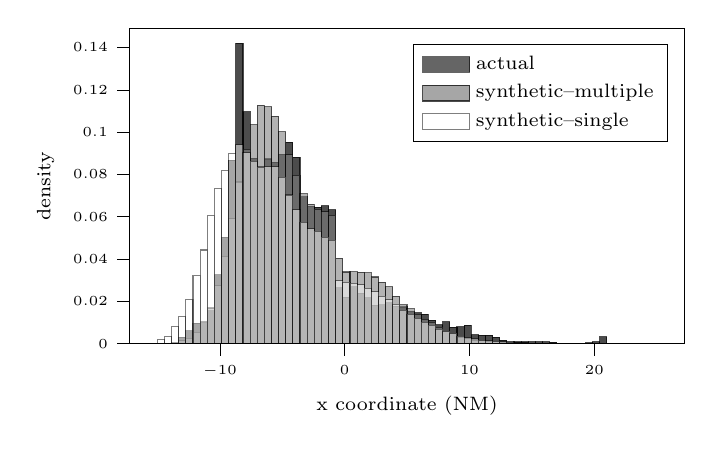
\begin{tikzpicture}

\begin{axis}[
legend cell align={left},
legend style={fill opacity=0.8, draw opacity=1, text opacity=1, draw=white!80!black},
width=3.4in,
height=2.2in,
tick align=outside,
tick pos=left,
x grid style={white!69.0196078431373!black},
xlabel={x coordinate (NM)},
xmin=-17.25, xmax=27.25,
xtick style={color=black},
y grid style={white!69.0196078431373!black},
ytick={0.00, 0.02, 0.04, 0.06, 0.08, 0.10, 0.12, 0.14},
ylabel={density},
ymin=0, ymax=0.149110572440798,
ytick style={color=black},
yticklabel style={/pgf/number format/.cd,fixed,precision=2},
tick label style={font=\tiny},
label style={font=\scriptsize},
legend entries={{actual},{synthetic--multiple},{synthetic--single}},
legend style={at={(0.97,0.95)}, anchor=north east, draw=black},
legend style={font=\scriptsize}
]

\addlegendimage{area legend, draw=black, fill=black, opacity=0.6}
\addlegendimage{area legend, draw=black, fill=white!50.1960784313725!black, opacity=0.7}
\addlegendimage{area legend, draw=black, fill=white, opacity=0.5}

\draw[draw=black,fill=black,opacity=0.7] (axis cs:-15,0) rectangle (axis cs:-14.4285714285714,0);
\draw[draw=black,fill=black,opacity=0.7] (axis cs:-14.4285714285714,0) rectangle (axis cs:-13.8571428571429,0);
\draw[draw=black,fill=black,opacity=0.7] (axis cs:-13.8571428571429,0) rectangle (axis cs:-13.2857142857143,0.000130523960469886);
\draw[draw=black,fill=black,opacity=0.7] (axis cs:-13.2857142857143,0) rectangle (axis cs:-12.7142857142857,0.00296942010068991);
\draw[draw=black,fill=black,opacity=0.7] (axis cs:-12.7142857142857,0) rectangle (axis cs:-12.1428571428571,0.00623251911243705);
\draw[draw=black,fill=black,opacity=0.7] (axis cs:-12.1428571428571,0) rectangle (axis cs:-11.5714285714286,0.00959351109453664);
\draw[draw=black,fill=black,opacity=0.7] (axis cs:-11.5714285714286,0) rectangle (axis cs:-11,0.0100829759462987);
\draw[draw=black,fill=black,opacity=0.7] (axis cs:-11,0) rectangle (axis cs:-10.4285714285714,0.0155976132761514);
\draw[draw=black,fill=black,opacity=0.7] (axis cs:-10.4285714285714,0) rectangle (axis cs:-9.85714285714286,0.0326962520977065);
\draw[draw=black,fill=black,opacity=0.7] (axis cs:-9.85714285714286,0) rectangle (axis cs:-9.28571428571429,0.0502517247809062);
\draw[draw=black,fill=black,opacity=0.7] (axis cs:-9.28571428571428,0) rectangle (axis cs:-8.71428571428571,0.086700540742122);
\draw[draw=black,fill=black,opacity=0.7] (axis cs:-8.71428571428572,0) rectangle (axis cs:-8.14285714285714,0.142010068991236);
\draw[draw=black,fill=black,opacity=0.7] (axis cs:-8.14285714285714,0) rectangle (axis cs:-7.57142857142857,0.109607495804587);
\draw[draw=black,fill=black,opacity=0.7] (axis cs:-7.57142857142857,0) rectangle (axis cs:-7,0.0877447324258809);
\draw[draw=black,fill=black,opacity=0.7] (axis cs:-7,0) rectangle (axis cs:-6.42857142857143,0.083796382621667);
\draw[draw=black,fill=black,opacity=0.7] (axis cs:-6.42857142857143,0) rectangle (axis cs:-5.85714285714286,0.0873205295543539);
\draw[draw=black,fill=black,opacity=0.7] (axis cs:-5.85714285714286,0) rectangle (axis cs:-5.28571428571429,0.0858521349990677);
\draw[draw=black,fill=black,opacity=0.7] (axis cs:-5.28571428571429,0) rectangle (axis cs:-4.71428571428572,0.089539436882342);
\draw[draw=black,fill=black,opacity=0.7] (axis cs:-4.71428571428572,0) rectangle (axis cs:-4.14285714285714,0.0951845981726646);
\draw[draw=black,fill=black,opacity=0.7] (axis cs:-4.14285714285714,0) rectangle (axis cs:-3.57142857142857,0.0881689352974082);
\draw[draw=black,fill=black,opacity=0.7] (axis cs:-3.57142857142857,0) rectangle (axis cs:-3,0.0695040089502142);
\draw[draw=black,fill=black,opacity=0.7] (axis cs:-3,0) rectangle (axis cs:-2.42857142857143,0.0648704083535335);
\draw[draw=black,fill=black,opacity=0.7] (axis cs:-2.42857142857143,0) rectangle (axis cs:-1.85714285714286,0.0644788364721238);
\draw[draw=black,fill=black,opacity=0.7] (axis cs:-1.85714285714286,0) rectangle (axis cs:-1.28571428571429,0.0651314562744733);
\draw[draw=black,fill=black,opacity=0.7] (axis cs:-1.28571428571429,0) rectangle (axis cs:-0.714285714285715,0.0633041208278949);
\draw[draw=black,fill=black,opacity=0.7] (axis cs:-0.714285714285715,0) rectangle (axis cs:-0.142857142857144,0.026365840014917);
\draw[draw=black,fill=black,opacity=0.7] (axis cs:-0.142857142857144,0) rectangle (axis cs:0.428571428571427,0.0220259183292933);
\draw[draw=black,fill=black,opacity=0.7] (axis cs:0.428571428571427,0) rectangle (axis cs:1,0.0270184598172664);
\draw[draw=black,fill=black,opacity=0.7] (axis cs:1,0) rectangle (axis cs:1.57142857142857,0.0239185157561067);
\draw[draw=black,fill=black,opacity=0.7] (axis cs:1.57142857142857,0) rectangle (axis cs:2.14285714285714,0.0218301323885884);
\draw[draw=black,fill=black,opacity=0.7] (axis cs:2.14285714285714,0) rectangle (axis cs:2.71428571428571,0.0182080924855492);
\draw[draw=black,fill=black,opacity=0.7] (axis cs:2.71428571428571,0) rectangle (axis cs:3.28571428571428,0.0184038784262539);
\draw[draw=black,fill=black,opacity=0.7] (axis cs:3.28571428571428,0) rectangle (axis cs:3.85714285714286,0.0192849151594256);
\draw[draw=black,fill=black,opacity=0.7] (axis cs:3.85714285714286,0) rectangle (axis cs:4.42857142857143,0.0177512586239046);
\draw[draw=black,fill=black,opacity=0.7] (axis cs:4.42857142857143,0) rectangle (axis cs:5,0.0173270557523774);
\draw[draw=black,fill=black,opacity=0.7] (axis cs:5,0) rectangle (axis cs:5.57142857142857,0.0152386723848593);
\draw[draw=black,fill=black,opacity=0.7] (axis cs:5.57142857142857,0) rectangle (axis cs:6.14285714285714,0.0147165765429796);
\draw[draw=black,fill=black,opacity=0.7] (axis cs:6.14285714285714,0) rectangle (axis cs:6.71428571428571,0.0138029088196905);
\draw[draw=black,fill=black,opacity=0.7] (axis cs:6.71428571428571,0) rectangle (axis cs:7.28571428571428,0.0111271676300578);
\draw[draw=black,fill=black,opacity=0.7] (axis cs:7.28571428571428,0) rectangle (axis cs:7.85714285714285,0.00894089129218724);
\draw[draw=black,fill=black,opacity=0.7] (axis cs:7.85714285714285,0) rectangle (axis cs:8.42857142857143,0.010311392877121);
\draw[draw=black,fill=black,opacity=0.7] (axis cs:8.42857142857143,0) rectangle (axis cs:9,0.00773354465784074);
\draw[draw=black,fill=black,opacity=0.7] (axis cs:9,0) rectangle (axis cs:9.57142857142857,0.00802722356889803);
\draw[draw=black,fill=black,opacity=0.7] (axis cs:9.57142857142857,0) rectangle (axis cs:10.1428571428571,0.00867984337124741);
\draw[draw=black,fill=black,opacity=0.7] (axis cs:10.1428571428571,0) rectangle (axis cs:10.7142857142857,0.00433992168562373);
\draw[draw=black,fill=black,opacity=0.7] (axis cs:10.7142857142857,0) rectangle (axis cs:11.2857142857143,0.00404624277456646);
\draw[draw=black,fill=black,opacity=0.7] (axis cs:11.2857142857143,0) rectangle (axis cs:11.8571428571429,0.00388308782397913);
\draw[draw=black,fill=black,opacity=0.7] (axis cs:11.8571428571429,0) rectangle (axis cs:12.4285714285714,0.00306731307104232);
\draw[draw=black,fill=black,opacity=0.7] (axis cs:12.4285714285714,0) rectangle (axis cs:13,0.00166418049599105);
\draw[draw=black,fill=black,opacity=0.7] (axis cs:13,0) rectangle (axis cs:13.5714285714286,0.000848405743054264);
\draw[draw=black,fill=black,opacity=0.7] (axis cs:13.5714285714286,0) rectangle (axis cs:14.1428571428571,0.00088103673317173);
\draw[draw=black,fill=black,opacity=0.7] (axis cs:14.1428571428571,0) rectangle (axis cs:14.7142857142857,0.000913667723289207);
\draw[draw=black,fill=black,opacity=0.7] (axis cs:14.7142857142857,0) rectangle (axis cs:15.2857142857143,0.000913667723289201);
\draw[draw=black,fill=black,opacity=0.7] (axis cs:15.2857142857143,0) rectangle (axis cs:15.8571428571429,0.000946298713406679);
\draw[draw=black,fill=black,opacity=0.7] (axis cs:15.8571428571429,0) rectangle (axis cs:16.4285714285714,0.000848405743054258);
\draw[draw=black,fill=black,opacity=0.7] (axis cs:16.4285714285714,0) rectangle (axis cs:17,0.000587357822114487);
\draw[draw=black,fill=black,opacity=0.7] (axis cs:17,0) rectangle (axis cs:17.5714285714286,0.000261047920939773);
\draw[draw=black,fill=black,opacity=0.7] (axis cs:17.5714285714286,0) rectangle (axis cs:18.1428571428571,0.000261047920939773);
\draw[draw=black,fill=black,opacity=0.7] (axis cs:18.1428571428571,0) rectangle (axis cs:18.7142857142857,0.000228416930822299);
\draw[draw=black,fill=black,opacity=0.7] (axis cs:18.7142857142857,0) rectangle (axis cs:19.2857142857143,0.000261047920939773);
\draw[draw=black,fill=black,opacity=0.7] (axis cs:19.2857142857143,0) rectangle (axis cs:19.8571428571429,0.000358940891292188);
\draw[draw=black,fill=black,opacity=0.7] (axis cs:19.8571428571429,0) rectangle (axis cs:20.4285714285714,0.000848405743054264);
\draw[draw=black,fill=black,opacity=0.7] (axis cs:20.4285714285714,0) rectangle (axis cs:21,0.00336099198209954);
\draw[draw=black,fill=black,opacity=0.7] (axis cs:21,0) rectangle (axis cs:21.5714285714286,0);
\draw[draw=black,fill=black,opacity=0.7] (axis cs:21.5714285714286,0) rectangle (axis cs:22.1428571428571,0);
\draw[draw=black,fill=black,opacity=0.7] (axis cs:22.1428571428571,0) rectangle (axis cs:22.7142857142857,0);
\draw[draw=black,fill=black,opacity=0.7] (axis cs:22.7142857142857,0) rectangle (axis cs:23.2857142857143,0);
\draw[draw=black,fill=black,opacity=0.7] (axis cs:23.2857142857143,0) rectangle (axis cs:23.8571428571429,0);
\draw[draw=black,fill=black,opacity=0.7] (axis cs:23.8571428571429,0) rectangle (axis cs:24.4285714285714,0);
\draw[draw=black,fill=black,opacity=0.7] (axis cs:24.4285714285714,0) rectangle (axis cs:25,0);
\draw[draw=black,fill=white!50.1960784313725!black,opacity=0.6] (axis cs:-15,0) rectangle (axis cs:-14.4285714285714,0.000135501896527005);
\draw[draw=black,fill=white!50.1960784313725!black,opacity=0.6] (axis cs:-14.4285714285714,0) rectangle (axis cs:-13.8571428571429,0.000290236320303005);
\draw[draw=black,fill=white!50.1960784313725!black,opacity=0.6] (axis cs:-13.8571428571429,0) rectangle (axis cs:-13.2857142857143,0.000654780132249851);
\draw[draw=black,fill=white!50.1960784313725!black,opacity=0.6] (axis cs:-13.2857142857143,0) rectangle (axis cs:-12.7142857142857,0.00147915618660447);
\draw[draw=black,fill=white!50.1960784313725!black,opacity=0.6] (axis cs:-12.7142857142857,0) rectangle (axis cs:-12.1428571428571,0.0024818702209043);
\draw[draw=black,fill=white!50.1960784313725!black,opacity=0.6] (axis cs:-12.1428571428571,0) rectangle (axis cs:-11.5714285714286,0.00530642910915434);
\draw[draw=black,fill=white!50.1960784313725!black,opacity=0.6] (axis cs:-11.5714285714286,0) rectangle (axis cs:-11,0.0103165024575174);
\draw[draw=black,fill=white!50.1960784313725!black,opacity=0.6] (axis cs:-11,0) rectangle (axis cs:-10.4285714285714,0.0168852847188329);
\draw[draw=black,fill=white!50.1960784313725!black,opacity=0.6] (axis cs:-10.4285714285714,0) rectangle (axis cs:-9.85714285714286,0.0273145597224921);
\draw[draw=black,fill=white!50.1960784313725!black,opacity=0.6] (axis cs:-9.85714285714286,0) rectangle (axis cs:-9.28571428571429,0.041218802717731);
\draw[draw=black,fill=white!50.1960784313725!black,opacity=0.6] (axis cs:-9.28571428571428,0) rectangle (axis cs:-8.71428571428571,0.0590316197734359);
\draw[draw=black,fill=white!50.1960784313725!black,opacity=0.6] (axis cs:-8.71428571428572,0) rectangle (axis cs:-8.14285714285714,0.0764204470238786);
\draw[draw=black,fill=white!50.1960784313725!black,opacity=0.6] (axis cs:-8.14285714285714,0) rectangle (axis cs:-7.57142857142857,0.0919515869832259);
\draw[draw=black,fill=white!50.1960784313725!black,opacity=0.6] (axis cs:-7.57142857142857,0) rectangle (axis cs:-7,0.10349285174419);
\draw[draw=black,fill=white!50.1960784313725!black,opacity=0.6] (axis cs:-7,0) rectangle (axis cs:-6.42857142857143,0.112663270418825);
\draw[draw=black,fill=white!50.1960784313725!black,opacity=0.6] (axis cs:-6.42857142857143,0) rectangle (axis cs:-5.85714285714286,0.112004993463439);
\draw[draw=black,fill=white!50.1960784313725!black,opacity=0.6] (axis cs:-5.85714285714286,0) rectangle (axis cs:-5.28571428571429,0.107521191997071);
\draw[draw=black,fill=white!50.1960784313725!black,opacity=0.6] (axis cs:-5.28571428571429,0) rectangle (axis cs:-4.71428571428572,0.100177863411091);
\draw[draw=black,fill=white!50.1960784313725!black,opacity=0.6] (axis cs:-4.71428571428572,0) rectangle (axis cs:-4.14285714285714,0.089344705335203);
\draw[draw=black,fill=white!50.1960784313725!black,opacity=0.6] (axis cs:-4.14285714285714,0) rectangle (axis cs:-3.57142857142857,0.0795841977563384);
\draw[draw=black,fill=white!50.1960784313725!black,opacity=0.6] (axis cs:-3.57142857142857,0) rectangle (axis cs:-3,0.0708211589770691);
\draw[draw=black,fill=white!50.1960784313725!black,opacity=0.6] (axis cs:-3,0) rectangle (axis cs:-2.42857142857143,0.065920361351712);
\draw[draw=black,fill=white!50.1960784313725!black,opacity=0.6] (axis cs:-2.42857142857143,0) rectangle (axis cs:-1.85714285714286,0.0635294085323484);
\draw[draw=black,fill=white!50.1960784313725!black,opacity=0.6] (axis cs:-1.85714285714286,0) rectangle (axis cs:-1.28571428571429,0.0622967783768447);
\draw[draw=black,fill=white!50.1960784313725!black,opacity=0.6] (axis cs:-1.28571428571429,0) rectangle (axis cs:-0.714285714285715,0.0606751266474408);
\draw[draw=black,fill=white!50.1960784313725!black,opacity=0.6] (axis cs:-0.714285714285715,0) rectangle (axis cs:-0.142857142857144,0.0402694152362579);
\draw[draw=black,fill=white!50.1960784313725!black,opacity=0.6] (axis cs:-0.142857142857144,0) rectangle (axis cs:0.428571428571427,0.0338842161895918);
\draw[draw=black,fill=white!50.1960784313725!black,opacity=0.6] (axis cs:0.428571428571427,0) rectangle (axis cs:1,0.0339690141506441);
\draw[draw=black,fill=white!50.1960784313725!black,opacity=0.6] (axis cs:1,0) rectangle (axis cs:1.57142857142857,0.033752211116201);
\draw[draw=black,fill=white!50.1960784313725!black,opacity=0.6] (axis cs:1.57142857142857,0) rectangle (axis cs:2.14285714285714,0.033561634255279);
\draw[draw=black,fill=white!50.1960784313725!black,opacity=0.6] (axis cs:2.14285714285714,0) rectangle (axis cs:2.71428571428571,0.0315299800131582);
\draw[draw=black,fill=white!50.1960784313725!black,opacity=0.6] (axis cs:2.71428571428571,0) rectangle (axis cs:3.28571428571428,0.0289475761270885);
\draw[draw=black,fill=white!50.1960784313725!black,opacity=0.6] (axis cs:3.28571428571428,0) rectangle (axis cs:3.85714285714286,0.0269753678782825);
\draw[draw=black,fill=white!50.1960784313725!black,opacity=0.6] (axis cs:3.85714285714286,0) rectangle (axis cs:4.42857142857143,0.0224635918268254);
\draw[draw=black,fill=white!50.1960784313725!black,opacity=0.6] (axis cs:4.42857142857143,0) rectangle (axis cs:5,0.0185139300945091);
\draw[draw=black,fill=white!50.1960784313725!black,opacity=0.6] (axis cs:5,0) rectangle (axis cs:5.57142857142857,0.0165705706365767);
\draw[draw=black,fill=white!50.1960784313725!black,opacity=0.6] (axis cs:5.57142857142857,0) rectangle (axis cs:6.14285714285714,0.013870148969661);
\draw[draw=black,fill=white!50.1960784313725!black,opacity=0.6] (axis cs:6.14285714285714,0) rectangle (axis cs:6.71428571428571,0.011546509995669);
\draw[draw=black,fill=white!50.1960784313725!black,opacity=0.6] (axis cs:6.71428571428571,0) rectangle (axis cs:7.28571428571428,0.0100962025999379);
\draw[draw=black,fill=white!50.1960784313725!black,opacity=0.6] (axis cs:7.28571428571428,0) rectangle (axis cs:7.85714285714285,0.00784250008866947);
\draw[draw=black,fill=white!50.1960784313725!black,opacity=0.6] (axis cs:7.85714285714285,0) rectangle (axis cs:8.42857142857143,0.00567097292110116);
\draw[draw=black,fill=white!50.1960784313725!black,opacity=0.6] (axis cs:8.42857142857143,0) rectangle (axis cs:9,0.00465252318268851);
\draw[draw=black,fill=white!50.1960784313725!black,opacity=0.6] (axis cs:9,0) rectangle (axis cs:9.57142857142857,0.00306496547886246);
\draw[draw=black,fill=white!50.1960784313725!black,opacity=0.6] (axis cs:9.57142857142857,0) rectangle (axis cs:10.1428571428571,0.00226768980381323);
\draw[draw=black,fill=white!50.1960784313725!black,opacity=0.6] (axis cs:10.1428571428571,0) rectangle (axis cs:10.7142857142857,0.00175890203749894);
\draw[draw=black,fill=white!50.1960784313725!black,opacity=0.6] (axis cs:10.7142857142857,0) rectangle (axis cs:11.2857142857143,0.00147565936346829);
\draw[draw=black,fill=white!50.1960784313725!black,opacity=0.6] (axis cs:11.2857142857143,0) rectangle (axis cs:11.8571428571429,0.00124574324226441);
\draw[draw=black,fill=white!50.1960784313725!black,opacity=0.6] (axis cs:11.8571428571429,0) rectangle (axis cs:12.4285714285714,0.000868960549340921);
\draw[draw=black,fill=white!50.1960784313725!black,opacity=0.6] (axis cs:12.4285714285714,0) rectangle (axis cs:13,0.000679257894203115);
\draw[draw=black,fill=white!50.1960784313725!black,opacity=0.6] (axis cs:13,0) rectangle (axis cs:13.5714285714286,0.000509661972098351);
\draw[draw=black,fill=white!50.1960784313725!black,opacity=0.6] (axis cs:13.5714285714286,0) rectangle (axis cs:14.1428571428571,0.000397763631740563);
\draw[draw=black,fill=white!50.1960784313725!black,opacity=0.6] (axis cs:14.1428571428571,0) rectangle (axis cs:14.7142857142857,0.000335695021073356);
\draw[draw=black,fill=white!50.1960784313725!black,opacity=0.6] (axis cs:14.7142857142857,0) rectangle (axis cs:15.2857142857143,0.000230790326987931);
\draw[draw=black,fill=white!50.1960784313725!black,opacity=0.6] (axis cs:15.2857142857143,0) rectangle (axis cs:15.8571428571429,0.000187080037785672);
\draw[draw=black,fill=white!50.1960784313725!black,opacity=0.6] (axis cs:15.8571428571429,0) rectangle (axis cs:16.4285714285714,0.000145992365935547);
\draw[draw=black,fill=white!50.1960784313725!black,opacity=0.6] (axis cs:16.4285714285714,0) rectangle (axis cs:17,9.26658131087904e-05);
\draw[draw=black,fill=white!50.1960784313725!black,opacity=0.6] (axis cs:17,0) rectangle (axis cs:17.5714285714286,9.2665813108791e-05);
\draw[draw=black,fill=white!50.1960784313725!black,opacity=0.6] (axis cs:17.5714285714286,0) rectangle (axis cs:18.1428571428571,8.56721668364294e-05);
\draw[draw=black,fill=white!50.1960784313725!black,opacity=0.6] (axis cs:18.1428571428571,0) rectangle (axis cs:18.7142857142857,8.65463726204735e-05);
\draw[draw=black,fill=white!50.1960784313725!black,opacity=0.6] (axis cs:18.7142857142857,0) rectangle (axis cs:19.2857142857143,8.56721668364294e-05);
\draw[draw=black,fill=white!50.1960784313725!black,opacity=0.6] (axis cs:19.2857142857143,0) rectangle (axis cs:19.8571428571429,9.79110478130622e-05);
\draw[draw=black,fill=white!50.1960784313725!black,opacity=0.6] (axis cs:19.8571428571429,0) rectangle (axis cs:20.4285714285714,7.16848742917062e-05);
\draw[draw=black,fill=white!50.1960784313725!black,opacity=0.6] (axis cs:20.4285714285714,0) rectangle (axis cs:21,6.90622569395698e-05);
\draw[draw=black,fill=white!50.1960784313725!black,opacity=0.6] (axis cs:21,0) rectangle (axis cs:21.5714285714286,7.25590800757514e-05);
\draw[draw=black,fill=white!50.1960784313725!black,opacity=0.6] (axis cs:21.5714285714286,0) rectangle (axis cs:22.1428571428571,7.16848742917062e-05);
\draw[draw=black,fill=white!50.1960784313725!black,opacity=0.6] (axis cs:22.1428571428571,0) rectangle (axis cs:22.7142857142857,7.51816974278861e-05);
\draw[draw=black,fill=white!50.1960784313725!black,opacity=0.6] (axis cs:22.7142857142857,0) rectangle (axis cs:23.2857142857143,7.5181697427887e-05);
\draw[draw=black,fill=white!50.1960784313725!black,opacity=0.6] (axis cs:23.2857142857143,0) rectangle (axis cs:23.8571428571429,7.78043147800226e-05);
\draw[draw=black,fill=white!50.1960784313725!black,opacity=0.6] (axis cs:23.8571428571429,0) rectangle (axis cs:24.4285714285714,8.13011379162034e-05);
\draw[draw=black,fill=white!50.1960784313725!black,opacity=0.6] (axis cs:24.4285714285714,0) rectangle (axis cs:25,6.11944048831631e-05);
\draw[draw=black,fill=white,opacity=0.5] (axis cs:-15,0) rectangle (axis cs:-14.4285714285714,0.00190133249248095);
\draw[draw=black,fill=white,opacity=0.5] (axis cs:-14.4285714285714,0) rectangle (axis cs:-13.8571428571429,0.00357741659345743);
\draw[draw=black,fill=white,opacity=0.5] (axis cs:-13.8571428571429,0) rectangle (axis cs:-13.2857142857143,0.00797123565393978);
\draw[draw=black,fill=white,opacity=0.5] (axis cs:-13.2857142857143,0) rectangle (axis cs:-12.7142857142857,0.0129945698697185);
\draw[draw=black,fill=white,opacity=0.5] (axis cs:-12.7142857142857,0) rectangle (axis cs:-12.1428571428571,0.0208812144246652);
\draw[draw=black,fill=white,opacity=0.5] (axis cs:-12.1428571428571,0) rectangle (axis cs:-11.5714285714286,0.0323324885464776);
\draw[draw=black,fill=white,opacity=0.5] (axis cs:-11.5714285714286,0) rectangle (axis cs:-11,0.0443060635236999);
\draw[draw=black,fill=white,opacity=0.5] (axis cs:-11,0) rectangle (axis cs:-10.4285714285714,0.0607836227135813);
\draw[draw=black,fill=white,opacity=0.5] (axis cs:-10.4285714285714,0) rectangle (axis cs:-9.85714285714286,0.0734506479790597);
\draw[draw=black,fill=white,opacity=0.5] (axis cs:-9.85714285714286,0) rectangle (axis cs:-9.28571428571429,0.081902872556343);
\draw[draw=black,fill=white,opacity=0.5] (axis cs:-9.28571428571428,0) rectangle (axis cs:-8.71428571428571,0.0898288618084959);
\draw[draw=black,fill=white,opacity=0.5] (axis cs:-8.71428571428572,0) rectangle (axis cs:-8.14285714285714,0.0941105484819408);
\draw[draw=black,fill=white,opacity=0.5] (axis cs:-8.14285714285714,0) rectangle (axis cs:-7.57142857142857,0.0903167360538507);
\draw[draw=black,fill=white,opacity=0.5] (axis cs:-7.57142857142857,0) rectangle (axis cs:-7,0.0861304602711298);
\draw[draw=black,fill=white,opacity=0.5] (axis cs:-7,0) rectangle (axis cs:-6.42857142857143,0.0833527246483849);
\draw[draw=black,fill=white,opacity=0.5] (axis cs:-6.42857142857143,0) rectangle (axis cs:-5.85714285714286,0.08358190750961);
\draw[draw=black,fill=white,opacity=0.5] (axis cs:-5.85714285714286,0) rectangle (axis cs:-5.28571428571429,0.0835789566573195);
\draw[draw=black,fill=white,opacity=0.5] (axis cs:-5.28571428571429,0) rectangle (axis cs:-4.71428571428572,0.0786470988625448);
\draw[draw=black,fill=white,opacity=0.5] (axis cs:-4.71428571428572,0) rectangle (axis cs:-4.14285714285714,0.0702676619750926);
\draw[draw=black,fill=white,opacity=0.5] (axis cs:-4.14285714285714,0) rectangle (axis cs:-3.57142857142857,0.0633951269906309);
\draw[draw=black,fill=white,opacity=0.5] (axis cs:-3.57142857142857,0) rectangle (axis cs:-3,0.0574678483565437);
\draw[draw=black,fill=white,opacity=0.5] (axis cs:-3,0) rectangle (axis cs:-2.42857142857143,0.0542681408562643);
\draw[draw=black,fill=white,opacity=0.5] (axis cs:-2.42857142857143,0) rectangle (axis cs:-1.85714285714286,0.0532018995619811);
\draw[draw=black,fill=white,opacity=0.5] (axis cs:-1.85714285714286,0) rectangle (axis cs:-1.28571428571429,0.0502461291843788);
\draw[draw=black,fill=white,opacity=0.5] (axis cs:-1.28571428571429,0) rectangle (axis cs:-0.714285714285715,0.0488543105207159);
\draw[draw=black,fill=white,opacity=0.5] (axis cs:-0.714285714285715,0) rectangle (axis cs:-0.142857142857144,0.0297180334171376);
\draw[draw=black,fill=white,opacity=0.5] (axis cs:-0.142857142857144,0) rectangle (axis cs:0.428571428571427,0.0290904854967015);
\draw[draw=black,fill=white,opacity=0.5] (axis cs:0.428571428571427,0) rectangle (axis cs:1,0.0284570358716845);
\draw[draw=black,fill=white,opacity=0.5] (axis cs:1,0) rectangle (axis cs:1.57142857142857,0.0278452258301311);
\draw[draw=black,fill=white,opacity=0.5] (axis cs:1.57142857142857,0) rectangle (axis cs:2.14285714285714,0.0261671744942941);
\draw[draw=black,fill=white,opacity=0.5] (axis cs:2.14285714285714,0) rectangle (axis cs:2.71428571428571,0.0244645327227037);
\draw[draw=black,fill=white,opacity=0.5] (axis cs:2.71428571428571,0) rectangle (axis cs:3.28571428571428,0.0224943470101121);
\draw[draw=black,fill=white,opacity=0.5] (axis cs:3.28571428571428,0) rectangle (axis cs:3.85714285714286,0.0207907216210914);
\draw[draw=black,fill=white,opacity=0.5] (axis cs:3.85714285714286,0) rectangle (axis cs:4.42857142857143,0.0186513537105141);
\draw[draw=black,fill=white,opacity=0.5] (axis cs:4.42857142857143,0) rectangle (axis cs:5,0.0157841089016253);
\draw[draw=black,fill=white,opacity=0.5] (axis cs:5,0) rectangle (axis cs:5.57142857142857,0.0138237593633354);
\draw[draw=black,fill=white,opacity=0.5] (axis cs:5.57142857142857,0) rectangle (axis cs:6.14285714285714,0.0120001326478363);
\draw[draw=black,fill=white,opacity=0.5] (axis cs:6.14285714285714,0) rectangle (axis cs:6.71428571428571,0.0100889639810539);
\draw[draw=black,fill=white,opacity=0.5] (axis cs:6.71428571428571,0) rectangle (axis cs:7.28571428571428,0.00879058897325514);
\draw[draw=black,fill=white,opacity=0.5] (axis cs:7.28571428571428,0) rectangle (axis cs:7.85714285714285,0.00671613981306775);
\draw[draw=black,fill=white,opacity=0.5] (axis cs:7.85714285714285,0) rectangle (axis cs:8.42857142857143,0.00581612986447999);
\draw[draw=black,fill=white,opacity=0.5] (axis cs:8.42857142857143,0) rectangle (axis cs:9,0.00495153014337768);
\draw[draw=black,fill=white,opacity=0.5] (axis cs:9,0) rectangle (axis cs:9.57142857142857,0.00354298998340217);
\draw[draw=black,fill=white,opacity=0.5] (axis cs:9.57142857142857,0) rectangle (axis cs:10.1428571428571,0.0028721628960395);
\draw[draw=black,fill=white,opacity=0.5] (axis cs:10.1428571428571,0) rectangle (axis cs:10.7142857142857,0.00242461696532103);
\draw[draw=black,fill=white,opacity=0.5] (axis cs:10.7142857142857,0) rectangle (axis cs:11.2857142857143,0.00169083836242873);
\draw[draw=black,fill=white,opacity=0.5] (axis cs:11.2857142857143,0) rectangle (axis cs:11.8571428571429,0.00137214631505997);
\draw[draw=black,fill=white,opacity=0.5] (axis cs:11.8571428571429,0) rectangle (axis cs:12.4285714285714,0.00107017576400376);
\draw[draw=black,fill=white,opacity=0.5] (axis cs:12.4285714285714,0) rectangle (axis cs:13,0.000835091198197786);
\draw[draw=black,fill=white,opacity=0.5] (axis cs:13,0) rectangle (axis cs:13.5714285714286,0.000636400477307386);
\draw[draw=black,fill=white,opacity=0.5] (axis cs:13.5714285714286,0) rectangle (axis cs:14.1428571428571,0.000489841480214956);
\draw[draw=black,fill=white,opacity=0.5] (axis cs:14.1428571428571,0) rectangle (axis cs:14.7142857142857,0.000353118657424037);
\draw[draw=black,fill=white,opacity=0.5] (axis cs:14.7142857142857,0) rectangle (axis cs:15.2857142857143,0.000231150096085371);
\draw[draw=black,fill=white,opacity=0.5] (axis cs:15.2857142857143,0) rectangle (axis cs:15.8571428571429,0.000197707103460254);
\draw[draw=black,fill=white,opacity=0.5] (axis cs:15.8571428571429,0) rectangle (axis cs:16.4285714285714,0.000150493466813029);
\draw[draw=black,fill=white,opacity=0.5] (axis cs:16.4285714285714,0) rectangle (axis cs:17,0.000119017709048212);
\draw[draw=black,fill=white,opacity=0.5] (axis cs:17,0) rectangle (axis cs:17.5714285714286,9.54108907246004e-05);
\draw[draw=black,fill=white,opacity=0.5] (axis cs:17.5714285714286,0) rectangle (axis cs:18.1428571428571,7.7705776981891e-05);
\draw[draw=black,fill=white,opacity=0.5] (axis cs:18.1428571428571,0) rectangle (axis cs:18.7142857142857,7.08204549708365e-05);
\draw[draw=black,fill=white,opacity=0.5] (axis cs:18.7142857142857,0) rectangle (axis cs:19.2857142857143,6.59023678200848e-05);
\draw[draw=black,fill=white,opacity=0.5] (axis cs:19.2857142857143,0) rectangle (axis cs:19.8571428571429,6.49187503899343e-05);
\draw[draw=black,fill=white,opacity=0.5] (axis cs:19.8571428571429,0) rectangle (axis cs:20.4285714285714,7.27876898311384e-05);
\draw[draw=black,fill=white,opacity=0.5] (axis cs:20.4285714285714,0) rectangle (axis cs:21,7.96730118421911e-05);
\draw[draw=black,fill=white,opacity=0.5] (axis cs:21,0) rectangle (axis cs:21.5714285714286,8.55747164230952e-05);
\draw[draw=black,fill=white,opacity=0.5] (axis cs:21.5714285714286,0) rectangle (axis cs:22.1428571428571,6.39351329597838e-05);
\draw[draw=black,fill=white,opacity=0.5] (axis cs:22.1428571428571,0) rectangle (axis cs:22.7142857142857,6.49187503899335e-05);
\draw[draw=black,fill=white,opacity=0.5] (axis cs:22.7142857142857,0) rectangle (axis cs:23.2857142857143,6.39351329597838e-05);
\draw[draw=black,fill=white,opacity=0.5] (axis cs:23.2857142857143,0) rectangle (axis cs:23.8571428571429,6.59023678200848e-05);
\draw[draw=black,fill=white,opacity=0.5] (axis cs:23.8571428571429,0) rectangle (axis cs:24.4285714285714,7.573854212159e-05);
\draw[draw=black,fill=white,opacity=0.5] (axis cs:24.4285714285714,0) rectangle (axis cs:25,6.68859852502345e-05);
\end{axis}

\end{tikzpicture}}
    \hspace*{1em}%
    \subfigure[yNorth. $D_{JS}$: 0.0446 (multiple), 0.0166 (single)]{
        \label{fig:hist_y_coords}
        % This file was created by tikzplotlib v0.9.2.
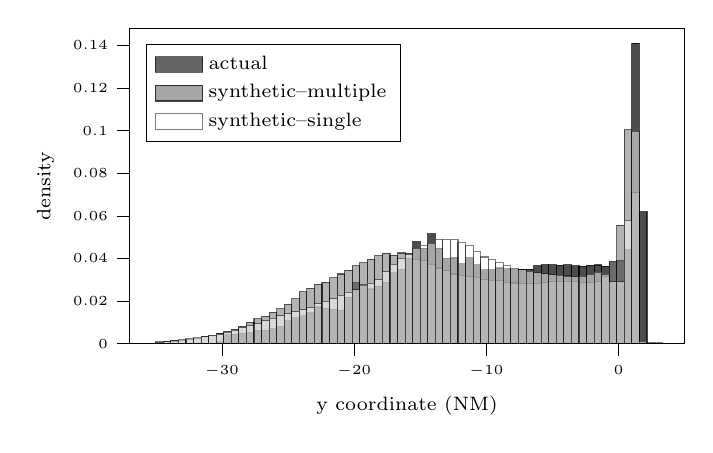
\begin{tikzpicture}

\begin{axis}[
legend cell align={left},
legend style={fill opacity=0.8, draw opacity=1, text opacity=1, draw=white!80!black},
width=3.4in,
height=2.2in,
tick align=outside,
tick pos=left,
x grid style={white!69.0196078431373!black},
xlabel={y coordinate (NM)},
xmin=-37, xmax=5,
xtick style={color=black},
y grid style={white!69.0196078431373!black},
ytick={0.00, 0.02, 0.04, 0.06, 0.08, 0.10, 0.12, 0.14},
ylabel={density},
ymin=0, ymax=0.148014171172852,
ytick style={color=black},
yticklabel style={/pgf/number format/.cd,fixed,precision=2},
tick label style={font=\tiny},
label style={font=\scriptsize},
legend entries={{actual},{synthetic--multiple}, {synthetic--single}},
legend style={at={(0.03,0.95)}, anchor=north west, draw=black},
legend style={font=\scriptsize}
]

\addlegendimage{area legend, draw=black, fill=black, opacity=0.6}
\addlegendimage{area legend, draw=black, fill=white!50.1960784313725!black, opacity=0.7}
\addlegendimage{area legend, draw=black, fill=white, opacity=0.5}

\draw[draw=black,fill=black,opacity=0.7] (axis cs:-35,0) rectangle (axis cs:-34.4285714285714,0);
\draw[draw=black,fill=black,opacity=0.7] (axis cs:-34.4285714285714,0) rectangle (axis cs:-33.8571428571429,0);
\draw[draw=black,fill=black,opacity=0.7] (axis cs:-33.8571428571429,0) rectangle (axis cs:-33.2857142857143,0);
\draw[draw=black,fill=black,opacity=0.7] (axis cs:-33.2857142857143,0) rectangle (axis cs:-32.7142857142857,0);
\draw[draw=black,fill=black,opacity=0.7] (axis cs:-32.7142857142857,0) rectangle (axis cs:-32.1428571428571,0);
\draw[draw=black,fill=black,opacity=0.7] (axis cs:-32.1428571428572,0) rectangle (axis cs:-31.5714285714286,0);
\draw[draw=black,fill=black,opacity=0.7] (axis cs:-31.5714285714286,0) rectangle (axis cs:-31,0);
\draw[draw=black,fill=black,opacity=0.7] (axis cs:-31,0) rectangle (axis cs:-30.4285714285714,0);
\draw[draw=black,fill=black,opacity=0.7] (axis cs:-30.4285714285714,0) rectangle (axis cs:-29.8571428571429,0.00088103673317173);
\draw[draw=black,fill=black,opacity=0.7] (axis cs:-29.8571428571429,0) rectangle (axis cs:-29.2857142857143,0.00411150475480141);
\draw[draw=black,fill=black,opacity=0.7] (axis cs:-29.2857142857143,0) rectangle (axis cs:-28.7142857142857,0.00443781465597615);
\draw[draw=black,fill=black,opacity=0.7] (axis cs:-28.7142857142857,0) rectangle (axis cs:-28.1428571428571,0.00479675554726831);
\draw[draw=black,fill=black,opacity=0.7] (axis cs:-28.1428571428571,0) rectangle (axis cs:-27.5714285714286,0.005188327428678);
\draw[draw=black,fill=black,opacity=0.7] (axis cs:-27.5714285714286,0) rectangle (axis cs:-27,0.00597147119149728);
\draw[draw=black,fill=black,opacity=0.7] (axis cs:-27,0) rectangle (axis cs:-26.4285714285714,0.00636304307290698);
\draw[draw=black,fill=black,opacity=0.7] (axis cs:-26.4285714285714,0) rectangle (axis cs:-25.8571428571429,0.00695040089502142);
\draw[draw=black,fill=black,opacity=0.7] (axis cs:-25.8571428571429,0) rectangle (axis cs:-25.2857142857143,0.0081251165392504);
\draw[draw=black,fill=black,opacity=0.7] (axis cs:-25.2857142857143,0) rectangle (axis cs:-24.7142857142857,0.0108008577288831);
\draw[draw=black,fill=black,opacity=0.7] (axis cs:-24.7142857142857,0) rectangle (axis cs:-24.1428571428571,0.0122366212940519);
\draw[draw=black,fill=black,opacity=0.7] (axis cs:-24.1428571428571,0) rectangle (axis cs:-23.5714285714286,0.0130523960469886);
\draw[draw=black,fill=black,opacity=0.7] (axis cs:-23.5714285714286,0) rectangle (axis cs:-23,0.0144228976319224);
\draw[draw=black,fill=black,opacity=0.7] (axis cs:-23,0) rectangle (axis cs:-22.4285714285714,0.0171965317919076);
\draw[draw=black,fill=black,opacity=0.7] (axis cs:-22.4285714285714,0) rectangle (axis cs:-21.8571428571429,0.0166744359500279);
\draw[draw=black,fill=black,opacity=0.7] (axis cs:-21.8571428571429,0) rectangle (axis cs:-21.2857142857143,0.0162176020883833);
\draw[draw=black,fill=black,opacity=0.7] (axis cs:-21.2857142857143,0) rectangle (axis cs:-20.7142857142857,0.0155976132761515);
\draw[draw=black,fill=black,opacity=0.7] (axis cs:-20.7142857142857,0) rectangle (axis cs:-20.1428571428571,0.0217322394182361);
\draw[draw=black,fill=black,opacity=0.7] (axis cs:-20.1428571428571,0) rectangle (axis cs:-19.5714285714286,0.0288784262539623);
\draw[draw=black,fill=black,opacity=0.7] (axis cs:-19.5714285714286,0) rectangle (axis cs:-19,0.0267574118963266);
\draw[draw=black,fill=black,opacity=0.7] (axis cs:-19,0) rectangle (axis cs:-18.4285714285714,0.0256479582323327);
\draw[draw=black,fill=black,opacity=0.7] (axis cs:-18.4285714285714,0) rectangle (axis cs:-17.8571428571429,0.026920566846914);
\draw[draw=black,fill=black,opacity=0.7] (axis cs:-17.8571428571429,0) rectangle (axis cs:-17.2857142857143,0.02878053328361);
\draw[draw=black,fill=black,opacity=0.7] (axis cs:-17.2857142857143,0) rectangle (axis cs:-16.7142857142857,0.0332509789297034);
\draw[draw=black,fill=black,opacity=0.7] (axis cs:-16.7142857142857,0) rectangle (axis cs:-16.1428571428571,0.0348172664553421);
\draw[draw=black,fill=black,opacity=0.7] (axis cs:-16.1428571428571,0) rectangle (axis cs:-15.5714285714286,0.0400055938840203);
\draw[draw=black,fill=black,opacity=0.7] (axis cs:-15.5714285714286,0) rectangle (axis cs:-15,0.0478044005220957);
\draw[draw=black,fill=black,opacity=0.7] (axis cs:-15,0) rectangle (axis cs:-14.4285714285714,0.0447044564609362);
\draw[draw=black,fill=black,opacity=0.7] (axis cs:-14.4285714285714,0) rectangle (axis cs:-13.8571428571429,0.0515569643856049);
\draw[draw=black,fill=black,opacity=0.7] (axis cs:-13.8571428571429,0) rectangle (axis cs:-13.2857142857143,0.0447697184411711);
\draw[draw=black,fill=black,opacity=0.7] (axis cs:-13.2857142857143,0) rectangle (axis cs:-12.7142857142857,0.0401034868543724);
\draw[draw=black,fill=black,opacity=0.7] (axis cs:-12.7142857142857,0) rectangle (axis cs:-12.1428571428571,0.0402013798247251);
\draw[draw=black,fill=black,opacity=0.7] (axis cs:-12.1428571428571,0) rectangle (axis cs:-11.5714285714286,0.0375909006153271);
\draw[draw=black,fill=black,opacity=0.7] (axis cs:-11.5714285714286,0) rectangle (axis cs:-11,0.0402666418049598);
\draw[draw=black,fill=black,opacity=0.7] (axis cs:-11,0) rectangle (axis cs:-10.4285714285714,0.0369709118030954);
\draw[draw=black,fill=black,opacity=0.7] (axis cs:-10.4285714285714,0) rectangle (axis cs:-9.85714285714286,0.0346214805146372);
\draw[draw=black,fill=black,opacity=0.7] (axis cs:-9.85714285714286,0) rectangle (axis cs:-9.28571428571429,0.0346867424948724);
\draw[draw=black,fill=black,opacity=0.7] (axis cs:-9.28571428571429,0) rectangle (axis cs:-8.71428571428571,0.0355351482379264);
\draw[draw=black,fill=black,opacity=0.7] (axis cs:-8.71428571428572,0) rectangle (axis cs:-8.14285714285715,0.0352088383367519);
\draw[draw=black,fill=black,opacity=0.7] (axis cs:-8.14285714285715,0) rectangle (axis cs:-7.57142857142857,0.0347193734849897);
\draw[draw=black,fill=black,opacity=0.7] (axis cs:-7.57142857142857,0) rectangle (axis cs:-7,0.034882528435577);
\draw[draw=black,fill=black,opacity=0.7] (axis cs:-7,0) rectangle (axis cs:-6.42857142857143,0.0349151594256947);
\draw[draw=black,fill=black,opacity=0.7] (axis cs:-6.42857142857143,0) rectangle (axis cs:-5.85714285714286,0.0365793399216855);
\draw[draw=black,fill=black,opacity=0.7] (axis cs:-5.85714285714286,0) rectangle (axis cs:-5.28571428571429,0.0371340667536828);
\draw[draw=black,fill=black,opacity=0.7] (axis cs:-5.28571428571429,0) rectangle (axis cs:-4.71428571428571,0.0370035427932127);
\draw[draw=black,fill=black,opacity=0.7] (axis cs:-4.71428571428572,0) rectangle (axis cs:-4.14285714285715,0.0367751258623906);
\draw[draw=black,fill=black,opacity=0.7] (axis cs:-4.14285714285715,0) rectangle (axis cs:-3.57142857142857,0.0371340667536825);
\draw[draw=black,fill=black,opacity=0.7] (axis cs:-3.57142857142857,0) rectangle (axis cs:-3,0.0365140779414506);
\draw[draw=black,fill=black,opacity=0.7] (axis cs:-3,0) rectangle (axis cs:-2.42857142857143,0.0362856610106285);
\draw[draw=black,fill=black,opacity=0.7] (axis cs:-2.42857142857143,0) rectangle (axis cs:-1.85714285714286,0.0367424948722731);
\draw[draw=black,fill=black,opacity=0.7] (axis cs:-1.85714285714286,0) rectangle (axis cs:-1.28571428571428,0.03690564982286);
\draw[draw=black,fill=black,opacity=0.7] (axis cs:-1.28571428571428,0) rectangle (axis cs:-0.714285714285715,0.0363509229908634);
\draw[draw=black,fill=black,opacity=0.7] (axis cs:-0.714285714285715,0) rectangle (axis cs:-0.142857142857146,0.0380803654670894);
\draw[draw=black,fill=black,opacity=0.7] (axis cs:-0.142857142857146,0) rectangle (axis cs:0.428571428571423,0.039222450121201);
\draw[draw=black,fill=black,opacity=0.7] (axis cs:0.428571428571423,0) rectangle (axis cs:1,0.0440192056684688);
\draw[draw=black,fill=black,opacity=0.7] (axis cs:1,0) rectangle (axis cs:1.57142857142857,0.140965877307478);
\draw[draw=black,fill=black,opacity=0.7] (axis cs:1.57142857142857,0) rectangle (axis cs:2.14285714285714,0.0619336192429613);
\draw[draw=black,fill=black,opacity=0.7] (axis cs:2.14285714285714,0) rectangle (axis cs:2.71428571428572,0);
\draw[draw=black,fill=black,opacity=0.7] (axis cs:2.71428571428572,0) rectangle (axis cs:3.28571428571428,0);
\draw[draw=black,fill=black,opacity=0.7] (axis cs:3.28571428571428,0) rectangle (axis cs:3.85714285714285,0);
\draw[draw=black,fill=black,opacity=0.7] (axis cs:3.85714285714285,0) rectangle (axis cs:4.42857142857142,0);
\draw[draw=black,fill=black,opacity=0.7] (axis cs:4.42857142857142,0) rectangle (axis cs:5,0);
\draw[draw=black,fill=white!50.1960784313725!black,opacity=0.6] (axis cs:-35,0) rectangle (axis cs:-34.4285714285714,0.000716522537277172);
\draw[draw=black,fill=white!50.1960784313725!black,opacity=0.6] (axis cs:-34.4285714285714,0) rectangle (axis cs:-33.8571428571429,0.00106034837018305);
\draw[draw=black,fill=white!50.1960784313725!black,opacity=0.6] (axis cs:-33.8571428571429,0) rectangle (axis cs:-33.2857142857143,0.00128694096744166);
\draw[draw=black,fill=white!50.1960784313725!black,opacity=0.6] (axis cs:-33.2857142857143,0) rectangle (axis cs:-32.7142857142857,0.00164826429820536);
\draw[draw=black,fill=white!50.1960784313725!black,opacity=0.6] (axis cs:-32.7142857142857,0) rectangle (axis cs:-32.1428571428571,0.00205858062297092);
\draw[draw=black,fill=white!50.1960784313725!black,opacity=0.6] (axis cs:-32.1428571428572,0) rectangle (axis cs:-31.5714285714286,0.00258613018338377);
\draw[draw=black,fill=white!50.1960784313725!black,opacity=0.6] (axis cs:-31.5714285714286,0) rectangle (axis cs:-31,0.0031889189845852);
\draw[draw=black,fill=white!50.1960784313725!black,opacity=0.6] (axis cs:-31,0) rectangle (axis cs:-30.4285714285714,0.00394656064182823);
\draw[draw=black,fill=white!50.1960784313725!black,opacity=0.6] (axis cs:-30.4285714285714,0) rectangle (axis cs:-29.8571428571429,0.00487042852872038);
\draw[draw=black,fill=white!50.1960784313725!black,opacity=0.6] (axis cs:-29.8571428571429,0) rectangle (axis cs:-29.2857142857143,0.00581354366325614);
\draw[draw=black,fill=white!50.1960784313725!black,opacity=0.6] (axis cs:-29.2857142857143,0) rectangle (axis cs:-28.7142857142857,0.00674528542418436);
\draw[draw=black,fill=white!50.1960784313725!black,opacity=0.6] (axis cs:-28.7142857142857,0) rectangle (axis cs:-28.1428571428571,0.0082194496187045);
\draw[draw=black,fill=white!50.1960784313725!black,opacity=0.6] (axis cs:-28.1428571428571,0) rectangle (axis cs:-27.5714285714286,0.00997532352873542);
\draw[draw=black,fill=white!50.1960784313725!black,opacity=0.6] (axis cs:-27.5714285714286,0) rectangle (axis cs:-27,0.0117548190608743);
\draw[draw=black,fill=white!50.1960784313725!black,opacity=0.6] (axis cs:-27,0) rectangle (axis cs:-26.4285714285714,0.0128492875518801);
\draw[draw=black,fill=white!50.1960784313725!black,opacity=0.6] (axis cs:-26.4285714285714,0) rectangle (axis cs:-25.8571428571429,0.0147407670703089);
\draw[draw=black,fill=white!50.1960784313725!black,opacity=0.6] (axis cs:-25.8571428571429,0) rectangle (axis cs:-25.2857142857143,0.0164240263642299);
\draw[draw=black,fill=white!50.1960784313725!black,opacity=0.6] (axis cs:-25.2857142857143,0) rectangle (axis cs:-24.7142857142857,0.018433613993199);
\draw[draw=black,fill=white!50.1960784313725!black,opacity=0.6] (axis cs:-24.7142857142857,0) rectangle (axis cs:-24.1428571428571,0.0210109954276539);
\draw[draw=black,fill=white!50.1960784313725!black,opacity=0.6] (axis cs:-24.1428571428571,0) rectangle (axis cs:-23.5714285714286,0.0243127732734218);
\draw[draw=black,fill=white!50.1960784313725!black,opacity=0.6] (axis cs:-23.5714285714286,0) rectangle (axis cs:-23,0.0259365410746263);
\draw[draw=black,fill=white!50.1960784313725!black,opacity=0.6] (axis cs:-23,0) rectangle (axis cs:-22.4285714285714,0.0278516422151633);
\draw[draw=black,fill=white!50.1960784313725!black,opacity=0.6] (axis cs:-22.4285714285714,0) rectangle (axis cs:-21.8571428571429,0.0287956322245918);
\draw[draw=black,fill=white!50.1960784313725!black,opacity=0.6] (axis cs:-21.8571428571429,0) rectangle (axis cs:-21.2857142857143,0.0310046913291398);
\draw[draw=black,fill=white!50.1960784313725!black,opacity=0.6] (axis cs:-21.2857142857143,0) rectangle (axis cs:-20.7142857142857,0.0327176963694193);
\draw[draw=black,fill=white!50.1960784313725!black,opacity=0.6] (axis cs:-20.7142857142857,0) rectangle (axis cs:-20.1428571428571,0.0344709456547715);
\draw[draw=black,fill=white!50.1960784313725!black,opacity=0.6] (axis cs:-20.1428571428571,0) rectangle (axis cs:-19.5714285714286,0.0366870037584624);
\draw[draw=black,fill=white!50.1960784313725!black,opacity=0.6] (axis cs:-19.5714285714286,0) rectangle (axis cs:-19,0.037982693474833);
\draw[draw=black,fill=white!50.1960784313725!black,opacity=0.6] (axis cs:-19,0) rectangle (axis cs:-18.4285714285714,0.0395250979109989);
\draw[draw=black,fill=white!50.1960784313725!black,opacity=0.6] (axis cs:-18.4285714285714,0) rectangle (axis cs:-17.8571428571429,0.0413675844354256);
\draw[draw=black,fill=white!50.1960784313725!black,opacity=0.6] (axis cs:-17.8571428571429,0) rectangle (axis cs:-17.2857142857143,0.0424051860583938);
\draw[draw=black,fill=white!50.1960784313725!black,opacity=0.6] (axis cs:-17.2857142857143,0) rectangle (axis cs:-16.7142857142857,0.0413947055571052);
\draw[draw=black,fill=white!50.1960784313725!black,opacity=0.6] (axis cs:-16.7142857142857,0) rectangle (axis cs:-16.1428571428571,0.0425565394148636);
\draw[draw=black,fill=white!50.1960784313725!black,opacity=0.6] (axis cs:-16.1428571428571,0) rectangle (axis cs:-15.5714285714286,0.0425206695442553);
\draw[draw=black,fill=white!50.1960784313725!black,opacity=0.6] (axis cs:-15.5714285714286,0) rectangle (axis cs:-15,0.0393361249341343);
\draw[draw=black,fill=white!50.1960784313725!black,opacity=0.6] (axis cs:-15,0) rectangle (axis cs:-14.4285714285714,0.0388278226213653);
\draw[draw=black,fill=white!50.1960784313725!black,opacity=0.6] (axis cs:-14.4285714285714,0) rectangle (axis cs:-13.8571428571429,0.0371909316967673);
\draw[draw=black,fill=white!50.1960784313725!black,opacity=0.6] (axis cs:-13.8571428571429,0) rectangle (axis cs:-13.2857142857143,0.0355067975279536);
\draw[draw=black,fill=white!50.1960784313725!black,opacity=0.6] (axis cs:-13.2857142857143,0) rectangle (axis cs:-12.7142857142857,0.0342146073111544);
\draw[draw=black,fill=white!50.1960784313725!black,opacity=0.6] (axis cs:-12.7142857142857,0) rectangle (axis cs:-12.1428571428571,0.032687950623061);
\draw[draw=black,fill=white!50.1960784313725!black,opacity=0.6] (axis cs:-12.1428571428571,0) rectangle (axis cs:-11.5714285714286,0.0321743990609342);
\draw[draw=black,fill=white!50.1960784313725!black,opacity=0.6] (axis cs:-11.5714285714286,0) rectangle (axis cs:-11,0.0314220066530485);
\draw[draw=black,fill=white!50.1960784313725!black,opacity=0.6] (axis cs:-11,0) rectangle (axis cs:-10.4285714285714,0.0311026773171438);
\draw[draw=black,fill=white!50.1960784313725!black,opacity=0.6] (axis cs:-10.4285714285714,0) rectangle (axis cs:-9.85714285714286,0.0300825731920335);
\draw[draw=black,fill=white!50.1960784313725!black,opacity=0.6] (axis cs:-9.85714285714286,0) rectangle (axis cs:-9.28571428571429,0.0298026132263087);
\draw[draw=black,fill=white!50.1960784313725!black,opacity=0.6] (axis cs:-9.28571428571429,0) rectangle (axis cs:-8.71428571428571,0.029471910516796);
\draw[draw=black,fill=white!50.1960784313725!black,opacity=0.6] (axis cs:-8.71428571428572,0) rectangle (axis cs:-8.14285714285715,0.0288481247181654);
\draw[draw=black,fill=white!50.1960784313725!black,opacity=0.6] (axis cs:-8.14285714285715,0) rectangle (axis cs:-7.57142857142857,0.0284964250112233);
\draw[draw=black,fill=white!50.1960784313725!black,opacity=0.6] (axis cs:-7.57142857142857,0) rectangle (axis cs:-7,0.0280983569349582);
\draw[draw=black,fill=white!50.1960784313725!black,opacity=0.6] (axis cs:-7,0) rectangle (axis cs:-6.42857142857143,0.0280624870643499);
\draw[draw=black,fill=white!50.1960784313725!black,opacity=0.6] (axis cs:-6.42857142857143,0) rectangle (axis cs:-5.85714285714286,0.0282505851663211);
\draw[draw=black,fill=white!50.1960784313725!black,opacity=0.6] (axis cs:-5.85714285714286,0) rectangle (axis cs:-5.28571428571429,0.0286460286179077);
\draw[draw=black,fill=white!50.1960784313725!black,opacity=0.6] (axis cs:-5.28571428571429,0) rectangle (axis cs:-4.71428571428571,0.0291088374362465);
\draw[draw=black,fill=white!50.1960784313725!black,opacity=0.6] (axis cs:-4.71428571428572,0) rectangle (axis cs:-4.14285714285715,0.0292969355382181);
\draw[draw=black,fill=white!50.1960784313725!black,opacity=0.6] (axis cs:-4.14285714285715,0) rectangle (axis cs:-3.57142857142857,0.0293494280317914);
\draw[draw=black,fill=white!50.1960784313725!black,opacity=0.6] (axis cs:-3.57142857142857,0) rectangle (axis cs:-3,0.0291088374362465);
\draw[draw=black,fill=white!50.1960784313725!black,opacity=0.6] (axis cs:-3,0) rectangle (axis cs:-2.42857142857143,0.0286818984885162);
\draw[draw=black,fill=white!50.1960784313725!black,opacity=0.6] (axis cs:-2.42857142857143,0) rectangle (axis cs:-1.85714285714286,0.0285042988852595);
\draw[draw=black,fill=white!50.1960784313725!black,opacity=0.6] (axis cs:-1.85714285714286,0) rectangle (axis cs:-1.28571428571428,0.0291377083077117);
\draw[draw=black,fill=white!50.1960784313725!black,opacity=0.6] (axis cs:-1.28571428571428,0) rectangle (axis cs:-0.714285714285715,0.0317352118647035);
\draw[draw=black,fill=white!50.1960784313725!black,opacity=0.6] (axis cs:-0.714285714285715,0) rectangle (axis cs:-0.142857142857146,0.0387333361329331);
\draw[draw=black,fill=white!50.1960784313725!black,opacity=0.6] (axis cs:-0.142857142857146,0) rectangle (axis cs:0.428571428571423,0.0555003134551761);
\draw[draw=black,fill=white!50.1960784313725!black,opacity=0.6] (axis cs:0.428571428571423,0) rectangle (axis cs:1,0.100321029092839);
\draw[draw=black,fill=white!50.1960784313725!black,opacity=0.6] (axis cs:1,0) rectangle (axis cs:1.57142857142857,0.0708149984552212);
\draw[draw=black,fill=white!50.1960784313725!black,opacity=0.6] (axis cs:1.57142857142857,0) rectangle (axis cs:2.14285714285714,0.000251963969152412);
\draw[draw=black,fill=white!50.1960784313725!black,opacity=0.6] (axis cs:2.14285714285714,0) rectangle (axis cs:2.71428571428572,0.000133855858612217);
\draw[draw=black,fill=white!50.1960784313725!black,opacity=0.6] (axis cs:2.71428571428572,0) rectangle (axis cs:3.28571428571428,8.83623641819223e-05);
\draw[draw=black,fill=white!50.1960784313725!black,opacity=0.6] (axis cs:3.28571428571428,0) rectangle (axis cs:3.85714285714285,6.21161173952127e-05);
\draw[draw=black,fill=white!50.1960784313725!black,opacity=0.6] (axis cs:3.85714285714285,0) rectangle (axis cs:4.42857142857142,5.07427437876385e-05);
\draw[draw=black,fill=white!50.1960784313725!black,opacity=0.6] (axis cs:4.42857142857142,0) rectangle (axis cs:5,3.84944952871736e-05);
\draw[draw=black,fill=white,opacity=0.5] (axis cs:-35,0) rectangle (axis cs:-34.4285714285714,0.000785316907566544);
\draw[draw=black,fill=white,opacity=0.5] (axis cs:-34.4285714285714,0) rectangle (axis cs:-33.8571428571429,0.00102347065647769);
\draw[draw=black,fill=white,opacity=0.5] (axis cs:-33.8571428571429,0) rectangle (axis cs:-33.2857142857143,0.00142006553586281);
\draw[draw=black,fill=white,opacity=0.5] (axis cs:-33.2857142857143,0) rectangle (axis cs:-32.7142857142857,0.00180681935124333);
\draw[draw=black,fill=white,opacity=0.5] (axis cs:-32.7142857142857,0) rectangle (axis cs:-32.1428571428571,0.00226738114665829);
\draw[draw=black,fill=white,opacity=0.5] (axis cs:-32.1428571428572,0) rectangle (axis cs:-31.5714285714286,0.00270334028206176);
\draw[draw=black,fill=white,opacity=0.5] (axis cs:-31.5714285714286,0) rectangle (axis cs:-31,0.00319539348229142);
\draw[draw=black,fill=white,opacity=0.5] (axis cs:-31,0) rectangle (axis cs:-30.4285714285714,0.00389115670741618);
\draw[draw=black,fill=white,opacity=0.5] (axis cs:-30.4285714285714,0) rectangle (axis cs:-29.8571428571429,0.00455444442132574);
\draw[draw=black,fill=white,opacity=0.5] (axis cs:-29.8571428571429,0) rectangle (axis cs:-29.2857142857143,0.00530334939207529);
\draw[draw=black,fill=white,opacity=0.5] (axis cs:-29.2857142857143,0) rectangle (axis cs:-28.7142857142857,0.00636027966616864);
\draw[draw=black,fill=white,opacity=0.5] (axis cs:-28.7142857142857,0) rectangle (axis cs:-28.1428571428571,0.00748117685629177);
\draw[draw=black,fill=white,opacity=0.5] (axis cs:-28.1428571428571,0) rectangle (axis cs:-27.5714285714286,0.00835703155270061);
\draw[draw=black,fill=white,opacity=0.5] (axis cs:-27.5714285714286,0) rectangle (axis cs:-27,0.00946316714681684);
\draw[draw=black,fill=white,opacity=0.5] (axis cs:-27,0) rectangle (axis cs:-26.4285714285714,0.0107336485098099);
\draw[draw=black,fill=white,opacity=0.5] (axis cs:-26.4285714285714,0) rectangle (axis cs:-25.8571428571429,0.0118447046359284);
\draw[draw=black,fill=white,opacity=0.5] (axis cs:-25.8571428571429,0) rectangle (axis cs:-25.2857142857143,0.0131427409781342);
\draw[draw=black,fill=white,opacity=0.5] (axis cs:-25.2857142857143,0) rectangle (axis cs:-24.7142857142857,0.0141150381017881);
\draw[draw=black,fill=white,opacity=0.5] (axis cs:-24.7142857142857,0) rectangle (axis cs:-24.1428571428571,0.0149574331805813);
\draw[draw=black,fill=white,opacity=0.5] (axis cs:-24.1428571428571,0) rectangle (axis cs:-23.5714285714286,0.0158903660482167);
\draw[draw=black,fill=white,opacity=0.5] (axis cs:-23.5714285714286,0) rectangle (axis cs:-23,0.0168006644686415);
\draw[draw=black,fill=white,opacity=0.5] (axis cs:-23,0) rectangle (axis cs:-22.4285714285714,0.0186950692895259);
\draw[draw=black,fill=white,opacity=0.5] (axis cs:-22.4285714285714,0) rectangle (axis cs:-21.8571428571429,0.0198799333956788);
\draw[draw=black,fill=white,opacity=0.5] (axis cs:-21.8571428571429,0) rectangle (axis cs:-21.2857142857143,0.0210775908850378);
\draw[draw=black,fill=white,opacity=0.5] (axis cs:-21.2857142857143,0) rectangle (axis cs:-20.7142857142857,0.0226708591473815);
\draw[draw=black,fill=white,opacity=0.5] (axis cs:-20.7142857142857,0) rectangle (axis cs:-20.1428571428571,0.024025973660814);
\draw[draw=black,fill=white,opacity=0.5] (axis cs:-20.1428571428571,0) rectangle (axis cs:-19.5714285714286,0.0253564855142349);
\draw[draw=black,fill=white,opacity=0.5] (axis cs:-19.5714285714286,0) rectangle (axis cs:-19,0.0275293924464491);
\draw[draw=black,fill=white,opacity=0.5] (axis cs:-19,0) rectangle (axis cs:-18.4285714285714,0.0283166775668167);
\draw[draw=black,fill=white,opacity=0.5] (axis cs:-18.4285714285714,0) rectangle (axis cs:-17.8571428571429,0.0299689922131877);
\draw[draw=black,fill=white,opacity=0.5] (axis cs:-17.8571428571429,0) rectangle (axis cs:-17.2857142857143,0.0337066283221324);
\draw[draw=black,fill=white,opacity=0.5] (axis cs:-17.2857142857143,0) rectangle (axis cs:-16.7142857142857,0.0373369968334267);
\draw[draw=black,fill=white,opacity=0.5] (axis cs:-16.7142857142857,0) rectangle (axis cs:-16.1428571428571,0.0400147503490765);
\draw[draw=black,fill=white,opacity=0.5] (axis cs:-16.1428571428571,0) rectangle (axis cs:-15.5714285714286,0.041761539209892);
\draw[draw=black,fill=white,opacity=0.5] (axis cs:-15.5714285714286,0) rectangle (axis cs:-15,0.0448289988601235);
\draw[draw=black,fill=white,opacity=0.5] (axis cs:-15,0) rectangle (axis cs:-14.4285714285714,0.0461614789263457);
\draw[draw=black,fill=white,opacity=0.5] (axis cs:-14.4285714285714,0) rectangle (axis cs:-13.8571428571429,0.0471229508795942);
\draw[draw=black,fill=white,opacity=0.5] (axis cs:-13.8571428571429,0) rectangle (axis cs:-13.2857142857143,0.049095100106115);
\draw[draw=black,fill=white,opacity=0.5] (axis cs:-13.2857142857143,0) rectangle (axis cs:-12.7142857142857,0.0487742814195649);
\draw[draw=black,fill=white,opacity=0.5] (axis cs:-12.7142857142857,0) rectangle (axis cs:-12.1428571428571,0.0490537676372957);
\draw[draw=black,fill=white,opacity=0.5] (axis cs:-12.1428571428571,0) rectangle (axis cs:-11.5714285714286,0.0474860861413637);
\draw[draw=black,fill=white,opacity=0.5] (axis cs:-11.5714285714286,0) rectangle (axis cs:-11,0.0462756352687987);
\draw[draw=black,fill=white,opacity=0.5] (axis cs:-11,0) rectangle (axis cs:-10.4285714285714,0.0434551863250826);
\draw[draw=black,fill=white,opacity=0.5] (axis cs:-10.4285714285714,0) rectangle (axis cs:-9.85714285714286,0.0406996884037962);
\draw[draw=black,fill=white,opacity=0.5] (axis cs:-9.85714285714286,0) rectangle (axis cs:-9.28571428571429,0.0394301911472039);
\draw[draw=black,fill=white,opacity=0.5] (axis cs:-9.28571428571429,0) rectangle (axis cs:-8.71428571428571,0.0381055839321854);
\draw[draw=black,fill=white,opacity=0.5] (axis cs:-8.71428571428572,0) rectangle (axis cs:-8.14285714285715,0.0365999011394829);
\draw[draw=black,fill=white,opacity=0.5] (axis cs:-8.14285714285715,0) rectangle (axis cs:-7.57142857142857,0.0354327509485379);
\draw[draw=black,fill=white,opacity=0.5] (axis cs:-7.57142857142857,0) rectangle (axis cs:-7,0.034608069784953);
\draw[draw=black,fill=white,opacity=0.5] (axis cs:-7,0) rectangle (axis cs:-6.42857142857143,0.0339319886878376);
\draw[draw=black,fill=white,opacity=0.5] (axis cs:-6.42857142857143,0) rectangle (axis cs:-5.85714285714286,0.0333179062939508);
\draw[draw=black,fill=white,opacity=0.5] (axis cs:-5.85714285714286,0) rectangle (axis cs:-5.28571428571429,0.0328002663273094);
\draw[draw=black,fill=white,opacity=0.5] (axis cs:-5.28571428571429,0) rectangle (axis cs:-4.71428571428571,0.0324469721295443);
\draw[draw=black,fill=white,opacity=0.5] (axis cs:-4.71428571428572,0) rectangle (axis cs:-4.14285714285715,0.0321773269758187);
\draw[draw=black,fill=white,opacity=0.5] (axis cs:-4.14285714285715,0) rectangle (axis cs:-3.57142857142857,0.0317561294364219);
\draw[draw=black,fill=white,opacity=0.5] (axis cs:-3.57142857142857,0) rectangle (axis cs:-3,0.0314559769842818);
\draw[draw=black,fill=white,opacity=0.5] (axis cs:-3,0) rectangle (axis cs:-2.42857142857143,0.0316734644987835);
\draw[draw=black,fill=white,opacity=0.5] (axis cs:-2.42857142857143,0) rectangle (axis cs:-1.85714285714286,0.0325709695360024);
\draw[draw=black,fill=white,opacity=0.5] (axis cs:-1.85714285714286,0) rectangle (axis cs:-1.28571428571428,0.0334783156372255);
\draw[draw=black,fill=white,opacity=0.5] (axis cs:-1.28571428571428,0) rectangle (axis cs:-0.714285714285715,0.0325709695360024);
\draw[draw=black,fill=white,opacity=0.5] (axis cs:-0.714285714285715,0) rectangle (axis cs:-0.142857142857146,0.0291797388800195);
\draw[draw=black,fill=white,opacity=0.5] (axis cs:-0.142857142857146,0) rectangle (axis cs:0.428571428571423,0.0291728501352163);
\draw[draw=black,fill=white,opacity=0.5] (axis cs:0.428571428571423,0) rectangle (axis cs:1,0.0579028523902252);
\draw[draw=black,fill=white,opacity=0.5] (axis cs:1,0) rectangle (axis cs:1.57142857142857,0.0995738538112757);
\draw[draw=black,fill=white,opacity=0.5] (axis cs:1.57142857142857,0) rectangle (axis cs:2.14285714285714,0.00111105612611858);
\draw[draw=black,fill=white,opacity=0.5] (axis cs:2.14285714285714,0) rectangle (axis cs:2.71428571428572,0.000395610772984645);
\draw[draw=black,fill=white,opacity=0.5] (axis cs:2.71428571428572,0) rectangle (axis cs:3.28571428571428,0.000316882260947904);
\draw[draw=black,fill=white,opacity=0.5] (axis cs:3.28571428571428,0) rectangle (axis cs:3.85714285714285,0.000259804089721263);
\draw[draw=black,fill=white,opacity=0.5] (axis cs:3.85714285714285,0) rectangle (axis cs:4.42857142857142,0.000185012003286354);
\draw[draw=black,fill=white,opacity=0.5] (axis cs:4.42857142857142,0) rectangle (axis cs:5,0.000154504704872113);
\end{axis}

\end{tikzpicture}}
    \vspace*{1em}%
    \hspace*{0.8em}%
    \subfigure[horizontal speed. $D_{JS}$: 0.0147 (multiple), 0.0650 (single)]{
        \label{fig:hist_speed}
        % This file was created by tikzplotlib v0.9.2.
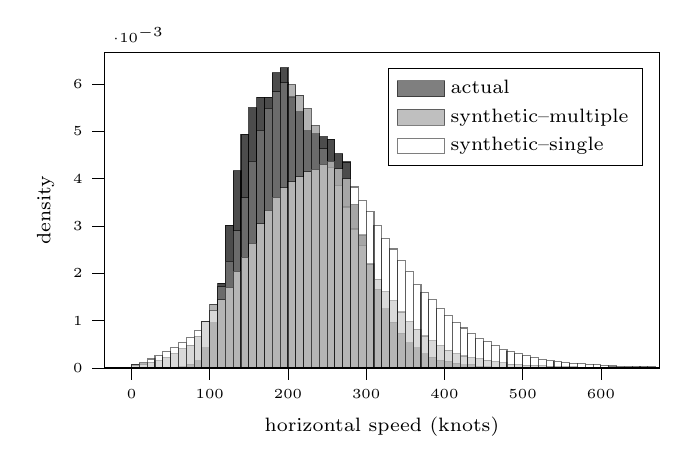
\begin{tikzpicture}

\begin{axis}[
legend cell align={left},
legend style={fill opacity=0.8, draw opacity=1, text opacity=1, draw=white!80!black},
width=3.4in,
height=2.2in,
tick align=outside,
tick pos=left,
x grid style={white!69.0196078431373!black},
xlabel={horizontal speed (knots)},
xmin=-35, xmax=675,
xtick style={color=black},
y grid style={white!69.0196078431373!black},
ytick={0.0, 0.001, 0.002, 0.003, 0.004, 0.005, 0.006},
ylabel={density},
ymin=0, ymax=0.00666249626531222,
ytick style={color=black},
% yticklabel style={/pgf/number format/.cd,fixed,precision=3},
tick label style={font=\tiny},
label style={font=\scriptsize},
legend entries={{actual},{synthetic--multiple}, {synthetic--single}},
legend style={at={(0.97,0.95)}, anchor=north east, draw=black},
legend style={font=\scriptsize}
]

\addlegendimage{area legend, draw=black, fill=black, opacity=0.5}
\addlegendimage{area legend, draw=black, fill=white!50.1960784313725!black, opacity=0.5}
\addlegendimage{area legend, draw=black, fill=white, opacity=0.5}

\draw[draw=black,fill=black,opacity=0.7] (axis cs:0,0) rectangle (axis cs:10,0);
\draw[draw=black,fill=black,opacity=0.7] (axis cs:10,0) rectangle (axis cs:20,0);
\draw[draw=black,fill=black,opacity=0.7] (axis cs:20,0) rectangle (axis cs:30,0);
\draw[draw=black,fill=black,opacity=0.7] (axis cs:30,0) rectangle (axis cs:40,1.86734389005079e-06);
\draw[draw=black,fill=black,opacity=0.7] (axis cs:40,0) rectangle (axis cs:50,3.73468778010158e-06);
\draw[draw=black,fill=black,opacity=0.7] (axis cs:50,0) rectangle (axis cs:60,3.73468778010158e-06);
\draw[draw=black,fill=black,opacity=0.7] (axis cs:60,0) rectangle (axis cs:70,2.98775022408127e-05);
\draw[draw=black,fill=black,opacity=0.7] (axis cs:70,0) rectangle (axis cs:80,7.65610994920825e-05);
\draw[draw=black,fill=black,opacity=0.7] (axis cs:80,0) rectangle (axis cs:90,0.000153122198984165);
\draw[draw=black,fill=black,opacity=0.7] (axis cs:90,0) rectangle (axis cs:100,0.00042388706304153);
\draw[draw=black,fill=black,opacity=0.7] (axis cs:100,0) rectangle (axis cs:110,0.000956080071706005);
\draw[draw=black,fill=black,opacity=0.7] (axis cs:110,0) rectangle (axis cs:120,0.00178891544666866);
\draw[draw=black,fill=black,opacity=0.7] (axis cs:120,0) rectangle (axis cs:130,0.00301202569465193);
\draw[draw=black,fill=black,opacity=0.7] (axis cs:130,0) rectangle (axis cs:140,0.00416417687481327);
\draw[draw=black,fill=black,opacity=0.7] (axis cs:140,0) rectangle (axis cs:150,0.00493912458918434);
\draw[draw=black,fill=black,opacity=0.7] (axis cs:150,0) rectangle (axis cs:160,0.00549932775619958);
\draw[draw=black,fill=black,opacity=0.7] (axis cs:160,0) rectangle (axis cs:170,0.00571780699133552);
\draw[draw=black,fill=black,opacity=0.7] (axis cs:170,0) rectangle (axis cs:180,0.00571593964744547);
\draw[draw=black,fill=black,opacity=0.7] (axis cs:180,0) rectangle (axis cs:190,0.00623506124887959);
\draw[draw=black,fill=black,opacity=0.7] (axis cs:190,0) rectangle (axis cs:200,0.00634523453839259);
\draw[draw=black,fill=black,opacity=0.7] (axis cs:200,0) rectangle (axis cs:210,0.00572154167911563);
\draw[draw=black,fill=black,opacity=0.7] (axis cs:210,0) rectangle (axis cs:220,0.0054152972811473);
\draw[draw=black,fill=black,opacity=0.7] (axis cs:220,0) rectangle (axis cs:230,0.00501008365700627);
\draw[draw=black,fill=black,opacity=0.7] (axis cs:230,0) rectangle (axis cs:240,0.0049447266208545);
\draw[draw=black,fill=black,opacity=0.7] (axis cs:240,0) rectangle (axis cs:250,0.00488123692859277);
\draw[draw=black,fill=black,opacity=0.7] (axis cs:250,0) rectangle (axis cs:260,0.00483268598745145);
\draw[draw=black,fill=black,opacity=0.7] (axis cs:260,0) rectangle (axis cs:270,0.00452830893337317);
\draw[draw=black,fill=black,opacity=0.7] (axis cs:270,0) rectangle (axis cs:280,0.00434904391992829);
\draw[draw=black,fill=black,opacity=0.7] (axis cs:280,0) rectangle (axis cs:290,0.00345832088437407);
\draw[draw=black,fill=black,opacity=0.7] (axis cs:290,0) rectangle (axis cs:300,0.00280848521063639);
\draw[draw=black,fill=black,opacity=0.7] (axis cs:300,0) rectangle (axis cs:310,0.00220533313414998);
\draw[draw=black,fill=black,opacity=0.7] (axis cs:310,0) rectangle (axis cs:320,0.00166380340603526);
\draw[draw=black,fill=black,opacity=0.7] (axis cs:320,0) rectangle (axis cs:330,0.00124925306244398);
\draw[draw=black,fill=black,opacity=0.7] (axis cs:330,0) rectangle (axis cs:340,0.00096728413504631);
\draw[draw=black,fill=black,opacity=0.7] (axis cs:340,0) rectangle (axis cs:350,0.000733866148789961);
\draw[draw=black,fill=black,opacity=0.7] (axis cs:350,0) rectangle (axis cs:360,0.000535927696444577);
\draw[draw=black,fill=black,opacity=0.7] (axis cs:360,0) rectangle (axis cs:370,0.000427621750821631);
\draw[draw=black,fill=black,opacity=0.7] (axis cs:370,0) rectangle (axis cs:380,0.000298775022408127);
\draw[draw=black,fill=black,opacity=0.7] (axis cs:380,0) rectangle (axis cs:390,0.000222213922916044);
\draw[draw=black,fill=black,opacity=0.7] (axis cs:390,0) rectangle (axis cs:400,0.000162458918434419);
\draw[draw=black,fill=black,opacity=0.7] (axis cs:400,0) rectangle (axis cs:410,0.000143785479533911);
\draw[draw=black,fill=black,opacity=0.7] (axis cs:410,0) rectangle (axis cs:420,0.000100836570062743);
\draw[draw=black,fill=black,opacity=0.7] (axis cs:420,0) rectangle (axis cs:430,7.09590678219301e-05);
\draw[draw=black,fill=black,opacity=0.7] (axis cs:430,0) rectangle (axis cs:440,7.46937556020317e-05);
\draw[draw=black,fill=black,opacity=0.7] (axis cs:440,0) rectangle (axis cs:450,3.73468778010158e-05);
\draw[draw=black,fill=black,opacity=0.7] (axis cs:450,0) rectangle (axis cs:460,2.61428144607111e-05);
\draw[draw=black,fill=black,opacity=0.7] (axis cs:460,0) rectangle (axis cs:470,1.68060950104571e-05);
\draw[draw=black,fill=black,opacity=0.7] (axis cs:470,0) rectangle (axis cs:480,1.86734389005079e-05);
\draw[draw=black,fill=black,opacity=0.7] (axis cs:480,0) rectangle (axis cs:490,1.12040633403048e-05);
\draw[draw=black,fill=black,opacity=0.7] (axis cs:490,0) rectangle (axis cs:500,5.60203167015238e-06);
\draw[draw=black,fill=black,opacity=0.7] (axis cs:500,0) rectangle (axis cs:510,3.73468778010158e-06);
\draw[draw=black,fill=black,opacity=0.7] (axis cs:510,0) rectangle (axis cs:520,1.86734389005079e-06);
\draw[draw=black,fill=black,opacity=0.7] (axis cs:520,0) rectangle (axis cs:530,1.86734389005079e-06);
\draw[draw=black,fill=black,opacity=0.7] (axis cs:530,0) rectangle (axis cs:540,1.86734389005079e-06);
\draw[draw=black,fill=black,opacity=0.7] (axis cs:540,0) rectangle (axis cs:550,0);
\draw[draw=black,fill=black,opacity=0.7] (axis cs:550,0) rectangle (axis cs:560,1.86734389005079e-06);
\draw[draw=black,fill=black,opacity=0.7] (axis cs:560,0) rectangle (axis cs:570,0);
\draw[draw=black,fill=black,opacity=0.7] (axis cs:570,0) rectangle (axis cs:580,0);
\draw[draw=black,fill=black,opacity=0.7] (axis cs:580,0) rectangle (axis cs:590,0);
\draw[draw=black,fill=black,opacity=0.7] (axis cs:590,0) rectangle (axis cs:600,0);
\draw[draw=black,fill=black,opacity=0.7] (axis cs:600,0) rectangle (axis cs:610,0);
\draw[draw=black,fill=black,opacity=0.7] (axis cs:610,0) rectangle (axis cs:620,0);
\draw[draw=black,fill=black,opacity=0.7] (axis cs:620,0) rectangle (axis cs:630,0);
\draw[draw=black,fill=black,opacity=0.7] (axis cs:630,0) rectangle (axis cs:640,0);
\draw[draw=black,fill=black,opacity=0.7] (axis cs:640,0) rectangle (axis cs:650,0);
\draw[draw=black,fill=black,opacity=0.7] (axis cs:650,0) rectangle (axis cs:660,0);
\draw[draw=black,fill=black,opacity=0.7] (axis cs:660,0) rectangle (axis cs:670,0);
\draw[draw=black,fill=black,opacity=0.7] (axis cs:670,0) rectangle (axis cs:680,0);
\draw[draw=black,fill=black,opacity=0.7] (axis cs:680,0) rectangle (axis cs:690,0);
\draw[draw=black,fill=black,opacity=0.7] (axis cs:690,0) rectangle (axis cs:700,0);
\draw[draw=black,fill=white!50.1960784313725!black,opacity=0.6] (axis cs:0,0) rectangle (axis cs:10,6.23251481972976e-05);
\draw[draw=black,fill=white!50.1960784313725!black,opacity=0.6] (axis cs:10,0) rectangle (axis cs:20,8.36837663997423e-05);
\draw[draw=black,fill=white!50.1960784313725!black,opacity=0.6] (axis cs:20,0) rectangle (axis cs:30,0.000123849973464293);
\draw[draw=black,fill=white!50.1960784313725!black,opacity=0.6] (axis cs:30,0) rectangle (axis cs:40,0.000149510327417113);
\draw[draw=black,fill=white!50.1960784313725!black,opacity=0.6] (axis cs:40,0) rectangle (axis cs:50,0.000220488967298305);
\draw[draw=black,fill=white!50.1960784313725!black,opacity=0.6] (axis cs:50,0) rectangle (axis cs:60,0.000300671320877974);
\draw[draw=black,fill=white!50.1960784313725!black,opacity=0.6] (axis cs:60,0) rectangle (axis cs:70,0.000402162272476944);
\draw[draw=black,fill=white!50.1960784313725!black,opacity=0.6] (axis cs:70,0) rectangle (axis cs:80,0.000480693960012865);
\draw[draw=black,fill=white!50.1960784313725!black,opacity=0.6] (axis cs:80,0) rectangle (axis cs:90,0.000672271261453997);
\draw[draw=black,fill=white!50.1960784313725!black,opacity=0.6] (axis cs:90,0) rectangle (axis cs:100,0.000973592844712842);
\draw[draw=black,fill=white!50.1960784313725!black,opacity=0.6] (axis cs:100,0) rectangle (axis cs:110,0.00134119117063735);
\draw[draw=black,fill=white!50.1960784313725!black,opacity=0.6] (axis cs:110,0) rectangle (axis cs:120,0.00171564226165258);
\draw[draw=black,fill=white!50.1960784313725!black,opacity=0.6] (axis cs:120,0) rectangle (axis cs:130,0.00224935761579797);
\draw[draw=black,fill=white!50.1960784313725!black,opacity=0.6] (axis cs:130,0) rectangle (axis cs:140,0.00289631866458116);
\draw[draw=black,fill=white!50.1960784313725!black,opacity=0.6] (axis cs:140,0) rectangle (axis cs:150,0.00359620106713059);
\draw[draw=black,fill=white!50.1960784313725!black,opacity=0.6] (axis cs:150,0) rectangle (axis cs:160,0.00436786243249151);
\draw[draw=black,fill=white!50.1960784313725!black,opacity=0.6] (axis cs:160,0) rectangle (axis cs:170,0.00501942533812393);
\draw[draw=black,fill=white!50.1960784313725!black,opacity=0.6] (axis cs:170,0) rectangle (axis cs:180,0.00548851461564741);
\draw[draw=black,fill=white!50.1960784313725!black,opacity=0.6] (axis cs:180,0) rectangle (axis cs:190,0.00583365387934031);
\draw[draw=black,fill=white!50.1960784313725!black,opacity=0.6] (axis cs:190,0) rectangle (axis cs:200,0.00602488103949944);
\draw[draw=black,fill=white!50.1960784313725!black,opacity=0.6] (axis cs:200,0) rectangle (axis cs:210,0.00597821220862618);
\draw[draw=black,fill=white!50.1960784313725!black,opacity=0.6] (axis cs:210,0) rectangle (axis cs:220,0.00575912380645591);
\draw[draw=black,fill=white!50.1960784313725!black,opacity=0.6] (axis cs:220,0) rectangle (axis cs:230,0.00547896076066693);
\draw[draw=black,fill=white!50.1960784313725!black,opacity=0.6] (axis cs:230,0) rectangle (axis cs:240,0.00511481382737935);
\draw[draw=black,fill=white!50.1960784313725!black,opacity=0.6] (axis cs:240,0) rectangle (axis cs:250,0.00463096859582842);
\draw[draw=black,fill=white!50.1960784313725!black,opacity=0.6] (axis cs:250,0) rectangle (axis cs:260,0.00423390838203215);
\draw[draw=black,fill=white!50.1960784313725!black,opacity=0.6] (axis cs:260,0) rectangle (axis cs:270,0.00385620597911257);
\draw[draw=black,fill=white!50.1960784313725!black,opacity=0.6] (axis cs:270,0) rectangle (axis cs:280,0.00340027200975594);
\draw[draw=black,fill=white!50.1960784313725!black,opacity=0.6] (axis cs:280,0) rectangle (axis cs:290,0.00293583460926484);
\draw[draw=black,fill=white!50.1960784313725!black,opacity=0.6] (axis cs:290,0) rectangle (axis cs:300,0.00258774415476645);
\draw[draw=black,fill=white!50.1960784313725!black,opacity=0.6] (axis cs:300,0) rectangle (axis cs:310,0.00217637816859103);
\draw[draw=black,fill=white!50.1960784313725!black,opacity=0.6] (axis cs:310,0) rectangle (axis cs:320,0.00187030466793351);
\draw[draw=black,fill=white!50.1960784313725!black,opacity=0.6] (axis cs:320,0) rectangle (axis cs:330,0.00161240060364357);
\draw[draw=black,fill=white!50.1960784313725!black,opacity=0.6] (axis cs:330,0) rectangle (axis cs:340,0.00142472487648766);
\draw[draw=black,fill=white!50.1960784313725!black,opacity=0.6] (axis cs:340,0) rectangle (axis cs:350,0.00118102654421059);
\draw[draw=black,fill=white!50.1960784313725!black,opacity=0.6] (axis cs:350,0) rectangle (axis cs:360,0.000977344358448634);
\draw[draw=black,fill=white!50.1960784313725!black,opacity=0.6] (axis cs:360,0) rectangle (axis cs:370,0.000817079691655583);
\draw[draw=black,fill=white!50.1960784313725!black,opacity=0.6] (axis cs:370,0) rectangle (axis cs:380,0.000674672230244904);
\draw[draw=black,fill=white!50.1960784313725!black,opacity=0.6] (axis cs:380,0) rectangle (axis cs:390,0.000577783135495172);
\draw[draw=black,fill=white!50.1960784313725!black,opacity=0.6] (axis cs:390,0) rectangle (axis cs:400,0.00047434139675359);
\draw[draw=black,fill=white!50.1960784313725!black,opacity=0.6] (axis cs:400,0) rectangle (axis cs:410,0.0003767019992567);
\draw[draw=black,fill=white!50.1960784313725!black,opacity=0.6] (axis cs:410,0) rectangle (axis cs:420,0.000303072289668881);
\draw[draw=black,fill=white!50.1960784313725!black,opacity=0.6] (axis cs:420,0) rectangle (axis cs:430,0.000253152146891271);
\draw[draw=black,fill=white!50.1960784313725!black,opacity=0.6] (axis cs:430,0) rectangle (axis cs:440,0.000219538583818571);
\draw[draw=black,fill=white!50.1960784313725!black,opacity=0.6] (axis cs:440,0) rectangle (axis cs:450,0.000192277584005146);
\draw[draw=black,fill=white!50.1960784313725!black,opacity=0.6] (axis cs:450,0) rectangle (axis cs:460,0.000160564787891914);
\draw[draw=black,fill=white!50.1960784313725!black,opacity=0.6] (axis cs:460,0) rectangle (axis cs:470,0.000128902011961827);
\draw[draw=black,fill=white!50.1960784313725!black,opacity=0.6] (axis cs:470,0) rectangle (axis cs:480,0.000110494584564872);
\draw[draw=black,fill=white!50.1960784313725!black,opacity=0.6] (axis cs:480,0) rectangle (axis cs:490,8.01823535796694e-05);
\draw[draw=black,fill=white!50.1960784313725!black,opacity=0.6] (axis cs:490,0) rectangle (axis cs:500,6.94280142037312e-05);
\draw[draw=black,fill=white!50.1960784313725!black,opacity=0.6] (axis cs:500,0) rectangle (axis cs:510,5.71730693334761e-05);
\draw[draw=black,fill=white!50.1960784313725!black,opacity=0.6] (axis cs:510,0) rectangle (axis cs:520,5.46720601762811e-05);
\draw[draw=black,fill=white!50.1960784313725!black,opacity=0.6] (axis cs:520,0) rectangle (axis cs:530,4.39677409834868e-05);
\draw[draw=black,fill=white!50.1960784313725!black,opacity=0.6] (axis cs:530,0) rectangle (axis cs:540,3.93158639511043e-05);
\draw[draw=black,fill=white!50.1960784313725!black,opacity=0.6] (axis cs:540,0) rectangle (axis cs:550,3.04122713514903e-05);
\draw[draw=black,fill=white!50.1960784313725!black,opacity=0.6] (axis cs:550,0) rectangle (axis cs:560,2.31093246124811e-05);
\draw[draw=black,fill=white!50.1960784313725!black,opacity=0.6] (axis cs:560,0) rectangle (axis cs:570,2.10084769204374e-05);
\draw[draw=black,fill=white!50.1960784313725!black,opacity=0.6] (axis cs:570,0) rectangle (axis cs:580,1.42057320128672e-05);
\draw[draw=black,fill=white!50.1960784313725!black,opacity=0.6] (axis cs:580,0) rectangle (axis cs:590,1.11044806579455e-05);
\draw[draw=black,fill=white!50.1960784313725!black,opacity=0.6] (axis cs:590,0) rectangle (axis cs:600,9.15369351533344e-06);
\draw[draw=black,fill=white!50.1960784313725!black,opacity=0.6] (axis cs:600,0) rectangle (axis cs:610,7.70310820416038e-06);
\draw[draw=black,fill=white!50.1960784313725!black,opacity=0.6] (axis cs:610,0) rectangle (axis cs:620,5.25211923010935e-06);
\draw[draw=black,fill=white!50.1960784313725!black,opacity=0.6] (axis cs:620,0) rectangle (axis cs:630,4.80193758181426e-06);
\draw[draw=black,fill=white!50.1960784313725!black,opacity=0.6] (axis cs:630,0) rectangle (axis cs:640,3.95159446836799e-06);
\draw[draw=black,fill=white!50.1960784313725!black,opacity=0.6] (axis cs:640,0) rectangle (axis cs:650,3.25131190435341e-06);
\draw[draw=black,fill=white!50.1960784313725!black,opacity=0.6] (axis cs:650,0) rectangle (axis cs:660,3.4013724537851e-06);
\draw[draw=black,fill=white!50.1960784313725!black,opacity=0.6] (axis cs:660,0) rectangle (axis cs:670,2.90117062234612e-06);
\draw[draw=black,fill=white!50.1960784313725!black,opacity=0.6] (axis cs:670,0) rectangle (axis cs:680,2.45098897405103e-06);
\draw[draw=black,fill=white!50.1960784313725!black,opacity=0.6] (axis cs:680,0) rectangle (axis cs:690,1.70068622689255e-06);
\draw[draw=black,fill=white!50.1960784313725!black,opacity=0.6] (axis cs:690,0) rectangle (axis cs:700,1.75070641003645e-06);
\draw[draw=black,fill=white,opacity=0.5] (axis cs:0,0) rectangle (axis cs:10,7.18621237649225e-05);
\draw[draw=black,fill=white,opacity=0.5] (axis cs:10,0) rectangle (axis cs:20,0.000115530884956449);
\draw[draw=black,fill=white,opacity=0.5] (axis cs:20,0) rectangle (axis cs:30,0.000189531427439514);
\draw[draw=black,fill=white,opacity=0.5] (axis cs:30,0) rectangle (axis cs:40,0.000254696924166045);
\draw[draw=black,fill=white,opacity=0.5] (axis cs:40,0) rectangle (axis cs:50,0.000339051915179059);
\draw[draw=black,fill=white,opacity=0.5] (axis cs:50,0) rectangle (axis cs:60,0.000427008453506838);
\draw[draw=black,fill=white,opacity=0.5] (axis cs:60,0) rectangle (axis cs:70,0.000532184889933338);
\draw[draw=black,fill=white,opacity=0.5] (axis cs:70,0) rectangle (axis cs:80,0.00063916210001722);
\draw[draw=black,fill=white,opacity=0.5] (axis cs:80,0) rectangle (axis cs:90,0.000793184521900221);
\draw[draw=black,fill=white,opacity=0.5] (axis cs:90,0) rectangle (axis cs:100,0.000972530323340165);
\draw[draw=black,fill=white,opacity=0.5] (axis cs:100,0) rectangle (axis cs:110,0.00121540967037964);
\draw[draw=black,fill=white,opacity=0.5] (axis cs:110,0) rectangle (axis cs:120,0.00144061892590604);
\draw[draw=black,fill=white,opacity=0.5] (axis cs:120,0) rectangle (axis cs:130,0.00170150600951934);
\draw[draw=black,fill=white,opacity=0.5] (axis cs:130,0) rectangle (axis cs:140,0.00204624161655451);
\draw[draw=black,fill=white,opacity=0.5] (axis cs:140,0) rectangle (axis cs:150,0.00233577225615555);
\draw[draw=black,fill=white,opacity=0.5] (axis cs:150,0) rectangle (axis cs:160,0.00263380029645236);
\draw[draw=black,fill=white,opacity=0.5] (axis cs:160,0) rectangle (axis cs:170,0.00304690902829128);
\draw[draw=black,fill=white,opacity=0.5] (axis cs:170,0) rectangle (axis cs:180,0.00332676050948389);
\draw[draw=black,fill=white,opacity=0.5] (axis cs:180,0) rectangle (axis cs:190,0.00360762492585877);
\draw[draw=black,fill=white,opacity=0.5] (axis cs:190,0) rectangle (axis cs:200,0.00380210848085609);
\draw[draw=black,fill=white,opacity=0.5] (axis cs:200,0) rectangle (axis cs:210,0.00393052615229818);
\draw[draw=black,fill=white,opacity=0.5] (axis cs:210,0) rectangle (axis cs:220,0.00404138628058079);
\draw[draw=black,fill=white,opacity=0.5] (axis cs:220,0) rectangle (axis cs:230,0.00414442429828915);
\draw[draw=black,fill=white,opacity=0.5] (axis cs:230,0) rectangle (axis cs:240,0.00419338283209924);
\draw[draw=black,fill=white,opacity=0.5] (axis cs:240,0) rectangle (axis cs:250,0.00430176689660295);
\draw[draw=black,fill=white,opacity=0.5] (axis cs:250,0) rectangle (axis cs:260,0.00436226163665565);
\draw[draw=black,fill=white,opacity=0.5] (axis cs:260,0) rectangle (axis cs:270,0.00420953352083889);
\draw[draw=black,fill=white,opacity=0.5] (axis cs:270,0) rectangle (axis cs:280,0.00399614184243906);
\draw[draw=black,fill=white,opacity=0.5] (axis cs:280,0) rectangle (axis cs:290,0.00382152307184974);
\draw[draw=black,fill=white,opacity=0.5] (axis cs:290,0) rectangle (axis cs:300,0.00354392255772886);
\draw[draw=black,fill=white,opacity=0.5] (axis cs:300,0) rectangle (axis cs:310,0.00329732911502104);
\draw[draw=black,fill=white,opacity=0.5] (axis cs:310,0) rectangle (axis cs:320,0.00300475966987317);
\draw[draw=black,fill=white,opacity=0.5] (axis cs:320,0) rectangle (axis cs:330,0.00273166108989575);
\draw[draw=black,fill=white,opacity=0.5] (axis cs:330,0) rectangle (axis cs:340,0.00251236062293263);
\draw[draw=black,fill=white,opacity=0.5] (axis cs:340,0) rectangle (axis cs:350,0.00226818696982691);
\draw[draw=black,fill=white,opacity=0.5] (axis cs:350,0) rectangle (axis cs:360,0.0020455100522562);
\draw[draw=black,fill=white,opacity=0.5] (axis cs:360,0) rectangle (axis cs:370,0.00177021677938384);
\draw[draw=black,fill=white,opacity=0.5] (axis cs:370,0) rectangle (axis cs:380,0.00158479336685023);
\draw[draw=black,fill=white,opacity=0.5] (axis cs:380,0) rectangle (axis cs:390,0.00144754064965161);
\draw[draw=black,fill=white,opacity=0.5] (axis cs:390,0) rectangle (axis cs:400,0.0012596411733391);
\draw[draw=black,fill=white,opacity=0.5] (axis cs:400,0) rectangle (axis cs:410,0.00109982251124639);
\draw[draw=black,fill=white,opacity=0.5] (axis cs:410,0) rectangle (axis cs:420,0.000958349230788277);
\draw[draw=black,fill=white,opacity=0.5] (axis cs:420,0) rectangle (axis cs:430,0.000842987168362208);
\draw[draw=black,fill=white,opacity=0.5] (axis cs:430,0) rectangle (axis cs:440,0.000718452415118846);
\draw[draw=black,fill=white,opacity=0.5] (axis cs:440,0) rectangle (axis cs:450,0.000624812184934953);
\draw[draw=black,fill=white,opacity=0.5] (axis cs:450,0) rectangle (axis cs:460,0.000550080078153577);
\draw[draw=black,fill=white,opacity=0.5] (axis cs:460,0) rectangle (axis cs:470,0.000472984455946886);
\draw[draw=black,fill=white,opacity=0.5] (axis cs:470,0) rectangle (axis cs:480,0.000394875898557918);
\draw[draw=black,fill=white,opacity=0.5] (axis cs:480,0) rectangle (axis cs:490,0.000343947768560068);
\draw[draw=black,fill=white,opacity=0.5] (axis cs:490,0) rectangle (axis cs:500,0.000308157392119589);
\draw[draw=black,fill=white,opacity=0.5] (axis cs:500,0) rectangle (axis cs:510,0.000257848278066464);
\draw[draw=black,fill=white,opacity=0.5] (axis cs:510,0) rectangle (axis cs:520,0.000220819869736536);
\draw[draw=black,fill=white,opacity=0.5] (axis cs:520,0) rectangle (axis cs:530,0.000182891074577916);
\draw[draw=black,fill=white,opacity=0.5] (axis cs:530,0) rectangle (axis cs:540,0.000161619435750084);
\draw[draw=black,fill=white,opacity=0.5] (axis cs:540,0) rectangle (axis cs:550,0.000145581295364021);
\draw[draw=black,fill=white,opacity=0.5] (axis cs:550,0) rectangle (axis cs:560,0.000120370464160665);
\draw[draw=black,fill=white,opacity=0.5] (axis cs:560,0) rectangle (axis cs:570,0.000101124695697389);
\draw[draw=black,fill=white,opacity=0.5] (axis cs:570,0) rectangle (axis cs:580,9.13892631121646e-05);
\draw[draw=black,fill=white,opacity=0.5] (axis cs:580,0) rectangle (axis cs:590,8.08659920518353e-05);
\draw[draw=black,fill=white,opacity=0.5] (axis cs:590,0) rectangle (axis cs:600,6.98925275771603e-05);
\draw[draw=black,fill=white,opacity=0.5] (axis cs:600,0) rectangle (axis cs:610,5.64429993235844e-05);
\draw[draw=black,fill=white,opacity=0.5] (axis cs:610,0) rectangle (axis cs:620,4.19805358877308e-05);
\draw[draw=black,fill=white,opacity=0.5] (axis cs:620,0) rectangle (axis cs:630,3.72535050371016e-05);
\draw[draw=black,fill=white,opacity=0.5] (axis cs:630,0) rectangle (axis cs:640,3.33143126615772e-05);
\draw[draw=black,fill=white,opacity=0.5] (axis cs:640,0) rectangle (axis cs:650,3.0781974705883e-05);
\draw[draw=black,fill=white,opacity=0.5] (axis cs:650,0) rectangle (axis cs:660,2.82496367501888e-05);
\draw[draw=black,fill=white,opacity=0.5] (axis cs:660,0) rectangle (axis cs:670,2.13841871814178e-05);
\draw[draw=black,fill=white,opacity=0.5] (axis cs:670,0) rectangle (axis cs:680,1.82328332809983e-05);
\draw[draw=black,fill=white,opacity=0.5] (axis cs:680,0) rectangle (axis cs:690,1.457501178944e-05);
\draw[draw=black,fill=white,opacity=0.5] (axis cs:690,0) rectangle (axis cs:700,1.25491414248847e-05);
\end{axis}

\end{tikzpicture}
}
    \hspace*{1em}%
    \subfigure[distance to the closest aircraft. $D_{JS}$: 0.0307 (multiple), 0.0261 (single)]{
        \label{fig:hist_encounter}
        % This file was created by tikzplotlib v0.9.2.
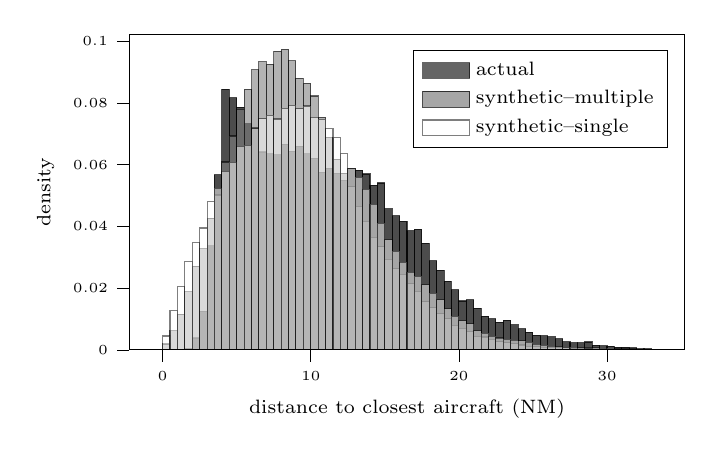
\begin{tikzpicture}

\begin{axis}[
legend cell align={left},
legend style={fill opacity=0.8, draw opacity=1, text opacity=1, draw=white!80!black},
width=3.4in,
height=2.2in,
tick align=outside,
tick pos=left,
x grid style={white!69.0196078431373!black},
xlabel={distance to closest aircraft (NM)},
xmin=-2.25, xmax=35.25,
xtick style={color=black},
y grid style={white!69.0196078431373!black},
ylabel={density},
ytick={0, 0.02, 0.04, 0.06, 0.08, 0.10},
yticklabel style={/pgf/number format/.cd,fixed,precision=2},
ymin=0, ymax=0.102280215023725,
ytick style={color=black},
tick label style={font=\tiny},
label style={font=\scriptsize},
legend cell align={left},
legend entries={{actual},{synthetic--multiple}, {synthetic--single}},
legend style={at={(0.97,0.95)}, anchor=north east, draw=black},
legend style={font=\scriptsize}
]

\addlegendimage{area legend, draw=black, fill=black, opacity=0.6}
\addlegendimage{area legend, draw=black, fill=white!50.1960784313725!black, opacity=0.7}
\addlegendimage{area legend, draw=black, fill=white, opacity=0.5}

\draw[draw=black,fill=black,opacity=0.7] (axis cs:0,0) rectangle (axis cs:0.5,1.65058265567745e-05);
\draw[draw=black,fill=black,opacity=0.7] (axis cs:0.5,0) rectangle (axis cs:1,9.90349593406472e-05);
\draw[draw=black,fill=black,opacity=0.7] (axis cs:1,0) rectangle (axis cs:1.5,0.000148552439010971);
\draw[draw=black,fill=black,opacity=0.7] (axis cs:1.5,0) rectangle (axis cs:2,0.00054469227637356);
\draw[draw=black,fill=black,opacity=0.7] (axis cs:2,0) rectangle (axis cs:2.5,0.00382935176117169);
\draw[draw=black,fill=black,opacity=0.7] (axis cs:2.5,0) rectangle (axis cs:3,0.0124949107034783);
\draw[draw=black,fill=black,opacity=0.7] (axis cs:3,0) rectangle (axis cs:3.5,0.0336828900601912);
\draw[draw=black,fill=black,opacity=0.7] (axis cs:3.5,0) rectangle (axis cs:4,0.0567305258756341);
\draw[draw=black,fill=black,opacity=0.7] (axis cs:4,0) rectangle (axis cs:4.5,0.0844438086644586);
\draw[draw=black,fill=black,opacity=0.7] (axis cs:4.5,0) rectangle (axis cs:5,0.0817368531091475);
\draw[draw=black,fill=black,opacity=0.7] (axis cs:5,0) rectangle (axis cs:5.5,0.0786832751961442);
\draw[draw=black,fill=black,opacity=0.7] (axis cs:5.5,0) rectangle (axis cs:6,0.0733628971026773);
\draw[draw=black,fill=black,opacity=0.7] (axis cs:6,0) rectangle (axis cs:6.5,0.0720699406890632);
\draw[draw=black,fill=black,opacity=0.7] (axis cs:6.5,0) rectangle (axis cs:7,0.0641361400574403);
\draw[draw=black,fill=black,opacity=0.7] (axis cs:7,0) rectangle (axis cs:7.5,0.0635254244748396);
\draw[draw=black,fill=black,opacity=0.7] (axis cs:7.5,0) rectangle (axis cs:8,0.0632338215390033);
\draw[draw=black,fill=black,opacity=0.7] (axis cs:8,0) rectangle (axis cs:8.5,0.0666120140409565);
\draw[draw=black,fill=black,opacity=0.7] (axis cs:8.5,0) rectangle (axis cs:9,0.064328708033936);
\draw[draw=black,fill=black,opacity=0.7] (axis cs:9,0) rectangle (axis cs:9.5,0.0659682868052422);
\draw[draw=black,fill=black,opacity=0.7] (axis cs:9.5,0) rectangle (axis cs:10,0.0635584361279532);
\draw[draw=black,fill=black,opacity=0.7] (axis cs:10,0) rectangle (axis cs:10.5,0.0620454020269155);
\draw[draw=black,fill=black,opacity=0.7] (axis cs:10.5,0) rectangle (axis cs:11,0.0575833269144008);
\draw[draw=black,fill=black,opacity=0.7] (axis cs:11,0) rectangle (axis cs:11.5,0.0588322677905301);
\draw[draw=black,fill=black,opacity=0.7] (axis cs:11.5,0) rectangle (axis cs:12,0.057176183192667);
\draw[draw=black,fill=black,opacity=0.7] (axis cs:12,0) rectangle (axis cs:12.5,0.0549148849543889);
\draw[draw=black,fill=black,opacity=0.7] (axis cs:12.5,0) rectangle (axis cs:13,0.0586617075827767);
\draw[draw=black,fill=black,opacity=0.7] (axis cs:13,0) rectangle (axis cs:13.5,0.0582655677454141);
\draw[draw=black,fill=black,opacity=0.7] (axis cs:13.5,0) rectangle (axis cs:14,0.0569781132739857);
\draw[draw=black,fill=black,opacity=0.7] (axis cs:14,0) rectangle (axis cs:14.5,0.05339084696898);
\draw[draw=black,fill=black,opacity=0.7] (axis cs:14.5,0) rectangle (axis cs:15,0.0540620839156222);
\draw[draw=black,fill=black,opacity=0.7] (axis cs:15,0) rectangle (axis cs:15.5,0.0457761589841214);
\draw[draw=black,fill=black,opacity=0.7] (axis cs:15.5,0) rectangle (axis cs:16,0.0434708452083586);
\draw[draw=black,fill=black,opacity=0.7] (axis cs:16,0) rectangle (axis cs:16.5,0.0416166906918142);
\draw[draw=black,fill=black,opacity=0.7] (axis cs:16.5,0) rectangle (axis cs:17,0.0385796186053677);
\draw[draw=black,fill=black,opacity=0.7] (axis cs:17,0) rectangle (axis cs:17.5,0.039047283691143);
\draw[draw=black,fill=black,opacity=0.7] (axis cs:17.5,0) rectangle (axis cs:18,0.0345852085786283);
\draw[draw=black,fill=black,opacity=0.7] (axis cs:18,0) rectangle (axis cs:18.5,0.0288191731681283);
\draw[draw=black,fill=black,opacity=0.7] (axis cs:18.5,0) rectangle (axis cs:19,0.0258481243879089);
\draw[draw=black,fill=black,opacity=0.7] (axis cs:19,0) rectangle (axis cs:19.5,0.022183830892305);
\draw[draw=black,fill=black,opacity=0.7] (axis cs:19.5,0) rectangle (axis cs:20,0.0194713733948084);
\draw[draw=black,fill=black,opacity=0.7] (axis cs:20,0) rectangle (axis cs:20.5,0.0158235857257612);
\draw[draw=black,fill=black,opacity=0.7] (axis cs:20.5,0) rectangle (axis cs:21,0.0161867139100102);
\draw[draw=black,fill=black,opacity=0.7] (axis cs:21,0) rectangle (axis cs:21.5,0.0133972292219153);
\draw[draw=black,fill=black,opacity=0.7] (axis cs:21.5,0) rectangle (axis cs:22,0.0108498299899865);
\draw[draw=black,fill=black,opacity=0.7] (axis cs:22,0) rectangle (axis cs:22.5,0.0100190367199621);
\draw[draw=black,fill=black,opacity=0.7] (axis cs:22.5,0) rectangle (axis cs:23,0.00895165993595739);
\draw[draw=black,fill=black,opacity=0.7] (axis cs:23,0) rectangle (axis cs:23.5,0.0095293638654445);
\draw[draw=black,fill=black,opacity=0.7] (axis cs:23.5,0) rectangle (axis cs:24,0.00819239191434576);
\draw[draw=black,fill=black,opacity=0.7] (axis cs:24,0) rectangle (axis cs:24.5,0.00676738888827756);
\draw[draw=black,fill=black,opacity=0.7] (axis cs:24.5,0) rectangle (axis cs:25,0.00561198102930334);
\draw[draw=black,fill=black,opacity=0.7] (axis cs:25,0) rectangle (axis cs:25.5,0.00464914114682483);
\draw[draw=black,fill=black,opacity=0.7] (axis cs:25.5,0) rectangle (axis cs:26,0.00452259647655622);
\draw[draw=black,fill=black,opacity=0.7] (axis cs:26,0) rectangle (axis cs:26.5,0.00418147606104955);
\draw[draw=black,fill=black,opacity=0.7] (axis cs:26.5,0) rectangle (axis cs:27,0.00363678378467599);
\draw[draw=black,fill=black,opacity=0.7] (axis cs:27,0) rectangle (axis cs:27.5,0.00264643419126952);
\draw[draw=black,fill=black,opacity=0.7] (axis cs:27.5,0) rectangle (axis cs:28,0.00232732154450521);
\draw[draw=black,fill=black,opacity=0.7] (axis cs:28,0) rectangle (axis cs:28.5,0.00223929046953575);
\draw[draw=black,fill=black,opacity=0.7] (axis cs:28.5,0) rectangle (axis cs:29,0.00251438757881532);
\draw[draw=black,fill=black,opacity=0.7] (axis cs:29,0) rectangle (axis cs:29.5,0.00151303410103767);
\draw[draw=black,fill=black,opacity=0.7] (axis cs:29.5,0) rectangle (axis cs:30,0.00124894087612927);
\draw[draw=black,fill=black,opacity=0.7] (axis cs:30,0) rectangle (axis cs:30.5,0.00113890203241744);
\draw[draw=black,fill=black,opacity=0.7] (axis cs:30.5,0) rectangle (axis cs:31,0.00083629521220991);
\draw[draw=black,fill=black,opacity=0.7] (axis cs:31,0) rectangle (axis cs:31.5,0.000792279674725178);
\draw[draw=black,fill=black,opacity=0.7] (axis cs:31.5,0) rectangle (axis cs:32,0.000698746657570122);
\draw[draw=black,fill=black,opacity=0.7] (axis cs:32,0) rectangle (axis cs:32.5,0.000269595167093984);
\draw[draw=black,fill=black,opacity=0.7] (axis cs:32.5,0) rectangle (axis cs:33,0.000242085456166027);
\draw[draw=black,fill=black,opacity=0.7] (axis cs:33,0) rectangle (axis cs:33.5,0.000214575745238069);
\draw[draw=black,fill=black,opacity=0.7] (axis cs:33.5,0) rectangle (axis cs:34,0.000198069918681294);
\draw[draw=black,fill=black,opacity=0.7] (axis cs:34,0) rectangle (axis cs:34.5,0.000148552439010971);
\draw[draw=black,fill=black,opacity=0.7] (axis cs:34.5,0) rectangle (axis cs:35,0.000137548554639788);
\draw[draw=black,fill=white!50.1960784313725!black,opacity=0.6] (axis cs:0,0) rectangle (axis cs:0.5,0.00186518945891941);
\draw[draw=black,fill=white!50.1960784313725!black,opacity=0.6] (axis cs:0.5,0) rectangle (axis cs:1,0.00625131211478192);
\draw[draw=black,fill=white!50.1960784313725!black,opacity=0.6] (axis cs:1,0) rectangle (axis cs:1.5,0.0114872251250221);
\draw[draw=black,fill=white!50.1960784313725!black,opacity=0.6] (axis cs:1.5,0) rectangle (axis cs:2,0.018770664500928);
\draw[draw=black,fill=white!50.1960784313725!black,opacity=0.6] (axis cs:2,0) rectangle (axis cs:2.5,0.0271247058980971);
\draw[draw=black,fill=white!50.1960784313725!black,opacity=0.6] (axis cs:2.5,0) rectangle (axis cs:3,0.032770458744602);
\draw[draw=black,fill=white!50.1960784313725!black,opacity=0.6] (axis cs:3,0) rectangle (axis cs:3.5,0.0426501080220711);
\draw[draw=black,fill=white!50.1960784313725!black,opacity=0.6] (axis cs:3.5,0) rectangle (axis cs:4,0.0501710872214448);
\draw[draw=black,fill=white!50.1960784313725!black,opacity=0.6] (axis cs:4,0) rectangle (axis cs:4.5,0.0608854715123675);
\draw[draw=black,fill=white!50.1960784313725!black,opacity=0.6] (axis cs:4.5,0) rectangle (axis cs:5,0.0693264993237643);
\draw[draw=black,fill=white!50.1960784313725!black,opacity=0.6] (axis cs:5,0) rectangle (axis cs:5.5,0.077976629092439);
\draw[draw=black,fill=white!50.1960784313725!black,opacity=0.6] (axis cs:5.5,0) rectangle (axis cs:6,0.0844002412200179);
\draw[draw=black,fill=white!50.1960784313725!black,opacity=0.6] (axis cs:6,0) rectangle (axis cs:6.5,0.0908539640294449);
\draw[draw=black,fill=white!50.1960784313725!black,opacity=0.6] (axis cs:6.5,0) rectangle (axis cs:7,0.0933314040192742);
\draw[draw=black,fill=white!50.1960784313725!black,opacity=0.6] (axis cs:7,0) rectangle (axis cs:7.5,0.0926304942584785);
\draw[draw=black,fill=white!50.1960784313725!black,opacity=0.6] (axis cs:7.5,0) rectangle (axis cs:8,0.0968493353485186);
\draw[draw=black,fill=white!50.1960784313725!black,opacity=0.6] (axis cs:8,0) rectangle (axis cs:8.5,0.0974097285940235);
\draw[draw=black,fill=white!50.1960784313725!black,opacity=0.6] (axis cs:8.5,0) rectangle (axis cs:9,0.0936709855978936);
\draw[draw=black,fill=white!50.1960784313725!black,opacity=0.6] (axis cs:9,0) rectangle (axis cs:9.5,0.0880770900367936);
\draw[draw=black,fill=white!50.1960784313725!black,opacity=0.6] (axis cs:9.5,0) rectangle (axis cs:10,0.0863741636967219);
\draw[draw=black,fill=white!50.1960784313725!black,opacity=0.6] (axis cs:10,0) rectangle (axis cs:10.5,0.0822924934906561);
\draw[draw=black,fill=white!50.1960784313725!black,opacity=0.6] (axis cs:10.5,0) rectangle (axis cs:11,0.0753252162741544);
\draw[draw=black,fill=white!50.1960784313725!black,opacity=0.6] (axis cs:11,0) rectangle (axis cs:11.5,0.0688781847273603);
\draw[draw=black,fill=white!50.1960784313725!black,opacity=0.6] (axis cs:11.5,0) rectangle (axis cs:12,0.0618289395436057);
\draw[draw=black,fill=white!50.1960784313725!black,opacity=0.6] (axis cs:12,0) rectangle (axis cs:12.5,0.0572638256123133);
\draw[draw=black,fill=white!50.1960784313725!black,opacity=0.6] (axis cs:12.5,0) rectangle (axis cs:13,0.0528040990674889);
\draw[draw=black,fill=white!50.1960784313725!black,opacity=0.6] (axis cs:13,0) rectangle (axis cs:13.5,0.0464959112203274);
\draw[draw=black,fill=white!50.1960784313725!black,opacity=0.6] (axis cs:13.5,0) rectangle (axis cs:14,0.0417250409630734);
\draw[draw=black,fill=white!50.1960784313725!black,opacity=0.6] (axis cs:14,0) rectangle (axis cs:14.5,0.0365192386346813);
\draw[draw=black,fill=white!50.1960784313725!black,opacity=0.6] (axis cs:14.5,0) rectangle (axis cs:15,0.0334546403488155);
\draw[draw=black,fill=white!50.1960784313725!black,opacity=0.6] (axis cs:15,0) rectangle (axis cs:15.5,0.0293913711149902);
\draw[draw=black,fill=white!50.1960784313725!black,opacity=0.6] (axis cs:15.5,0) rectangle (axis cs:16,0.0262799339906941);
\draw[draw=black,fill=white!50.1960784313725!black,opacity=0.6] (axis cs:16,0) rectangle (axis cs:16.5,0.0245335144435086);
\draw[draw=black,fill=white!50.1960784313725!black,opacity=0.6] (axis cs:16.5,0) rectangle (axis cs:17,0.021440478291453);
\draw[draw=black,fill=white!50.1960784313725!black,opacity=0.6] (axis cs:17,0) rectangle (axis cs:17.5,0.0189864577208388);
\draw[draw=black,fill=white!50.1960784313725!black,opacity=0.6] (axis cs:17.5,0) rectangle (axis cs:18,0.0155521671745056);
\draw[draw=black,fill=white!50.1960784313725!black,opacity=0.6] (axis cs:18,0) rectangle (axis cs:18.5,0.0135665349881941);
\draw[draw=black,fill=white!50.1960784313725!black,opacity=0.6] (axis cs:18.5,0) rectangle (axis cs:19,0.0116478154282115);
\draw[draw=black,fill=white!50.1960784313725!black,opacity=0.6] (axis cs:19,0) rectangle (axis cs:19.5,0.0101389357044938);
\draw[draw=black,fill=white!50.1960784313725!black,opacity=0.6] (axis cs:19.5,0) rectangle (axis cs:20,0.00801278700289146);
\draw[draw=black,fill=white!50.1960784313725!black,opacity=0.6] (axis cs:20,0) rectangle (axis cs:20.5,0.00697564129479278);
\draw[draw=black,fill=white!50.1960784313725!black,opacity=0.6] (axis cs:20.5,0) rectangle (axis cs:21,0.00582808975325133);
\draw[draw=black,fill=white!50.1960784313725!black,opacity=0.6] (axis cs:21,0) rectangle (axis cs:21.5,0.00439783236547007);
\draw[draw=black,fill=white!50.1960784313725!black,opacity=0.6] (axis cs:21.5,0) rectangle (axis cs:22,0.00413687312278718);
\draw[draw=black,fill=white!50.1960784313725!black,opacity=0.6] (axis cs:22,0) rectangle (axis cs:22.5,0.00347276530647237);
\draw[draw=black,fill=white!50.1960784313725!black,opacity=0.6] (axis cs:22.5,0) rectangle (axis cs:23,0.00263468466170231);
\draw[draw=black,fill=white!50.1960784313725!black,opacity=0.6] (axis cs:23,0) rectangle (axis cs:23.5,0.00227837492650066);
\draw[draw=black,fill=white!50.1960784313725!black,opacity=0.6] (axis cs:23.5,0) rectangle (axis cs:24,0.00197224966104573);
\draw[draw=black,fill=white!50.1960784313725!black,opacity=0.6] (axis cs:24,0) rectangle (axis cs:24.5,0.00154568166819869);
\draw[draw=black,fill=white!50.1960784313725!black,opacity=0.6] (axis cs:24.5,0) rectangle (axis cs:25,0.00117431659207303);
\draw[draw=black,fill=white!50.1960784313725!black,opacity=0.6] (axis cs:25,0) rectangle (axis cs:25.5,0.000936776768605265);
\draw[draw=black,fill=white!50.1960784313725!black,opacity=0.6] (axis cs:25.5,0) rectangle (axis cs:26,0.000841426276086515);
\draw[draw=black,fill=white!50.1960784313725!black,opacity=0.6] (axis cs:26,0) rectangle (axis cs:26.5,0.000685854419871712);
\draw[draw=black,fill=white!50.1960784313725!black,opacity=0.6] (axis cs:26.5,0) rectangle (axis cs:27,0.00063065150315033);
\draw[draw=black,fill=white!50.1960784313725!black,opacity=0.6] (axis cs:27,0) rectangle (axis cs:27.5,0.000628978687492106);
\draw[draw=black,fill=white!50.1960784313725!black,opacity=0.6] (axis cs:27.5,0) rectangle (axis cs:28,0.000396457310999014);
\draw[draw=black,fill=white!50.1960784313725!black,opacity=0.6] (axis cs:28,0) rectangle (axis cs:28.5,0.00037638352310033);
\draw[draw=black,fill=white!50.1960784313725!black,opacity=0.6] (axis cs:28.5,0) rectangle (axis cs:29,0.000368019444809211);
\draw[draw=black,fill=white!50.1960784313725!black,opacity=0.6] (axis cs:29,0) rectangle (axis cs:29.5,0.000292742740189145);
\draw[draw=black,fill=white!50.1960784313725!black,opacity=0.6] (axis cs:29.5,0) rectangle (axis cs:30,0.000225830113860198);
\draw[draw=black,fill=white!50.1960784313725!black,opacity=0.6] (axis cs:30,0) rectangle (axis cs:30.5,0.000210774772936185);
\draw[draw=black,fill=white!50.1960784313725!black,opacity=0.6] (axis cs:30.5,0) rectangle (axis cs:31,0.000192373800695724);
\draw[draw=black,fill=white!50.1960784313725!black,opacity=0.6] (axis cs:31,0) rectangle (axis cs:31.5,0.000127133990025);
\draw[draw=black,fill=white!50.1960784313725!black,opacity=0.6] (axis cs:31.5,0) rectangle (axis cs:32,0.000117097096075658);
\draw[draw=black,fill=white!50.1960784313725!black,opacity=0.6] (axis cs:32,0) rectangle (axis cs:32.5,0.000113751464759211);
\draw[draw=black,fill=white!50.1960784313725!black,opacity=0.6] (axis cs:32.5,0) rectangle (axis cs:33,9.86961238351975e-05);
\draw[draw=black,fill=white!50.1960784313725!black,opacity=0.6] (axis cs:33,0) rectangle (axis cs:33.5,8.69864142276317e-05);
\draw[draw=black,fill=white!50.1960784313725!black,opacity=0.6] (axis cs:33.5,0) rectangle (axis cs:34,7.69495202782896e-05);
\draw[draw=black,fill=white!50.1960784313725!black,opacity=0.6] (axis cs:34,0) rectangle (axis cs:34.5,8.36407829111844e-05);
\draw[draw=black,fill=white!50.1960784313725!black,opacity=0.6] (axis cs:34.5,0) rectangle (axis cs:35,7.86223359365133e-05);
\draw[draw=black,fill=white,opacity=0.5] (axis cs:0,0) rectangle (axis cs:0.5,0.00447782186497453);
\draw[draw=black,fill=white,opacity=0.5] (axis cs:0.5,0) rectangle (axis cs:1,0.0128077186932797);
\draw[draw=black,fill=white,opacity=0.5] (axis cs:1,0) rectangle (axis cs:1.5,0.020611375772496);
\draw[draw=black,fill=white,opacity=0.5] (axis cs:1.5,0) rectangle (axis cs:2,0.0285700343778076);
\draw[draw=black,fill=white,opacity=0.5] (axis cs:2,0) rectangle (axis cs:2.5,0.0348944793623122);
\draw[draw=black,fill=white,opacity=0.5] (axis cs:2.5,0) rectangle (axis cs:3,0.0394966851679805);
\draw[draw=black,fill=white,opacity=0.5] (axis cs:3,0) rectangle (axis cs:3.5,0.0482207834083305);
\draw[draw=black,fill=white,opacity=0.5] (axis cs:3.5,0) rectangle (axis cs:4,0.0523866886220269);
\draw[draw=black,fill=white,opacity=0.5] (axis cs:4,0) rectangle (axis cs:4.5,0.0579476075705807);
\draw[draw=black,fill=white,opacity=0.5] (axis cs:4.5,0) rectangle (axis cs:5,0.0608467101882886);
\draw[draw=black,fill=white,opacity=0.5] (axis cs:5,0) rectangle (axis cs:5.5,0.0659579333512574);
\draw[draw=black,fill=white,opacity=0.5] (axis cs:5.5,0) rectangle (axis cs:6,0.0663693571550905);
\draw[draw=black,fill=white,opacity=0.5] (axis cs:6,0) rectangle (axis cs:6.5,0.0716183594523662);
\draw[draw=black,fill=white,opacity=0.5] (axis cs:6.5,0) rectangle (axis cs:7,0.0749556762611336);
\draw[draw=black,fill=white,opacity=0.5] (axis cs:7,0) rectangle (axis cs:7.5,0.0760732181282896);
\draw[draw=black,fill=white,opacity=0.5] (axis cs:7.5,0) rectangle (axis cs:8,0.0748102427304763);
\draw[draw=black,fill=white,opacity=0.5] (axis cs:8,0) rectangle (axis cs:8.5,0.0782394122954482);
\draw[draw=black,fill=white,opacity=0.5] (axis cs:8.5,0) rectangle (axis cs:9,0.079282323798188);
\draw[draw=black,fill=white,opacity=0.5] (axis cs:9,0) rectangle (axis cs:9.5,0.0781839179219079);
\draw[draw=black,fill=white,opacity=0.5] (axis cs:9.5,0) rectangle (axis cs:10,0.0790507783085889);
\draw[draw=black,fill=white,opacity=0.5] (axis cs:10,0) rectangle (axis cs:10.5,0.0753441368759155);
\draw[draw=black,fill=white,opacity=0.5] (axis cs:10.5,0) rectangle (axis cs:11,0.0747757979468995);
\draw[draw=black,fill=white,opacity=0.5] (axis cs:11,0) rectangle (axis cs:11.5,0.0718097193611258);
\draw[draw=black,fill=white,opacity=0.5] (axis cs:11.5,0) rectangle (axis cs:12,0.0689278391352063);
\draw[draw=black,fill=white,opacity=0.5] (axis cs:12,0) rectangle (axis cs:12.5,0.0636597008470546);
\draw[draw=black,fill=white,opacity=0.5] (axis cs:12.5,0) rectangle (axis cs:13,0.0586958248138307);
\draw[draw=black,fill=white,opacity=0.5] (axis cs:13,0) rectangle (axis cs:13.5,0.0558713525605391);
\draw[draw=black,fill=white,opacity=0.5] (axis cs:13.5,0) rectangle (axis cs:14,0.0519714376200185);
\draw[draw=black,fill=white,opacity=0.5] (axis cs:14,0) rectangle (axis cs:14.5,0.0471281183293132);
\draw[draw=black,fill=white,opacity=0.5] (axis cs:14.5,0) rectangle (axis cs:15,0.0409567612718162);
\draw[draw=black,fill=white,opacity=0.5] (axis cs:15,0) rectangle (axis cs:15.5,0.0357364629608545);
\draw[draw=black,fill=white,opacity=0.5] (axis cs:15.5,0) rectangle (axis cs:16,0.0319800679519036);
\draw[draw=black,fill=white,opacity=0.5] (axis cs:16,0) rectangle (axis cs:16.5,0.0284437368380263);
\draw[draw=black,fill=white,opacity=0.5] (axis cs:16.5,0) rectangle (axis cs:17,0.0251351240155729);
\draw[draw=black,fill=white,opacity=0.5] (axis cs:17,0) rectangle (axis cs:17.5,0.0237688142670294);
\draw[draw=black,fill=white,opacity=0.5] (axis cs:17.5,0) rectangle (axis cs:18,0.0211050843370958);
\draw[draw=black,fill=white,opacity=0.5] (axis cs:18,0) rectangle (axis cs:18.5,0.0183341928582568);
\draw[draw=black,fill=white,opacity=0.5] (axis cs:18.5,0) rectangle (axis cs:19,0.0161718258892734);
\draw[draw=black,fill=white,opacity=0.5] (axis cs:19,0) rectangle (axis cs:19.5,0.0133530944332446);
\draw[draw=black,fill=white,opacity=0.5] (axis cs:19.5,0) rectangle (axis cs:20,0.0109189963938225);
\draw[draw=black,fill=white,opacity=0.5] (axis cs:20,0) rectangle (axis cs:20.5,0.00935749953834422);
\draw[draw=black,fill=white,opacity=0.5] (axis cs:20.5,0) rectangle (axis cs:21,0.0084676759626121);
\draw[draw=black,fill=white,opacity=0.5] (axis cs:21,0) rectangle (axis cs:21.5,0.00620006104381089);
\draw[draw=black,fill=white,opacity=0.5] (axis cs:21.5,0) rectangle (axis cs:22,0.00530449667081599);
\draw[draw=black,fill=white,opacity=0.5] (axis cs:22,0) rectangle (axis cs:22.5,0.0043534379242808);
\draw[draw=black,fill=white,opacity=0.5] (axis cs:22.5,0) rectangle (axis cs:23,0.00381188938249114);
\draw[draw=black,fill=white,opacity=0.5] (axis cs:23,0) rectangle (axis cs:23.5,0.00336793439416888);
\draw[draw=black,fill=white,opacity=0.5] (axis cs:23.5,0) rectangle (axis cs:24,0.00315169769727054);
\draw[draw=black,fill=white,opacity=0.5] (axis cs:24,0) rectangle (axis cs:24.5,0.00287805302774432);
\draw[draw=black,fill=white,opacity=0.5] (axis cs:24.5,0) rectangle (axis cs:25,0.00240539405310812);
\draw[draw=black,fill=white,opacity=0.5] (axis cs:25,0) rectangle (axis cs:25.5,0.00178538794872703);
\draw[draw=black,fill=white,opacity=0.5] (axis cs:25.5,0) rectangle (axis cs:26,0.00147347129744889);
\draw[draw=black,fill=white,opacity=0.5] (axis cs:26,0) rectangle (axis cs:26.5,0.00116920904252113);
\draw[draw=black,fill=white,opacity=0.5] (axis cs:26.5,0) rectangle (axis cs:27,0.00102951630912662);
\draw[draw=black,fill=white,opacity=0.5] (axis cs:27,0) rectangle (axis cs:27.5,0.000876428382118947);
\draw[draw=black,fill=white,opacity=0.5] (axis cs:27.5,0) rectangle (axis cs:28,0.000748217243250018);
\draw[draw=black,fill=white,opacity=0.5] (axis cs:28,0) rectangle (axis cs:28.5,0.000650623689782625);
\draw[draw=black,fill=white,opacity=0.5] (axis cs:28.5,0) rectangle (axis cs:29,0.000593215717154746);
\draw[draw=black,fill=white,opacity=0.5] (axis cs:29,0) rectangle (axis cs:29.5,0.000620006104381089);
\draw[draw=black,fill=white,opacity=0.5] (axis cs:29.5,0) rectangle (axis cs:30,0.000466918177373413);
\draw[draw=black,fill=white,opacity=0.5] (axis cs:30,0) rectangle (axis cs:30.5,0.000470745375548605);
\draw[draw=black,fill=white,opacity=0.5] (axis cs:30.5,0) rectangle (axis cs:31,0.000313830250365737);
\draw[draw=black,fill=white,opacity=0.5] (axis cs:31,0) rectangle (axis cs:31.5,0.00026981747135103);
\draw[draw=black,fill=white,opacity=0.5] (axis cs:31.5,0) rectangle (axis cs:32,0.000246854282299878);
\draw[draw=black,fill=white,opacity=0.5] (axis cs:32,0) rectangle (axis cs:32.5,0.000237286286861898);
\draw[draw=black,fill=white,opacity=0.5] (axis cs:32.5,0) rectangle (axis cs:33,0.000216236696898343);
\draw[draw=black,fill=white,opacity=0.5] (axis cs:33,0) rectangle (axis cs:33.5,0.000199014305109979);
\draw[draw=black,fill=white,opacity=0.5] (axis cs:33.5,0) rectangle (axis cs:34,0.000176051116058828);
\draw[draw=black,fill=white,opacity=0.5] (axis cs:34,0) rectangle (axis cs:34.5,0.000137779134306909);
\draw[draw=black,fill=white,opacity=0.5] (axis cs:34.5,0) rectangle (axis cs:35,0.000132038337044121);
\end{axis}

\end{tikzpicture}
}
    \caption{Distributions of position coordinates, horizontal speed, and distance to the closest aircraft (actual vs. synthetic--multiple vs. synthetic--single trajectories of KJFK 13L).}
    \label{fig:result-hist}
\end{figure*}

Fig. \ref{fig:result-hist} shows the empirical distributions of the position coordinates, horizontal speed, and distance to the closest aircraft, for the actual dataset and the synthetic datasets from each model.
From Fig. \ref{fig:hist_speed} and \ref{fig:hist_encounter}, we observe for both variables that the synthetic distribution from the multiple trajectory model (synthetic--multiple) is more concentrated near its mode than the one from the single trajectory model (synthetic--single).
This result is probable because the multiple model not only learns individual trajectories but also the pairwise relations between them. 

We observe from the figures that the synthetic trajectory sets have much higher densities than the actual dataset at lower speeds and ranges.
In practice, most aircraft cannot maintain $100$ knots, which is why the actual dataset has minimal density in this range. 
Also, it is specified in FAA Order JO 7110.65Y \cite{FAAorderATC} that the separation minimum between two IFR aircraft flying below FL$290$ within $40$ miles from the radar antenna is $3$ miles horizontally and $1,000$ feet vertically.
The invalid outputs may occur from the fact that our models do not directly learn the aircraft trajectories, but learn the deviations and then re-construct the trajectories.

To measure the similarity between the actual distribution and each of the synthetic distributions,
we use the Jensen--Shannon divergence $(D_{JS})$, which is a symmetric and smoothed variation of the Kullback--Leibler divergence $(D_{KL})$ \cite{lin1991divergence}.
The $D_{JS}$ between two empirical distributions $P$ and $Q$ is defined as
\begin{align}
    \begin{split}
        D_{JS}(P, Q) &= \frac{1}{2} \Big( D_{KL}(P, M) + D_{KL}(Q, M) \Big)\\
        &= \frac{1}{2}\sum_{x_i} \Big( P(x_i) \log \frac{P(x_i)}{M(x_i)} + Q(x_i) \log \frac{Q(x_i)}{M(x_i)} \Big)
    \end{split}
\end{align}
where ${M = (P+Q)/2}$. The output is bounded by $0$ and $1$.

Fig. \ref{fig:result-hist} shows the $D_{JS}$ between the actual distribution and each of the synthetic distributions for different variables.
We find that the multiple model outperforms the single model in terms of horizontal speed, not only because the multiple model has lower $D_{JS}$ but the single model outputs speeds that are too high or too low.
For the closest distance, the single model has slightly lower JS divergence.
What is more important, however, is the loss of separation that occurs whenever the separation minima are breached.
We counted the number of times when the distance to the closest aircraft goes below $3$ miles within the 1,000 trajectory sets generated using each model.
It turns out that loss of separation occurred $781$ times when using the single model, and $482$ times when using the multiple model.
These results indicate that the multiple model performs better, or at least comparably, than the single model in terms of both similarity and safety.

Fig. \ref{fig:multi_trajs_generation_sets} shows two sample three-trajectory sets generated using the multiple model.
Along each trajectory, the dots indicate the current positions and the ticks indicate previous positions at each minute.
For example, the ${-1}$ ticks indicate the locations of the three aircraft one minute ago.
For the first set shown in Fig. \ref{fig:multi_trajs_generation_set1}, the model successfully generated the trajectories, satisfying the horizontal and vertical separation requirements.
After the second AC gets close to the first AC, it makes a detour and reduces speed to maintain the horizontal and vertical separation from the first AC.
For the second set shown in Fig. \ref{fig:multi_trajs_generation_set2}, on the other hand, loss of separation occurred between the first AC and the second AC at ${t=-2}$.
Besides, at the current time-step, the second AC and the third AC overlap in the top view.
Although the two AC's are maintaining the vertical separation minimum, in practice, the air traffic controllers do not want to see overlapping tracks from their radar control screen.
A plausible reason for this undesirable output is the configuration of the procedures.
As with all the other experiments, each trajectory follows one of the procedures for KFJK 13L shown in Fig. \ref{fig:jfk_13L_org_syn}.
We can see that the procedures themselves overlap with each other.
Thus, the synthetic trajectories for KJFK 13L arrivals are likely to overlap or fail in separation even if our models separate them based on their inter-arrival times.
We could use some heuristics to solve this problem, or experiment on another environment such as KCLT 36C where the procedures do not overlap. For now, we will leave these for future work.

\begin{figure*}[bt!]
    \centering
    \subfigure[First example set.]{
    \includegraphics[width=7.1in]{figures/gen_three_trajs_set1_t=560.pdf}
    \label{fig:multi_trajs_generation_set1}}
    \subfigure[Second example set.]{
    \includegraphics[width=7.1in]{figures/gen_three_trajs_set2_t=240.pdf}
    \label{fig:multi_trajs_generation_set2}}
    \caption{Example sets of three trajectories generated based on the multiple trajectory model. Top view (left column) and side views from north and east (right column).}
    \label{fig:multi_trajs_generation_sets}
\end{figure*}

To visualize the behavior of multiple trajectories over time, we developed a dynamic simulation tool embedded with Google maps.
The source code for the experiments and a simulation demo are publicly available at https://github.com/sisl/terminal\_airspace\_modeling.


%%%%%%%%%%%%%%%%%%%%%%%%%%%%%%%%%%%%%%%%%%%%%%%%%%%%%%%%%%%%%%%
%%%%%%%%%%%%%%%%%%%%%%%%%%%%%%%%%%%%%%%%%%%%%%%%%%%%%%%%%%%%%%%
\section{Conclusions}
\label{sec:conclusions}

In this paper, we presented a method for modeling aircraft behavior in terminal airspace based on radar flight tracks and procedure data. 
We first partitioned the aircraft trajectories into segments based on the structures of flight procedures.
Then, we investigated Gaussian mixture model (GMM) and conditional Gaussian distributions 
for modeling the deviations of aircraft trajectories from their intended flight procedures.
A low-rank approximation was performed on the covariance matrices in GMMs in order to remove 
feature redundancy and improve robustness of our model. 
Furthermore, we proposed an idea of modeling pairwise correlations between aircraft which can efficiently generate traffic scenes involving an arbitrary number of aircraft.
The results showed that the proposed models are able to capture the major patterns as well as uncertainties in aircraft behavior relative to the flight procedures.

There are many potential directions for extending this work. First, while the significance of this work lies in its ability to generate trajectories given any procedural data, the proposed model is not generalizable to flight procedures that have distinctively different characteristics from the ones in the training data. Future study should investigate how the knowledge can be transferred across different traffic environments incorporating minimal procedural information into the model. 
Second, further research could be done to reduce the model complexity without sacrificing performance. Using an autoencoder instead of PPCA would further reduce the feature space dimension as it can encode non-linear relationships between variables. Using distances and relative bearings instead of the ENU coordinates to define the deviations could better represent the aircraft behavior, and thus comprise a more explainable feature set. 
Finally, this work distinguished modeling single trajectories and their pairwise correlations in two separate problems. Future work could evaluate these two models on various scenarios with longer durations and different numbers of aircraft involved in order to explore how they can be integrated.


%%%%%%%%%%%%%%%%%%%%%%%%%%%%%%%%%%%%%%%%%%%%%%%%%%%%%%%%%%%%%%%
%%%%%%%%%%%%%%%%%%%%%%%%%%%%%%%%%%%%%%%%%%%%%%%%%%%%%%%%%%%%%%%
\section*{Acknowledgments}
The authors acknowledge the FAA and the MITRE Corporation for sharing the surveillance data.
They thank Evan Maki, Randal Guendel, and Mikhail Krichman from MIT Lincoln Laboratory for their support and assistance.
This article benefited from the work of Shane Barratt, and conversations with Rachael Tompa and Kyle Julian.


\ifCLASSOPTIONcaptionsoff
  \newpage
\fi

\printbibliography

\begin{IEEEbiography}[{\includegraphics[width=1in,clip,keepaspectratio]{figures/soyeon.jpg}}]{Soyeon Jung}
received the B.S. and M.S. degrees in Air Transportation from Korea Aerospace University in 2015 and 2017.
She is currently working towards the Ph.D. degree in the department of Aeronautics and Astronautics at Stanford University, and is a member of the Stanford Intelligent Systems Laboratory.
\end{IEEEbiography}

\begin{IEEEbiography}
[{\includegraphics[width=1in,height=1.25in,clip,keepaspectratio]{figures/mykel.jpg}}]{Mykel J. Kochenderfer} received the B.S. and M.S. degrees in Computer Science from Stanford University in 2003 and a Ph.D. degree from the University of Edinburgh in 2006. He was a member of the technical staff at MIT Lincoln Laboratory, where he worked on airspace modeling and aircraft collision avoidance. He is now an Associate Professor of Aeronautics and Astronautics at Stanford University and the director of the Stanford Intelligent Systems Laboratory.
\end{IEEEbiography}

\vfill

\end{document}


